% Options for packages loaded elsewhere
\PassOptionsToPackage{unicode}{hyperref}
\PassOptionsToPackage{hyphens}{url}
%
\documentclass[
  10pt,
]{book}
\usepackage{amsmath,amssymb}
\usepackage{lmodern}
\usepackage{setspace}
\usepackage{iftex}
\ifPDFTeX
  \usepackage[T1]{fontenc}
  \usepackage[utf8]{inputenc}
  \usepackage{textcomp} % provide euro and other symbols
\else % if luatex or xetex
  \usepackage{unicode-math}
  \defaultfontfeatures{Scale=MatchLowercase}
  \defaultfontfeatures[\rmfamily]{Ligatures=TeX,Scale=1}
\fi
% Use upquote if available, for straight quotes in verbatim environments
\IfFileExists{upquote.sty}{\usepackage{upquote}}{}
\IfFileExists{microtype.sty}{% use microtype if available
  \usepackage[]{microtype}
  \UseMicrotypeSet[protrusion]{basicmath} % disable protrusion for tt fonts
}{}
\makeatletter
\@ifundefined{KOMAClassName}{% if non-KOMA class
  \IfFileExists{parskip.sty}{%
    \usepackage{parskip}
  }{% else
    \setlength{\parindent}{0pt}
    \setlength{\parskip}{6pt plus 2pt minus 1pt}}
}{% if KOMA class
  \KOMAoptions{parskip=half}}
\makeatother
\usepackage{xcolor}
\usepackage[margin=1in]{geometry}
\usepackage{color}
\usepackage{fancyvrb}
\newcommand{\VerbBar}{|}
\newcommand{\VERB}{\Verb[commandchars=\\\{\}]}
\DefineVerbatimEnvironment{Highlighting}{Verbatim}{commandchars=\\\{\}}
% Add ',fontsize=\small' for more characters per line
\usepackage{framed}
\definecolor{shadecolor}{RGB}{248,248,248}
\newenvironment{Shaded}{\begin{snugshade}}{\end{snugshade}}
\newcommand{\AlertTok}[1]{\textcolor[rgb]{0.94,0.16,0.16}{#1}}
\newcommand{\AnnotationTok}[1]{\textcolor[rgb]{0.56,0.35,0.01}{\textbf{\textit{#1}}}}
\newcommand{\AttributeTok}[1]{\textcolor[rgb]{0.77,0.63,0.00}{#1}}
\newcommand{\BaseNTok}[1]{\textcolor[rgb]{0.00,0.00,0.81}{#1}}
\newcommand{\BuiltInTok}[1]{#1}
\newcommand{\CharTok}[1]{\textcolor[rgb]{0.31,0.60,0.02}{#1}}
\newcommand{\CommentTok}[1]{\textcolor[rgb]{0.56,0.35,0.01}{\textit{#1}}}
\newcommand{\CommentVarTok}[1]{\textcolor[rgb]{0.56,0.35,0.01}{\textbf{\textit{#1}}}}
\newcommand{\ConstantTok}[1]{\textcolor[rgb]{0.00,0.00,0.00}{#1}}
\newcommand{\ControlFlowTok}[1]{\textcolor[rgb]{0.13,0.29,0.53}{\textbf{#1}}}
\newcommand{\DataTypeTok}[1]{\textcolor[rgb]{0.13,0.29,0.53}{#1}}
\newcommand{\DecValTok}[1]{\textcolor[rgb]{0.00,0.00,0.81}{#1}}
\newcommand{\DocumentationTok}[1]{\textcolor[rgb]{0.56,0.35,0.01}{\textbf{\textit{#1}}}}
\newcommand{\ErrorTok}[1]{\textcolor[rgb]{0.64,0.00,0.00}{\textbf{#1}}}
\newcommand{\ExtensionTok}[1]{#1}
\newcommand{\FloatTok}[1]{\textcolor[rgb]{0.00,0.00,0.81}{#1}}
\newcommand{\FunctionTok}[1]{\textcolor[rgb]{0.00,0.00,0.00}{#1}}
\newcommand{\ImportTok}[1]{#1}
\newcommand{\InformationTok}[1]{\textcolor[rgb]{0.56,0.35,0.01}{\textbf{\textit{#1}}}}
\newcommand{\KeywordTok}[1]{\textcolor[rgb]{0.13,0.29,0.53}{\textbf{#1}}}
\newcommand{\NormalTok}[1]{#1}
\newcommand{\OperatorTok}[1]{\textcolor[rgb]{0.81,0.36,0.00}{\textbf{#1}}}
\newcommand{\OtherTok}[1]{\textcolor[rgb]{0.56,0.35,0.01}{#1}}
\newcommand{\PreprocessorTok}[1]{\textcolor[rgb]{0.56,0.35,0.01}{\textit{#1}}}
\newcommand{\RegionMarkerTok}[1]{#1}
\newcommand{\SpecialCharTok}[1]{\textcolor[rgb]{0.00,0.00,0.00}{#1}}
\newcommand{\SpecialStringTok}[1]{\textcolor[rgb]{0.31,0.60,0.02}{#1}}
\newcommand{\StringTok}[1]{\textcolor[rgb]{0.31,0.60,0.02}{#1}}
\newcommand{\VariableTok}[1]{\textcolor[rgb]{0.00,0.00,0.00}{#1}}
\newcommand{\VerbatimStringTok}[1]{\textcolor[rgb]{0.31,0.60,0.02}{#1}}
\newcommand{\WarningTok}[1]{\textcolor[rgb]{0.56,0.35,0.01}{\textbf{\textit{#1}}}}
\usepackage{longtable,booktabs,array}
\usepackage{calc} % for calculating minipage widths
% Correct order of tables after \paragraph or \subparagraph
\usepackage{etoolbox}
\makeatletter
\patchcmd\longtable{\par}{\if@noskipsec\mbox{}\fi\par}{}{}
\makeatother
% Allow footnotes in longtable head/foot
\IfFileExists{footnotehyper.sty}{\usepackage{footnotehyper}}{\usepackage{footnote}}
\makesavenoteenv{longtable}
\usepackage{graphicx}
\makeatletter
\def\maxwidth{\ifdim\Gin@nat@width>\linewidth\linewidth\else\Gin@nat@width\fi}
\def\maxheight{\ifdim\Gin@nat@height>\textheight\textheight\else\Gin@nat@height\fi}
\makeatother
% Scale images if necessary, so that they will not overflow the page
% margins by default, and it is still possible to overwrite the defaults
% using explicit options in \includegraphics[width, height, ...]{}
\setkeys{Gin}{width=\maxwidth,height=\maxheight,keepaspectratio}
% Set default figure placement to htbp
\makeatletter
\def\fps@figure{htbp}
\makeatother
\setlength{\emergencystretch}{3em} % prevent overfull lines
\providecommand{\tightlist}{%
  \setlength{\itemsep}{0pt}\setlength{\parskip}{0pt}}
\setcounter{secnumdepth}{-\maxdimen} % remove section numbering
\usepackage{booktabs}
\usepackage[none]{hyphenat}
\pagestyle{plain}
\raggedbottom
\usepackage{hyperref}
\usepackage{floatpag}
\floatpagestyle{empty}
\usepackage[sort, round]{natbib}
\frontmatter
\ifLuaTeX
  \usepackage{selnolig}  % disable illegal ligatures
\fi
\usepackage[]{natbib}
\bibliographystyle{plainnat}
\IfFileExists{bookmark.sty}{\usepackage{bookmark}}{\usepackage{hyperref}}
\IfFileExists{xurl.sty}{\usepackage{xurl}}{} % add URL line breaks if available
\urlstyle{same} % disable monospaced font for URLs
\hypersetup{
  pdftitle={Causal Inference: What If. R and Stata code for Exercises},
  pdfauthor={Book by M. A. Hernán and J. M. Robins; R code by Joy Shi and Sean McGrath; Stata code by Eleanor Murray and Roger Logan; R Markdown code by Tom Palmer},
  hidelinks,
  pdfcreator={LaTeX via pandoc}}

\title{Causal Inference: What If. R and Stata code for Exercises}
\author{Book by M. A. Hernán and J. M. Robins \and R code by Joy Shi and Sean McGrath \and Stata code by Eleanor Murray and Roger Logan \and R Markdown code by Tom Palmer}
\date{05 July 2022}

\begin{document}
\maketitle

\thispagestyle{empty}

{
\setcounter{tocdepth}{1}
\tableofcontents
}
\setstretch{1.1}
\hypertarget{preface}{%
\chapter*{Preface}\label{preface}}
\addcontentsline{toc}{chapter}{Preface}

This book presents code examples from \citet{ci-book}, which is available in draft form from the following webpage.

\url{https://www.hsph.harvard.edu/miguel-hernan/causal-inference-book/}

The R code is based on the code by Joy Shi and Sean McGrath given \href{https://cdn1.sph.harvard.edu/wp-content/uploads/sites/1268/1268/20/Rcode_CIpart2.zip}{here}.

The Stata code is based on the code by Eleanor Murray and Roger Logan given \href{https://cdn1.sph.harvard.edu/wp-content/uploads/sites/1268/2019/11/stata_part2.zip}{here}.

This repo is rendered at \url{https://remlapmot.github.io/cibookex-r/}. Click the download button above for the pdf and eBook versions.

\begin{center}\includegraphics[width=0.65\linewidth]{figs/download} \end{center}

\hypertarget{downloading-the-code}{%
\section{Downloading the code}\label{downloading-the-code}}

The repo is available on GitHub \href{https://github.com/remlapmot/cibookex-r}{here}. There are a number of ways to download the code.

Either,

\begin{itemize}
\item
  click the green \emph{Clone or download} button then choose to \emph{Open in Desktop} or \emph{Download ZIP}.

  \begin{center}\includegraphics[width=0.65\linewidth]{figs/clone-or-download} \end{center}

  The \emph{Desktop} option means open in the \href{https://desktop.github.com/}{GitHub Desktop} app (if you have that installed on your machine). The \emph{ZIP} option will give you a zip archive of the repo, which you then unzip.
\item
  or fork the repo into your own GitHub account and then clone or download your forked repo to your machine.

  \begin{center}\includegraphics[width=0.65\linewidth]{figs/fork} \end{center}
\end{itemize}

\hypertarget{installing-dependency-packages}{%
\section{Installing dependency packages}\label{installing-dependency-packages}}

It is easiest to open the repo in RStudio, as an RStudio project, by doubling click the \texttt{.Rproj} file. This makes sure that R's working directory is at the top level of the repo. If you don't want to open the repo as a project set the working directory to the top level of the repo directories using \texttt{setwd()}. Then run:

\begin{Shaded}
\begin{Highlighting}[]
\CommentTok{\# install.packages(\textquotesingle{}devtools\textquotesingle{}) \# uncomment if devtools not}
\CommentTok{\# installed}
\NormalTok{devtools}\SpecialCharTok{::}\FunctionTok{install\_dev\_deps}\NormalTok{()}
\end{Highlighting}
\end{Shaded}

\hypertarget{downloading-the-datasets}{%
\section{Downloading the datasets}\label{downloading-the-datasets}}

We assume that you have downloaded the data from the Causal Inference Book website and saved it to a \texttt{data} subdirectory. You can do this manually or with the following code (nb. we use the \href{https://here.r-lib.org/}{\texttt{here}} package to reference the data subdirectory).

\begin{Shaded}
\begin{Highlighting}[]
\FunctionTok{library}\NormalTok{(here)}
\end{Highlighting}
\end{Shaded}

\begin{Shaded}
\begin{Highlighting}[]
\NormalTok{dataurls }\OtherTok{\textless{}{-}} \FunctionTok{list}\NormalTok{()}
\NormalTok{dataurls[[}\DecValTok{1}\NormalTok{]] }\OtherTok{\textless{}{-}} \StringTok{"https://cdn1.sph.harvard.edu/wp{-}content/uploads/sites/1268/2012/10/nhefs\_sas.zip"}
\NormalTok{dataurls[[}\DecValTok{2}\NormalTok{]] }\OtherTok{\textless{}{-}} \StringTok{"https://cdn1.sph.harvard.edu/wp{-}content/uploads/sites/1268/2012/10/nhefs\_stata.zip"}
\NormalTok{dataurls[[}\DecValTok{3}\NormalTok{]] }\OtherTok{\textless{}{-}} \StringTok{"https://cdn1.sph.harvard.edu/wp{-}content/uploads/sites/1268/2017/01/nhefs\_excel.zip"}
\NormalTok{dataurls[[}\DecValTok{4}\NormalTok{]] }\OtherTok{\textless{}{-}} \StringTok{"https://cdn1.sph.harvard.edu/wp{-}content/uploads/sites/1268/1268/20/nhefs.csv"}

\NormalTok{temp }\OtherTok{\textless{}{-}} \FunctionTok{tempfile}\NormalTok{()}
\ControlFlowTok{for}\NormalTok{ (i }\ControlFlowTok{in} \DecValTok{1}\SpecialCharTok{:}\DecValTok{3}\NormalTok{) \{}
    \FunctionTok{download.file}\NormalTok{(dataurls[[i]], temp)}
    \FunctionTok{unzip}\NormalTok{(temp, }\AttributeTok{exdir =} \StringTok{"data"}\NormalTok{)}
\NormalTok{\}}

\FunctionTok{download.file}\NormalTok{(dataurls[[}\DecValTok{4}\NormalTok{]], }\FunctionTok{here}\NormalTok{(}\StringTok{"data"}\NormalTok{, }\StringTok{"nhefs.csv"}\NormalTok{))}
\end{Highlighting}
\end{Shaded}

\mainmatter

\hypertarget{part-r-code}{%
\part*{R code}\label{part-r-code}}
\addcontentsline{toc}{part}{R code}

\hypertarget{why-model}{%
\chapter*{11. Why model?}\label{why-model}}
\addcontentsline{toc}{chapter}{11. Why model?}

\hypertarget{program-11.1}{%
\section{Program 11.1}\label{program-11.1}}

\begin{itemize}
\tightlist
\item
  Sample averages by treatment level
\item
  Data from Figures 11.1 and 11.2
\end{itemize}

\begin{Shaded}
\begin{Highlighting}[]
\NormalTok{A }\OtherTok{\textless{}{-}} \FunctionTok{c}\NormalTok{(}\DecValTok{1}\NormalTok{, }\DecValTok{1}\NormalTok{, }\DecValTok{1}\NormalTok{, }\DecValTok{1}\NormalTok{, }\DecValTok{1}\NormalTok{, }\DecValTok{1}\NormalTok{, }\DecValTok{1}\NormalTok{, }\DecValTok{1}\NormalTok{, }\DecValTok{0}\NormalTok{, }\DecValTok{0}\NormalTok{, }\DecValTok{0}\NormalTok{, }\DecValTok{0}\NormalTok{, }\DecValTok{0}\NormalTok{, }\DecValTok{0}\NormalTok{, }\DecValTok{0}\NormalTok{, }\DecValTok{0}\NormalTok{)}
\NormalTok{Y }\OtherTok{\textless{}{-}} \FunctionTok{c}\NormalTok{(}\DecValTok{200}\NormalTok{, }\DecValTok{150}\NormalTok{, }\DecValTok{220}\NormalTok{, }\DecValTok{110}\NormalTok{, }\DecValTok{50}\NormalTok{, }\DecValTok{180}\NormalTok{, }\DecValTok{90}\NormalTok{, }\DecValTok{170}\NormalTok{, }\DecValTok{170}\NormalTok{, }\DecValTok{30}\NormalTok{,}
       \DecValTok{70}\NormalTok{, }\DecValTok{110}\NormalTok{, }\DecValTok{80}\NormalTok{, }\DecValTok{50}\NormalTok{, }\DecValTok{10}\NormalTok{, }\DecValTok{20}\NormalTok{)}

\FunctionTok{plot}\NormalTok{(A, Y)}
\end{Highlighting}
\end{Shaded}

\begin{center}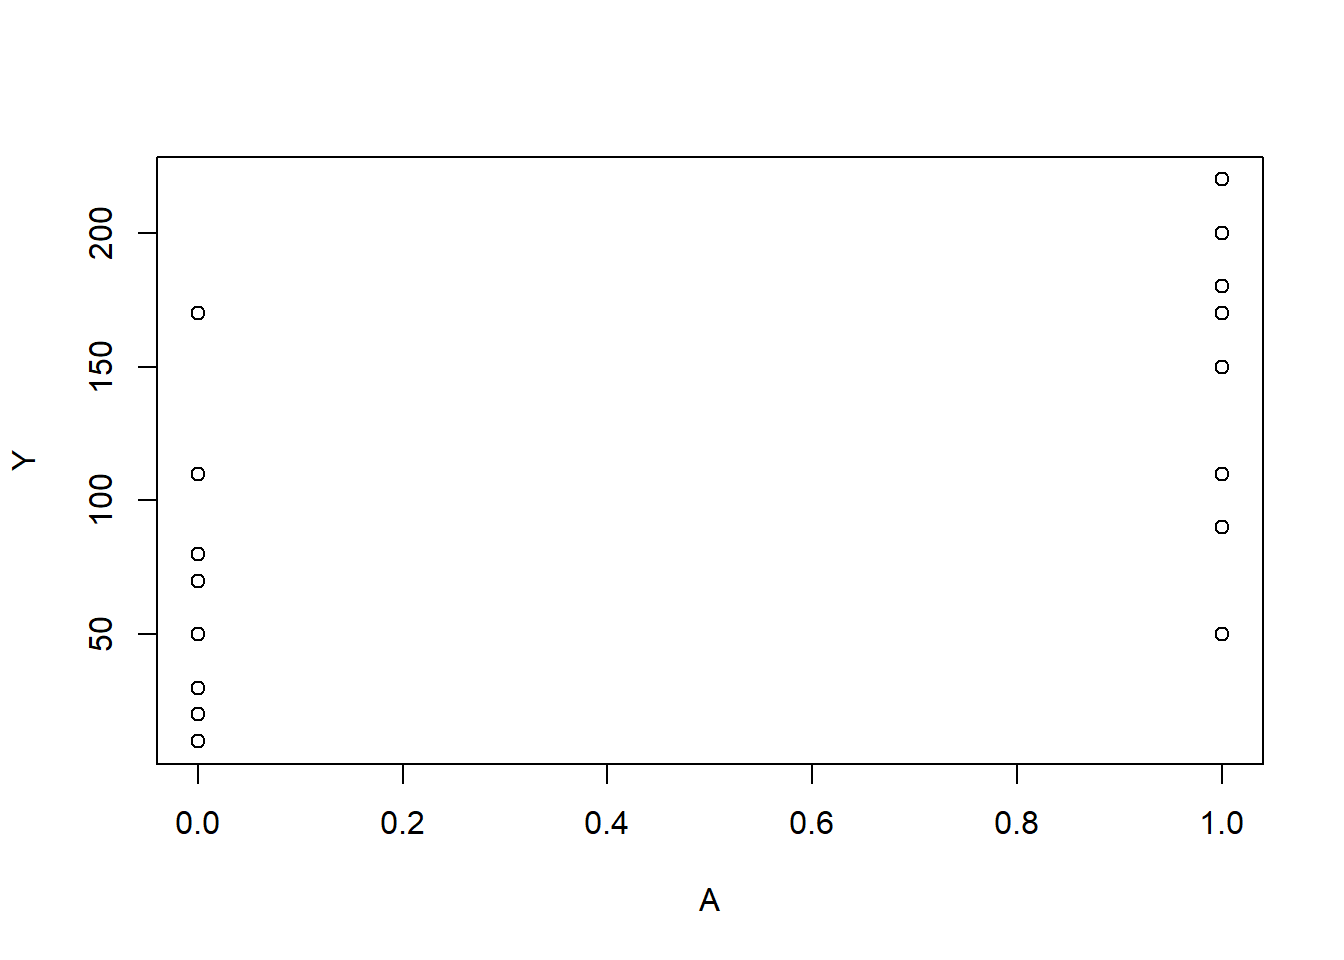
\includegraphics[width=0.85\linewidth]{11-why-model-r_files/figure-latex/unnamed-chunk-1-1} \end{center}

\begin{Shaded}
\begin{Highlighting}[]
\FunctionTok{summary}\NormalTok{(Y[A }\SpecialCharTok{==} \DecValTok{0}\NormalTok{])}
\end{Highlighting}
\end{Shaded}

\begin{verbatim}
##    Min. 1st Qu.  Median    Mean 3rd Qu.    Max. 
##    10.0    27.5    60.0    67.5    87.5   170.0
\end{verbatim}

\begin{Shaded}
\begin{Highlighting}[]
\FunctionTok{summary}\NormalTok{(Y[A }\SpecialCharTok{==} \DecValTok{1}\NormalTok{])}
\end{Highlighting}
\end{Shaded}

\begin{verbatim}
##    Min. 1st Qu.  Median    Mean 3rd Qu.    Max. 
##    50.0   105.0   160.0   146.2   185.0   220.0
\end{verbatim}

\begin{Shaded}
\begin{Highlighting}[]
\NormalTok{A2 }\OtherTok{\textless{}{-}} \FunctionTok{c}\NormalTok{(}\DecValTok{1}\NormalTok{, }\DecValTok{1}\NormalTok{, }\DecValTok{1}\NormalTok{, }\DecValTok{1}\NormalTok{, }\DecValTok{2}\NormalTok{, }\DecValTok{2}\NormalTok{, }\DecValTok{2}\NormalTok{, }\DecValTok{2}\NormalTok{, }\DecValTok{3}\NormalTok{, }\DecValTok{3}\NormalTok{, }\DecValTok{3}\NormalTok{, }\DecValTok{3}\NormalTok{, }\DecValTok{4}\NormalTok{, }\DecValTok{4}\NormalTok{, }\DecValTok{4}\NormalTok{, }\DecValTok{4}\NormalTok{)}
\NormalTok{Y2 }\OtherTok{\textless{}{-}} \FunctionTok{c}\NormalTok{(}\DecValTok{110}\NormalTok{, }\DecValTok{80}\NormalTok{, }\DecValTok{50}\NormalTok{, }\DecValTok{40}\NormalTok{, }\DecValTok{170}\NormalTok{, }\DecValTok{30}\NormalTok{, }\DecValTok{70}\NormalTok{, }\DecValTok{50}\NormalTok{, }\DecValTok{110}\NormalTok{, }\DecValTok{50}\NormalTok{, }\DecValTok{180}\NormalTok{,}
        \DecValTok{130}\NormalTok{, }\DecValTok{200}\NormalTok{, }\DecValTok{150}\NormalTok{, }\DecValTok{220}\NormalTok{, }\DecValTok{210}\NormalTok{)}

\FunctionTok{plot}\NormalTok{(A2, Y2)}
\end{Highlighting}
\end{Shaded}

\begin{center}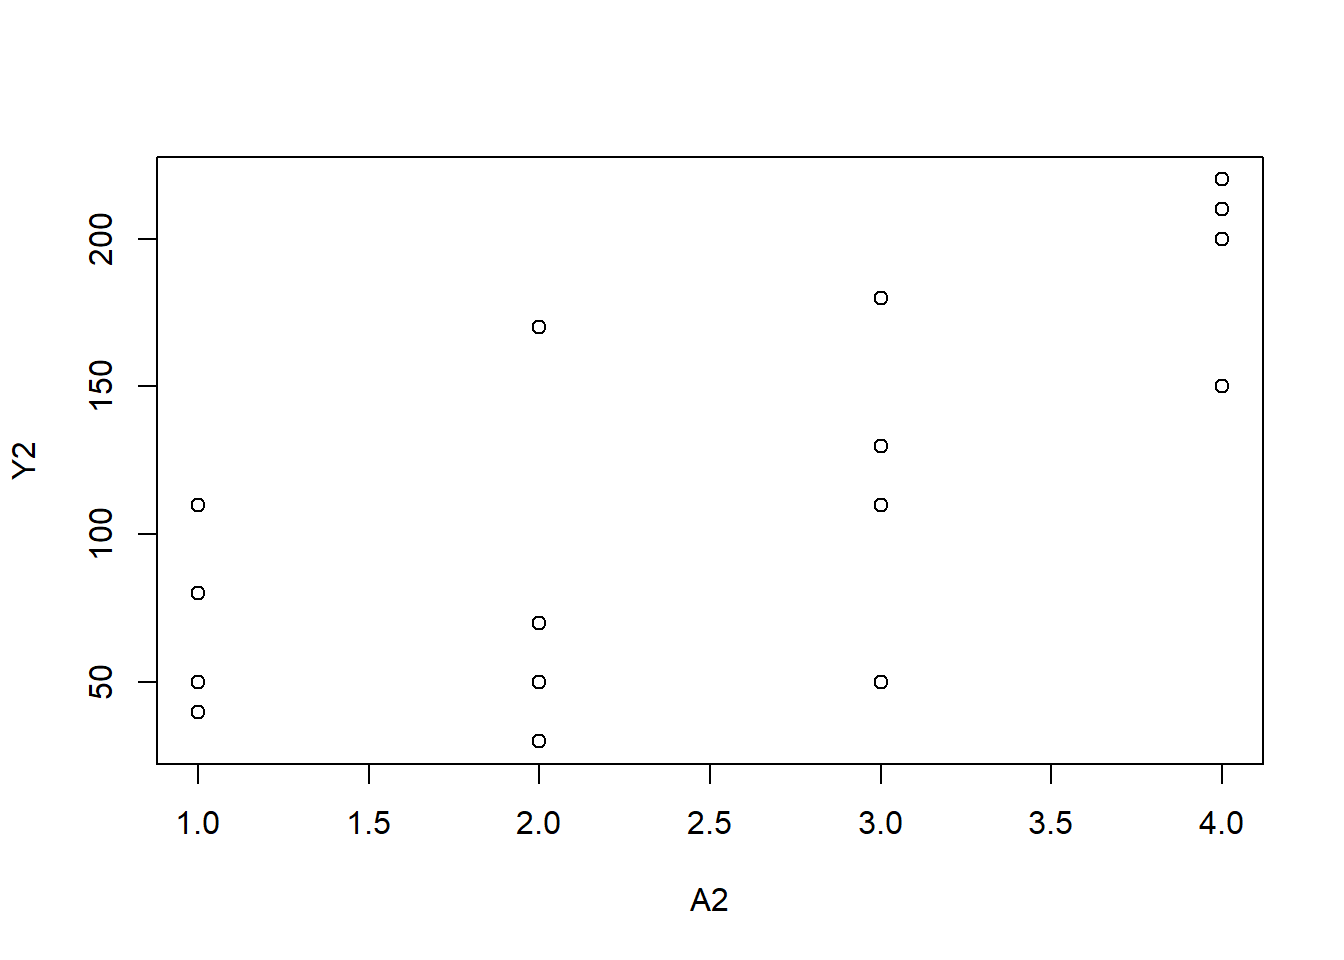
\includegraphics[width=0.85\linewidth]{11-why-model-r_files/figure-latex/unnamed-chunk-1-2} \end{center}

\begin{Shaded}
\begin{Highlighting}[]
\FunctionTok{summary}\NormalTok{(Y2[A2 }\SpecialCharTok{==} \DecValTok{1}\NormalTok{])}
\end{Highlighting}
\end{Shaded}

\begin{verbatim}
##    Min. 1st Qu.  Median    Mean 3rd Qu.    Max. 
##    40.0    47.5    65.0    70.0    87.5   110.0
\end{verbatim}

\begin{Shaded}
\begin{Highlighting}[]
\FunctionTok{summary}\NormalTok{(Y2[A2 }\SpecialCharTok{==} \DecValTok{2}\NormalTok{])}
\end{Highlighting}
\end{Shaded}

\begin{verbatim}
##    Min. 1st Qu.  Median    Mean 3rd Qu.    Max. 
##      30      45      60      80      95     170
\end{verbatim}

\begin{Shaded}
\begin{Highlighting}[]
\FunctionTok{summary}\NormalTok{(Y2[A2 }\SpecialCharTok{==} \DecValTok{3}\NormalTok{])}
\end{Highlighting}
\end{Shaded}

\begin{verbatim}
##    Min. 1st Qu.  Median    Mean 3rd Qu.    Max. 
##    50.0    95.0   120.0   117.5   142.5   180.0
\end{verbatim}

\begin{Shaded}
\begin{Highlighting}[]
\FunctionTok{summary}\NormalTok{(Y2[A2 }\SpecialCharTok{==} \DecValTok{4}\NormalTok{])}
\end{Highlighting}
\end{Shaded}

\begin{verbatim}
##    Min. 1st Qu.  Median    Mean 3rd Qu.    Max. 
##   150.0   187.5   205.0   195.0   212.5   220.0
\end{verbatim}

\hypertarget{program-11.2}{%
\section{Program 11.2}\label{program-11.2}}

\begin{itemize}
\tightlist
\item
  2-parameter linear model
\item
  Data from Figures 11.3 and 11.1
\end{itemize}

\begin{Shaded}
\begin{Highlighting}[]
\NormalTok{A3 }\OtherTok{\textless{}{-}}
  \FunctionTok{c}\NormalTok{(}\DecValTok{3}\NormalTok{, }\DecValTok{11}\NormalTok{, }\DecValTok{17}\NormalTok{, }\DecValTok{23}\NormalTok{, }\DecValTok{29}\NormalTok{, }\DecValTok{37}\NormalTok{, }\DecValTok{41}\NormalTok{, }\DecValTok{53}\NormalTok{, }\DecValTok{67}\NormalTok{, }\DecValTok{79}\NormalTok{, }\DecValTok{83}\NormalTok{, }\DecValTok{97}\NormalTok{, }\DecValTok{60}\NormalTok{, }\DecValTok{71}\NormalTok{, }\DecValTok{15}\NormalTok{, }\DecValTok{45}\NormalTok{)}
\NormalTok{Y3 }\OtherTok{\textless{}{-}}
  \FunctionTok{c}\NormalTok{(}\DecValTok{21}\NormalTok{, }\DecValTok{54}\NormalTok{, }\DecValTok{33}\NormalTok{, }\DecValTok{101}\NormalTok{, }\DecValTok{85}\NormalTok{, }\DecValTok{65}\NormalTok{, }\DecValTok{157}\NormalTok{, }\DecValTok{120}\NormalTok{, }\DecValTok{111}\NormalTok{, }\DecValTok{200}\NormalTok{, }\DecValTok{140}\NormalTok{, }\DecValTok{220}\NormalTok{, }\DecValTok{230}\NormalTok{, }\DecValTok{217}\NormalTok{,}
    \DecValTok{11}\NormalTok{, }\DecValTok{190}\NormalTok{)}

\FunctionTok{plot}\NormalTok{(Y3 }\SpecialCharTok{\textasciitilde{}}\NormalTok{ A3)}
\end{Highlighting}
\end{Shaded}

\begin{center}\includegraphics[width=0.85\linewidth]{11-why-model-r_files/figure-latex/unnamed-chunk-2-1} \end{center}

\begin{Shaded}
\begin{Highlighting}[]
\FunctionTok{summary}\NormalTok{(}\FunctionTok{glm}\NormalTok{(Y3 }\SpecialCharTok{\textasciitilde{}}\NormalTok{ A3))}
\end{Highlighting}
\end{Shaded}

\begin{verbatim}
## 
## Call:
## glm(formula = Y3 ~ A3)
## 
## Deviance Residuals: 
##     Min       1Q   Median       3Q      Max  
## -61.930  -30.564   -5.741   30.653   77.225  
## 
## Coefficients:
##             Estimate Std. Error t value Pr(>|t|)    
## (Intercept)  24.5464    21.3300   1.151 0.269094    
## A3            2.1372     0.3997   5.347 0.000103 ***
## ---
## Signif. codes:  0 '***' 0.001 '**' 0.01 '*' 0.05 '.' 0.1 ' ' 1
## 
## (Dispersion parameter for gaussian family taken to be 1944.109)
## 
##     Null deviance: 82800  on 15  degrees of freedom
## Residual deviance: 27218  on 14  degrees of freedom
## AIC: 170.43
## 
## Number of Fisher Scoring iterations: 2
\end{verbatim}

\begin{Shaded}
\begin{Highlighting}[]
\FunctionTok{predict}\NormalTok{(}\FunctionTok{glm}\NormalTok{(Y3 }\SpecialCharTok{\textasciitilde{}}\NormalTok{ A3), }\FunctionTok{data.frame}\NormalTok{(}\AttributeTok{A3 =} \DecValTok{90}\NormalTok{))}
\end{Highlighting}
\end{Shaded}

\begin{verbatim}
##      1 
## 216.89
\end{verbatim}

\begin{Shaded}
\begin{Highlighting}[]
\FunctionTok{summary}\NormalTok{(}\FunctionTok{glm}\NormalTok{(Y }\SpecialCharTok{\textasciitilde{}}\NormalTok{ A))}
\end{Highlighting}
\end{Shaded}

\begin{verbatim}
## 
## Call:
## glm(formula = Y ~ A)
## 
## Deviance Residuals: 
##     Min       1Q   Median       3Q      Max  
## -96.250  -40.000    3.125   35.938  102.500  
## 
## Coefficients:
##             Estimate Std. Error t value Pr(>|t|)   
## (Intercept)    67.50      19.72   3.424  0.00412 **
## A              78.75      27.88   2.824  0.01352 * 
## ---
## Signif. codes:  0 '***' 0.001 '**' 0.01 '*' 0.05 '.' 0.1 ' ' 1
## 
## (Dispersion parameter for gaussian family taken to be 3109.821)
## 
##     Null deviance: 68344  on 15  degrees of freedom
## Residual deviance: 43538  on 14  degrees of freedom
## AIC: 177.95
## 
## Number of Fisher Scoring iterations: 2
\end{verbatim}

\hypertarget{program-11.3}{%
\section{Program 11.3}\label{program-11.3}}

\begin{itemize}
\tightlist
\item
  3-parameter linear model
\item
  Data from Figure 11.3
\end{itemize}

\begin{Shaded}
\begin{Highlighting}[]
\NormalTok{Asq }\OtherTok{\textless{}{-}}\NormalTok{ A3 }\SpecialCharTok{*}\NormalTok{ A3}

\NormalTok{mod3 }\OtherTok{\textless{}{-}} \FunctionTok{glm}\NormalTok{(Y3 }\SpecialCharTok{\textasciitilde{}}\NormalTok{ A3 }\SpecialCharTok{+}\NormalTok{ Asq)}
\FunctionTok{summary}\NormalTok{(mod3)}
\end{Highlighting}
\end{Shaded}

\begin{verbatim}
## 
## Call:
## glm(formula = Y3 ~ A3 + Asq)
## 
## Deviance Residuals: 
##    Min      1Q  Median      3Q     Max  
## -65.27  -34.41   13.21   26.11   64.36  
## 
## Coefficients:
##             Estimate Std. Error t value Pr(>|t|)  
## (Intercept) -7.40688   31.74777  -0.233   0.8192  
## A3           4.10723    1.53088   2.683   0.0188 *
## Asq         -0.02038    0.01532  -1.331   0.2062  
## ---
## Signif. codes:  0 '***' 0.001 '**' 0.01 '*' 0.05 '.' 0.1 ' ' 1
## 
## (Dispersion parameter for gaussian family taken to be 1842.697)
## 
##     Null deviance: 82800  on 15  degrees of freedom
## Residual deviance: 23955  on 13  degrees of freedom
## AIC: 170.39
## 
## Number of Fisher Scoring iterations: 2
\end{verbatim}

\begin{Shaded}
\begin{Highlighting}[]
\FunctionTok{predict}\NormalTok{(mod3, }\FunctionTok{data.frame}\NormalTok{(}\FunctionTok{cbind}\NormalTok{(}\AttributeTok{A3 =} \DecValTok{90}\NormalTok{, }\AttributeTok{Asq =} \DecValTok{8100}\NormalTok{)))}
\end{Highlighting}
\end{Shaded}

\begin{verbatim}
##        1 
## 197.1269
\end{verbatim}

\hypertarget{ip-weighting-and-marginal-structural-models}{%
\chapter*{12. IP Weighting and Marginal Structural Models}\label{ip-weighting-and-marginal-structural-models}}
\addcontentsline{toc}{chapter}{12. IP Weighting and Marginal Structural Models}

\hypertarget{program-12.1}{%
\section{Program 12.1}\label{program-12.1}}

\begin{itemize}
\tightlist
\item
  Descriptive statistics from NHEFS data (Table 12.1)
\end{itemize}

\begin{Shaded}
\begin{Highlighting}[]
\FunctionTok{library}\NormalTok{(here)}
\end{Highlighting}
\end{Shaded}

\begin{Shaded}
\begin{Highlighting}[]
\CommentTok{\# install.packages("readxl") \# install package if required}
\FunctionTok{library}\NormalTok{(}\StringTok{"readxl"}\NormalTok{)}

\NormalTok{nhefs }\OtherTok{\textless{}{-}} \FunctionTok{read\_excel}\NormalTok{(}\FunctionTok{here}\NormalTok{(}\StringTok{"data"}\NormalTok{, }\StringTok{"NHEFS.xls"}\NormalTok{))}
\NormalTok{nhefs}\SpecialCharTok{$}\NormalTok{cens }\OtherTok{\textless{}{-}} \FunctionTok{ifelse}\NormalTok{(}\FunctionTok{is.na}\NormalTok{(nhefs}\SpecialCharTok{$}\NormalTok{wt82), }\DecValTok{1}\NormalTok{, }\DecValTok{0}\NormalTok{)}

\CommentTok{\# provisionally ignore subjects with missing values for weight in 1982}
\NormalTok{nhefs.nmv }\OtherTok{\textless{}{-}}
\NormalTok{  nhefs[}\FunctionTok{which}\NormalTok{(}\SpecialCharTok{!}\FunctionTok{is.na}\NormalTok{(nhefs}\SpecialCharTok{$}\NormalTok{wt82)),] }

\FunctionTok{lm}\NormalTok{(wt82\_71 }\SpecialCharTok{\textasciitilde{}}\NormalTok{ qsmk, }\AttributeTok{data =}\NormalTok{ nhefs.nmv)}
\end{Highlighting}
\end{Shaded}

\begin{verbatim}
## 
## Call:
## lm(formula = wt82_71 ~ qsmk, data = nhefs.nmv)
## 
## Coefficients:
## (Intercept)         qsmk  
##       1.984        2.541
\end{verbatim}

\begin{Shaded}
\begin{Highlighting}[]
\CommentTok{\# Smoking cessation}
\FunctionTok{predict}\NormalTok{(}\FunctionTok{lm}\NormalTok{(wt82\_71 }\SpecialCharTok{\textasciitilde{}}\NormalTok{ qsmk, }\AttributeTok{data =}\NormalTok{ nhefs.nmv), }\FunctionTok{data.frame}\NormalTok{(}\AttributeTok{qsmk =} \DecValTok{1}\NormalTok{))}
\end{Highlighting}
\end{Shaded}

\begin{verbatim}
##        1 
## 4.525079
\end{verbatim}

\begin{Shaded}
\begin{Highlighting}[]
\CommentTok{\# No smoking cessation}
\FunctionTok{predict}\NormalTok{(}\FunctionTok{lm}\NormalTok{(wt82\_71 }\SpecialCharTok{\textasciitilde{}}\NormalTok{ qsmk, }\AttributeTok{data =}\NormalTok{ nhefs.nmv), }\FunctionTok{data.frame}\NormalTok{(}\AttributeTok{qsmk =} \DecValTok{0}\NormalTok{)) }
\end{Highlighting}
\end{Shaded}

\begin{verbatim}
##        1 
## 1.984498
\end{verbatim}

\begin{Shaded}
\begin{Highlighting}[]
\CommentTok{\# Table}
\FunctionTok{summary}\NormalTok{(nhefs.nmv[}\FunctionTok{which}\NormalTok{(nhefs.nmv}\SpecialCharTok{$}\NormalTok{qsmk }\SpecialCharTok{==} \DecValTok{0}\NormalTok{),]}\SpecialCharTok{$}\NormalTok{age)}
\end{Highlighting}
\end{Shaded}

\begin{verbatim}
##    Min. 1st Qu.  Median    Mean 3rd Qu.    Max. 
##   25.00   33.00   42.00   42.79   51.00   72.00
\end{verbatim}

\begin{Shaded}
\begin{Highlighting}[]
\FunctionTok{summary}\NormalTok{(nhefs.nmv[}\FunctionTok{which}\NormalTok{(nhefs.nmv}\SpecialCharTok{$}\NormalTok{qsmk }\SpecialCharTok{==} \DecValTok{0}\NormalTok{),]}\SpecialCharTok{$}\NormalTok{wt71)}
\end{Highlighting}
\end{Shaded}

\begin{verbatim}
##    Min. 1st Qu.  Median    Mean 3rd Qu.    Max. 
##   40.82   59.19   68.49   70.30   79.38  151.73
\end{verbatim}

\begin{Shaded}
\begin{Highlighting}[]
\FunctionTok{summary}\NormalTok{(nhefs.nmv[}\FunctionTok{which}\NormalTok{(nhefs.nmv}\SpecialCharTok{$}\NormalTok{qsmk }\SpecialCharTok{==} \DecValTok{0}\NormalTok{),]}\SpecialCharTok{$}\NormalTok{smokeintensity)}
\end{Highlighting}
\end{Shaded}

\begin{verbatim}
##    Min. 1st Qu.  Median    Mean 3rd Qu.    Max. 
##    1.00   15.00   20.00   21.19   30.00   60.00
\end{verbatim}

\begin{Shaded}
\begin{Highlighting}[]
\FunctionTok{summary}\NormalTok{(nhefs.nmv[}\FunctionTok{which}\NormalTok{(nhefs.nmv}\SpecialCharTok{$}\NormalTok{qsmk }\SpecialCharTok{==} \DecValTok{0}\NormalTok{),]}\SpecialCharTok{$}\NormalTok{smokeyrs)}
\end{Highlighting}
\end{Shaded}

\begin{verbatim}
##    Min. 1st Qu.  Median    Mean 3rd Qu.    Max. 
##    1.00   15.00   23.00   24.09   32.00   64.00
\end{verbatim}

\begin{Shaded}
\begin{Highlighting}[]
\FunctionTok{summary}\NormalTok{(nhefs.nmv[}\FunctionTok{which}\NormalTok{(nhefs.nmv}\SpecialCharTok{$}\NormalTok{qsmk }\SpecialCharTok{==} \DecValTok{1}\NormalTok{),]}\SpecialCharTok{$}\NormalTok{age)}
\end{Highlighting}
\end{Shaded}

\begin{verbatim}
##    Min. 1st Qu.  Median    Mean 3rd Qu.    Max. 
##   25.00   35.00   46.00   46.17   56.00   74.00
\end{verbatim}

\begin{Shaded}
\begin{Highlighting}[]
\FunctionTok{summary}\NormalTok{(nhefs.nmv[}\FunctionTok{which}\NormalTok{(nhefs.nmv}\SpecialCharTok{$}\NormalTok{qsmk }\SpecialCharTok{==} \DecValTok{1}\NormalTok{),]}\SpecialCharTok{$}\NormalTok{wt71)}
\end{Highlighting}
\end{Shaded}

\begin{verbatim}
##    Min. 1st Qu.  Median    Mean 3rd Qu.    Max. 
##   39.58   60.67   71.21   72.35   81.08  136.98
\end{verbatim}

\begin{Shaded}
\begin{Highlighting}[]
\FunctionTok{summary}\NormalTok{(nhefs.nmv[}\FunctionTok{which}\NormalTok{(nhefs.nmv}\SpecialCharTok{$}\NormalTok{qsmk }\SpecialCharTok{==} \DecValTok{1}\NormalTok{),]}\SpecialCharTok{$}\NormalTok{smokeintensity)}
\end{Highlighting}
\end{Shaded}

\begin{verbatim}
##    Min. 1st Qu.  Median    Mean 3rd Qu.    Max. 
##     1.0    10.0    20.0    18.6    25.0    80.0
\end{verbatim}

\begin{Shaded}
\begin{Highlighting}[]
\FunctionTok{summary}\NormalTok{(nhefs.nmv[}\FunctionTok{which}\NormalTok{(nhefs.nmv}\SpecialCharTok{$}\NormalTok{qsmk }\SpecialCharTok{==} \DecValTok{1}\NormalTok{),]}\SpecialCharTok{$}\NormalTok{smokeyrs)}
\end{Highlighting}
\end{Shaded}

\begin{verbatim}
##    Min. 1st Qu.  Median    Mean 3rd Qu.    Max. 
##    1.00   15.00   26.00   26.03   35.00   60.00
\end{verbatim}

\begin{Shaded}
\begin{Highlighting}[]
\FunctionTok{table}\NormalTok{(nhefs.nmv}\SpecialCharTok{$}\NormalTok{qsmk, nhefs.nmv}\SpecialCharTok{$}\NormalTok{sex)}
\end{Highlighting}
\end{Shaded}

\begin{verbatim}
##    
##       0   1
##   0 542 621
##   1 220 183
\end{verbatim}

\begin{Shaded}
\begin{Highlighting}[]
\FunctionTok{prop.table}\NormalTok{(}\FunctionTok{table}\NormalTok{(nhefs.nmv}\SpecialCharTok{$}\NormalTok{qsmk, nhefs.nmv}\SpecialCharTok{$}\NormalTok{sex), }\DecValTok{1}\NormalTok{)}
\end{Highlighting}
\end{Shaded}

\begin{verbatim}
##    
##             0         1
##   0 0.4660361 0.5339639
##   1 0.5459057 0.4540943
\end{verbatim}

\begin{Shaded}
\begin{Highlighting}[]
\FunctionTok{table}\NormalTok{(nhefs.nmv}\SpecialCharTok{$}\NormalTok{qsmk, nhefs.nmv}\SpecialCharTok{$}\NormalTok{race)}
\end{Highlighting}
\end{Shaded}

\begin{verbatim}
##    
##       0   1
##   0 993 170
##   1 367  36
\end{verbatim}

\begin{Shaded}
\begin{Highlighting}[]
\FunctionTok{prop.table}\NormalTok{(}\FunctionTok{table}\NormalTok{(nhefs.nmv}\SpecialCharTok{$}\NormalTok{qsmk, nhefs.nmv}\SpecialCharTok{$}\NormalTok{race), }\DecValTok{1}\NormalTok{)}
\end{Highlighting}
\end{Shaded}

\begin{verbatim}
##    
##              0          1
##   0 0.85382631 0.14617369
##   1 0.91066998 0.08933002
\end{verbatim}

\begin{Shaded}
\begin{Highlighting}[]
\FunctionTok{table}\NormalTok{(nhefs.nmv}\SpecialCharTok{$}\NormalTok{qsmk, nhefs.nmv}\SpecialCharTok{$}\NormalTok{education)}
\end{Highlighting}
\end{Shaded}

\begin{verbatim}
##    
##       1   2   3   4   5
##   0 210 266 480  92 115
##   1  81  74 157  29  62
\end{verbatim}

\begin{Shaded}
\begin{Highlighting}[]
\FunctionTok{prop.table}\NormalTok{(}\FunctionTok{table}\NormalTok{(nhefs.nmv}\SpecialCharTok{$}\NormalTok{qsmk, nhefs.nmv}\SpecialCharTok{$}\NormalTok{education), }\DecValTok{1}\NormalTok{)}
\end{Highlighting}
\end{Shaded}

\begin{verbatim}
##    
##              1          2          3          4          5
##   0 0.18056750 0.22871883 0.41272571 0.07910576 0.09888220
##   1 0.20099256 0.18362283 0.38957816 0.07196030 0.15384615
\end{verbatim}

\begin{Shaded}
\begin{Highlighting}[]
\FunctionTok{table}\NormalTok{(nhefs.nmv}\SpecialCharTok{$}\NormalTok{qsmk, nhefs.nmv}\SpecialCharTok{$}\NormalTok{exercise)}
\end{Highlighting}
\end{Shaded}

\begin{verbatim}
##    
##       0   1   2
##   0 237 485 441
##   1  63 176 164
\end{verbatim}

\begin{Shaded}
\begin{Highlighting}[]
\FunctionTok{prop.table}\NormalTok{(}\FunctionTok{table}\NormalTok{(nhefs.nmv}\SpecialCharTok{$}\NormalTok{qsmk, nhefs.nmv}\SpecialCharTok{$}\NormalTok{exercise), }\DecValTok{1}\NormalTok{)}
\end{Highlighting}
\end{Shaded}

\begin{verbatim}
##    
##             0         1         2
##   0 0.2037833 0.4170249 0.3791917
##   1 0.1563275 0.4367246 0.4069479
\end{verbatim}

\begin{Shaded}
\begin{Highlighting}[]
\FunctionTok{table}\NormalTok{(nhefs.nmv}\SpecialCharTok{$}\NormalTok{qsmk, nhefs.nmv}\SpecialCharTok{$}\NormalTok{active)}
\end{Highlighting}
\end{Shaded}

\begin{verbatim}
##    
##       0   1   2
##   0 532 527 104
##   1 170 188  45
\end{verbatim}

\begin{Shaded}
\begin{Highlighting}[]
\FunctionTok{prop.table}\NormalTok{(}\FunctionTok{table}\NormalTok{(nhefs.nmv}\SpecialCharTok{$}\NormalTok{qsmk, nhefs.nmv}\SpecialCharTok{$}\NormalTok{active), }\DecValTok{1}\NormalTok{)}
\end{Highlighting}
\end{Shaded}

\begin{verbatim}
##    
##             0         1         2
##   0 0.4574377 0.4531384 0.0894239
##   1 0.4218362 0.4665012 0.1116625
\end{verbatim}

\hypertarget{program-12.2}{%
\section{Program 12.2}\label{program-12.2}}

\begin{itemize}
\tightlist
\item
  Estimating IP weights
\item
  Data from NHEFS
\end{itemize}

\begin{Shaded}
\begin{Highlighting}[]
\CommentTok{\# Estimation of ip weights via a logistic model}
\NormalTok{fit }\OtherTok{\textless{}{-}} \FunctionTok{glm}\NormalTok{(}
\NormalTok{  qsmk }\SpecialCharTok{\textasciitilde{}}\NormalTok{ sex }\SpecialCharTok{+}\NormalTok{ race }\SpecialCharTok{+}\NormalTok{ age }\SpecialCharTok{+} \FunctionTok{I}\NormalTok{(age }\SpecialCharTok{\^{}} \DecValTok{2}\NormalTok{) }\SpecialCharTok{+}
    \FunctionTok{as.factor}\NormalTok{(education) }\SpecialCharTok{+}\NormalTok{ smokeintensity }\SpecialCharTok{+}
    \FunctionTok{I}\NormalTok{(smokeintensity }\SpecialCharTok{\^{}} \DecValTok{2}\NormalTok{) }\SpecialCharTok{+}\NormalTok{ smokeyrs }\SpecialCharTok{+} \FunctionTok{I}\NormalTok{(smokeyrs }\SpecialCharTok{\^{}} \DecValTok{2}\NormalTok{) }\SpecialCharTok{+}
    \FunctionTok{as.factor}\NormalTok{(exercise) }\SpecialCharTok{+} \FunctionTok{as.factor}\NormalTok{(active) }\SpecialCharTok{+}\NormalTok{ wt71 }\SpecialCharTok{+} \FunctionTok{I}\NormalTok{(wt71 }\SpecialCharTok{\^{}} \DecValTok{2}\NormalTok{),}
  \AttributeTok{family =} \FunctionTok{binomial}\NormalTok{(),}
  \AttributeTok{data =}\NormalTok{ nhefs.nmv}
\NormalTok{)}
\FunctionTok{summary}\NormalTok{(fit)}
\end{Highlighting}
\end{Shaded}

\begin{verbatim}
## 
## Call:
## glm(formula = qsmk ~ sex + race + age + I(age^2) + as.factor(education) + 
##     smokeintensity + I(smokeintensity^2) + smokeyrs + I(smokeyrs^2) + 
##     as.factor(exercise) + as.factor(active) + wt71 + I(wt71^2), 
##     family = binomial(), data = nhefs.nmv)
## 
## Deviance Residuals: 
##     Min       1Q   Median       3Q      Max  
## -1.5127  -0.7907  -0.6387   0.9832   2.3729  
## 
## Coefficients:
##                         Estimate Std. Error z value Pr(>|z|)    
## (Intercept)           -2.2425191  1.3808360  -1.624 0.104369    
## sex                   -0.5274782  0.1540496  -3.424 0.000617 ***
## race                  -0.8392636  0.2100665  -3.995 6.46e-05 ***
## age                    0.1212052  0.0512663   2.364 0.018068 *  
## I(age^2)              -0.0008246  0.0005361  -1.538 0.124039    
## as.factor(education)2 -0.0287755  0.1983506  -0.145 0.884653    
## as.factor(education)3  0.0864318  0.1780850   0.485 0.627435    
## as.factor(education)4  0.0636010  0.2732108   0.233 0.815924    
## as.factor(education)5  0.4759606  0.2262237   2.104 0.035384 *  
## smokeintensity        -0.0772704  0.0152499  -5.067 4.04e-07 ***
## I(smokeintensity^2)    0.0010451  0.0002866   3.647 0.000265 ***
## smokeyrs              -0.0735966  0.0277775  -2.650 0.008061 ** 
## I(smokeyrs^2)          0.0008441  0.0004632   1.822 0.068398 .  
## as.factor(exercise)1   0.3548405  0.1801351   1.970 0.048855 *  
## as.factor(exercise)2   0.3957040  0.1872400   2.113 0.034571 *  
## as.factor(active)1     0.0319445  0.1329372   0.240 0.810100    
## as.factor(active)2     0.1767840  0.2149720   0.822 0.410873    
## wt71                  -0.0152357  0.0263161  -0.579 0.562625    
## I(wt71^2)              0.0001352  0.0001632   0.829 0.407370    
## ---
## Signif. codes:  0 '***' 0.001 '**' 0.01 '*' 0.05 '.' 0.1 ' ' 1
## 
## (Dispersion parameter for binomial family taken to be 1)
## 
##     Null deviance: 1786.1  on 1565  degrees of freedom
## Residual deviance: 1676.9  on 1547  degrees of freedom
## AIC: 1714.9
## 
## Number of Fisher Scoring iterations: 4
\end{verbatim}

\begin{Shaded}
\begin{Highlighting}[]
\NormalTok{p.qsmk.obs }\OtherTok{\textless{}{-}}
  \FunctionTok{ifelse}\NormalTok{(nhefs.nmv}\SpecialCharTok{$}\NormalTok{qsmk }\SpecialCharTok{==} \DecValTok{0}\NormalTok{,}
         \DecValTok{1} \SpecialCharTok{{-}} \FunctionTok{predict}\NormalTok{(fit, }\AttributeTok{type =} \StringTok{"response"}\NormalTok{),}
         \FunctionTok{predict}\NormalTok{(fit, }\AttributeTok{type =} \StringTok{"response"}\NormalTok{))}

\NormalTok{nhefs.nmv}\SpecialCharTok{$}\NormalTok{w }\OtherTok{\textless{}{-}} \DecValTok{1} \SpecialCharTok{/}\NormalTok{ p.qsmk.obs}
\FunctionTok{summary}\NormalTok{(nhefs.nmv}\SpecialCharTok{$}\NormalTok{w)}
\end{Highlighting}
\end{Shaded}

\begin{verbatim}
##    Min. 1st Qu.  Median    Mean 3rd Qu.    Max. 
##   1.054   1.230   1.373   1.996   1.990  16.700
\end{verbatim}

\begin{Shaded}
\begin{Highlighting}[]
\FunctionTok{sd}\NormalTok{(nhefs.nmv}\SpecialCharTok{$}\NormalTok{w)}
\end{Highlighting}
\end{Shaded}

\begin{verbatim}
## [1] 1.474787
\end{verbatim}

\begin{Shaded}
\begin{Highlighting}[]
\CommentTok{\# install.packages("geepack") \# install package if required}
\FunctionTok{library}\NormalTok{(}\StringTok{"geepack"}\NormalTok{)}
\NormalTok{msm.w }\OtherTok{\textless{}{-}} \FunctionTok{geeglm}\NormalTok{(}
\NormalTok{  wt82\_71 }\SpecialCharTok{\textasciitilde{}}\NormalTok{ qsmk,}
  \AttributeTok{data =}\NormalTok{ nhefs.nmv,}
  \AttributeTok{weights =}\NormalTok{ w,}
  \AttributeTok{id =}\NormalTok{ seqn,}
  \AttributeTok{corstr =} \StringTok{"independence"}
\NormalTok{)}
\FunctionTok{summary}\NormalTok{(msm.w)}
\end{Highlighting}
\end{Shaded}

\begin{verbatim}
## 
## Call:
## geeglm(formula = wt82_71 ~ qsmk, data = nhefs.nmv, weights = w, 
##     id = seqn, corstr = "independence")
## 
##  Coefficients:
##             Estimate Std.err  Wald Pr(>|W|)    
## (Intercept)   1.7800  0.2247 62.73 2.33e-15 ***
## qsmk          3.4405  0.5255 42.87 5.86e-11 ***
## ---
## Signif. codes:  0 '***' 0.001 '**' 0.01 '*' 0.05 '.' 0.1 ' ' 1
## 
## Correlation structure = independence 
## Estimated Scale Parameters:
## 
##             Estimate Std.err
## (Intercept)    65.06   4.221
## Number of clusters:   1566  Maximum cluster size: 1
\end{verbatim}

\begin{Shaded}
\begin{Highlighting}[]
\NormalTok{beta }\OtherTok{\textless{}{-}} \FunctionTok{coef}\NormalTok{(msm.w)}
\NormalTok{SE }\OtherTok{\textless{}{-}} \FunctionTok{coef}\NormalTok{(}\FunctionTok{summary}\NormalTok{(msm.w))[, }\DecValTok{2}\NormalTok{]}
\NormalTok{lcl }\OtherTok{\textless{}{-}}\NormalTok{ beta }\SpecialCharTok{{-}} \FunctionTok{qnorm}\NormalTok{(}\FloatTok{0.975}\NormalTok{) }\SpecialCharTok{*}\NormalTok{ SE}
\NormalTok{ucl }\OtherTok{\textless{}{-}}\NormalTok{ beta }\SpecialCharTok{+} \FunctionTok{qnorm}\NormalTok{(}\FloatTok{0.975}\NormalTok{) }\SpecialCharTok{*}\NormalTok{ SE}
\FunctionTok{cbind}\NormalTok{(beta, lcl, ucl)}
\end{Highlighting}
\end{Shaded}

\begin{verbatim}
##              beta   lcl  ucl
## (Intercept) 1.780 1.340 2.22
## qsmk        3.441 2.411 4.47
\end{verbatim}

\begin{Shaded}
\begin{Highlighting}[]
\CommentTok{\# no association between sex and qsmk in pseudo{-}population}
\FunctionTok{xtabs}\NormalTok{(nhefs.nmv}\SpecialCharTok{$}\NormalTok{w }\SpecialCharTok{\textasciitilde{}}\NormalTok{ nhefs.nmv}\SpecialCharTok{$}\NormalTok{sex }\SpecialCharTok{+}\NormalTok{ nhefs.nmv}\SpecialCharTok{$}\NormalTok{qsmk)}
\end{Highlighting}
\end{Shaded}

\begin{verbatim}
##              nhefs.nmv$qsmk
## nhefs.nmv$sex     0     1
##             0 763.6 763.6
##             1 801.7 797.2
\end{verbatim}

\begin{Shaded}
\begin{Highlighting}[]
\CommentTok{\# "check" for positivity (White women)}
\FunctionTok{table}\NormalTok{(nhefs.nmv}\SpecialCharTok{$}\NormalTok{age[nhefs.nmv}\SpecialCharTok{$}\NormalTok{race }\SpecialCharTok{==} \DecValTok{0} \SpecialCharTok{\&}\NormalTok{ nhefs.nmv}\SpecialCharTok{$}\NormalTok{sex }\SpecialCharTok{==} \DecValTok{1}\NormalTok{],}
\NormalTok{      nhefs.nmv}\SpecialCharTok{$}\NormalTok{qsmk[nhefs.nmv}\SpecialCharTok{$}\NormalTok{race }\SpecialCharTok{==} \DecValTok{0} \SpecialCharTok{\&}\NormalTok{ nhefs.nmv}\SpecialCharTok{$}\NormalTok{sex }\SpecialCharTok{==} \DecValTok{1}\NormalTok{])}
\end{Highlighting}
\end{Shaded}

\begin{verbatim}
##     
##       0  1
##   25 24  3
##   26 14  5
##   27 18  2
##   28 20  5
##   29 15  4
##   30 14  5
##   31 11  5
##   32 14  7
##   33 12  3
##   34 22  5
##   35 16  5
##   36 13  3
##   37 14  1
##   38  6  2
##   39 19  4
##   40 10  4
##   41 13  3
##   42 16  3
##   43 14  3
##   44  9  4
##   45 12  5
##   46 19  4
##   47 19  4
##   48 19  4
##   49 11  3
##   50 18  4
##   51  9  3
##   52 11  3
##   53 11  4
##   54 17  9
##   55  9  4
##   56  8  7
##   57  9  2
##   58  8  4
##   59  5  4
##   60  5  4
##   61  5  2
##   62  6  5
##   63  3  3
##   64  7  1
##   65  3  2
##   66  4  0
##   67  2  0
##   69  6  2
##   70  2  1
##   71  0  1
##   72  2  2
##   74  0  1
\end{verbatim}

\hypertarget{program-12.3}{%
\section{Program 12.3}\label{program-12.3}}

\begin{itemize}
\tightlist
\item
  Estimating stabilized IP weights
\item
  Data from NHEFS
\end{itemize}

\begin{Shaded}
\begin{Highlighting}[]
\CommentTok{\# estimation of denominator of ip weights}
\NormalTok{denom.fit }\OtherTok{\textless{}{-}}
  \FunctionTok{glm}\NormalTok{(}
\NormalTok{    qsmk }\SpecialCharTok{\textasciitilde{}} \FunctionTok{as.factor}\NormalTok{(sex) }\SpecialCharTok{+} \FunctionTok{as.factor}\NormalTok{(race) }\SpecialCharTok{+}\NormalTok{ age }\SpecialCharTok{+} \FunctionTok{I}\NormalTok{(age }\SpecialCharTok{\^{}} \DecValTok{2}\NormalTok{) }\SpecialCharTok{+}
      \FunctionTok{as.factor}\NormalTok{(education) }\SpecialCharTok{+}\NormalTok{ smokeintensity }\SpecialCharTok{+}
      \FunctionTok{I}\NormalTok{(smokeintensity }\SpecialCharTok{\^{}} \DecValTok{2}\NormalTok{) }\SpecialCharTok{+}\NormalTok{ smokeyrs }\SpecialCharTok{+} \FunctionTok{I}\NormalTok{(smokeyrs }\SpecialCharTok{\^{}} \DecValTok{2}\NormalTok{) }\SpecialCharTok{+}
      \FunctionTok{as.factor}\NormalTok{(exercise) }\SpecialCharTok{+} \FunctionTok{as.factor}\NormalTok{(active) }\SpecialCharTok{+}\NormalTok{ wt71 }\SpecialCharTok{+} \FunctionTok{I}\NormalTok{(wt71 }\SpecialCharTok{\^{}} \DecValTok{2}\NormalTok{),}
    \AttributeTok{family =} \FunctionTok{binomial}\NormalTok{(),}
    \AttributeTok{data =}\NormalTok{ nhefs.nmv}
\NormalTok{  )}
\FunctionTok{summary}\NormalTok{(denom.fit)}
\end{Highlighting}
\end{Shaded}

\begin{verbatim}
## 
## Call:
## glm(formula = qsmk ~ as.factor(sex) + as.factor(race) + age + 
##     I(age^2) + as.factor(education) + smokeintensity + I(smokeintensity^2) + 
##     smokeyrs + I(smokeyrs^2) + as.factor(exercise) + as.factor(active) + 
##     wt71 + I(wt71^2), family = binomial(), data = nhefs.nmv)
## 
## Deviance Residuals: 
##    Min      1Q  Median      3Q     Max  
## -1.513  -0.791  -0.639   0.983   2.373  
## 
## Coefficients:
##                        Estimate Std. Error z value Pr(>|z|)    
## (Intercept)           -2.242519   1.380836   -1.62  0.10437    
## as.factor(sex)1       -0.527478   0.154050   -3.42  0.00062 ***
## as.factor(race)1      -0.839264   0.210067   -4.00  6.5e-05 ***
## age                    0.121205   0.051266    2.36  0.01807 *  
## I(age^2)              -0.000825   0.000536   -1.54  0.12404    
## as.factor(education)2 -0.028776   0.198351   -0.15  0.88465    
## as.factor(education)3  0.086432   0.178085    0.49  0.62744    
## as.factor(education)4  0.063601   0.273211    0.23  0.81592    
## as.factor(education)5  0.475961   0.226224    2.10  0.03538 *  
## smokeintensity        -0.077270   0.015250   -5.07  4.0e-07 ***
## I(smokeintensity^2)    0.001045   0.000287    3.65  0.00027 ***
## smokeyrs              -0.073597   0.027777   -2.65  0.00806 ** 
## I(smokeyrs^2)          0.000844   0.000463    1.82  0.06840 .  
## as.factor(exercise)1   0.354841   0.180135    1.97  0.04885 *  
## as.factor(exercise)2   0.395704   0.187240    2.11  0.03457 *  
## as.factor(active)1     0.031944   0.132937    0.24  0.81010    
## as.factor(active)2     0.176784   0.214972    0.82  0.41087    
## wt71                  -0.015236   0.026316   -0.58  0.56262    
## I(wt71^2)              0.000135   0.000163    0.83  0.40737    
## ---
## Signif. codes:  0 '***' 0.001 '**' 0.01 '*' 0.05 '.' 0.1 ' ' 1
## 
## (Dispersion parameter for binomial family taken to be 1)
## 
##     Null deviance: 1786.1  on 1565  degrees of freedom
## Residual deviance: 1676.9  on 1547  degrees of freedom
## AIC: 1715
## 
## Number of Fisher Scoring iterations: 4
\end{verbatim}

\begin{Shaded}
\begin{Highlighting}[]
\NormalTok{pd.qsmk }\OtherTok{\textless{}{-}} \FunctionTok{predict}\NormalTok{(denom.fit, }\AttributeTok{type =} \StringTok{"response"}\NormalTok{)}

\CommentTok{\# estimation of numerator of ip weights}
\NormalTok{numer.fit }\OtherTok{\textless{}{-}} \FunctionTok{glm}\NormalTok{(qsmk }\SpecialCharTok{\textasciitilde{}} \DecValTok{1}\NormalTok{, }\AttributeTok{family =} \FunctionTok{binomial}\NormalTok{(), }\AttributeTok{data =}\NormalTok{ nhefs.nmv)}
\FunctionTok{summary}\NormalTok{(numer.fit)}
\end{Highlighting}
\end{Shaded}

\begin{verbatim}
## 
## Call:
## glm(formula = qsmk ~ 1, family = binomial(), data = nhefs.nmv)
## 
## Deviance Residuals: 
##    Min      1Q  Median      3Q     Max  
## -0.771  -0.771  -0.771   1.648   1.648  
## 
## Coefficients:
##             Estimate Std. Error z value Pr(>|z|)    
## (Intercept)  -1.0598     0.0578   -18.3   <2e-16 ***
## ---
## Signif. codes:  0 '***' 0.001 '**' 0.01 '*' 0.05 '.' 0.1 ' ' 1
## 
## (Dispersion parameter for binomial family taken to be 1)
## 
##     Null deviance: 1786.1  on 1565  degrees of freedom
## Residual deviance: 1786.1  on 1565  degrees of freedom
## AIC: 1788
## 
## Number of Fisher Scoring iterations: 4
\end{verbatim}

\begin{Shaded}
\begin{Highlighting}[]
\NormalTok{pn.qsmk }\OtherTok{\textless{}{-}} \FunctionTok{predict}\NormalTok{(numer.fit, }\AttributeTok{type =} \StringTok{"response"}\NormalTok{)}

\NormalTok{nhefs.nmv}\SpecialCharTok{$}\NormalTok{sw }\OtherTok{\textless{}{-}}
  \FunctionTok{ifelse}\NormalTok{(nhefs.nmv}\SpecialCharTok{$}\NormalTok{qsmk }\SpecialCharTok{==} \DecValTok{0}\NormalTok{, ((}\DecValTok{1} \SpecialCharTok{{-}}\NormalTok{ pn.qsmk) }\SpecialCharTok{/}\NormalTok{ (}\DecValTok{1} \SpecialCharTok{{-}}\NormalTok{ pd.qsmk)),}
\NormalTok{         (pn.qsmk }\SpecialCharTok{/}\NormalTok{ pd.qsmk))}

\FunctionTok{summary}\NormalTok{(nhefs.nmv}\SpecialCharTok{$}\NormalTok{sw)}
\end{Highlighting}
\end{Shaded}

\begin{verbatim}
##    Min. 1st Qu.  Median    Mean 3rd Qu.    Max. 
##   0.331   0.867   0.950   0.999   1.079   4.298
\end{verbatim}

\begin{Shaded}
\begin{Highlighting}[]
\NormalTok{msm.sw }\OtherTok{\textless{}{-}} \FunctionTok{geeglm}\NormalTok{(}
\NormalTok{  wt82\_71 }\SpecialCharTok{\textasciitilde{}}\NormalTok{ qsmk,}
  \AttributeTok{data =}\NormalTok{ nhefs.nmv,}
  \AttributeTok{weights =}\NormalTok{ sw,}
  \AttributeTok{id =}\NormalTok{ seqn,}
  \AttributeTok{corstr =} \StringTok{"independence"}
\NormalTok{)}
\FunctionTok{summary}\NormalTok{(msm.sw)}
\end{Highlighting}
\end{Shaded}

\begin{verbatim}
## 
## Call:
## geeglm(formula = wt82_71 ~ qsmk, data = nhefs.nmv, weights = sw, 
##     id = seqn, corstr = "independence")
## 
##  Coefficients:
##             Estimate Std.err Wald Pr(>|W|)    
## (Intercept)    1.780   0.225 62.7  2.3e-15 ***
## qsmk           3.441   0.525 42.9  5.9e-11 ***
## ---
## Signif. codes:  0 '***' 0.001 '**' 0.01 '*' 0.05 '.' 0.1 ' ' 1
## 
## Correlation structure = independence 
## Estimated Scale Parameters:
## 
##             Estimate Std.err
## (Intercept)     60.7    3.71
## Number of clusters:   1566  Maximum cluster size: 1
\end{verbatim}

\begin{Shaded}
\begin{Highlighting}[]
\NormalTok{beta }\OtherTok{\textless{}{-}} \FunctionTok{coef}\NormalTok{(msm.sw)}
\NormalTok{SE }\OtherTok{\textless{}{-}} \FunctionTok{coef}\NormalTok{(}\FunctionTok{summary}\NormalTok{(msm.sw))[, }\DecValTok{2}\NormalTok{]}
\NormalTok{lcl }\OtherTok{\textless{}{-}}\NormalTok{ beta }\SpecialCharTok{{-}} \FunctionTok{qnorm}\NormalTok{(}\FloatTok{0.975}\NormalTok{) }\SpecialCharTok{*}\NormalTok{ SE}
\NormalTok{ucl }\OtherTok{\textless{}{-}}\NormalTok{ beta }\SpecialCharTok{+} \FunctionTok{qnorm}\NormalTok{(}\FloatTok{0.975}\NormalTok{) }\SpecialCharTok{*}\NormalTok{ SE}
\FunctionTok{cbind}\NormalTok{(beta, lcl, ucl)}
\end{Highlighting}
\end{Shaded}

\begin{verbatim}
##             beta  lcl  ucl
## (Intercept) 1.78 1.34 2.22
## qsmk        3.44 2.41 4.47
\end{verbatim}

\begin{Shaded}
\begin{Highlighting}[]
\CommentTok{\# no association between sex and qsmk in pseudo{-}population}
\FunctionTok{xtabs}\NormalTok{(nhefs.nmv}\SpecialCharTok{$}\NormalTok{sw }\SpecialCharTok{\textasciitilde{}}\NormalTok{ nhefs.nmv}\SpecialCharTok{$}\NormalTok{sex }\SpecialCharTok{+}\NormalTok{ nhefs.nmv}\SpecialCharTok{$}\NormalTok{qsmk)}
\end{Highlighting}
\end{Shaded}

\begin{verbatim}
##              nhefs.nmv$qsmk
## nhefs.nmv$sex   0   1
##             0 567 197
##             1 595 205
\end{verbatim}

\hypertarget{program-12.4}{%
\section{Program 12.4}\label{program-12.4}}

\begin{itemize}
\tightlist
\item
  Estimating the parameters of a marginal structural mean model with a continuous treatment Data from NHEFS
\end{itemize}

\begin{Shaded}
\begin{Highlighting}[]
\CommentTok{\# Analysis restricted to subjects reporting \textless{}=25 cig/day at baseline}
\NormalTok{nhefs.nmv.s }\OtherTok{\textless{}{-}} \FunctionTok{subset}\NormalTok{(nhefs.nmv, smokeintensity }\SpecialCharTok{\textless{}=} \DecValTok{25}\NormalTok{)}

\CommentTok{\# estimation of denominator of ip weights}
\NormalTok{den.fit.obj }\OtherTok{\textless{}{-}} \FunctionTok{lm}\NormalTok{(}
\NormalTok{  smkintensity82\_71 }\SpecialCharTok{\textasciitilde{}} \FunctionTok{as.factor}\NormalTok{(sex) }\SpecialCharTok{+}
    \FunctionTok{as.factor}\NormalTok{(race) }\SpecialCharTok{+}\NormalTok{ age }\SpecialCharTok{+} \FunctionTok{I}\NormalTok{(age }\SpecialCharTok{\^{}} \DecValTok{2}\NormalTok{) }\SpecialCharTok{+}
    \FunctionTok{as.factor}\NormalTok{(education) }\SpecialCharTok{+}\NormalTok{ smokeintensity }\SpecialCharTok{+} \FunctionTok{I}\NormalTok{(smokeintensity }\SpecialCharTok{\^{}} \DecValTok{2}\NormalTok{) }\SpecialCharTok{+}
\NormalTok{    smokeyrs }\SpecialCharTok{+} \FunctionTok{I}\NormalTok{(smokeyrs }\SpecialCharTok{\^{}} \DecValTok{2}\NormalTok{) }\SpecialCharTok{+} \FunctionTok{as.factor}\NormalTok{(exercise) }\SpecialCharTok{+} \FunctionTok{as.factor}\NormalTok{(active) }\SpecialCharTok{+}\NormalTok{ wt71 }\SpecialCharTok{+}
    \FunctionTok{I}\NormalTok{(wt71 }\SpecialCharTok{\^{}} \DecValTok{2}\NormalTok{),}
  \AttributeTok{data =}\NormalTok{ nhefs.nmv.s}
\NormalTok{)}
\NormalTok{p.den }\OtherTok{\textless{}{-}} \FunctionTok{predict}\NormalTok{(den.fit.obj, }\AttributeTok{type =} \StringTok{"response"}\NormalTok{)}
\NormalTok{dens.den }\OtherTok{\textless{}{-}}
  \FunctionTok{dnorm}\NormalTok{(nhefs.nmv.s}\SpecialCharTok{$}\NormalTok{smkintensity82\_71,}
\NormalTok{        p.den,}
        \FunctionTok{summary}\NormalTok{(den.fit.obj)}\SpecialCharTok{$}\NormalTok{sigma)}

\CommentTok{\# estimation of numerator of ip weights}
\NormalTok{num.fit.obj }\OtherTok{\textless{}{-}} \FunctionTok{lm}\NormalTok{(smkintensity82\_71 }\SpecialCharTok{\textasciitilde{}} \DecValTok{1}\NormalTok{, }\AttributeTok{data =}\NormalTok{ nhefs.nmv.s)}
\NormalTok{p.num }\OtherTok{\textless{}{-}} \FunctionTok{predict}\NormalTok{(num.fit.obj, }\AttributeTok{type =} \StringTok{"response"}\NormalTok{)}
\NormalTok{dens.num }\OtherTok{\textless{}{-}}
  \FunctionTok{dnorm}\NormalTok{(nhefs.nmv.s}\SpecialCharTok{$}\NormalTok{smkintensity82\_71,}
\NormalTok{        p.num,}
        \FunctionTok{summary}\NormalTok{(num.fit.obj)}\SpecialCharTok{$}\NormalTok{sigma)}

\NormalTok{nhefs.nmv.s}\SpecialCharTok{$}\NormalTok{sw.a }\OtherTok{\textless{}{-}}\NormalTok{ dens.num }\SpecialCharTok{/}\NormalTok{ dens.den}
\FunctionTok{summary}\NormalTok{(nhefs.nmv.s}\SpecialCharTok{$}\NormalTok{sw.a)}
\end{Highlighting}
\end{Shaded}

\begin{verbatim}
##    Min. 1st Qu.  Median    Mean 3rd Qu.    Max. 
##    0.19    0.89    0.97    1.00    1.05    5.10
\end{verbatim}

\begin{Shaded}
\begin{Highlighting}[]
\NormalTok{msm.sw.cont }\OtherTok{\textless{}{-}}
  \FunctionTok{geeglm}\NormalTok{(}
\NormalTok{    wt82\_71 }\SpecialCharTok{\textasciitilde{}}\NormalTok{ smkintensity82\_71 }\SpecialCharTok{+} \FunctionTok{I}\NormalTok{(smkintensity82\_71 }\SpecialCharTok{*}\NormalTok{ smkintensity82\_71),}
    \AttributeTok{data =}\NormalTok{ nhefs.nmv.s,}
    \AttributeTok{weights =}\NormalTok{ sw.a,}
    \AttributeTok{id =}\NormalTok{ seqn,}
    \AttributeTok{corstr =} \StringTok{"independence"}
\NormalTok{  )}
\FunctionTok{summary}\NormalTok{(msm.sw.cont)}
\end{Highlighting}
\end{Shaded}

\begin{verbatim}
## 
## Call:
## geeglm(formula = wt82_71 ~ smkintensity82_71 + I(smkintensity82_71 * 
##     smkintensity82_71), data = nhefs.nmv.s, weights = sw.a, id = seqn, 
##     corstr = "independence")
## 
##  Coefficients:
##                                          Estimate  Std.err  Wald Pr(>|W|)    
## (Intercept)                               2.00452  0.29512 46.13  1.1e-11 ***
## smkintensity82_71                        -0.10899  0.03154 11.94  0.00055 ***
## I(smkintensity82_71 * smkintensity82_71)  0.00269  0.00242  1.24  0.26489    
## ---
## Signif. codes:  0 '***' 0.001 '**' 0.01 '*' 0.05 '.' 0.1 ' ' 1
## 
## Correlation structure = independence 
## Estimated Scale Parameters:
## 
##             Estimate Std.err
## (Intercept)     60.5     4.5
## Number of clusters:   1162  Maximum cluster size: 1
\end{verbatim}

\begin{Shaded}
\begin{Highlighting}[]
\NormalTok{beta }\OtherTok{\textless{}{-}} \FunctionTok{coef}\NormalTok{(msm.sw.cont)}
\NormalTok{SE }\OtherTok{\textless{}{-}} \FunctionTok{coef}\NormalTok{(}\FunctionTok{summary}\NormalTok{(msm.sw.cont))[, }\DecValTok{2}\NormalTok{]}
\NormalTok{lcl }\OtherTok{\textless{}{-}}\NormalTok{ beta }\SpecialCharTok{{-}} \FunctionTok{qnorm}\NormalTok{(}\FloatTok{0.975}\NormalTok{) }\SpecialCharTok{*}\NormalTok{ SE}
\NormalTok{ucl }\OtherTok{\textless{}{-}}\NormalTok{ beta }\SpecialCharTok{+} \FunctionTok{qnorm}\NormalTok{(}\FloatTok{0.975}\NormalTok{) }\SpecialCharTok{*}\NormalTok{ SE}
\FunctionTok{cbind}\NormalTok{(beta, lcl, ucl)}
\end{Highlighting}
\end{Shaded}

\begin{verbatim}
##                                              beta      lcl      ucl
## (Intercept)                               2.00452  1.42610  2.58295
## smkintensity82_71                        -0.10899 -0.17080 -0.04718
## I(smkintensity82_71 * smkintensity82_71)  0.00269 -0.00204  0.00743
\end{verbatim}

\hypertarget{program-12.5}{%
\section{Program 12.5}\label{program-12.5}}

\begin{itemize}
\tightlist
\item
  Estimating the parameters of a marginal structural logistic model
\item
  Data from NHEFS
\end{itemize}

\begin{Shaded}
\begin{Highlighting}[]
\FunctionTok{table}\NormalTok{(nhefs.nmv}\SpecialCharTok{$}\NormalTok{qsmk, nhefs.nmv}\SpecialCharTok{$}\NormalTok{death)}
\end{Highlighting}
\end{Shaded}

\begin{verbatim}
##    
##       0   1
##   0 963 200
##   1 312  91
\end{verbatim}

\begin{Shaded}
\begin{Highlighting}[]
\CommentTok{\# First, estimation of stabilized weights sw (same as in Program 12.3)}
\CommentTok{\# Second, fit logistic model below}
\NormalTok{msm.logistic }\OtherTok{\textless{}{-}} \FunctionTok{geeglm}\NormalTok{(}
\NormalTok{  death }\SpecialCharTok{\textasciitilde{}}\NormalTok{ qsmk,}
  \AttributeTok{data =}\NormalTok{ nhefs.nmv,}
  \AttributeTok{weights =}\NormalTok{ sw,}
  \AttributeTok{id =}\NormalTok{ seqn,}
  \AttributeTok{family =} \FunctionTok{binomial}\NormalTok{(),}
  \AttributeTok{corstr =} \StringTok{"independence"}
\NormalTok{)}
\end{Highlighting}
\end{Shaded}

\begin{verbatim}
## Warning in eval(family$initialize): non-integer #successes in a binomial glm!
\end{verbatim}

\begin{Shaded}
\begin{Highlighting}[]
\FunctionTok{summary}\NormalTok{(msm.logistic)}
\end{Highlighting}
\end{Shaded}

\begin{verbatim}
## 
## Call:
## geeglm(formula = death ~ qsmk, family = binomial(), data = nhefs.nmv, 
##     weights = sw, id = seqn, corstr = "independence")
## 
##  Coefficients:
##             Estimate Std.err   Wald Pr(>|W|)    
## (Intercept)  -1.4905  0.0789 356.50   <2e-16 ***
## qsmk          0.0301  0.1573   0.04     0.85    
## ---
## Signif. codes:  0 '***' 0.001 '**' 0.01 '*' 0.05 '.' 0.1 ' ' 1
## 
## Correlation structure = independence 
## Estimated Scale Parameters:
## 
##             Estimate Std.err
## (Intercept)        1  0.0678
## Number of clusters:   1566  Maximum cluster size: 1
\end{verbatim}

\begin{Shaded}
\begin{Highlighting}[]
\NormalTok{beta }\OtherTok{\textless{}{-}} \FunctionTok{coef}\NormalTok{(msm.logistic)}
\NormalTok{SE }\OtherTok{\textless{}{-}} \FunctionTok{coef}\NormalTok{(}\FunctionTok{summary}\NormalTok{(msm.logistic))[, }\DecValTok{2}\NormalTok{]}
\NormalTok{lcl }\OtherTok{\textless{}{-}}\NormalTok{ beta }\SpecialCharTok{{-}} \FunctionTok{qnorm}\NormalTok{(}\FloatTok{0.975}\NormalTok{) }\SpecialCharTok{*}\NormalTok{ SE}
\NormalTok{ucl }\OtherTok{\textless{}{-}}\NormalTok{ beta }\SpecialCharTok{+} \FunctionTok{qnorm}\NormalTok{(}\FloatTok{0.975}\NormalTok{) }\SpecialCharTok{*}\NormalTok{ SE}
\FunctionTok{cbind}\NormalTok{(beta, lcl, ucl)}
\end{Highlighting}
\end{Shaded}

\begin{verbatim}
##                beta    lcl    ucl
## (Intercept) -1.4905 -1.645 -1.336
## qsmk         0.0301 -0.278  0.338
\end{verbatim}

\hypertarget{program-12.6}{%
\section{Program 12.6}\label{program-12.6}}

\begin{itemize}
\tightlist
\item
  Assessing effect modification by sex using a marginal structural mean model
\item
  Data from NHEFS
\end{itemize}

\begin{Shaded}
\begin{Highlighting}[]
\FunctionTok{table}\NormalTok{(nhefs.nmv}\SpecialCharTok{$}\NormalTok{sex)}
\end{Highlighting}
\end{Shaded}

\begin{verbatim}
## 
##   0   1 
## 762 804
\end{verbatim}

\begin{Shaded}
\begin{Highlighting}[]
\CommentTok{\# estimation of denominator of ip weights}
\NormalTok{denom.fit }\OtherTok{\textless{}{-}}
  \FunctionTok{glm}\NormalTok{(}
\NormalTok{    qsmk }\SpecialCharTok{\textasciitilde{}} \FunctionTok{as.factor}\NormalTok{(sex) }\SpecialCharTok{+} \FunctionTok{as.factor}\NormalTok{(race) }\SpecialCharTok{+}\NormalTok{ age }\SpecialCharTok{+} \FunctionTok{I}\NormalTok{(age }\SpecialCharTok{\^{}} \DecValTok{2}\NormalTok{) }\SpecialCharTok{+}
      \FunctionTok{as.factor}\NormalTok{(education) }\SpecialCharTok{+}\NormalTok{ smokeintensity }\SpecialCharTok{+}
      \FunctionTok{I}\NormalTok{(smokeintensity }\SpecialCharTok{\^{}} \DecValTok{2}\NormalTok{) }\SpecialCharTok{+}\NormalTok{ smokeyrs }\SpecialCharTok{+} \FunctionTok{I}\NormalTok{(smokeyrs }\SpecialCharTok{\^{}} \DecValTok{2}\NormalTok{) }\SpecialCharTok{+}
      \FunctionTok{as.factor}\NormalTok{(exercise) }\SpecialCharTok{+} \FunctionTok{as.factor}\NormalTok{(active) }\SpecialCharTok{+}\NormalTok{ wt71 }\SpecialCharTok{+} \FunctionTok{I}\NormalTok{(wt71 }\SpecialCharTok{\^{}} \DecValTok{2}\NormalTok{),}
    \AttributeTok{family =} \FunctionTok{binomial}\NormalTok{(),}
    \AttributeTok{data =}\NormalTok{ nhefs.nmv}
\NormalTok{  )}
\FunctionTok{summary}\NormalTok{(denom.fit)}
\end{Highlighting}
\end{Shaded}

\begin{verbatim}
## 
## Call:
## glm(formula = qsmk ~ as.factor(sex) + as.factor(race) + age + 
##     I(age^2) + as.factor(education) + smokeintensity + I(smokeintensity^2) + 
##     smokeyrs + I(smokeyrs^2) + as.factor(exercise) + as.factor(active) + 
##     wt71 + I(wt71^2), family = binomial(), data = nhefs.nmv)
## 
## Deviance Residuals: 
##    Min      1Q  Median      3Q     Max  
## -1.513  -0.791  -0.639   0.983   2.373  
## 
## Coefficients:
##                        Estimate Std. Error z value Pr(>|z|)    
## (Intercept)           -2.242519   1.380836   -1.62  0.10437    
## as.factor(sex)1       -0.527478   0.154050   -3.42  0.00062 ***
## as.factor(race)1      -0.839264   0.210067   -4.00  6.5e-05 ***
## age                    0.121205   0.051266    2.36  0.01807 *  
## I(age^2)              -0.000825   0.000536   -1.54  0.12404    
## as.factor(education)2 -0.028776   0.198351   -0.15  0.88465    
## as.factor(education)3  0.086432   0.178085    0.49  0.62744    
## as.factor(education)4  0.063601   0.273211    0.23  0.81592    
## as.factor(education)5  0.475961   0.226224    2.10  0.03538 *  
## smokeintensity        -0.077270   0.015250   -5.07  4.0e-07 ***
## I(smokeintensity^2)    0.001045   0.000287    3.65  0.00027 ***
## smokeyrs              -0.073597   0.027777   -2.65  0.00806 ** 
## I(smokeyrs^2)          0.000844   0.000463    1.82  0.06840 .  
## as.factor(exercise)1   0.354841   0.180135    1.97  0.04885 *  
## as.factor(exercise)2   0.395704   0.187240    2.11  0.03457 *  
## as.factor(active)1     0.031944   0.132937    0.24  0.81010    
## as.factor(active)2     0.176784   0.214972    0.82  0.41087    
## wt71                  -0.015236   0.026316   -0.58  0.56262    
## I(wt71^2)              0.000135   0.000163    0.83  0.40737    
## ---
## Signif. codes:  0 '***' 0.001 '**' 0.01 '*' 0.05 '.' 0.1 ' ' 1
## 
## (Dispersion parameter for binomial family taken to be 1)
## 
##     Null deviance: 1786.1  on 1565  degrees of freedom
## Residual deviance: 1676.9  on 1547  degrees of freedom
## AIC: 1715
## 
## Number of Fisher Scoring iterations: 4
\end{verbatim}

\begin{Shaded}
\begin{Highlighting}[]
\NormalTok{pd.qsmk }\OtherTok{\textless{}{-}} \FunctionTok{predict}\NormalTok{(denom.fit, }\AttributeTok{type =} \StringTok{"response"}\NormalTok{)}

\CommentTok{\# estimation of numerator of ip weights}
\NormalTok{numer.fit }\OtherTok{\textless{}{-}}
  \FunctionTok{glm}\NormalTok{(qsmk }\SpecialCharTok{\textasciitilde{}} \FunctionTok{as.factor}\NormalTok{(sex), }\AttributeTok{family =} \FunctionTok{binomial}\NormalTok{(), }\AttributeTok{data =}\NormalTok{ nhefs.nmv)}
\FunctionTok{summary}\NormalTok{(numer.fit)}
\end{Highlighting}
\end{Shaded}

\begin{verbatim}
## 
## Call:
## glm(formula = qsmk ~ as.factor(sex), family = binomial(), data = nhefs.nmv)
## 
## Deviance Residuals: 
##    Min      1Q  Median      3Q     Max  
## -0.825  -0.825  -0.719   1.576   1.720  
## 
## Coefficients:
##                 Estimate Std. Error z value Pr(>|z|)    
## (Intercept)      -0.9016     0.0799  -11.28   <2e-16 ***
## as.factor(sex)1  -0.3202     0.1160   -2.76   0.0058 ** 
## ---
## Signif. codes:  0 '***' 0.001 '**' 0.01 '*' 0.05 '.' 0.1 ' ' 1
## 
## (Dispersion parameter for binomial family taken to be 1)
## 
##     Null deviance: 1786.1  on 1565  degrees of freedom
## Residual deviance: 1778.4  on 1564  degrees of freedom
## AIC: 1782
## 
## Number of Fisher Scoring iterations: 4
\end{verbatim}

\begin{Shaded}
\begin{Highlighting}[]
\NormalTok{pn.qsmk }\OtherTok{\textless{}{-}} \FunctionTok{predict}\NormalTok{(numer.fit, }\AttributeTok{type =} \StringTok{"response"}\NormalTok{)}

\NormalTok{nhefs.nmv}\SpecialCharTok{$}\NormalTok{sw.a }\OtherTok{\textless{}{-}}
  \FunctionTok{ifelse}\NormalTok{(nhefs.nmv}\SpecialCharTok{$}\NormalTok{qsmk }\SpecialCharTok{==} \DecValTok{0}\NormalTok{, ((}\DecValTok{1} \SpecialCharTok{{-}}\NormalTok{ pn.qsmk) }\SpecialCharTok{/}\NormalTok{ (}\DecValTok{1} \SpecialCharTok{{-}}\NormalTok{ pd.qsmk)),}
\NormalTok{         (pn.qsmk }\SpecialCharTok{/}\NormalTok{ pd.qsmk))}

\FunctionTok{summary}\NormalTok{(nhefs.nmv}\SpecialCharTok{$}\NormalTok{sw.a)}
\end{Highlighting}
\end{Shaded}

\begin{verbatim}
##    Min. 1st Qu.  Median    Mean 3rd Qu.    Max. 
##    0.29    0.88    0.96    1.00    1.08    3.80
\end{verbatim}

\begin{Shaded}
\begin{Highlighting}[]
\FunctionTok{sd}\NormalTok{(nhefs.nmv}\SpecialCharTok{$}\NormalTok{sw.a)}
\end{Highlighting}
\end{Shaded}

\begin{verbatim}
## [1] 0.271
\end{verbatim}

\begin{Shaded}
\begin{Highlighting}[]
\CommentTok{\# Estimating parameters of a marginal structural mean model}
\NormalTok{msm.emm }\OtherTok{\textless{}{-}} \FunctionTok{geeglm}\NormalTok{(}
\NormalTok{  wt82\_71 }\SpecialCharTok{\textasciitilde{}} \FunctionTok{as.factor}\NormalTok{(qsmk) }\SpecialCharTok{+} \FunctionTok{as.factor}\NormalTok{(sex)}
  \SpecialCharTok{+} \FunctionTok{as.factor}\NormalTok{(qsmk)}\SpecialCharTok{:}\FunctionTok{as.factor}\NormalTok{(sex),}
  \AttributeTok{data =}\NormalTok{ nhefs.nmv,}
  \AttributeTok{weights =}\NormalTok{ sw.a,}
  \AttributeTok{id =}\NormalTok{ seqn,}
  \AttributeTok{corstr =} \StringTok{"independence"}
\NormalTok{)}
\FunctionTok{summary}\NormalTok{(msm.emm)}
\end{Highlighting}
\end{Shaded}

\begin{verbatim}
## 
## Call:
## geeglm(formula = wt82_71 ~ as.factor(qsmk) + as.factor(sex) + 
##     as.factor(qsmk):as.factor(sex), data = nhefs.nmv, weights = sw.a, 
##     id = seqn, corstr = "independence")
## 
##  Coefficients:
##                                  Estimate  Std.err  Wald Pr(>|W|)    
## (Intercept)                       1.78445  0.30984 33.17  8.5e-09 ***
## as.factor(qsmk)1                  3.52198  0.65707 28.73  8.3e-08 ***
## as.factor(sex)1                  -0.00872  0.44882  0.00     0.98    
## as.factor(qsmk)1:as.factor(sex)1 -0.15948  1.04608  0.02     0.88    
## ---
## Signif. codes:  0 '***' 0.001 '**' 0.01 '*' 0.05 '.' 0.1 ' ' 1
## 
## Correlation structure = independence 
## Estimated Scale Parameters:
## 
##             Estimate Std.err
## (Intercept)     60.8    3.71
## Number of clusters:   1566  Maximum cluster size: 1
\end{verbatim}

\begin{Shaded}
\begin{Highlighting}[]
\NormalTok{beta }\OtherTok{\textless{}{-}} \FunctionTok{coef}\NormalTok{(msm.emm)}
\NormalTok{SE }\OtherTok{\textless{}{-}} \FunctionTok{coef}\NormalTok{(}\FunctionTok{summary}\NormalTok{(msm.emm))[, }\DecValTok{2}\NormalTok{]}
\NormalTok{lcl }\OtherTok{\textless{}{-}}\NormalTok{ beta }\SpecialCharTok{{-}} \FunctionTok{qnorm}\NormalTok{(}\FloatTok{0.975}\NormalTok{) }\SpecialCharTok{*}\NormalTok{ SE}
\NormalTok{ucl }\OtherTok{\textless{}{-}}\NormalTok{ beta }\SpecialCharTok{+} \FunctionTok{qnorm}\NormalTok{(}\FloatTok{0.975}\NormalTok{) }\SpecialCharTok{*}\NormalTok{ SE}
\FunctionTok{cbind}\NormalTok{(beta, lcl, ucl)}
\end{Highlighting}
\end{Shaded}

\begin{verbatim}
##                                      beta    lcl   ucl
## (Intercept)                       1.78445  1.177 2.392
## as.factor(qsmk)1                  3.52198  2.234 4.810
## as.factor(sex)1                  -0.00872 -0.888 0.871
## as.factor(qsmk)1:as.factor(sex)1 -0.15948 -2.210 1.891
\end{verbatim}

\hypertarget{program-12.7}{%
\section{Program 12.7}\label{program-12.7}}

\begin{itemize}
\tightlist
\item
  Estimating IP weights to adjust for selection bias due to censoring
\item
  Data from NHEFS
\end{itemize}

\begin{Shaded}
\begin{Highlighting}[]
\FunctionTok{table}\NormalTok{(nhefs}\SpecialCharTok{$}\NormalTok{qsmk, nhefs}\SpecialCharTok{$}\NormalTok{cens)}
\end{Highlighting}
\end{Shaded}

\begin{verbatim}
##    
##        0    1
##   0 1163   38
##   1  403   25
\end{verbatim}

\begin{Shaded}
\begin{Highlighting}[]
\FunctionTok{summary}\NormalTok{(nhefs[}\FunctionTok{which}\NormalTok{(nhefs}\SpecialCharTok{$}\NormalTok{cens }\SpecialCharTok{==} \DecValTok{0}\NormalTok{),]}\SpecialCharTok{$}\NormalTok{wt71)}
\end{Highlighting}
\end{Shaded}

\begin{verbatim}
##    Min. 1st Qu.  Median    Mean 3rd Qu.    Max. 
##    39.6    59.5    69.2    70.8    79.8   151.7
\end{verbatim}

\begin{Shaded}
\begin{Highlighting}[]
\FunctionTok{summary}\NormalTok{(nhefs[}\FunctionTok{which}\NormalTok{(nhefs}\SpecialCharTok{$}\NormalTok{cens }\SpecialCharTok{==} \DecValTok{1}\NormalTok{),]}\SpecialCharTok{$}\NormalTok{wt71)}
\end{Highlighting}
\end{Shaded}

\begin{verbatim}
##    Min. 1st Qu.  Median    Mean 3rd Qu.    Max. 
##    36.2    63.1    72.1    76.6    87.9   169.2
\end{verbatim}

\begin{Shaded}
\begin{Highlighting}[]
\CommentTok{\# estimation of denominator of ip weights for A}
\NormalTok{denom.fit }\OtherTok{\textless{}{-}}
  \FunctionTok{glm}\NormalTok{(}
\NormalTok{    qsmk }\SpecialCharTok{\textasciitilde{}} \FunctionTok{as.factor}\NormalTok{(sex) }\SpecialCharTok{+} \FunctionTok{as.factor}\NormalTok{(race) }\SpecialCharTok{+}\NormalTok{ age }\SpecialCharTok{+} \FunctionTok{I}\NormalTok{(age }\SpecialCharTok{\^{}} \DecValTok{2}\NormalTok{) }\SpecialCharTok{+}
      \FunctionTok{as.factor}\NormalTok{(education) }\SpecialCharTok{+}\NormalTok{ smokeintensity }\SpecialCharTok{+}
      \FunctionTok{I}\NormalTok{(smokeintensity }\SpecialCharTok{\^{}} \DecValTok{2}\NormalTok{) }\SpecialCharTok{+}\NormalTok{ smokeyrs }\SpecialCharTok{+} \FunctionTok{I}\NormalTok{(smokeyrs }\SpecialCharTok{\^{}} \DecValTok{2}\NormalTok{) }\SpecialCharTok{+}
      \FunctionTok{as.factor}\NormalTok{(exercise) }\SpecialCharTok{+} \FunctionTok{as.factor}\NormalTok{(active) }\SpecialCharTok{+}\NormalTok{ wt71 }\SpecialCharTok{+} \FunctionTok{I}\NormalTok{(wt71 }\SpecialCharTok{\^{}} \DecValTok{2}\NormalTok{),}
    \AttributeTok{family =} \FunctionTok{binomial}\NormalTok{(),}
    \AttributeTok{data =}\NormalTok{ nhefs}
\NormalTok{  )}
\FunctionTok{summary}\NormalTok{(denom.fit)}
\end{Highlighting}
\end{Shaded}

\begin{verbatim}
## 
## Call:
## glm(formula = qsmk ~ as.factor(sex) + as.factor(race) + age + 
##     I(age^2) + as.factor(education) + smokeintensity + I(smokeintensity^2) + 
##     smokeyrs + I(smokeyrs^2) + as.factor(exercise) + as.factor(active) + 
##     wt71 + I(wt71^2), family = binomial(), data = nhefs)
## 
## Deviance Residuals: 
##    Min      1Q  Median      3Q     Max  
## -1.465  -0.804  -0.646   1.058   2.355  
## 
## Coefficients:
##                        Estimate Std. Error z value Pr(>|z|)    
## (Intercept)           -1.988902   1.241279   -1.60  0.10909    
## as.factor(sex)1       -0.507522   0.148232   -3.42  0.00062 ***
## as.factor(race)1      -0.850231   0.205872   -4.13  3.6e-05 ***
## age                    0.103013   0.048900    2.11  0.03515 *  
## I(age^2)              -0.000605   0.000507   -1.19  0.23297    
## as.factor(education)2 -0.098320   0.190655   -0.52  0.60607    
## as.factor(education)3  0.015699   0.170714    0.09  0.92673    
## as.factor(education)4 -0.042526   0.264276   -0.16  0.87216    
## as.factor(education)5  0.379663   0.220395    1.72  0.08495 .  
## smokeintensity        -0.065156   0.014759   -4.41  1.0e-05 ***
## I(smokeintensity^2)    0.000846   0.000276    3.07  0.00216 ** 
## smokeyrs              -0.073371   0.026996   -2.72  0.00657 ** 
## I(smokeyrs^2)          0.000838   0.000443    1.89  0.05867 .  
## as.factor(exercise)1   0.291412   0.173554    1.68  0.09314 .  
## as.factor(exercise)2   0.355052   0.179929    1.97  0.04846 *  
## as.factor(active)1     0.010875   0.129832    0.08  0.93324    
## as.factor(active)2     0.068312   0.208727    0.33  0.74346    
## wt71                  -0.012848   0.022283   -0.58  0.56423    
## I(wt71^2)              0.000121   0.000135    0.89  0.37096    
## ---
## Signif. codes:  0 '***' 0.001 '**' 0.01 '*' 0.05 '.' 0.1 ' ' 1
## 
## (Dispersion parameter for binomial family taken to be 1)
## 
##     Null deviance: 1876.3  on 1628  degrees of freedom
## Residual deviance: 1766.7  on 1610  degrees of freedom
## AIC: 1805
## 
## Number of Fisher Scoring iterations: 4
\end{verbatim}

\begin{Shaded}
\begin{Highlighting}[]
\NormalTok{pd.qsmk }\OtherTok{\textless{}{-}} \FunctionTok{predict}\NormalTok{(denom.fit, }\AttributeTok{type =} \StringTok{"response"}\NormalTok{)}

\CommentTok{\# estimation of numerator of ip weights for A}
\NormalTok{numer.fit }\OtherTok{\textless{}{-}} \FunctionTok{glm}\NormalTok{(qsmk }\SpecialCharTok{\textasciitilde{}} \DecValTok{1}\NormalTok{, }\AttributeTok{family =} \FunctionTok{binomial}\NormalTok{(), }\AttributeTok{data =}\NormalTok{ nhefs)}
\FunctionTok{summary}\NormalTok{(numer.fit)}
\end{Highlighting}
\end{Shaded}

\begin{verbatim}
## 
## Call:
## glm(formula = qsmk ~ 1, family = binomial(), data = nhefs)
## 
## Deviance Residuals: 
##    Min      1Q  Median      3Q     Max  
## -0.781  -0.781  -0.781   1.635   1.635  
## 
## Coefficients:
##             Estimate Std. Error z value Pr(>|z|)    
## (Intercept)  -1.0318     0.0563   -18.3   <2e-16 ***
## ---
## Signif. codes:  0 '***' 0.001 '**' 0.01 '*' 0.05 '.' 0.1 ' ' 1
## 
## (Dispersion parameter for binomial family taken to be 1)
## 
##     Null deviance: 1876.3  on 1628  degrees of freedom
## Residual deviance: 1876.3  on 1628  degrees of freedom
## AIC: 1878
## 
## Number of Fisher Scoring iterations: 4
\end{verbatim}

\begin{Shaded}
\begin{Highlighting}[]
\NormalTok{pn.qsmk }\OtherTok{\textless{}{-}} \FunctionTok{predict}\NormalTok{(numer.fit, }\AttributeTok{type =} \StringTok{"response"}\NormalTok{)}

\CommentTok{\# estimation of denominator of ip weights for C}
\NormalTok{denom.cens }\OtherTok{\textless{}{-}} \FunctionTok{glm}\NormalTok{(}
\NormalTok{  cens }\SpecialCharTok{\textasciitilde{}} \FunctionTok{as.factor}\NormalTok{(qsmk) }\SpecialCharTok{+} \FunctionTok{as.factor}\NormalTok{(sex) }\SpecialCharTok{+}
    \FunctionTok{as.factor}\NormalTok{(race) }\SpecialCharTok{+}\NormalTok{ age }\SpecialCharTok{+} \FunctionTok{I}\NormalTok{(age }\SpecialCharTok{\^{}} \DecValTok{2}\NormalTok{) }\SpecialCharTok{+}
    \FunctionTok{as.factor}\NormalTok{(education) }\SpecialCharTok{+}\NormalTok{ smokeintensity }\SpecialCharTok{+}
    \FunctionTok{I}\NormalTok{(smokeintensity }\SpecialCharTok{\^{}} \DecValTok{2}\NormalTok{) }\SpecialCharTok{+}\NormalTok{ smokeyrs }\SpecialCharTok{+} \FunctionTok{I}\NormalTok{(smokeyrs }\SpecialCharTok{\^{}} \DecValTok{2}\NormalTok{) }\SpecialCharTok{+}
    \FunctionTok{as.factor}\NormalTok{(exercise) }\SpecialCharTok{+} \FunctionTok{as.factor}\NormalTok{(active) }\SpecialCharTok{+}\NormalTok{ wt71 }\SpecialCharTok{+} \FunctionTok{I}\NormalTok{(wt71 }\SpecialCharTok{\^{}} \DecValTok{2}\NormalTok{),}
  \AttributeTok{family =} \FunctionTok{binomial}\NormalTok{(),}
  \AttributeTok{data =}\NormalTok{ nhefs}
\NormalTok{)}
\FunctionTok{summary}\NormalTok{(denom.cens)}
\end{Highlighting}
\end{Shaded}

\begin{verbatim}
## 
## Call:
## glm(formula = cens ~ as.factor(qsmk) + as.factor(sex) + as.factor(race) + 
##     age + I(age^2) + as.factor(education) + smokeintensity + 
##     I(smokeintensity^2) + smokeyrs + I(smokeyrs^2) + as.factor(exercise) + 
##     as.factor(active) + wt71 + I(wt71^2), family = binomial(), 
##     data = nhefs)
## 
## Deviance Residuals: 
##    Min      1Q  Median      3Q     Max  
## -1.097  -0.287  -0.207  -0.157   2.996  
## 
## Coefficients:
##                        Estimate Std. Error z value Pr(>|z|)   
## (Intercept)            4.014466   2.576106    1.56   0.1192   
## as.factor(qsmk)1       0.516867   0.287716    1.80   0.0724 . 
## as.factor(sex)1        0.057313   0.330278    0.17   0.8622   
## as.factor(race)1      -0.012271   0.452489   -0.03   0.9784   
## age                   -0.269729   0.117465   -2.30   0.0217 * 
## I(age^2)               0.002884   0.001114    2.59   0.0096 **
## as.factor(education)2 -0.440788   0.419399   -1.05   0.2933   
## as.factor(education)3 -0.164688   0.370547   -0.44   0.6567   
## as.factor(education)4  0.138447   0.569797    0.24   0.8080   
## as.factor(education)5 -0.382382   0.560181   -0.68   0.4949   
## smokeintensity         0.015712   0.034732    0.45   0.6510   
## I(smokeintensity^2)   -0.000113   0.000606   -0.19   0.8517   
## smokeyrs               0.078597   0.074958    1.05   0.2944   
## I(smokeyrs^2)         -0.000557   0.001032   -0.54   0.5894   
## as.factor(exercise)1  -0.971471   0.387810   -2.51   0.0122 * 
## as.factor(exercise)2  -0.583989   0.372313   -1.57   0.1168   
## as.factor(active)1    -0.247479   0.325455   -0.76   0.4470   
## as.factor(active)2     0.706583   0.396458    1.78   0.0747 . 
## wt71                  -0.087887   0.040012   -2.20   0.0281 * 
## I(wt71^2)              0.000635   0.000226    2.81   0.0049 **
## ---
## Signif. codes:  0 '***' 0.001 '**' 0.01 '*' 0.05 '.' 0.1 ' ' 1
## 
## (Dispersion parameter for binomial family taken to be 1)
## 
##     Null deviance: 533.36  on 1628  degrees of freedom
## Residual deviance: 465.36  on 1609  degrees of freedom
## AIC: 505.4
## 
## Number of Fisher Scoring iterations: 7
\end{verbatim}

\begin{Shaded}
\begin{Highlighting}[]
\NormalTok{pd.cens }\OtherTok{\textless{}{-}} \DecValTok{1} \SpecialCharTok{{-}} \FunctionTok{predict}\NormalTok{(denom.cens, }\AttributeTok{type =} \StringTok{"response"}\NormalTok{)}

\CommentTok{\# estimation of numerator of ip weights for C}
\NormalTok{numer.cens }\OtherTok{\textless{}{-}}
  \FunctionTok{glm}\NormalTok{(cens }\SpecialCharTok{\textasciitilde{}} \FunctionTok{as.factor}\NormalTok{(qsmk), }\AttributeTok{family =} \FunctionTok{binomial}\NormalTok{(), }\AttributeTok{data =}\NormalTok{ nhefs)}
\FunctionTok{summary}\NormalTok{(numer.cens)}
\end{Highlighting}
\end{Shaded}

\begin{verbatim}
## 
## Call:
## glm(formula = cens ~ as.factor(qsmk), family = binomial(), data = nhefs)
## 
## Deviance Residuals: 
##    Min      1Q  Median      3Q     Max  
## -0.347  -0.254  -0.254  -0.254   2.628  
## 
## Coefficients:
##                  Estimate Std. Error z value Pr(>|z|)    
## (Intercept)        -3.421      0.165  -20.75   <2e-16 ***
## as.factor(qsmk)1    0.641      0.264    2.43    0.015 *  
## ---
## Signif. codes:  0 '***' 0.001 '**' 0.01 '*' 0.05 '.' 0.1 ' ' 1
## 
## (Dispersion parameter for binomial family taken to be 1)
## 
##     Null deviance: 533.36  on 1628  degrees of freedom
## Residual deviance: 527.76  on 1627  degrees of freedom
## AIC: 531.8
## 
## Number of Fisher Scoring iterations: 6
\end{verbatim}

\begin{Shaded}
\begin{Highlighting}[]
\NormalTok{pn.cens }\OtherTok{\textless{}{-}} \DecValTok{1} \SpecialCharTok{{-}} \FunctionTok{predict}\NormalTok{(numer.cens, }\AttributeTok{type =} \StringTok{"response"}\NormalTok{)}

\NormalTok{nhefs}\SpecialCharTok{$}\NormalTok{sw.a }\OtherTok{\textless{}{-}}
  \FunctionTok{ifelse}\NormalTok{(nhefs}\SpecialCharTok{$}\NormalTok{qsmk }\SpecialCharTok{==} \DecValTok{0}\NormalTok{, ((}\DecValTok{1} \SpecialCharTok{{-}}\NormalTok{ pn.qsmk) }\SpecialCharTok{/}\NormalTok{ (}\DecValTok{1} \SpecialCharTok{{-}}\NormalTok{ pd.qsmk)),}
\NormalTok{         (pn.qsmk }\SpecialCharTok{/}\NormalTok{ pd.qsmk))}
\NormalTok{nhefs}\SpecialCharTok{$}\NormalTok{sw.c }\OtherTok{\textless{}{-}}\NormalTok{ pn.cens }\SpecialCharTok{/}\NormalTok{ pd.cens}
\NormalTok{nhefs}\SpecialCharTok{$}\NormalTok{sw }\OtherTok{\textless{}{-}}\NormalTok{ nhefs}\SpecialCharTok{$}\NormalTok{sw.c }\SpecialCharTok{*}\NormalTok{ nhefs}\SpecialCharTok{$}\NormalTok{sw.a}

\FunctionTok{summary}\NormalTok{(nhefs}\SpecialCharTok{$}\NormalTok{sw.a)}
\end{Highlighting}
\end{Shaded}

\begin{verbatim}
##    Min. 1st Qu.  Median    Mean 3rd Qu.    Max. 
##    0.33    0.86    0.95    1.00    1.08    4.21
\end{verbatim}

\begin{Shaded}
\begin{Highlighting}[]
\FunctionTok{sd}\NormalTok{(nhefs}\SpecialCharTok{$}\NormalTok{sw.a)}
\end{Highlighting}
\end{Shaded}

\begin{verbatim}
## [1] 0.284
\end{verbatim}

\begin{Shaded}
\begin{Highlighting}[]
\FunctionTok{summary}\NormalTok{(nhefs}\SpecialCharTok{$}\NormalTok{sw.c)}
\end{Highlighting}
\end{Shaded}

\begin{verbatim}
##    Min. 1st Qu.  Median    Mean 3rd Qu.    Max. 
##    0.94    0.98    0.99    1.01    1.01    7.58
\end{verbatim}

\begin{Shaded}
\begin{Highlighting}[]
\FunctionTok{sd}\NormalTok{(nhefs}\SpecialCharTok{$}\NormalTok{sw.c)}
\end{Highlighting}
\end{Shaded}

\begin{verbatim}
## [1] 0.178
\end{verbatim}

\begin{Shaded}
\begin{Highlighting}[]
\FunctionTok{summary}\NormalTok{(nhefs}\SpecialCharTok{$}\NormalTok{sw)}
\end{Highlighting}
\end{Shaded}

\begin{verbatim}
##    Min. 1st Qu.  Median    Mean 3rd Qu.    Max. 
##    0.35    0.86    0.94    1.01    1.08   12.86
\end{verbatim}

\begin{Shaded}
\begin{Highlighting}[]
\FunctionTok{sd}\NormalTok{(nhefs}\SpecialCharTok{$}\NormalTok{sw)}
\end{Highlighting}
\end{Shaded}

\begin{verbatim}
## [1] 0.411
\end{verbatim}

\begin{Shaded}
\begin{Highlighting}[]
\NormalTok{msm.sw }\OtherTok{\textless{}{-}} \FunctionTok{geeglm}\NormalTok{(}
\NormalTok{  wt82\_71 }\SpecialCharTok{\textasciitilde{}}\NormalTok{ qsmk,}
  \AttributeTok{data =}\NormalTok{ nhefs,}
  \AttributeTok{weights =}\NormalTok{ sw,}
  \AttributeTok{id =}\NormalTok{ seqn,}
  \AttributeTok{corstr =} \StringTok{"independence"}
\NormalTok{)}
\FunctionTok{summary}\NormalTok{(msm.sw)}
\end{Highlighting}
\end{Shaded}

\begin{verbatim}
## 
## Call:
## geeglm(formula = wt82_71 ~ qsmk, data = nhefs, weights = sw, 
##     id = seqn, corstr = "independence")
## 
##  Coefficients:
##             Estimate Std.err Wald Pr(>|W|)    
## (Intercept)    1.662   0.233 51.0  9.3e-13 ***
## qsmk           3.496   0.526 44.2  2.9e-11 ***
## ---
## Signif. codes:  0 '***' 0.001 '**' 0.01 '*' 0.05 '.' 0.1 ' ' 1
## 
## Correlation structure = independence 
## Estimated Scale Parameters:
## 
##             Estimate Std.err
## (Intercept)     61.8    3.83
## Number of clusters:   1566  Maximum cluster size: 1
\end{verbatim}

\begin{Shaded}
\begin{Highlighting}[]
\NormalTok{beta }\OtherTok{\textless{}{-}} \FunctionTok{coef}\NormalTok{(msm.sw)}
\NormalTok{SE }\OtherTok{\textless{}{-}} \FunctionTok{coef}\NormalTok{(}\FunctionTok{summary}\NormalTok{(msm.sw))[, }\DecValTok{2}\NormalTok{]}
\NormalTok{lcl }\OtherTok{\textless{}{-}}\NormalTok{ beta }\SpecialCharTok{{-}} \FunctionTok{qnorm}\NormalTok{(}\FloatTok{0.975}\NormalTok{) }\SpecialCharTok{*}\NormalTok{ SE}
\NormalTok{ucl }\OtherTok{\textless{}{-}}\NormalTok{ beta }\SpecialCharTok{+} \FunctionTok{qnorm}\NormalTok{(}\FloatTok{0.975}\NormalTok{) }\SpecialCharTok{*}\NormalTok{ SE}
\FunctionTok{cbind}\NormalTok{(beta, lcl, ucl)}
\end{Highlighting}
\end{Shaded}

\begin{verbatim}
##             beta  lcl  ucl
## (Intercept) 1.66 1.21 2.12
## qsmk        3.50 2.47 4.53
\end{verbatim}

\hypertarget{standardization-and-the-parametric-g-formula}{%
\chapter*{13. Standardization and the parametric G-formula}\label{standardization-and-the-parametric-g-formula}}
\addcontentsline{toc}{chapter}{13. Standardization and the parametric G-formula}

\hypertarget{program-13.1}{%
\section{Program 13.1}\label{program-13.1}}

\begin{itemize}
\tightlist
\item
  Estimating the mean outcome within levels of treatment and confounders
\item
  Data from NHEFS
\end{itemize}

\begin{Shaded}
\begin{Highlighting}[]
\FunctionTok{library}\NormalTok{(here)}
\end{Highlighting}
\end{Shaded}

\begin{Shaded}
\begin{Highlighting}[]
\CommentTok{\#install.packages("readxl") \# install package if required}
\FunctionTok{library}\NormalTok{(}\StringTok{"readxl"}\NormalTok{)}
\NormalTok{nhefs }\OtherTok{\textless{}{-}} \FunctionTok{read\_excel}\NormalTok{(}\FunctionTok{here}\NormalTok{(}\StringTok{"data"}\NormalTok{, }\StringTok{"NHEFS.xls"}\NormalTok{))}

\CommentTok{\# some preprocessing of the data}
\NormalTok{nhefs}\SpecialCharTok{$}\NormalTok{cens }\OtherTok{\textless{}{-}} \FunctionTok{ifelse}\NormalTok{(}\FunctionTok{is.na}\NormalTok{(nhefs}\SpecialCharTok{$}\NormalTok{wt82), }\DecValTok{1}\NormalTok{, }\DecValTok{0}\NormalTok{)}

\NormalTok{fit }\OtherTok{\textless{}{-}}
  \FunctionTok{glm}\NormalTok{(}
\NormalTok{    wt82\_71 }\SpecialCharTok{\textasciitilde{}}\NormalTok{ qsmk }\SpecialCharTok{+}\NormalTok{ sex }\SpecialCharTok{+}\NormalTok{ race }\SpecialCharTok{+}\NormalTok{ age }\SpecialCharTok{+} \FunctionTok{I}\NormalTok{(age }\SpecialCharTok{*}\NormalTok{ age) }\SpecialCharTok{+} \FunctionTok{as.factor}\NormalTok{(education)}
    \SpecialCharTok{+}\NormalTok{ smokeintensity }\SpecialCharTok{+} \FunctionTok{I}\NormalTok{(smokeintensity }\SpecialCharTok{*}\NormalTok{ smokeintensity) }\SpecialCharTok{+}\NormalTok{ smokeyrs}
    \SpecialCharTok{+} \FunctionTok{I}\NormalTok{(smokeyrs }\SpecialCharTok{*}\NormalTok{ smokeyrs) }\SpecialCharTok{+} \FunctionTok{as.factor}\NormalTok{(exercise) }\SpecialCharTok{+} \FunctionTok{as.factor}\NormalTok{(active)}
    \SpecialCharTok{+}\NormalTok{ wt71 }\SpecialCharTok{+} \FunctionTok{I}\NormalTok{(wt71 }\SpecialCharTok{*}\NormalTok{ wt71) }\SpecialCharTok{+}\NormalTok{ qsmk }\SpecialCharTok{*}\NormalTok{ smokeintensity,}
    \AttributeTok{data =}\NormalTok{ nhefs}
\NormalTok{  )}
\FunctionTok{summary}\NormalTok{(fit)}
\end{Highlighting}
\end{Shaded}

\begin{verbatim}
## 
## Call:
## glm(formula = wt82_71 ~ qsmk + sex + race + age + I(age * age) + 
##     as.factor(education) + smokeintensity + I(smokeintensity * 
##     smokeintensity) + smokeyrs + I(smokeyrs * smokeyrs) + as.factor(exercise) + 
##     as.factor(active) + wt71 + I(wt71 * wt71) + qsmk * smokeintensity, 
##     data = nhefs)
## 
## Deviance Residuals: 
##     Min       1Q   Median       3Q      Max  
## -42.056   -4.171   -0.343    3.891   44.606  
## 
## Coefficients:
##                                      Estimate Std. Error t value Pr(>|t|)    
## (Intercept)                        -1.5881657  4.3130359  -0.368 0.712756    
## qsmk                                2.5595941  0.8091486   3.163 0.001590 ** 
## sex                                -1.4302717  0.4689576  -3.050 0.002328 ** 
## race                                0.5601096  0.5818888   0.963 0.335913    
## age                                 0.3596353  0.1633188   2.202 0.027809 *  
## I(age * age)                       -0.0061010  0.0017261  -3.534 0.000421 ***
## as.factor(education)2               0.7904440  0.6070005   1.302 0.193038    
## as.factor(education)3               0.5563124  0.5561016   1.000 0.317284    
## as.factor(education)4               1.4915695  0.8322704   1.792 0.073301 .  
## as.factor(education)5              -0.1949770  0.7413692  -0.263 0.792589    
## smokeintensity                      0.0491365  0.0517254   0.950 0.342287    
## I(smokeintensity * smokeintensity) -0.0009907  0.0009380  -1.056 0.291097    
## smokeyrs                            0.1343686  0.0917122   1.465 0.143094    
## I(smokeyrs * smokeyrs)             -0.0018664  0.0015437  -1.209 0.226830    
## as.factor(exercise)1                0.2959754  0.5351533   0.553 0.580298    
## as.factor(exercise)2                0.3539128  0.5588587   0.633 0.526646    
## as.factor(active)1                 -0.9475695  0.4099344  -2.312 0.020935 *  
## as.factor(active)2                 -0.2613779  0.6845577  -0.382 0.702647    
## wt71                                0.0455018  0.0833709   0.546 0.585299    
## I(wt71 * wt71)                     -0.0009653  0.0005247  -1.840 0.066001 .  
## qsmk:smokeintensity                 0.0466628  0.0351448   1.328 0.184463    
## ---
## Signif. codes:  0 '***' 0.001 '**' 0.01 '*' 0.05 '.' 0.1 ' ' 1
## 
## (Dispersion parameter for gaussian family taken to be 53.5683)
## 
##     Null deviance: 97176  on 1565  degrees of freedom
## Residual deviance: 82763  on 1545  degrees of freedom
##   (63 observations deleted due to missingness)
## AIC: 10701
## 
## Number of Fisher Scoring iterations: 2
\end{verbatim}

\begin{Shaded}
\begin{Highlighting}[]
\NormalTok{nhefs}\SpecialCharTok{$}\NormalTok{predicted.meanY }\OtherTok{\textless{}{-}} \FunctionTok{predict}\NormalTok{(fit, nhefs)}

\NormalTok{nhefs[}\FunctionTok{which}\NormalTok{(nhefs}\SpecialCharTok{$}\NormalTok{seqn }\SpecialCharTok{==} \DecValTok{24770}\NormalTok{), }\FunctionTok{c}\NormalTok{(}
  \StringTok{"predicted.meanY"}\NormalTok{,}
  \StringTok{"qsmk"}\NormalTok{,}
  \StringTok{"sex"}\NormalTok{,}
  \StringTok{"race"}\NormalTok{,}
  \StringTok{"age"}\NormalTok{,}
  \StringTok{"education"}\NormalTok{,}
  \StringTok{"smokeintensity"}\NormalTok{,}
  \StringTok{"smokeyrs"}\NormalTok{,}
  \StringTok{"exercise"}\NormalTok{,}
  \StringTok{"active"}\NormalTok{,}
  \StringTok{"wt71"}
\NormalTok{)]}
\end{Highlighting}
\end{Shaded}

\begin{verbatim}
## # A tibble: 1 x 11
##   predicted.meanY  qsmk   sex  race   age education smokeintensity smokeyrs
##             <dbl> <dbl> <dbl> <dbl> <dbl>     <dbl>          <dbl>    <dbl>
## 1           0.342     0     0     0    26         4             15       12
## # ... with 3 more variables: exercise <dbl>, active <dbl>, wt71 <dbl>
\end{verbatim}

\begin{Shaded}
\begin{Highlighting}[]
\FunctionTok{summary}\NormalTok{(nhefs}\SpecialCharTok{$}\NormalTok{predicted.meanY[nhefs}\SpecialCharTok{$}\NormalTok{cens }\SpecialCharTok{==} \DecValTok{0}\NormalTok{])}
\end{Highlighting}
\end{Shaded}

\begin{verbatim}
##    Min. 1st Qu.  Median    Mean 3rd Qu.    Max. 
## -10.876   1.116   3.042   2.638   4.511   9.876
\end{verbatim}

\begin{Shaded}
\begin{Highlighting}[]
\FunctionTok{summary}\NormalTok{(nhefs}\SpecialCharTok{$}\NormalTok{wt82\_71[nhefs}\SpecialCharTok{$}\NormalTok{cens }\SpecialCharTok{==} \DecValTok{0}\NormalTok{])}
\end{Highlighting}
\end{Shaded}

\begin{verbatim}
##    Min. 1st Qu.  Median    Mean 3rd Qu.    Max. 
## -41.280  -1.478   2.604   2.638   6.690  48.538
\end{verbatim}

\hypertarget{program-13.2}{%
\section{Program 13.2}\label{program-13.2}}

\begin{itemize}
\tightlist
\item
  Standardizing the mean outcome to the baseline confounders
\item
  Data from Table 2.2
\end{itemize}

\begin{Shaded}
\begin{Highlighting}[]
\NormalTok{id }\OtherTok{\textless{}{-}} \FunctionTok{c}\NormalTok{(}
  \StringTok{"Rheia"}\NormalTok{,}
  \StringTok{"Kronos"}\NormalTok{,}
  \StringTok{"Demeter"}\NormalTok{,}
  \StringTok{"Hades"}\NormalTok{,}
  \StringTok{"Hestia"}\NormalTok{,}
  \StringTok{"Poseidon"}\NormalTok{,}
  \StringTok{"Hera"}\NormalTok{,}
  \StringTok{"Zeus"}\NormalTok{,}
  \StringTok{"Artemis"}\NormalTok{,}
  \StringTok{"Apollo"}\NormalTok{,}
  \StringTok{"Leto"}\NormalTok{,}
  \StringTok{"Ares"}\NormalTok{,}
  \StringTok{"Athena"}\NormalTok{,}
  \StringTok{"Hephaestus"}\NormalTok{,}
  \StringTok{"Aphrodite"}\NormalTok{,}
  \StringTok{"Cyclope"}\NormalTok{,}
  \StringTok{"Persephone"}\NormalTok{,}
  \StringTok{"Hermes"}\NormalTok{,}
  \StringTok{"Hebe"}\NormalTok{,}
  \StringTok{"Dionysus"}
\NormalTok{)}
\NormalTok{N }\OtherTok{\textless{}{-}} \FunctionTok{length}\NormalTok{(id)}
\NormalTok{L }\OtherTok{\textless{}{-}} \FunctionTok{c}\NormalTok{(}\DecValTok{0}\NormalTok{, }\DecValTok{0}\NormalTok{, }\DecValTok{0}\NormalTok{, }\DecValTok{0}\NormalTok{, }\DecValTok{0}\NormalTok{, }\DecValTok{0}\NormalTok{, }\DecValTok{0}\NormalTok{, }\DecValTok{0}\NormalTok{, }\DecValTok{1}\NormalTok{, }\DecValTok{1}\NormalTok{, }\DecValTok{1}\NormalTok{, }\DecValTok{1}\NormalTok{, }\DecValTok{1}\NormalTok{, }\DecValTok{1}\NormalTok{, }\DecValTok{1}\NormalTok{, }\DecValTok{1}\NormalTok{, }\DecValTok{1}\NormalTok{, }\DecValTok{1}\NormalTok{, }\DecValTok{1}\NormalTok{, }\DecValTok{1}\NormalTok{)}
\NormalTok{A }\OtherTok{\textless{}{-}} \FunctionTok{c}\NormalTok{(}\DecValTok{0}\NormalTok{, }\DecValTok{0}\NormalTok{, }\DecValTok{0}\NormalTok{, }\DecValTok{0}\NormalTok{, }\DecValTok{1}\NormalTok{, }\DecValTok{1}\NormalTok{, }\DecValTok{1}\NormalTok{, }\DecValTok{1}\NormalTok{, }\DecValTok{0}\NormalTok{, }\DecValTok{0}\NormalTok{, }\DecValTok{0}\NormalTok{, }\DecValTok{1}\NormalTok{, }\DecValTok{1}\NormalTok{, }\DecValTok{1}\NormalTok{, }\DecValTok{1}\NormalTok{, }\DecValTok{1}\NormalTok{, }\DecValTok{1}\NormalTok{, }\DecValTok{1}\NormalTok{, }\DecValTok{1}\NormalTok{, }\DecValTok{1}\NormalTok{)}
\NormalTok{Y }\OtherTok{\textless{}{-}} \FunctionTok{c}\NormalTok{(}\DecValTok{0}\NormalTok{, }\DecValTok{1}\NormalTok{, }\DecValTok{0}\NormalTok{, }\DecValTok{0}\NormalTok{, }\DecValTok{0}\NormalTok{, }\DecValTok{0}\NormalTok{, }\DecValTok{0}\NormalTok{, }\DecValTok{1}\NormalTok{, }\DecValTok{1}\NormalTok{, }\DecValTok{1}\NormalTok{, }\DecValTok{0}\NormalTok{, }\DecValTok{1}\NormalTok{, }\DecValTok{1}\NormalTok{, }\DecValTok{1}\NormalTok{, }\DecValTok{1}\NormalTok{, }\DecValTok{1}\NormalTok{, }\DecValTok{1}\NormalTok{, }\DecValTok{0}\NormalTok{, }\DecValTok{0}\NormalTok{, }\DecValTok{0}\NormalTok{)}
\NormalTok{interv }\OtherTok{\textless{}{-}} \FunctionTok{rep}\NormalTok{(}\SpecialCharTok{{-}}\DecValTok{1}\NormalTok{, N)}
\NormalTok{observed }\OtherTok{\textless{}{-}} \FunctionTok{cbind}\NormalTok{(L, A, Y, interv)}
\NormalTok{untreated }\OtherTok{\textless{}{-}} \FunctionTok{cbind}\NormalTok{(L, }\FunctionTok{rep}\NormalTok{(}\DecValTok{0}\NormalTok{, N), }\FunctionTok{rep}\NormalTok{(}\ConstantTok{NA}\NormalTok{, N), }\FunctionTok{rep}\NormalTok{(}\DecValTok{0}\NormalTok{, N))}
\NormalTok{treated }\OtherTok{\textless{}{-}} \FunctionTok{cbind}\NormalTok{(L, }\FunctionTok{rep}\NormalTok{(}\DecValTok{1}\NormalTok{, N), }\FunctionTok{rep}\NormalTok{(}\ConstantTok{NA}\NormalTok{, N), }\FunctionTok{rep}\NormalTok{(}\DecValTok{1}\NormalTok{, N))}
\NormalTok{table22 }\OtherTok{\textless{}{-}} \FunctionTok{as.data.frame}\NormalTok{(}\FunctionTok{rbind}\NormalTok{(observed, untreated, treated))}
\NormalTok{table22}\SpecialCharTok{$}\NormalTok{id }\OtherTok{\textless{}{-}} \FunctionTok{rep}\NormalTok{(id, }\DecValTok{3}\NormalTok{)}

\NormalTok{glm.obj }\OtherTok{\textless{}{-}} \FunctionTok{glm}\NormalTok{(Y }\SpecialCharTok{\textasciitilde{}}\NormalTok{ A }\SpecialCharTok{*}\NormalTok{ L, }\AttributeTok{data =}\NormalTok{ table22)}
\FunctionTok{summary}\NormalTok{(glm.obj)}
\end{Highlighting}
\end{Shaded}

\begin{verbatim}
## 
## Call:
## glm(formula = Y ~ A * L, data = table22)
## 
## Deviance Residuals: 
##      Min        1Q    Median        3Q       Max  
## -0.66667  -0.25000   0.04167   0.33333   0.75000  
## 
## Coefficients:
##               Estimate Std. Error t value Pr(>|t|)
## (Intercept)  2.500e-01  2.552e-01   0.980    0.342
## A           -1.079e-16  3.608e-01   0.000    1.000
## L            4.167e-01  3.898e-01   1.069    0.301
## A:L         -6.935e-17  4.959e-01   0.000    1.000
## 
## (Dispersion parameter for gaussian family taken to be 0.2604167)
## 
##     Null deviance: 5.0000  on 19  degrees of freedom
## Residual deviance: 4.1667  on 16  degrees of freedom
##   (40 observations deleted due to missingness)
## AIC: 35.385
## 
## Number of Fisher Scoring iterations: 2
\end{verbatim}

\begin{Shaded}
\begin{Highlighting}[]
\NormalTok{table22}\SpecialCharTok{$}\NormalTok{predicted.meanY }\OtherTok{\textless{}{-}} \FunctionTok{predict}\NormalTok{(glm.obj, table22)}

\FunctionTok{mean}\NormalTok{(table22}\SpecialCharTok{$}\NormalTok{predicted.meanY[table22}\SpecialCharTok{$}\NormalTok{interv }\SpecialCharTok{==} \SpecialCharTok{{-}}\DecValTok{1}\NormalTok{])}
\end{Highlighting}
\end{Shaded}

\begin{verbatim}
## [1] 0.5
\end{verbatim}

\begin{Shaded}
\begin{Highlighting}[]
\FunctionTok{mean}\NormalTok{(table22}\SpecialCharTok{$}\NormalTok{predicted.meanY[table22}\SpecialCharTok{$}\NormalTok{interv }\SpecialCharTok{==} \DecValTok{0}\NormalTok{])}
\end{Highlighting}
\end{Shaded}

\begin{verbatim}
## [1] 0.5
\end{verbatim}

\begin{Shaded}
\begin{Highlighting}[]
\FunctionTok{mean}\NormalTok{(table22}\SpecialCharTok{$}\NormalTok{predicted.meanY[table22}\SpecialCharTok{$}\NormalTok{interv }\SpecialCharTok{==} \DecValTok{1}\NormalTok{])}
\end{Highlighting}
\end{Shaded}

\begin{verbatim}
## [1] 0.5
\end{verbatim}

\hypertarget{program-13.3}{%
\section{Program 13.3}\label{program-13.3}}

\begin{itemize}
\tightlist
\item
  Standardizing the mean outcome to the baseline confounders:
\item
  Data from NHEFS
\end{itemize}

\begin{Shaded}
\begin{Highlighting}[]
\CommentTok{\# create a dataset with 3 copies of each subject}
\NormalTok{nhefs}\SpecialCharTok{$}\NormalTok{interv }\OtherTok{\textless{}{-}} \SpecialCharTok{{-}}\DecValTok{1} \CommentTok{\# 1st copy: equal to original one}

\NormalTok{interv0 }\OtherTok{\textless{}{-}}\NormalTok{ nhefs }\CommentTok{\# 2nd copy: treatment set to 0, outcome to missing}
\NormalTok{interv0}\SpecialCharTok{$}\NormalTok{interv }\OtherTok{\textless{}{-}} \DecValTok{0}
\NormalTok{interv0}\SpecialCharTok{$}\NormalTok{qsmk }\OtherTok{\textless{}{-}} \DecValTok{0}
\NormalTok{interv0}\SpecialCharTok{$}\NormalTok{wt82\_71 }\OtherTok{\textless{}{-}} \ConstantTok{NA}

\NormalTok{interv1 }\OtherTok{\textless{}{-}}\NormalTok{ nhefs }\CommentTok{\# 3rd copy: treatment set to 1, outcome to missing}
\NormalTok{interv1}\SpecialCharTok{$}\NormalTok{interv }\OtherTok{\textless{}{-}} \DecValTok{1}
\NormalTok{interv1}\SpecialCharTok{$}\NormalTok{qsmk }\OtherTok{\textless{}{-}} \DecValTok{1}
\NormalTok{interv1}\SpecialCharTok{$}\NormalTok{wt82\_71 }\OtherTok{\textless{}{-}} \ConstantTok{NA}

\NormalTok{onesample }\OtherTok{\textless{}{-}} \FunctionTok{rbind}\NormalTok{(nhefs, interv0, interv1) }\CommentTok{\# combining datasets}

\CommentTok{\# linear model to estimate mean outcome conditional on treatment and confounders}
\CommentTok{\# parameters are estimated using original observations only (nhefs)}
\CommentTok{\# parameter estimates are used to predict mean outcome for observations with}
\CommentTok{\# treatment set to 0 (interv=0) and to 1 (interv=1)}

\NormalTok{std }\OtherTok{\textless{}{-}} \FunctionTok{glm}\NormalTok{(}
\NormalTok{  wt82\_71 }\SpecialCharTok{\textasciitilde{}}\NormalTok{ qsmk }\SpecialCharTok{+}\NormalTok{ sex }\SpecialCharTok{+}\NormalTok{ race }\SpecialCharTok{+}\NormalTok{ age }\SpecialCharTok{+} \FunctionTok{I}\NormalTok{(age }\SpecialCharTok{*}\NormalTok{ age)}
  \SpecialCharTok{+} \FunctionTok{as.factor}\NormalTok{(education) }\SpecialCharTok{+}\NormalTok{ smokeintensity}
  \SpecialCharTok{+} \FunctionTok{I}\NormalTok{(smokeintensity }\SpecialCharTok{*}\NormalTok{ smokeintensity) }\SpecialCharTok{+}\NormalTok{ smokeyrs}
  \SpecialCharTok{+} \FunctionTok{I}\NormalTok{(smokeyrs }\SpecialCharTok{*}\NormalTok{ smokeyrs) }\SpecialCharTok{+} \FunctionTok{as.factor}\NormalTok{(exercise)}
  \SpecialCharTok{+} \FunctionTok{as.factor}\NormalTok{(active) }\SpecialCharTok{+}\NormalTok{ wt71 }\SpecialCharTok{+} \FunctionTok{I}\NormalTok{(wt71 }\SpecialCharTok{*}\NormalTok{ wt71) }\SpecialCharTok{+} \FunctionTok{I}\NormalTok{(qsmk }\SpecialCharTok{*}\NormalTok{ smokeintensity),}
  \AttributeTok{data =}\NormalTok{ onesample}
\NormalTok{)}
\FunctionTok{summary}\NormalTok{(std)}
\end{Highlighting}
\end{Shaded}

\begin{verbatim}
## 
## Call:
## glm(formula = wt82_71 ~ qsmk + sex + race + age + I(age * age) + 
##     as.factor(education) + smokeintensity + I(smokeintensity * 
##     smokeintensity) + smokeyrs + I(smokeyrs * smokeyrs) + as.factor(exercise) + 
##     as.factor(active) + wt71 + I(wt71 * wt71) + I(qsmk * smokeintensity), 
##     data = onesample)
## 
## Deviance Residuals: 
##     Min       1Q   Median       3Q      Max  
## -42.056   -4.171   -0.343    3.891   44.606  
## 
## Coefficients:
##                                      Estimate Std. Error t value Pr(>|t|)    
## (Intercept)                        -1.5881657  4.3130359  -0.368 0.712756    
## qsmk                                2.5595941  0.8091486   3.163 0.001590 ** 
## sex                                -1.4302717  0.4689576  -3.050 0.002328 ** 
## race                                0.5601096  0.5818888   0.963 0.335913    
## age                                 0.3596353  0.1633188   2.202 0.027809 *  
## I(age * age)                       -0.0061010  0.0017261  -3.534 0.000421 ***
## as.factor(education)2               0.7904440  0.6070005   1.302 0.193038    
## as.factor(education)3               0.5563124  0.5561016   1.000 0.317284    
## as.factor(education)4               1.4915695  0.8322704   1.792 0.073301 .  
## as.factor(education)5              -0.1949770  0.7413692  -0.263 0.792589    
## smokeintensity                      0.0491365  0.0517254   0.950 0.342287    
## I(smokeintensity * smokeintensity) -0.0009907  0.0009380  -1.056 0.291097    
## smokeyrs                            0.1343686  0.0917122   1.465 0.143094    
## I(smokeyrs * smokeyrs)             -0.0018664  0.0015437  -1.209 0.226830    
## as.factor(exercise)1                0.2959754  0.5351533   0.553 0.580298    
## as.factor(exercise)2                0.3539128  0.5588587   0.633 0.526646    
## as.factor(active)1                 -0.9475695  0.4099344  -2.312 0.020935 *  
## as.factor(active)2                 -0.2613779  0.6845577  -0.382 0.702647    
## wt71                                0.0455018  0.0833709   0.546 0.585299    
## I(wt71 * wt71)                     -0.0009653  0.0005247  -1.840 0.066001 .  
## I(qsmk * smokeintensity)            0.0466628  0.0351448   1.328 0.184463    
## ---
## Signif. codes:  0 '***' 0.001 '**' 0.01 '*' 0.05 '.' 0.1 ' ' 1
## 
## (Dispersion parameter for gaussian family taken to be 53.5683)
## 
##     Null deviance: 97176  on 1565  degrees of freedom
## Residual deviance: 82763  on 1545  degrees of freedom
##   (3321 observations deleted due to missingness)
## AIC: 10701
## 
## Number of Fisher Scoring iterations: 2
\end{verbatim}

\begin{Shaded}
\begin{Highlighting}[]
\NormalTok{onesample}\SpecialCharTok{$}\NormalTok{predicted\_meanY }\OtherTok{\textless{}{-}} \FunctionTok{predict}\NormalTok{(std, onesample)}

\CommentTok{\# estimate mean outcome in each of the groups interv=0, and interv=1}
\CommentTok{\# this mean outcome is a weighted average of the mean outcomes in each combination}
\CommentTok{\# of values of treatment and confounders, that is, the standardized outcome}
\FunctionTok{mean}\NormalTok{(onesample[}\FunctionTok{which}\NormalTok{(onesample}\SpecialCharTok{$}\NormalTok{interv }\SpecialCharTok{==} \SpecialCharTok{{-}}\DecValTok{1}\NormalTok{), ]}\SpecialCharTok{$}\NormalTok{predicted\_meanY)}
\end{Highlighting}
\end{Shaded}

\begin{verbatim}
## [1] 2.56319
\end{verbatim}

\begin{Shaded}
\begin{Highlighting}[]
\FunctionTok{mean}\NormalTok{(onesample[}\FunctionTok{which}\NormalTok{(onesample}\SpecialCharTok{$}\NormalTok{interv }\SpecialCharTok{==} \DecValTok{0}\NormalTok{), ]}\SpecialCharTok{$}\NormalTok{predicted\_meanY)}
\end{Highlighting}
\end{Shaded}

\begin{verbatim}
## [1] 1.660267
\end{verbatim}

\begin{Shaded}
\begin{Highlighting}[]
\FunctionTok{mean}\NormalTok{(onesample[}\FunctionTok{which}\NormalTok{(onesample}\SpecialCharTok{$}\NormalTok{interv }\SpecialCharTok{==} \DecValTok{1}\NormalTok{), ]}\SpecialCharTok{$}\NormalTok{predicted\_meanY)}
\end{Highlighting}
\end{Shaded}

\begin{verbatim}
## [1] 5.178841
\end{verbatim}

\hypertarget{program-13.4}{%
\section{Program 13.4}\label{program-13.4}}

\begin{itemize}
\tightlist
\item
  Computing the 95\% confidence interval of the standardized means and their difference
\item
  Data from NHEFS
\end{itemize}

\begin{Shaded}
\begin{Highlighting}[]
\CommentTok{\#install.packages("boot") \# install package if required}
\FunctionTok{library}\NormalTok{(boot)}

\CommentTok{\# function to calculate difference in means}
\NormalTok{standardization }\OtherTok{\textless{}{-}} \ControlFlowTok{function}\NormalTok{(data, indices) \{}
  \CommentTok{\# create a dataset with 3 copies of each subject}
\NormalTok{  d }\OtherTok{\textless{}{-}}\NormalTok{ data[indices, ] }\CommentTok{\# 1st copy: equal to original one\textasciigrave{}}
\NormalTok{  d}\SpecialCharTok{$}\NormalTok{interv }\OtherTok{\textless{}{-}} \SpecialCharTok{{-}}\DecValTok{1}
\NormalTok{  d0 }\OtherTok{\textless{}{-}}\NormalTok{ d }\CommentTok{\# 2nd copy: treatment set to 0, outcome to missing}
\NormalTok{  d0}\SpecialCharTok{$}\NormalTok{interv }\OtherTok{\textless{}{-}} \DecValTok{0}
\NormalTok{  d0}\SpecialCharTok{$}\NormalTok{qsmk }\OtherTok{\textless{}{-}} \DecValTok{0}
\NormalTok{  d0}\SpecialCharTok{$}\NormalTok{wt82\_71 }\OtherTok{\textless{}{-}} \ConstantTok{NA}
\NormalTok{  d1 }\OtherTok{\textless{}{-}}\NormalTok{ d }\CommentTok{\# 3rd copy: treatment set to 1, outcome to missing}
\NormalTok{  d1}\SpecialCharTok{$}\NormalTok{interv }\OtherTok{\textless{}{-}} \DecValTok{1}
\NormalTok{  d1}\SpecialCharTok{$}\NormalTok{qsmk }\OtherTok{\textless{}{-}} \DecValTok{1}
\NormalTok{  d1}\SpecialCharTok{$}\NormalTok{wt82\_71 }\OtherTok{\textless{}{-}} \ConstantTok{NA}
\NormalTok{  d.onesample }\OtherTok{\textless{}{-}} \FunctionTok{rbind}\NormalTok{(d, d0, d1) }\CommentTok{\# combining datasets}
  
  \CommentTok{\# linear model to estimate mean outcome conditional on treatment and confounders}
  \CommentTok{\# parameters are estimated using original observations only (interv= {-}1)}
  \CommentTok{\# parameter estimates are used to predict mean outcome for observations with set}
  \CommentTok{\# treatment (interv=0 and interv=1)}
\NormalTok{  fit }\OtherTok{\textless{}{-}} \FunctionTok{glm}\NormalTok{(}
\NormalTok{    wt82\_71 }\SpecialCharTok{\textasciitilde{}}\NormalTok{ qsmk }\SpecialCharTok{+}\NormalTok{ sex }\SpecialCharTok{+}\NormalTok{ race }\SpecialCharTok{+}\NormalTok{ age }\SpecialCharTok{+} \FunctionTok{I}\NormalTok{(age }\SpecialCharTok{*}\NormalTok{ age) }\SpecialCharTok{+}
      \FunctionTok{as.factor}\NormalTok{(education) }\SpecialCharTok{+}\NormalTok{ smokeintensity }\SpecialCharTok{+}
      \FunctionTok{I}\NormalTok{(smokeintensity }\SpecialCharTok{*}\NormalTok{ smokeintensity) }\SpecialCharTok{+}\NormalTok{ smokeyrs }\SpecialCharTok{+} \FunctionTok{I}\NormalTok{(smokeyrs }\SpecialCharTok{*}
\NormalTok{                                                          smokeyrs) }\SpecialCharTok{+}
      \FunctionTok{as.factor}\NormalTok{(exercise) }\SpecialCharTok{+} \FunctionTok{as.factor}\NormalTok{(active) }\SpecialCharTok{+}\NormalTok{ wt71 }\SpecialCharTok{+} \FunctionTok{I}\NormalTok{(wt71 }\SpecialCharTok{*}
\NormalTok{                                                           wt71),}
    \AttributeTok{data =}\NormalTok{ d.onesample}
\NormalTok{  )}
  
\NormalTok{  d.onesample}\SpecialCharTok{$}\NormalTok{predicted\_meanY }\OtherTok{\textless{}{-}} \FunctionTok{predict}\NormalTok{(fit, d.onesample)}
  
  \CommentTok{\# estimate mean outcome in each of the groups interv={-}1, interv=0, and interv=1}
  \FunctionTok{return}\NormalTok{(}\FunctionTok{c}\NormalTok{(}
    \FunctionTok{mean}\NormalTok{(d.onesample}\SpecialCharTok{$}\NormalTok{predicted\_meanY[d.onesample}\SpecialCharTok{$}\NormalTok{interv }\SpecialCharTok{==} \SpecialCharTok{{-}}\DecValTok{1}\NormalTok{]),}
    \FunctionTok{mean}\NormalTok{(d.onesample}\SpecialCharTok{$}\NormalTok{predicted\_meanY[d.onesample}\SpecialCharTok{$}\NormalTok{interv }\SpecialCharTok{==} \DecValTok{0}\NormalTok{]),}
    \FunctionTok{mean}\NormalTok{(d.onesample}\SpecialCharTok{$}\NormalTok{predicted\_meanY[d.onesample}\SpecialCharTok{$}\NormalTok{interv }\SpecialCharTok{==} \DecValTok{1}\NormalTok{]),}
    \FunctionTok{mean}\NormalTok{(d.onesample}\SpecialCharTok{$}\NormalTok{predicted\_meanY[d.onesample}\SpecialCharTok{$}\NormalTok{interv }\SpecialCharTok{==} \DecValTok{1}\NormalTok{]) }\SpecialCharTok{{-}}
      \FunctionTok{mean}\NormalTok{(d.onesample}\SpecialCharTok{$}\NormalTok{predicted\_meanY[d.onesample}\SpecialCharTok{$}\NormalTok{interv }\SpecialCharTok{==} \DecValTok{0}\NormalTok{])}
\NormalTok{  ))}
\NormalTok{\}}

\CommentTok{\# bootstrap}
\NormalTok{results }\OtherTok{\textless{}{-}} \FunctionTok{boot}\NormalTok{(}\AttributeTok{data =}\NormalTok{ nhefs,}
                \AttributeTok{statistic =}\NormalTok{ standardization,}
                \AttributeTok{R =} \DecValTok{5}\NormalTok{)}

\CommentTok{\# generating confidence intervals}
\NormalTok{se }\OtherTok{\textless{}{-}} \FunctionTok{c}\NormalTok{(}\FunctionTok{sd}\NormalTok{(results}\SpecialCharTok{$}\NormalTok{t[, }\DecValTok{1}\NormalTok{]),}
        \FunctionTok{sd}\NormalTok{(results}\SpecialCharTok{$}\NormalTok{t[, }\DecValTok{2}\NormalTok{]),}
        \FunctionTok{sd}\NormalTok{(results}\SpecialCharTok{$}\NormalTok{t[, }\DecValTok{3}\NormalTok{]),}
        \FunctionTok{sd}\NormalTok{(results}\SpecialCharTok{$}\NormalTok{t[, }\DecValTok{4}\NormalTok{]))}
\NormalTok{mean }\OtherTok{\textless{}{-}}\NormalTok{ results}\SpecialCharTok{$}\NormalTok{t0}
\NormalTok{ll }\OtherTok{\textless{}{-}}\NormalTok{ mean }\SpecialCharTok{{-}} \FunctionTok{qnorm}\NormalTok{(}\FloatTok{0.975}\NormalTok{) }\SpecialCharTok{*}\NormalTok{ se}
\NormalTok{ul }\OtherTok{\textless{}{-}}\NormalTok{ mean }\SpecialCharTok{+} \FunctionTok{qnorm}\NormalTok{(}\FloatTok{0.975}\NormalTok{) }\SpecialCharTok{*}\NormalTok{ se}

\NormalTok{bootstrap }\OtherTok{\textless{}{-}}
  \FunctionTok{data.frame}\NormalTok{(}\FunctionTok{cbind}\NormalTok{(}
    \FunctionTok{c}\NormalTok{(}
      \StringTok{"Observed"}\NormalTok{,}
      \StringTok{"No Treatment"}\NormalTok{,}
      \StringTok{"Treatment"}\NormalTok{,}
      \StringTok{"Treatment {-} No Treatment"}
\NormalTok{    ),}
\NormalTok{    mean,}
\NormalTok{    se,}
\NormalTok{    ll,}
\NormalTok{    ul}
\NormalTok{  ))}
\NormalTok{bootstrap}
\end{Highlighting}
\end{Shaded}

\begin{verbatim}
##                         V1             mean                se               ll
## 1                 Observed 2.56188497106099 0.198435683812696 2.17295817754052
## 2             No Treatment 1.65212306626741 0.181584587992302 1.29622381365496
## 3                Treatment 5.11474489549342 0.452373568450711 4.22810899377216
## 4 Treatment - No Treatment 3.46262182922601 0.493032810482306 2.49629527748413
##                 ul
## 1 2.95081176458145
## 2 2.00802231887987
## 3 6.00138079721468
## 4 4.42894838096789
\end{verbatim}

\hypertarget{g-estimation-of-structural-nested-models}{%
\chapter*{14. G-estimation of Structural Nested Models}\label{g-estimation-of-structural-nested-models}}
\addcontentsline{toc}{chapter}{14. G-estimation of Structural Nested Models}

\hypertarget{program-14.1}{%
\section{Program 14.1}\label{program-14.1}}

\begin{itemize}
\tightlist
\item
  Preprocessing, ranks of extreme observations, IP weights for censoring
\item
  Data from NHEFS
\end{itemize}

\begin{Shaded}
\begin{Highlighting}[]
\FunctionTok{library}\NormalTok{(here)}
\end{Highlighting}
\end{Shaded}

\begin{Shaded}
\begin{Highlighting}[]
\CommentTok{\#install.packages("readxl") \# install package if required}
\FunctionTok{library}\NormalTok{(}\StringTok{"readxl"}\NormalTok{)}
\NormalTok{nhefs }\OtherTok{\textless{}{-}} \FunctionTok{read\_excel}\NormalTok{(}\FunctionTok{here}\NormalTok{(}\StringTok{"data"}\NormalTok{, }\StringTok{"NHEFS.xls"}\NormalTok{))}

\CommentTok{\# some processing of the data}
\NormalTok{nhefs}\SpecialCharTok{$}\NormalTok{cens }\OtherTok{\textless{}{-}} \FunctionTok{ifelse}\NormalTok{(}\FunctionTok{is.na}\NormalTok{(nhefs}\SpecialCharTok{$}\NormalTok{wt82), }\DecValTok{1}\NormalTok{, }\DecValTok{0}\NormalTok{)}

\CommentTok{\# ranking of extreme observations}
\CommentTok{\#install.packages("Hmisc")}
\FunctionTok{library}\NormalTok{(Hmisc)}
\end{Highlighting}
\end{Shaded}

\begin{verbatim}
## Loading required package: lattice
\end{verbatim}

\begin{verbatim}
## Loading required package: survival
\end{verbatim}

\begin{verbatim}
## Loading required package: Formula
\end{verbatim}

\begin{verbatim}
## Loading required package: ggplot2
\end{verbatim}

\begin{verbatim}
## 
## Attaching package: 'Hmisc'
\end{verbatim}

\begin{verbatim}
## The following objects are masked from 'package:base':
## 
##     format.pval, units
\end{verbatim}

\begin{Shaded}
\begin{Highlighting}[]
\FunctionTok{describe}\NormalTok{(nhefs}\SpecialCharTok{$}\NormalTok{wt82\_71)}
\end{Highlighting}
\end{Shaded}

\begin{verbatim}
## nhefs$wt82_71 
##        n  missing distinct     Info     Mean      Gmd      .05      .10 
##     1566       63     1510        1    2.638    8.337   -9.752   -6.292 
##      .25      .50      .75      .90      .95 
##   -1.478    2.604    6.690   11.117   14.739 
## 
## lowest : -41.28047 -30.50192 -30.05007 -29.02579 -25.97056
## highest:  34.01780  36.96925  37.65051  47.51130  48.53839
\end{verbatim}

\begin{Shaded}
\begin{Highlighting}[]
\CommentTok{\# estimation of denominator of ip weights for C}
\NormalTok{cw.denom }\OtherTok{\textless{}{-}} \FunctionTok{glm}\NormalTok{(cens}\SpecialCharTok{==}\DecValTok{0} \SpecialCharTok{\textasciitilde{}}\NormalTok{ qsmk }\SpecialCharTok{+}\NormalTok{ sex }\SpecialCharTok{+}\NormalTok{ race }\SpecialCharTok{+}\NormalTok{ age }\SpecialCharTok{+} \FunctionTok{I}\NormalTok{(age}\SpecialCharTok{\^{}}\DecValTok{2}\NormalTok{) }
                     \SpecialCharTok{+} \FunctionTok{as.factor}\NormalTok{(education) }\SpecialCharTok{+}\NormalTok{ smokeintensity }\SpecialCharTok{+} \FunctionTok{I}\NormalTok{(smokeintensity}\SpecialCharTok{\^{}}\DecValTok{2}\NormalTok{) }
                     \SpecialCharTok{+}\NormalTok{ smokeyrs }\SpecialCharTok{+} \FunctionTok{I}\NormalTok{(smokeyrs}\SpecialCharTok{\^{}}\DecValTok{2}\NormalTok{) }\SpecialCharTok{+} \FunctionTok{as.factor}\NormalTok{(exercise) }
                     \SpecialCharTok{+} \FunctionTok{as.factor}\NormalTok{(active) }\SpecialCharTok{+}\NormalTok{ wt71 }\SpecialCharTok{+} \FunctionTok{I}\NormalTok{(wt71}\SpecialCharTok{\^{}}\DecValTok{2}\NormalTok{), }
                     \AttributeTok{data =}\NormalTok{ nhefs, }\AttributeTok{family =} \FunctionTok{binomial}\NormalTok{(}\StringTok{"logit"}\NormalTok{))}
\FunctionTok{summary}\NormalTok{(cw.denom)}
\end{Highlighting}
\end{Shaded}

\begin{verbatim}
## 
## Call:
## glm(formula = cens == 0 ~ qsmk + sex + race + age + I(age^2) + 
##     as.factor(education) + smokeintensity + I(smokeintensity^2) + 
##     smokeyrs + I(smokeyrs^2) + as.factor(exercise) + as.factor(active) + 
##     wt71 + I(wt71^2), family = binomial("logit"), data = nhefs)
## 
## Deviance Residuals: 
##     Min       1Q   Median       3Q      Max  
## -2.9959   0.1571   0.2069   0.2868   1.0967  
## 
## Coefficients:
##                         Estimate Std. Error z value Pr(>|z|)   
## (Intercept)           -4.0144661  2.5761058  -1.558  0.11915   
## qsmk                  -0.5168674  0.2877162  -1.796  0.07242 . 
## sex                   -0.0573131  0.3302775  -0.174  0.86223   
## race                   0.0122715  0.4524887   0.027  0.97836   
## age                    0.2697293  0.1174647   2.296  0.02166 * 
## I(age^2)              -0.0028837  0.0011135  -2.590  0.00961 **
## as.factor(education)2  0.4407884  0.4193993   1.051  0.29326   
## as.factor(education)3  0.1646881  0.3705471   0.444  0.65672   
## as.factor(education)4 -0.1384470  0.5697969  -0.243  0.80802   
## as.factor(education)5  0.3823818  0.5601808   0.683  0.49486   
## smokeintensity        -0.0157119  0.0347319  -0.452  0.65100   
## I(smokeintensity^2)    0.0001133  0.0006058   0.187  0.85171   
## smokeyrs              -0.0785973  0.0749576  -1.049  0.29438   
## I(smokeyrs^2)          0.0005569  0.0010318   0.540  0.58938   
## as.factor(exercise)1   0.9714714  0.3878101   2.505  0.01224 * 
## as.factor(exercise)2   0.5839890  0.3723133   1.569  0.11675   
## as.factor(active)1     0.2474785  0.3254548   0.760  0.44701   
## as.factor(active)2    -0.7065829  0.3964577  -1.782  0.07471 . 
## wt71                   0.0878871  0.0400115   2.197  0.02805 * 
## I(wt71^2)             -0.0006351  0.0002257  -2.813  0.00490 **
## ---
## Signif. codes:  0 '***' 0.001 '**' 0.01 '*' 0.05 '.' 0.1 ' ' 1
## 
## (Dispersion parameter for binomial family taken to be 1)
## 
##     Null deviance: 533.36  on 1628  degrees of freedom
## Residual deviance: 465.36  on 1609  degrees of freedom
## AIC: 505.36
## 
## Number of Fisher Scoring iterations: 7
\end{verbatim}

\begin{Shaded}
\begin{Highlighting}[]
\NormalTok{nhefs}\SpecialCharTok{$}\NormalTok{pd.c }\OtherTok{\textless{}{-}} \FunctionTok{predict}\NormalTok{(cw.denom, nhefs, }\AttributeTok{type=}\StringTok{"response"}\NormalTok{)}
\NormalTok{nhefs}\SpecialCharTok{$}\NormalTok{wc }\OtherTok{\textless{}{-}} \FunctionTok{ifelse}\NormalTok{(nhefs}\SpecialCharTok{$}\NormalTok{cens}\SpecialCharTok{==}\DecValTok{0}\NormalTok{, }\DecValTok{1}\SpecialCharTok{/}\NormalTok{nhefs}\SpecialCharTok{$}\NormalTok{pd.c, }\ConstantTok{NA}\NormalTok{) }
\CommentTok{\# observations with cens=1 only contribute to censoring models}
\end{Highlighting}
\end{Shaded}

\hypertarget{program-14.2}{%
\section{Program 14.2}\label{program-14.2}}

\begin{itemize}
\tightlist
\item
  G-estimation of a 1-parameter structural nested mean model
\item
  Brute force search
\item
  Data from NHEFS
\end{itemize}

\hypertarget{g-estimation-checking-one-possible-value-of-psi}{%
\subsection{G-estimation: Checking one possible value of psi}\label{g-estimation-checking-one-possible-value-of-psi}}

\begin{Shaded}
\begin{Highlighting}[]
\CommentTok{\#install.packages("geepack")}
\FunctionTok{library}\NormalTok{(}\StringTok{"geepack"}\NormalTok{)}

\NormalTok{nhefs}\SpecialCharTok{$}\NormalTok{psi }\OtherTok{\textless{}{-}} \FloatTok{3.446}
\NormalTok{nhefs}\SpecialCharTok{$}\NormalTok{Hpsi }\OtherTok{\textless{}{-}}\NormalTok{ nhefs}\SpecialCharTok{$}\NormalTok{wt82\_71 }\SpecialCharTok{{-}}\NormalTok{ nhefs}\SpecialCharTok{$}\NormalTok{psi}\SpecialCharTok{*}\NormalTok{nhefs}\SpecialCharTok{$}\NormalTok{qsmk}

\NormalTok{fit }\OtherTok{\textless{}{-}} \FunctionTok{geeglm}\NormalTok{(qsmk }\SpecialCharTok{\textasciitilde{}}\NormalTok{ sex }\SpecialCharTok{+}\NormalTok{ race }\SpecialCharTok{+}\NormalTok{ age }\SpecialCharTok{+} \FunctionTok{I}\NormalTok{(age}\SpecialCharTok{*}\NormalTok{age) }\SpecialCharTok{+} \FunctionTok{as.factor}\NormalTok{(education)}
           \SpecialCharTok{+}\NormalTok{ smokeintensity }\SpecialCharTok{+} \FunctionTok{I}\NormalTok{(smokeintensity}\SpecialCharTok{*}\NormalTok{smokeintensity) }\SpecialCharTok{+}\NormalTok{ smokeyrs}
           \SpecialCharTok{+} \FunctionTok{I}\NormalTok{(smokeyrs}\SpecialCharTok{*}\NormalTok{smokeyrs) }\SpecialCharTok{+} \FunctionTok{as.factor}\NormalTok{(exercise) }\SpecialCharTok{+} \FunctionTok{as.factor}\NormalTok{(active)}
           \SpecialCharTok{+}\NormalTok{ wt71 }\SpecialCharTok{+} \FunctionTok{I}\NormalTok{(wt71}\SpecialCharTok{*}\NormalTok{wt71) }\SpecialCharTok{+}\NormalTok{ Hpsi, }\AttributeTok{family=}\NormalTok{binomial, }\AttributeTok{data=}\NormalTok{nhefs,}
           \AttributeTok{weights=}\NormalTok{wc, }\AttributeTok{id=}\NormalTok{seqn, }\AttributeTok{corstr=}\StringTok{"independence"}\NormalTok{)}
\end{Highlighting}
\end{Shaded}

\begin{verbatim}
## Warning in eval(family$initialize): non-integer #successes in a binomial glm!
\end{verbatim}

\begin{Shaded}
\begin{Highlighting}[]
\FunctionTok{summary}\NormalTok{(fit)}
\end{Highlighting}
\end{Shaded}

\begin{verbatim}
## 
## Call:
## geeglm(formula = qsmk ~ sex + race + age + I(age * age) + as.factor(education) + 
##     smokeintensity + I(smokeintensity * smokeintensity) + smokeyrs + 
##     I(smokeyrs * smokeyrs) + as.factor(exercise) + as.factor(active) + 
##     wt71 + I(wt71 * wt71) + Hpsi, family = binomial, data = nhefs, 
##     weights = wc, id = seqn, corstr = "independence")
## 
##  Coefficients:
##                                      Estimate    Std.err   Wald Pr(>|W|)    
## (Intercept)                        -2.403e+00  1.329e+00  3.269 0.070604 .  
## sex                                -5.137e-01  1.536e-01 11.193 0.000821 ***
## race                               -8.609e-01  2.099e-01 16.826 4.10e-05 ***
## age                                 1.152e-01  5.020e-02  5.263 0.021779 *  
## I(age * age)                       -7.593e-04  5.296e-04  2.056 0.151619    
## as.factor(education)2              -2.894e-02  1.964e-01  0.022 0.882859    
## as.factor(education)3               8.771e-02  1.726e-01  0.258 0.611329    
## as.factor(education)4               6.637e-02  2.698e-01  0.061 0.805645    
## as.factor(education)5               4.711e-01  2.247e-01  4.395 0.036036 *  
## smokeintensity                     -7.834e-02  1.464e-02 28.635 8.74e-08 ***
## I(smokeintensity * smokeintensity)  1.072e-03  2.650e-04 16.368 5.21e-05 ***
## smokeyrs                           -7.111e-02  2.639e-02  7.261 0.007047 ** 
## I(smokeyrs * smokeyrs)              8.153e-04  4.490e-04  3.298 0.069384 .  
## as.factor(exercise)1                3.363e-01  1.828e-01  3.384 0.065844 .  
## as.factor(exercise)2                3.800e-01  1.889e-01  4.049 0.044187 *  
## as.factor(active)1                  3.412e-02  1.339e-01  0.065 0.798778    
## as.factor(active)2                  2.135e-01  2.121e-01  1.012 0.314308    
## wt71                               -7.661e-03  2.562e-02  0.089 0.764963    
## I(wt71 * wt71)                      8.655e-05  1.582e-04  0.299 0.584233    
## Hpsi                               -1.903e-06  8.839e-03  0.000 0.999828    
## ---
## Signif. codes:  0 '***' 0.001 '**' 0.01 '*' 0.05 '.' 0.1 ' ' 1
## 
## Correlation structure = independence 
## Estimated Scale Parameters:
## 
##             Estimate Std.err
## (Intercept)   0.9969 0.06717
## Number of clusters:   1566  Maximum cluster size: 1
\end{verbatim}

\hypertarget{g-estimation-checking-multiple-possible-values-of-psi}{%
\subsection{G-estimation: Checking multiple possible values of psi}\label{g-estimation-checking-multiple-possible-values-of-psi}}

\begin{Shaded}
\begin{Highlighting}[]
\CommentTok{\#install.packages("geepack")}
\NormalTok{grid }\OtherTok{\textless{}{-}} \FunctionTok{seq}\NormalTok{(}\AttributeTok{from =} \DecValTok{2}\NormalTok{,}\AttributeTok{to =} \DecValTok{5}\NormalTok{, }\AttributeTok{by =} \FloatTok{0.1}\NormalTok{)}
\NormalTok{j }\OtherTok{=} \DecValTok{0}
\NormalTok{Hpsi.coefs }\OtherTok{\textless{}{-}} \FunctionTok{cbind}\NormalTok{(}\FunctionTok{rep}\NormalTok{(}\ConstantTok{NA}\NormalTok{,}\FunctionTok{length}\NormalTok{(grid)), }\FunctionTok{rep}\NormalTok{(}\ConstantTok{NA}\NormalTok{, }\FunctionTok{length}\NormalTok{(grid)))}
\FunctionTok{colnames}\NormalTok{(Hpsi.coefs) }\OtherTok{\textless{}{-}} \FunctionTok{c}\NormalTok{(}\StringTok{"Estimate"}\NormalTok{, }\StringTok{"p{-}value"}\NormalTok{)}

\ControlFlowTok{for}\NormalTok{ (i }\ControlFlowTok{in}\NormalTok{ grid)\{}
\NormalTok{  psi }\OtherTok{=}\NormalTok{ i}
\NormalTok{  j }\OtherTok{=}\NormalTok{ j}\SpecialCharTok{+}\DecValTok{1}
\NormalTok{  nhefs}\SpecialCharTok{$}\NormalTok{Hpsi }\OtherTok{\textless{}{-}}\NormalTok{ nhefs}\SpecialCharTok{$}\NormalTok{wt82\_71 }\SpecialCharTok{{-}}\NormalTok{ psi }\SpecialCharTok{*}\NormalTok{ nhefs}\SpecialCharTok{$}\NormalTok{qsmk }
  
\NormalTok{  gest.fit }\OtherTok{\textless{}{-}} \FunctionTok{geeglm}\NormalTok{(qsmk }\SpecialCharTok{\textasciitilde{}}\NormalTok{ sex }\SpecialCharTok{+}\NormalTok{ race }\SpecialCharTok{+}\NormalTok{ age }\SpecialCharTok{+} \FunctionTok{I}\NormalTok{(age}\SpecialCharTok{*}\NormalTok{age) }\SpecialCharTok{+} \FunctionTok{as.factor}\NormalTok{(education)}
                  \SpecialCharTok{+}\NormalTok{ smokeintensity }\SpecialCharTok{+} \FunctionTok{I}\NormalTok{(smokeintensity}\SpecialCharTok{*}\NormalTok{smokeintensity) }\SpecialCharTok{+}\NormalTok{ smokeyrs}
                  \SpecialCharTok{+} \FunctionTok{I}\NormalTok{(smokeyrs}\SpecialCharTok{*}\NormalTok{smokeyrs) }\SpecialCharTok{+} \FunctionTok{as.factor}\NormalTok{(exercise) }\SpecialCharTok{+} \FunctionTok{as.factor}\NormalTok{(active)}
                  \SpecialCharTok{+}\NormalTok{ wt71 }\SpecialCharTok{+} \FunctionTok{I}\NormalTok{(wt71}\SpecialCharTok{*}\NormalTok{wt71) }\SpecialCharTok{+}\NormalTok{ Hpsi, }\AttributeTok{family=}\NormalTok{binomial, }\AttributeTok{data=}\NormalTok{nhefs,}
                  \AttributeTok{weights=}\NormalTok{wc, }\AttributeTok{id=}\NormalTok{seqn, }\AttributeTok{corstr=}\StringTok{"independence"}\NormalTok{)}
\NormalTok{  Hpsi.coefs[j,}\DecValTok{1}\NormalTok{] }\OtherTok{\textless{}{-}} \FunctionTok{summary}\NormalTok{(gest.fit)}\SpecialCharTok{$}\NormalTok{coefficients[}\StringTok{"Hpsi"}\NormalTok{, }\StringTok{"Estimate"}\NormalTok{]}
\NormalTok{  Hpsi.coefs[j,}\DecValTok{2}\NormalTok{] }\OtherTok{\textless{}{-}} \FunctionTok{summary}\NormalTok{(gest.fit)}\SpecialCharTok{$}\NormalTok{coefficients[}\StringTok{"Hpsi"}\NormalTok{, }\StringTok{"Pr(\textgreater{}|W|)"}\NormalTok{]}
\NormalTok{\}}
\end{Highlighting}
\end{Shaded}

\begin{verbatim}
## Warning in eval(family$initialize): non-integer #successes in a binomial glm!

## Warning in eval(family$initialize): non-integer #successes in a binomial glm!

## Warning in eval(family$initialize): non-integer #successes in a binomial glm!

## Warning in eval(family$initialize): non-integer #successes in a binomial glm!

## Warning in eval(family$initialize): non-integer #successes in a binomial glm!

## Warning in eval(family$initialize): non-integer #successes in a binomial glm!

## Warning in eval(family$initialize): non-integer #successes in a binomial glm!

## Warning in eval(family$initialize): non-integer #successes in a binomial glm!

## Warning in eval(family$initialize): non-integer #successes in a binomial glm!

## Warning in eval(family$initialize): non-integer #successes in a binomial glm!

## Warning in eval(family$initialize): non-integer #successes in a binomial glm!

## Warning in eval(family$initialize): non-integer #successes in a binomial glm!

## Warning in eval(family$initialize): non-integer #successes in a binomial glm!

## Warning in eval(family$initialize): non-integer #successes in a binomial glm!

## Warning in eval(family$initialize): non-integer #successes in a binomial glm!

## Warning in eval(family$initialize): non-integer #successes in a binomial glm!

## Warning in eval(family$initialize): non-integer #successes in a binomial glm!

## Warning in eval(family$initialize): non-integer #successes in a binomial glm!

## Warning in eval(family$initialize): non-integer #successes in a binomial glm!

## Warning in eval(family$initialize): non-integer #successes in a binomial glm!

## Warning in eval(family$initialize): non-integer #successes in a binomial glm!

## Warning in eval(family$initialize): non-integer #successes in a binomial glm!

## Warning in eval(family$initialize): non-integer #successes in a binomial glm!

## Warning in eval(family$initialize): non-integer #successes in a binomial glm!

## Warning in eval(family$initialize): non-integer #successes in a binomial glm!

## Warning in eval(family$initialize): non-integer #successes in a binomial glm!

## Warning in eval(family$initialize): non-integer #successes in a binomial glm!

## Warning in eval(family$initialize): non-integer #successes in a binomial glm!

## Warning in eval(family$initialize): non-integer #successes in a binomial glm!

## Warning in eval(family$initialize): non-integer #successes in a binomial glm!

## Warning in eval(family$initialize): non-integer #successes in a binomial glm!
\end{verbatim}

\begin{Shaded}
\begin{Highlighting}[]
\NormalTok{Hpsi.coefs}
\end{Highlighting}
\end{Shaded}

\begin{verbatim}
##         Estimate  p-value
##  [1,]  0.0267219 0.001772
##  [2,]  0.0248946 0.003580
##  [3,]  0.0230655 0.006963
##  [4,]  0.0212344 0.013026
##  [5,]  0.0194009 0.023417
##  [6,]  0.0175647 0.040430
##  [7,]  0.0157254 0.067015
##  [8,]  0.0138827 0.106626
##  [9,]  0.0120362 0.162877
## [10,]  0.0101857 0.238979
## [11,]  0.0083308 0.337048
## [12,]  0.0064713 0.457433
## [13,]  0.0046069 0.598235
## [14,]  0.0027374 0.755204
## [15,]  0.0008624 0.922101
## [16,] -0.0010181 0.908537
## [17,] -0.0029044 0.744362
## [18,] -0.0047967 0.592188
## [19,] -0.0066950 0.457169
## [20,] -0.0085997 0.342360
## [21,] -0.0105107 0.248681
## [22,] -0.0124282 0.175239
## [23,] -0.0143523 0.119841
## [24,] -0.0162831 0.079580
## [25,] -0.0182206 0.051347
## [26,] -0.0201649 0.032218
## [27,] -0.0221160 0.019675
## [28,] -0.0240740 0.011706
## [29,] -0.0260389 0.006792
## [30,] -0.0280106 0.003847
## [31,] -0.0299893 0.002129
\end{verbatim}

\hypertarget{program-14.3}{%
\section{Program 14.3}\label{program-14.3}}

\begin{itemize}
\tightlist
\item
  G-estimation for 2-parameter structural nested mean model
\item
  Closed form estimator
\item
  Data from NHEFS
\end{itemize}

\hypertarget{g-estimation-closed-form-estimator-linear-mean-models}{%
\subsection{G-estimation: Closed form estimator linear mean models}\label{g-estimation-closed-form-estimator-linear-mean-models}}

\begin{Shaded}
\begin{Highlighting}[]
\NormalTok{logit.est }\OtherTok{\textless{}{-}} \FunctionTok{glm}\NormalTok{(qsmk }\SpecialCharTok{\textasciitilde{}}\NormalTok{ sex }\SpecialCharTok{+}\NormalTok{ race }\SpecialCharTok{+}\NormalTok{ age }\SpecialCharTok{+} \FunctionTok{I}\NormalTok{(age}\SpecialCharTok{\^{}}\DecValTok{2}\NormalTok{) }\SpecialCharTok{+} \FunctionTok{as.factor}\NormalTok{(education) }
                 \SpecialCharTok{+}\NormalTok{ smokeintensity }\SpecialCharTok{+} \FunctionTok{I}\NormalTok{(smokeintensity}\SpecialCharTok{\^{}}\DecValTok{2}\NormalTok{) }\SpecialCharTok{+}\NormalTok{ smokeyrs }
                 \SpecialCharTok{+} \FunctionTok{I}\NormalTok{(smokeyrs}\SpecialCharTok{\^{}}\DecValTok{2}\NormalTok{) }\SpecialCharTok{+} \FunctionTok{as.factor}\NormalTok{(exercise) }\SpecialCharTok{+} \FunctionTok{as.factor}\NormalTok{(active) }
                 \SpecialCharTok{+}\NormalTok{ wt71 }\SpecialCharTok{+} \FunctionTok{I}\NormalTok{(wt71}\SpecialCharTok{\^{}}\DecValTok{2}\NormalTok{), }\AttributeTok{data =}\NormalTok{ nhefs, }\AttributeTok{weight =}\NormalTok{ wc, }
                 \AttributeTok{family =} \FunctionTok{binomial}\NormalTok{())}
\end{Highlighting}
\end{Shaded}

\begin{verbatim}
## Warning in eval(family$initialize): non-integer #successes in a binomial glm!
\end{verbatim}

\begin{Shaded}
\begin{Highlighting}[]
\FunctionTok{summary}\NormalTok{(logit.est)}
\end{Highlighting}
\end{Shaded}

\begin{verbatim}
## 
## Call:
## glm(formula = qsmk ~ sex + race + age + I(age^2) + as.factor(education) + 
##     smokeintensity + I(smokeintensity^2) + smokeyrs + I(smokeyrs^2) + 
##     as.factor(exercise) + as.factor(active) + wt71 + I(wt71^2), 
##     family = binomial(), data = nhefs, weights = wc)
## 
## Deviance Residuals: 
##    Min      1Q  Median      3Q     Max  
## -1.529  -0.808  -0.650   1.029   2.417  
## 
## Coefficients:
##                        Estimate Std. Error z value Pr(>|z|)    
## (Intercept)           -2.40e+00   1.31e+00   -1.83  0.06743 .  
## sex                   -5.14e-01   1.50e-01   -3.42  0.00062 ***
## race                  -8.61e-01   2.06e-01   -4.18  2.9e-05 ***
## age                    1.15e-01   4.95e-02    2.33  0.01992 *  
## I(age^2)              -7.59e-04   5.14e-04   -1.48  0.13953    
## as.factor(education)2 -2.89e-02   1.93e-01   -0.15  0.88079    
## as.factor(education)3  8.77e-02   1.73e-01    0.51  0.61244    
## as.factor(education)4  6.64e-02   2.66e-01    0.25  0.80301    
## as.factor(education)5  4.71e-01   2.21e-01    2.13  0.03314 *  
## smokeintensity        -7.83e-02   1.49e-02   -5.27  1.4e-07 ***
## I(smokeintensity^2)    1.07e-03   2.78e-04    3.85  0.00012 ***
## smokeyrs              -7.11e-02   2.71e-02   -2.63  0.00862 ** 
## I(smokeyrs^2)          8.15e-04   4.45e-04    1.83  0.06722 .  
## as.factor(exercise)1   3.36e-01   1.75e-01    1.92  0.05467 .  
## as.factor(exercise)2   3.80e-01   1.82e-01    2.09  0.03637 *  
## as.factor(active)1     3.41e-02   1.30e-01    0.26  0.79337    
## as.factor(active)2     2.13e-01   2.06e-01    1.04  0.30033    
## wt71                  -7.66e-03   2.46e-02   -0.31  0.75530    
## I(wt71^2)              8.66e-05   1.51e-04    0.57  0.56586    
## ---
## Signif. codes:  0 '***' 0.001 '**' 0.01 '*' 0.05 '.' 0.1 ' ' 1
## 
## (Dispersion parameter for binomial family taken to be 1)
## 
##     Null deviance: 1872.2  on 1565  degrees of freedom
## Residual deviance: 1755.6  on 1547  degrees of freedom
##   (63 observations deleted due to missingness)
## AIC: 1719
## 
## Number of Fisher Scoring iterations: 4
\end{verbatim}

\begin{Shaded}
\begin{Highlighting}[]
\NormalTok{nhefs}\SpecialCharTok{$}\NormalTok{pqsmk }\OtherTok{\textless{}{-}} \FunctionTok{predict}\NormalTok{(logit.est, nhefs, }\AttributeTok{type =} \StringTok{"response"}\NormalTok{)}
\FunctionTok{describe}\NormalTok{(nhefs}\SpecialCharTok{$}\NormalTok{pqsmk)}
\end{Highlighting}
\end{Shaded}

\begin{verbatim}
## nhefs$pqsmk 
##        n  missing distinct     Info     Mean      Gmd      .05      .10 
##     1629        0     1629        1   0.2622   0.1302   0.1015   0.1261 
##      .25      .50      .75      .90      .95 
##   0.1780   0.2426   0.3251   0.4221   0.4965 
## 
## lowest : 0.05145 0.05157 0.05438 0.05583 0.05931
## highest: 0.67208 0.68643 0.71391 0.73330 0.78914
\end{verbatim}

\begin{Shaded}
\begin{Highlighting}[]
\FunctionTok{summary}\NormalTok{(nhefs}\SpecialCharTok{$}\NormalTok{pqsmk)}
\end{Highlighting}
\end{Shaded}

\begin{verbatim}
##    Min. 1st Qu.  Median    Mean 3rd Qu.    Max. 
##  0.0514  0.1780  0.2426  0.2622  0.3251  0.7891
\end{verbatim}

\begin{Shaded}
\begin{Highlighting}[]
\CommentTok{\# solve sum(w\_c * H(psi) * (qsmk {-} E[qsmk | L]))  = 0}
\CommentTok{\# for a single psi and H(psi) = wt82\_71 {-} psi * qsmk}
\CommentTok{\# this can be solved as psi = sum( w\_c * wt82\_71 * (qsmk {-} pqsmk)) / sum(w\_c * qsmk * (qsmk {-} pqsmk))}

\NormalTok{nhefs.c }\OtherTok{\textless{}{-}}\NormalTok{ nhefs[}\FunctionTok{which}\NormalTok{(}\SpecialCharTok{!}\FunctionTok{is.na}\NormalTok{(nhefs}\SpecialCharTok{$}\NormalTok{wt82)),]}
\FunctionTok{with}\NormalTok{(nhefs.c, }\FunctionTok{sum}\NormalTok{(wc}\SpecialCharTok{*}\NormalTok{wt82\_71}\SpecialCharTok{*}\NormalTok{(qsmk}\SpecialCharTok{{-}}\NormalTok{pqsmk)) }\SpecialCharTok{/} \FunctionTok{sum}\NormalTok{(wc}\SpecialCharTok{*}\NormalTok{qsmk}\SpecialCharTok{*}\NormalTok{(qsmk }\SpecialCharTok{{-}}\NormalTok{ pqsmk)))}
\end{Highlighting}
\end{Shaded}

\begin{verbatim}
## [1] 3.446
\end{verbatim}

\hypertarget{g-estimation-closed-form-estimator-for-2-parameter-model}{%
\subsection{G-estimation: Closed form estimator for 2-parameter model}\label{g-estimation-closed-form-estimator-for-2-parameter-model}}

\begin{Shaded}
\begin{Highlighting}[]
\NormalTok{diff }\OtherTok{=} \FunctionTok{with}\NormalTok{(nhefs.c, qsmk }\SpecialCharTok{{-}}\NormalTok{ pqsmk)}
\NormalTok{diff2 }\OtherTok{=} \FunctionTok{with}\NormalTok{(nhefs.c, wc }\SpecialCharTok{*}\NormalTok{ diff)}

\NormalTok{lhs }\OtherTok{=} \FunctionTok{matrix}\NormalTok{(}\DecValTok{0}\NormalTok{,}\DecValTok{2}\NormalTok{,}\DecValTok{2}\NormalTok{)}
\NormalTok{lhs[}\DecValTok{1}\NormalTok{,}\DecValTok{1}\NormalTok{] }\OtherTok{=} \FunctionTok{with}\NormalTok{(nhefs.c, }\FunctionTok{sum}\NormalTok{(qsmk }\SpecialCharTok{*}\NormalTok{ diff2))}
\NormalTok{lhs[}\DecValTok{1}\NormalTok{,}\DecValTok{2}\NormalTok{] }\OtherTok{=} \FunctionTok{with}\NormalTok{(nhefs.c, }\FunctionTok{sum}\NormalTok{(qsmk }\SpecialCharTok{*}\NormalTok{ smokeintensity  }\SpecialCharTok{*}\NormalTok{ diff2))}
\NormalTok{lhs[}\DecValTok{2}\NormalTok{,}\DecValTok{1}\NormalTok{] }\OtherTok{=} \FunctionTok{with}\NormalTok{(nhefs.c, }\FunctionTok{sum}\NormalTok{(qsmk }\SpecialCharTok{*}\NormalTok{ smokeintensity }\SpecialCharTok{*}\NormalTok{ diff2))}
\NormalTok{lhs[}\DecValTok{2}\NormalTok{,}\DecValTok{2}\NormalTok{] }\OtherTok{=} \FunctionTok{with}\NormalTok{(nhefs.c, }\FunctionTok{sum}\NormalTok{(qsmk }\SpecialCharTok{*}\NormalTok{ smokeintensity }\SpecialCharTok{*}\NormalTok{ smokeintensity }\SpecialCharTok{*}\NormalTok{ diff2))}

\NormalTok{rhs }\OtherTok{=} \FunctionTok{matrix}\NormalTok{(}\DecValTok{0}\NormalTok{,}\DecValTok{2}\NormalTok{,}\DecValTok{1}\NormalTok{)}
\NormalTok{rhs[}\DecValTok{1}\NormalTok{] }\OtherTok{=} \FunctionTok{with}\NormalTok{(nhefs.c, }\FunctionTok{sum}\NormalTok{(wt82\_71 }\SpecialCharTok{*}\NormalTok{ diff2))}
\NormalTok{rhs[}\DecValTok{2}\NormalTok{] }\OtherTok{=} \FunctionTok{with}\NormalTok{(nhefs.c, }\FunctionTok{sum}\NormalTok{(wt82\_71 }\SpecialCharTok{*}\NormalTok{ smokeintensity }\SpecialCharTok{*}\NormalTok{ diff2))}

\NormalTok{psi }\OtherTok{=} \FunctionTok{t}\NormalTok{(}\FunctionTok{solve}\NormalTok{(lhs,rhs))}
\NormalTok{psi}
\end{Highlighting}
\end{Shaded}

\begin{verbatim}
##       [,1]    [,2]
## [1,] 2.859 0.03004
\end{verbatim}

\hypertarget{outcome-regression-and-propensity-scores}{%
\chapter*{15. Outcome regression and propensity scores}\label{outcome-regression-and-propensity-scores}}
\addcontentsline{toc}{chapter}{15. Outcome regression and propensity scores}

\hypertarget{program-15.1}{%
\section{Program 15.1}\label{program-15.1}}

\begin{itemize}
\tightlist
\item
  Estimating the average causal effect within levels of confounders under the assumption of effect-measure modification by smoking intensity ONLY
\item
  Data from NHEFS
\end{itemize}

\begin{Shaded}
\begin{Highlighting}[]
\FunctionTok{library}\NormalTok{(here)}
\end{Highlighting}
\end{Shaded}

\begin{Shaded}
\begin{Highlighting}[]
\CommentTok{\#install.packages("readxl") \# install package if required}
\FunctionTok{library}\NormalTok{(}\StringTok{"readxl"}\NormalTok{)}

\NormalTok{nhefs }\OtherTok{\textless{}{-}} \FunctionTok{read\_excel}\NormalTok{(}\FunctionTok{here}\NormalTok{(}\StringTok{"data"}\NormalTok{, }\StringTok{"NHEFS.xls"}\NormalTok{))}
\NormalTok{nhefs}\SpecialCharTok{$}\NormalTok{cens }\OtherTok{\textless{}{-}} \FunctionTok{ifelse}\NormalTok{(}\FunctionTok{is.na}\NormalTok{(nhefs}\SpecialCharTok{$}\NormalTok{wt82), }\DecValTok{1}\NormalTok{, }\DecValTok{0}\NormalTok{)}

\CommentTok{\# regression on covariates, allowing for some effect modification}
\NormalTok{fit }\OtherTok{\textless{}{-}} \FunctionTok{glm}\NormalTok{(wt82\_71 }\SpecialCharTok{\textasciitilde{}}\NormalTok{ qsmk }\SpecialCharTok{+}\NormalTok{ sex }\SpecialCharTok{+}\NormalTok{ race }\SpecialCharTok{+}\NormalTok{ age }\SpecialCharTok{+} \FunctionTok{I}\NormalTok{(age}\SpecialCharTok{*}\NormalTok{age) }\SpecialCharTok{+} \FunctionTok{as.factor}\NormalTok{(education)}
           \SpecialCharTok{+}\NormalTok{ smokeintensity }\SpecialCharTok{+} \FunctionTok{I}\NormalTok{(smokeintensity}\SpecialCharTok{*}\NormalTok{smokeintensity) }\SpecialCharTok{+}\NormalTok{ smokeyrs}
           \SpecialCharTok{+} \FunctionTok{I}\NormalTok{(smokeyrs}\SpecialCharTok{*}\NormalTok{smokeyrs) }\SpecialCharTok{+} \FunctionTok{as.factor}\NormalTok{(exercise) }\SpecialCharTok{+} \FunctionTok{as.factor}\NormalTok{(active)}
           \SpecialCharTok{+}\NormalTok{ wt71 }\SpecialCharTok{+} \FunctionTok{I}\NormalTok{(wt71}\SpecialCharTok{*}\NormalTok{wt71) }\SpecialCharTok{+} \FunctionTok{I}\NormalTok{(qsmk}\SpecialCharTok{*}\NormalTok{smokeintensity), }\AttributeTok{data=}\NormalTok{nhefs)}
\FunctionTok{summary}\NormalTok{(fit)}
\end{Highlighting}
\end{Shaded}

\begin{verbatim}
## 
## Call:
## glm(formula = wt82_71 ~ qsmk + sex + race + age + I(age * age) + 
##     as.factor(education) + smokeintensity + I(smokeintensity * 
##     smokeintensity) + smokeyrs + I(smokeyrs * smokeyrs) + as.factor(exercise) + 
##     as.factor(active) + wt71 + I(wt71 * wt71) + I(qsmk * smokeintensity), 
##     data = nhefs)
## 
## Deviance Residuals: 
##     Min       1Q   Median       3Q      Max  
## -42.056   -4.171   -0.343    3.891   44.606  
## 
## Coefficients:
##                                      Estimate Std. Error t value Pr(>|t|)    
## (Intercept)                        -1.5881657  4.3130359  -0.368 0.712756    
## qsmk                                2.5595941  0.8091486   3.163 0.001590 ** 
## sex                                -1.4302717  0.4689576  -3.050 0.002328 ** 
## race                                0.5601096  0.5818888   0.963 0.335913    
## age                                 0.3596353  0.1633188   2.202 0.027809 *  
## I(age * age)                       -0.0061010  0.0017261  -3.534 0.000421 ***
## as.factor(education)2               0.7904440  0.6070005   1.302 0.193038    
## as.factor(education)3               0.5563124  0.5561016   1.000 0.317284    
## as.factor(education)4               1.4915695  0.8322704   1.792 0.073301 .  
## as.factor(education)5              -0.1949770  0.7413692  -0.263 0.792589    
## smokeintensity                      0.0491365  0.0517254   0.950 0.342287    
## I(smokeintensity * smokeintensity) -0.0009907  0.0009380  -1.056 0.291097    
## smokeyrs                            0.1343686  0.0917122   1.465 0.143094    
## I(smokeyrs * smokeyrs)             -0.0018664  0.0015437  -1.209 0.226830    
## as.factor(exercise)1                0.2959754  0.5351533   0.553 0.580298    
## as.factor(exercise)2                0.3539128  0.5588587   0.633 0.526646    
## as.factor(active)1                 -0.9475695  0.4099344  -2.312 0.020935 *  
## as.factor(active)2                 -0.2613779  0.6845577  -0.382 0.702647    
## wt71                                0.0455018  0.0833709   0.546 0.585299    
## I(wt71 * wt71)                     -0.0009653  0.0005247  -1.840 0.066001 .  
## I(qsmk * smokeintensity)            0.0466628  0.0351448   1.328 0.184463    
## ---
## Signif. codes:  0 '***' 0.001 '**' 0.01 '*' 0.05 '.' 0.1 ' ' 1
## 
## (Dispersion parameter for gaussian family taken to be 53.5683)
## 
##     Null deviance: 97176  on 1565  degrees of freedom
## Residual deviance: 82763  on 1545  degrees of freedom
##   (63 observations deleted due to missingness)
## AIC: 10701
## 
## Number of Fisher Scoring iterations: 2
\end{verbatim}

\begin{Shaded}
\begin{Highlighting}[]
\CommentTok{\# (step 1) build the contrast matrix with all zeros}
\CommentTok{\# this function builds the blank matrix }
\CommentTok{\# install.packages("multcomp") \# install packages if necessary}
\FunctionTok{library}\NormalTok{(}\StringTok{"multcomp"}\NormalTok{)}
\end{Highlighting}
\end{Shaded}

\begin{verbatim}
## Loading required package: mvtnorm
\end{verbatim}

\begin{verbatim}
## Loading required package: survival
\end{verbatim}

\begin{verbatim}
## Loading required package: TH.data
\end{verbatim}

\begin{verbatim}
## Loading required package: MASS
\end{verbatim}

\begin{verbatim}
## 
## Attaching package: 'TH.data'
\end{verbatim}

\begin{verbatim}
## The following object is masked from 'package:MASS':
## 
##     geyser
\end{verbatim}

\begin{Shaded}
\begin{Highlighting}[]
\NormalTok{makeContrastMatrix }\OtherTok{\textless{}{-}} \ControlFlowTok{function}\NormalTok{(model, nrow, names) \{}
\NormalTok{  m }\OtherTok{\textless{}{-}} \FunctionTok{matrix}\NormalTok{(}\DecValTok{0}\NormalTok{, }\AttributeTok{nrow =}\NormalTok{ nrow, }\AttributeTok{ncol =} \FunctionTok{length}\NormalTok{(}\FunctionTok{coef}\NormalTok{(model)))}
  \FunctionTok{colnames}\NormalTok{(m) }\OtherTok{\textless{}{-}} \FunctionTok{names}\NormalTok{(}\FunctionTok{coef}\NormalTok{(model))}
  \FunctionTok{rownames}\NormalTok{(m) }\OtherTok{\textless{}{-}}\NormalTok{ names}
  \FunctionTok{return}\NormalTok{(m)}
\NormalTok{\}}
\NormalTok{K1 }\OtherTok{\textless{}{-}} \FunctionTok{makeContrastMatrix}\NormalTok{(fit, }\DecValTok{2}\NormalTok{, }\FunctionTok{c}\NormalTok{(}\StringTok{\textquotesingle{}Effect of Quitting Smoking at Smokeintensity of 5\textquotesingle{}}\NormalTok{,}
                                      \StringTok{\textquotesingle{}Effect of Quitting Smoking at Smokeintensity of 40\textquotesingle{}}\NormalTok{))}
\CommentTok{\# (step 2) fill in the relevant non{-}zero elements }
\NormalTok{K1[}\DecValTok{1}\SpecialCharTok{:}\DecValTok{2}\NormalTok{, }\StringTok{\textquotesingle{}qsmk\textquotesingle{}}\NormalTok{] }\OtherTok{\textless{}{-}} \DecValTok{1}
\NormalTok{K1[}\DecValTok{1}\SpecialCharTok{:}\DecValTok{2}\NormalTok{, }\StringTok{\textquotesingle{}I(qsmk * smokeintensity)\textquotesingle{}}\NormalTok{] }\OtherTok{\textless{}{-}} \FunctionTok{c}\NormalTok{(}\DecValTok{5}\NormalTok{, }\DecValTok{40}\NormalTok{)}

\CommentTok{\# (step 3) check the contrast matrix}
\NormalTok{K1 }
\end{Highlighting}
\end{Shaded}

\begin{verbatim}
##                                                    (Intercept) qsmk sex race
## Effect of Quitting Smoking at Smokeintensity of 5            0    1   0    0
## Effect of Quitting Smoking at Smokeintensity of 40           0    1   0    0
##                                                    age I(age * age)
## Effect of Quitting Smoking at Smokeintensity of 5    0            0
## Effect of Quitting Smoking at Smokeintensity of 40   0            0
##                                                    as.factor(education)2
## Effect of Quitting Smoking at Smokeintensity of 5                      0
## Effect of Quitting Smoking at Smokeintensity of 40                     0
##                                                    as.factor(education)3
## Effect of Quitting Smoking at Smokeintensity of 5                      0
## Effect of Quitting Smoking at Smokeintensity of 40                     0
##                                                    as.factor(education)4
## Effect of Quitting Smoking at Smokeintensity of 5                      0
## Effect of Quitting Smoking at Smokeintensity of 40                     0
##                                                    as.factor(education)5
## Effect of Quitting Smoking at Smokeintensity of 5                      0
## Effect of Quitting Smoking at Smokeintensity of 40                     0
##                                                    smokeintensity
## Effect of Quitting Smoking at Smokeintensity of 5               0
## Effect of Quitting Smoking at Smokeintensity of 40              0
##                                                    I(smokeintensity * smokeintensity)
## Effect of Quitting Smoking at Smokeintensity of 5                                   0
## Effect of Quitting Smoking at Smokeintensity of 40                                  0
##                                                    smokeyrs
## Effect of Quitting Smoking at Smokeintensity of 5         0
## Effect of Quitting Smoking at Smokeintensity of 40        0
##                                                    I(smokeyrs * smokeyrs)
## Effect of Quitting Smoking at Smokeintensity of 5                       0
## Effect of Quitting Smoking at Smokeintensity of 40                      0
##                                                    as.factor(exercise)1
## Effect of Quitting Smoking at Smokeintensity of 5                     0
## Effect of Quitting Smoking at Smokeintensity of 40                    0
##                                                    as.factor(exercise)2
## Effect of Quitting Smoking at Smokeintensity of 5                     0
## Effect of Quitting Smoking at Smokeintensity of 40                    0
##                                                    as.factor(active)1
## Effect of Quitting Smoking at Smokeintensity of 5                   0
## Effect of Quitting Smoking at Smokeintensity of 40                  0
##                                                    as.factor(active)2 wt71
## Effect of Quitting Smoking at Smokeintensity of 5                   0    0
## Effect of Quitting Smoking at Smokeintensity of 40                  0    0
##                                                    I(wt71 * wt71)
## Effect of Quitting Smoking at Smokeintensity of 5               0
## Effect of Quitting Smoking at Smokeintensity of 40              0
##                                                    I(qsmk * smokeintensity)
## Effect of Quitting Smoking at Smokeintensity of 5                         5
## Effect of Quitting Smoking at Smokeintensity of 40                       40
\end{verbatim}

\begin{Shaded}
\begin{Highlighting}[]
\CommentTok{\# (step 4) estimate the contrasts, get tests and confidence intervals for them}
\NormalTok{estimates1 }\OtherTok{\textless{}{-}} \FunctionTok{glht}\NormalTok{(fit, K1)}
  \FunctionTok{summary}\NormalTok{(estimates1)}
\end{Highlighting}
\end{Shaded}

\begin{verbatim}
## 
##   Simultaneous Tests for General Linear Hypotheses
## 
## Fit: glm(formula = wt82_71 ~ qsmk + sex + race + age + I(age * age) + 
##     as.factor(education) + smokeintensity + I(smokeintensity * 
##     smokeintensity) + smokeyrs + I(smokeyrs * smokeyrs) + as.factor(exercise) + 
##     as.factor(active) + wt71 + I(wt71 * wt71) + I(qsmk * smokeintensity), 
##     data = nhefs)
## 
## Linear Hypotheses:
##                                                         Estimate Std. Error
## Effect of Quitting Smoking at Smokeintensity of 5 == 0    2.7929     0.6683
## Effect of Quitting Smoking at Smokeintensity of 40 == 0   4.4261     0.8478
##                                                         z value Pr(>|z|)    
## Effect of Quitting Smoking at Smokeintensity of 5 == 0    4.179 5.84e-05 ***
## Effect of Quitting Smoking at Smokeintensity of 40 == 0   5.221 3.56e-07 ***
## ---
## Signif. codes:  0 '***' 0.001 '**' 0.01 '*' 0.05 '.' 0.1 ' ' 1
## (Adjusted p values reported -- single-step method)
\end{verbatim}

\begin{Shaded}
\begin{Highlighting}[]
  \FunctionTok{confint}\NormalTok{(estimates1)}
\end{Highlighting}
\end{Shaded}

\begin{verbatim}
## 
##   Simultaneous Confidence Intervals
## 
## Fit: glm(formula = wt82_71 ~ qsmk + sex + race + age + I(age * age) + 
##     as.factor(education) + smokeintensity + I(smokeintensity * 
##     smokeintensity) + smokeyrs + I(smokeyrs * smokeyrs) + as.factor(exercise) + 
##     as.factor(active) + wt71 + I(wt71 * wt71) + I(qsmk * smokeintensity), 
##     data = nhefs)
## 
## Quantile = 2.2281
## 95% family-wise confidence level
##  
## 
## Linear Hypotheses:
##                                                         Estimate lwr    upr   
## Effect of Quitting Smoking at Smokeintensity of 5 == 0  2.7929   1.3039 4.2819
## Effect of Quitting Smoking at Smokeintensity of 40 == 0 4.4261   2.5372 6.3151
\end{verbatim}

\begin{Shaded}
\begin{Highlighting}[]
\CommentTok{\# regression on covariates, not allowing for effect modification}
\NormalTok{fit2 }\OtherTok{\textless{}{-}} \FunctionTok{glm}\NormalTok{(wt82\_71 }\SpecialCharTok{\textasciitilde{}}\NormalTok{ qsmk }\SpecialCharTok{+}\NormalTok{ sex }\SpecialCharTok{+}\NormalTok{ race }\SpecialCharTok{+}\NormalTok{ age }\SpecialCharTok{+} \FunctionTok{I}\NormalTok{(age}\SpecialCharTok{*}\NormalTok{age) }\SpecialCharTok{+} \FunctionTok{as.factor}\NormalTok{(education)}
           \SpecialCharTok{+}\NormalTok{ smokeintensity }\SpecialCharTok{+} \FunctionTok{I}\NormalTok{(smokeintensity}\SpecialCharTok{*}\NormalTok{smokeintensity) }\SpecialCharTok{+}\NormalTok{ smokeyrs}
           \SpecialCharTok{+} \FunctionTok{I}\NormalTok{(smokeyrs}\SpecialCharTok{*}\NormalTok{smokeyrs) }\SpecialCharTok{+} \FunctionTok{as.factor}\NormalTok{(exercise) }\SpecialCharTok{+} \FunctionTok{as.factor}\NormalTok{(active)}
           \SpecialCharTok{+}\NormalTok{ wt71 }\SpecialCharTok{+} \FunctionTok{I}\NormalTok{(wt71}\SpecialCharTok{*}\NormalTok{wt71), }\AttributeTok{data=}\NormalTok{nhefs)}
  
\FunctionTok{summary}\NormalTok{(fit2)}
\end{Highlighting}
\end{Shaded}

\begin{verbatim}
## 
## Call:
## glm(formula = wt82_71 ~ qsmk + sex + race + age + I(age * age) + 
##     as.factor(education) + smokeintensity + I(smokeintensity * 
##     smokeintensity) + smokeyrs + I(smokeyrs * smokeyrs) + as.factor(exercise) + 
##     as.factor(active) + wt71 + I(wt71 * wt71), data = nhefs)
## 
## Deviance Residuals: 
##     Min       1Q   Median       3Q      Max  
## -42.332   -4.216   -0.318    3.807   44.668  
## 
## Coefficients:
##                                      Estimate Std. Error t value Pr(>|t|)    
## (Intercept)                        -1.6586176  4.3137734  -0.384 0.700666    
## qsmk                                3.4626218  0.4384543   7.897 5.36e-15 ***
## sex                                -1.4650496  0.4683410  -3.128 0.001792 ** 
## race                                0.5864117  0.5816949   1.008 0.313560    
## age                                 0.3626624  0.1633431   2.220 0.026546 *  
## I(age * age)                       -0.0061377  0.0017263  -3.555 0.000389 ***
## as.factor(education)2               0.8185263  0.6067815   1.349 0.177546    
## as.factor(education)3               0.5715004  0.5561211   1.028 0.304273    
## as.factor(education)4               1.5085173  0.8323778   1.812 0.070134 .  
## as.factor(education)5              -0.1708264  0.7413289  -0.230 0.817786    
## smokeintensity                      0.0651533  0.0503115   1.295 0.195514    
## I(smokeintensity * smokeintensity) -0.0010468  0.0009373  -1.117 0.264261    
## smokeyrs                            0.1333931  0.0917319   1.454 0.146104    
## I(smokeyrs * smokeyrs)             -0.0018270  0.0015438  -1.183 0.236818    
## as.factor(exercise)1                0.3206824  0.5349616   0.599 0.548961    
## as.factor(exercise)2                0.3628786  0.5589557   0.649 0.516300    
## as.factor(active)1                 -0.9429574  0.4100208  -2.300 0.021593 *  
## as.factor(active)2                 -0.2580374  0.6847219  -0.377 0.706337    
## wt71                                0.0373642  0.0831658   0.449 0.653297    
## I(wt71 * wt71)                     -0.0009158  0.0005235  -1.749 0.080426 .  
## ---
## Signif. codes:  0 '***' 0.001 '**' 0.01 '*' 0.05 '.' 0.1 ' ' 1
## 
## (Dispersion parameter for gaussian family taken to be 53.59474)
## 
##     Null deviance: 97176  on 1565  degrees of freedom
## Residual deviance: 82857  on 1546  degrees of freedom
##   (63 observations deleted due to missingness)
## AIC: 10701
## 
## Number of Fisher Scoring iterations: 2
\end{verbatim}

\hypertarget{program-15.2}{%
\section{Program 15.2}\label{program-15.2}}

\begin{itemize}
\tightlist
\item
  Estimating and plotting the propensity score
\item
  Data from NHEFS
\end{itemize}

\begin{Shaded}
\begin{Highlighting}[]
\NormalTok{fit3 }\OtherTok{\textless{}{-}} \FunctionTok{glm}\NormalTok{(qsmk }\SpecialCharTok{\textasciitilde{}}\NormalTok{ sex }\SpecialCharTok{+}\NormalTok{ race }\SpecialCharTok{+}\NormalTok{ age }\SpecialCharTok{+} \FunctionTok{I}\NormalTok{(age}\SpecialCharTok{*}\NormalTok{age) }\SpecialCharTok{+} \FunctionTok{as.factor}\NormalTok{(education)}
            \SpecialCharTok{+}\NormalTok{ smokeintensity }\SpecialCharTok{+} \FunctionTok{I}\NormalTok{(smokeintensity}\SpecialCharTok{*}\NormalTok{smokeintensity) }\SpecialCharTok{+}\NormalTok{ smokeyrs}
            \SpecialCharTok{+} \FunctionTok{I}\NormalTok{(smokeyrs}\SpecialCharTok{*}\NormalTok{smokeyrs) }\SpecialCharTok{+} \FunctionTok{as.factor}\NormalTok{(exercise) }\SpecialCharTok{+} \FunctionTok{as.factor}\NormalTok{(active)}
            \SpecialCharTok{+}\NormalTok{ wt71 }\SpecialCharTok{+} \FunctionTok{I}\NormalTok{(wt71}\SpecialCharTok{*}\NormalTok{wt71), }\AttributeTok{data=}\NormalTok{nhefs, }\AttributeTok{family=}\FunctionTok{binomial}\NormalTok{())}
\FunctionTok{summary}\NormalTok{(fit3)}
\end{Highlighting}
\end{Shaded}

\begin{verbatim}
## 
## Call:
## glm(formula = qsmk ~ sex + race + age + I(age * age) + as.factor(education) + 
##     smokeintensity + I(smokeintensity * smokeintensity) + smokeyrs + 
##     I(smokeyrs * smokeyrs) + as.factor(exercise) + as.factor(active) + 
##     wt71 + I(wt71 * wt71), family = binomial(), data = nhefs)
## 
## Deviance Residuals: 
##     Min       1Q   Median       3Q      Max  
## -1.4646  -0.8044  -0.6460   1.0578   2.3550  
## 
## Coefficients:
##                                      Estimate Std. Error z value Pr(>|z|)    
## (Intercept)                        -1.9889022  1.2412792  -1.602 0.109089    
## sex                                -0.5075218  0.1482316  -3.424 0.000617 ***
## race                               -0.8502312  0.2058720  -4.130 3.63e-05 ***
## age                                 0.1030132  0.0488996   2.107 0.035150 *  
## I(age * age)                       -0.0006052  0.0005074  -1.193 0.232973    
## as.factor(education)2              -0.0983203  0.1906553  -0.516 0.606066    
## as.factor(education)3               0.0156987  0.1707139   0.092 0.926730    
## as.factor(education)4              -0.0425260  0.2642761  -0.161 0.872160    
## as.factor(education)5               0.3796632  0.2203947   1.723 0.084952 .  
## smokeintensity                     -0.0651561  0.0147589  -4.415 1.01e-05 ***
## I(smokeintensity * smokeintensity)  0.0008461  0.0002758   3.067 0.002160 ** 
## smokeyrs                           -0.0733708  0.0269958  -2.718 0.006571 ** 
## I(smokeyrs * smokeyrs)              0.0008384  0.0004435   1.891 0.058669 .  
## as.factor(exercise)1                0.2914117  0.1735543   1.679 0.093136 .  
## as.factor(exercise)2                0.3550517  0.1799293   1.973 0.048463 *  
## as.factor(active)1                  0.0108754  0.1298320   0.084 0.933243    
## as.factor(active)2                  0.0683123  0.2087269   0.327 0.743455    
## wt71                               -0.0128478  0.0222829  -0.577 0.564226    
## I(wt71 * wt71)                      0.0001209  0.0001352   0.895 0.370957    
## ---
## Signif. codes:  0 '***' 0.001 '**' 0.01 '*' 0.05 '.' 0.1 ' ' 1
## 
## (Dispersion parameter for binomial family taken to be 1)
## 
##     Null deviance: 1876.3  on 1628  degrees of freedom
## Residual deviance: 1766.7  on 1610  degrees of freedom
## AIC: 1804.7
## 
## Number of Fisher Scoring iterations: 4
\end{verbatim}

\begin{Shaded}
\begin{Highlighting}[]
\NormalTok{nhefs}\SpecialCharTok{$}\NormalTok{ps }\OtherTok{\textless{}{-}} \FunctionTok{predict}\NormalTok{(fit3, nhefs, }\AttributeTok{type=}\StringTok{"response"}\NormalTok{)}

\FunctionTok{summary}\NormalTok{(nhefs}\SpecialCharTok{$}\NormalTok{ps[nhefs}\SpecialCharTok{$}\NormalTok{qsmk}\SpecialCharTok{==}\DecValTok{0}\NormalTok{])}
\end{Highlighting}
\end{Shaded}

\begin{verbatim}
##    Min. 1st Qu.  Median    Mean 3rd Qu.    Max. 
## 0.05298 0.16949 0.22747 0.24504 0.30441 0.65788
\end{verbatim}

\begin{Shaded}
\begin{Highlighting}[]
\FunctionTok{summary}\NormalTok{(nhefs}\SpecialCharTok{$}\NormalTok{ps[nhefs}\SpecialCharTok{$}\NormalTok{qsmk}\SpecialCharTok{==}\DecValTok{1}\NormalTok{])}
\end{Highlighting}
\end{Shaded}

\begin{verbatim}
##    Min. 1st Qu.  Median    Mean 3rd Qu.    Max. 
## 0.06248 0.22046 0.28897 0.31240 0.38122 0.79320
\end{verbatim}

\begin{Shaded}
\begin{Highlighting}[]
\CommentTok{\# \# plotting the estimated propensity score}
\CommentTok{\# install.packages("ggplot2") \# install packages if necessary}
\CommentTok{\# install.packages("dplyr")}
\FunctionTok{library}\NormalTok{(}\StringTok{"ggplot2"}\NormalTok{)}
\FunctionTok{library}\NormalTok{(}\StringTok{"dplyr"}\NormalTok{)}
\end{Highlighting}
\end{Shaded}

\begin{verbatim}
## 
## Attaching package: 'dplyr'
\end{verbatim}

\begin{verbatim}
## The following object is masked from 'package:MASS':
## 
##     select
\end{verbatim}

\begin{verbatim}
## The following objects are masked from 'package:stats':
## 
##     filter, lag
\end{verbatim}

\begin{verbatim}
## The following objects are masked from 'package:base':
## 
##     intersect, setdiff, setequal, union
\end{verbatim}

\begin{Shaded}
\begin{Highlighting}[]
\FunctionTok{ggplot}\NormalTok{(nhefs, }\FunctionTok{aes}\NormalTok{(}\AttributeTok{x =}\NormalTok{ ps, }\AttributeTok{fill =}\NormalTok{ qsmk)) }\SpecialCharTok{+} \FunctionTok{geom\_density}\NormalTok{(}\AttributeTok{alpha =} \FloatTok{0.2}\NormalTok{) }\SpecialCharTok{+}
  \FunctionTok{xlab}\NormalTok{(}\StringTok{\textquotesingle{}Probability of Quitting Smoking During Follow{-}up\textquotesingle{}}\NormalTok{) }\SpecialCharTok{+}
  \FunctionTok{ggtitle}\NormalTok{(}\StringTok{\textquotesingle{}Propensity Score Distribution by Treatment Group\textquotesingle{}}\NormalTok{) }\SpecialCharTok{+}
  \FunctionTok{scale\_fill\_discrete}\NormalTok{(}\StringTok{\textquotesingle{}\textquotesingle{}}\NormalTok{) }\SpecialCharTok{+}
  \FunctionTok{theme}\NormalTok{(}\AttributeTok{legend.position =} \StringTok{\textquotesingle{}bottom\textquotesingle{}}\NormalTok{, }\AttributeTok{legend.direction =} \StringTok{\textquotesingle{}vertical\textquotesingle{}}\NormalTok{)}
\end{Highlighting}
\end{Shaded}

\begin{center}\includegraphics[width=0.85\linewidth]{15-prop-scores-r_files/figure-latex/unnamed-chunk-3-1} \end{center}

\begin{Shaded}
\begin{Highlighting}[]
\CommentTok{\# alternative plot with histograms}
\NormalTok{nhefs }\OtherTok{\textless{}{-}}\NormalTok{ nhefs }\SpecialCharTok{\%\textgreater{}\%} \FunctionTok{mutate}\NormalTok{(}\AttributeTok{qsmklabel =} \FunctionTok{ifelse}\NormalTok{(qsmk }\SpecialCharTok{==} \DecValTok{1}\NormalTok{,}
                       \AttributeTok{yes =} \StringTok{\textquotesingle{}Quit Smoking 1971{-}1982\textquotesingle{}}\NormalTok{,}
                       \AttributeTok{no =} \StringTok{\textquotesingle{}Did Not Quit Smoking 1971{-}1982\textquotesingle{}}\NormalTok{))}
\FunctionTok{ggplot}\NormalTok{(nhefs, }\FunctionTok{aes}\NormalTok{(}\AttributeTok{x =}\NormalTok{ ps, }\AttributeTok{fill =} \FunctionTok{as.factor}\NormalTok{(qsmk), }\AttributeTok{color =} \FunctionTok{as.factor}\NormalTok{(qsmk))) }\SpecialCharTok{+}
  \FunctionTok{geom\_histogram}\NormalTok{(}\AttributeTok{alpha =} \FloatTok{0.3}\NormalTok{, }\AttributeTok{position =} \StringTok{\textquotesingle{}identity\textquotesingle{}}\NormalTok{, }\AttributeTok{bins=}\DecValTok{15}\NormalTok{) }\SpecialCharTok{+}
  \FunctionTok{facet\_grid}\NormalTok{(}\FunctionTok{as.factor}\NormalTok{(qsmk) }\SpecialCharTok{\textasciitilde{}}\NormalTok{ .) }\SpecialCharTok{+}
  \FunctionTok{xlab}\NormalTok{(}\StringTok{\textquotesingle{}Probability of Quitting Smoking During Follow{-}up\textquotesingle{}}\NormalTok{) }\SpecialCharTok{+}
  \FunctionTok{ggtitle}\NormalTok{(}\StringTok{\textquotesingle{}Propensity Score Distribution by Treatment Group\textquotesingle{}}\NormalTok{) }\SpecialCharTok{+}
  \FunctionTok{scale\_fill\_discrete}\NormalTok{(}\StringTok{\textquotesingle{}\textquotesingle{}}\NormalTok{) }\SpecialCharTok{+}
  \FunctionTok{scale\_color\_discrete}\NormalTok{(}\StringTok{\textquotesingle{}\textquotesingle{}}\NormalTok{) }\SpecialCharTok{+}
  \FunctionTok{theme}\NormalTok{(}\AttributeTok{legend.position =} \StringTok{\textquotesingle{}bottom\textquotesingle{}}\NormalTok{, }\AttributeTok{legend.direction =} \StringTok{\textquotesingle{}vertical\textquotesingle{}}\NormalTok{)}
\end{Highlighting}
\end{Shaded}

\begin{center}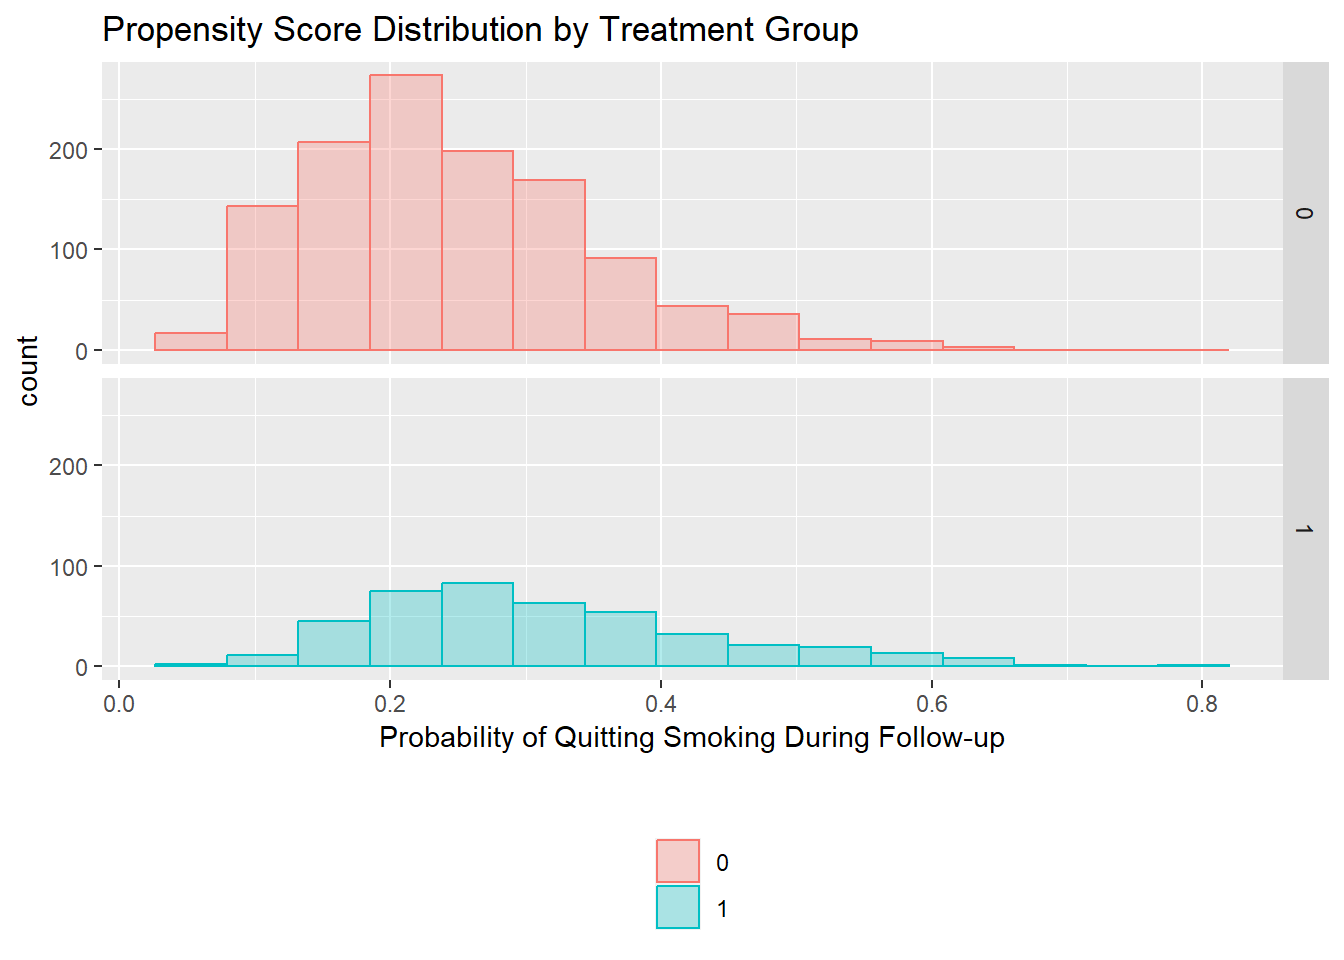
\includegraphics[width=0.85\linewidth]{15-prop-scores-r_files/figure-latex/unnamed-chunk-3-2} \end{center}

\begin{Shaded}
\begin{Highlighting}[]
\CommentTok{\# attempt to reproduce plot from the book}
\NormalTok{nhefs }\SpecialCharTok{\%\textgreater{}\%}
  \FunctionTok{mutate}\NormalTok{(}\AttributeTok{ps.grp =} \FunctionTok{round}\NormalTok{(ps}\SpecialCharTok{/}\FloatTok{0.05}\NormalTok{) }\SpecialCharTok{*} \FloatTok{0.05}\NormalTok{) }\SpecialCharTok{\%\textgreater{}\%}
  \FunctionTok{group\_by}\NormalTok{(qsmk, ps.grp) }\SpecialCharTok{\%\textgreater{}\%}
  \FunctionTok{summarize}\NormalTok{(}\AttributeTok{n =} \FunctionTok{n}\NormalTok{()) }\SpecialCharTok{\%\textgreater{}\%}
  \FunctionTok{ungroup}\NormalTok{() }\SpecialCharTok{\%\textgreater{}\%}
  \FunctionTok{mutate}\NormalTok{(}\AttributeTok{n2 =} \FunctionTok{ifelse}\NormalTok{(qsmk }\SpecialCharTok{==} \DecValTok{0}\NormalTok{, }\AttributeTok{yes =}\NormalTok{ n, }\AttributeTok{no =}  \SpecialCharTok{{-}}\DecValTok{1}\SpecialCharTok{*}\NormalTok{n)) }\SpecialCharTok{\%\textgreater{}\%}
  \FunctionTok{ggplot}\NormalTok{(}\FunctionTok{aes}\NormalTok{(}\AttributeTok{x =}\NormalTok{ ps.grp, }\AttributeTok{y =}\NormalTok{ n2, }\AttributeTok{fill =} \FunctionTok{as.factor}\NormalTok{(qsmk))) }\SpecialCharTok{+}
  \FunctionTok{geom\_bar}\NormalTok{(}\AttributeTok{stat =} \StringTok{\textquotesingle{}identity\textquotesingle{}}\NormalTok{, }\AttributeTok{position =} \StringTok{\textquotesingle{}identity\textquotesingle{}}\NormalTok{) }\SpecialCharTok{+}
  \FunctionTok{geom\_text}\NormalTok{(}\FunctionTok{aes}\NormalTok{(}\AttributeTok{label =}\NormalTok{ n, }\AttributeTok{x =}\NormalTok{ ps.grp, }\AttributeTok{y =}\NormalTok{ n2 }\SpecialCharTok{+} \FunctionTok{ifelse}\NormalTok{(qsmk }\SpecialCharTok{==} \DecValTok{0}\NormalTok{, }\DecValTok{8}\NormalTok{, }\SpecialCharTok{{-}}\DecValTok{8}\NormalTok{))) }\SpecialCharTok{+}
  \FunctionTok{xlab}\NormalTok{(}\StringTok{\textquotesingle{}Probability of Quitting Smoking During Follow{-}up\textquotesingle{}}\NormalTok{) }\SpecialCharTok{+}
  \FunctionTok{ylab}\NormalTok{(}\StringTok{\textquotesingle{}N\textquotesingle{}}\NormalTok{) }\SpecialCharTok{+}
  \FunctionTok{ggtitle}\NormalTok{(}\StringTok{\textquotesingle{}Propensity Score Distribution by Treatment Group\textquotesingle{}}\NormalTok{) }\SpecialCharTok{+}
  \FunctionTok{scale\_fill\_discrete}\NormalTok{(}\StringTok{\textquotesingle{}\textquotesingle{}}\NormalTok{) }\SpecialCharTok{+}
  \FunctionTok{scale\_x\_continuous}\NormalTok{(}\AttributeTok{breaks =} \FunctionTok{seq}\NormalTok{(}\DecValTok{0}\NormalTok{, }\DecValTok{1}\NormalTok{, }\FloatTok{0.05}\NormalTok{)) }\SpecialCharTok{+}
  \FunctionTok{theme}\NormalTok{(}\AttributeTok{legend.position =} \StringTok{\textquotesingle{}bottom\textquotesingle{}}\NormalTok{, }\AttributeTok{legend.direction =} \StringTok{\textquotesingle{}vertical\textquotesingle{}}\NormalTok{,}
        \AttributeTok{axis.ticks.y =} \FunctionTok{element\_blank}\NormalTok{(),}
        \AttributeTok{axis.text.y =} \FunctionTok{element\_blank}\NormalTok{())}
\end{Highlighting}
\end{Shaded}

\hypertarget{program-15.3}{%
\section{Program 15.3}\label{program-15.3}}

\begin{itemize}
\tightlist
\item
  Stratification on the propensity score
\item
  Data from NHEFS
\end{itemize}

\begin{Shaded}
\begin{Highlighting}[]
\CommentTok{\# calculation of deciles}
\NormalTok{nhefs}\SpecialCharTok{$}\NormalTok{ps.dec }\OtherTok{\textless{}{-}} \FunctionTok{cut}\NormalTok{(nhefs}\SpecialCharTok{$}\NormalTok{ps, }
                    \AttributeTok{breaks=}\FunctionTok{c}\NormalTok{(}\FunctionTok{quantile}\NormalTok{(nhefs}\SpecialCharTok{$}\NormalTok{ps, }\AttributeTok{probs=}\FunctionTok{seq}\NormalTok{(}\DecValTok{0}\NormalTok{,}\DecValTok{1}\NormalTok{,}\FloatTok{0.1}\NormalTok{))),}
                    \AttributeTok{labels=}\FunctionTok{seq}\NormalTok{(}\DecValTok{1}\SpecialCharTok{:}\DecValTok{10}\NormalTok{),}
                    \AttributeTok{include.lowest=}\ConstantTok{TRUE}\NormalTok{)}

\CommentTok{\#install.packages("psych") \# install package if required}
\FunctionTok{library}\NormalTok{(}\StringTok{"psych"}\NormalTok{)}
\end{Highlighting}
\end{Shaded}

\begin{verbatim}
## 
## Attaching package: 'psych'
\end{verbatim}

\begin{verbatim}
## The following objects are masked from 'package:ggplot2':
## 
##     %+%, alpha
\end{verbatim}

\begin{Shaded}
\begin{Highlighting}[]
\FunctionTok{describeBy}\NormalTok{(nhefs}\SpecialCharTok{$}\NormalTok{ps, }\FunctionTok{list}\NormalTok{(nhefs}\SpecialCharTok{$}\NormalTok{ps.dec, nhefs}\SpecialCharTok{$}\NormalTok{qsmk))}
\end{Highlighting}
\end{Shaded}

\begin{verbatim}
## 
##  Descriptive statistics by group 
## : 1
## : 0
##    vars   n mean   sd median trimmed  mad  min  max range  skew kurtosis se
## X1    1 151  0.1 0.02   0.11     0.1 0.02 0.05 0.13  0.08 -0.55    -0.53  0
## ------------------------------------------------------------ 
## : 2
## : 0
##    vars   n mean   sd median trimmed  mad  min  max range  skew kurtosis se
## X1    1 136 0.15 0.01   0.15    0.15 0.01 0.13 0.17  0.04 -0.04    -1.23  0
## ------------------------------------------------------------ 
## : 3
## : 0
##    vars   n mean   sd median trimmed  mad  min  max range  skew kurtosis se
## X1    1 134 0.18 0.01   0.18    0.18 0.01 0.17 0.19  0.03 -0.08    -1.34  0
## ------------------------------------------------------------ 
## : 4
## : 0
##    vars   n mean   sd median trimmed  mad  min  max range  skew kurtosis se
## X1    1 129 0.21 0.01   0.21    0.21 0.01 0.19 0.22  0.02 -0.04    -1.13  0
## ------------------------------------------------------------ 
## : 5
## : 0
##    vars   n mean   sd median trimmed  mad  min  max range skew kurtosis se
## X1    1 120 0.23 0.01   0.23    0.23 0.01 0.22 0.25  0.03 0.24    -1.22  0
## ------------------------------------------------------------ 
## : 6
## : 0
##    vars   n mean   sd median trimmed  mad  min  max range  skew kurtosis se
## X1    1 117 0.26 0.01   0.26    0.26 0.01 0.25 0.27  0.03 -0.11    -1.29  0
## ------------------------------------------------------------ 
## : 7
## : 0
##    vars   n mean   sd median trimmed  mad  min  max range  skew kurtosis se
## X1    1 120 0.29 0.01   0.29    0.29 0.01 0.27 0.31  0.03 -0.23    -1.19  0
## ------------------------------------------------------------ 
## : 8
## : 0
##    vars   n mean   sd median trimmed  mad  min  max range skew kurtosis se
## X1    1 112 0.33 0.01   0.33    0.33 0.02 0.31 0.35  0.04 0.15     -1.1  0
## ------------------------------------------------------------ 
## : 9
## : 0
##    vars  n mean   sd median trimmed  mad  min  max range skew kurtosis se
## X1    1 96 0.38 0.02   0.38    0.38 0.02 0.35 0.42  0.06 0.13    -1.15  0
## ------------------------------------------------------------ 
## : 10
## : 0
##    vars  n mean   sd median trimmed  mad  min  max range skew kurtosis   se
## X1    1 86 0.49 0.06   0.47    0.48 0.05 0.42 0.66  0.24  1.1     0.47 0.01
## ------------------------------------------------------------ 
## : 1
## : 1
##    vars  n mean   sd median trimmed  mad  min  max range skew kurtosis   se
## X1    1 12  0.1 0.02   0.11     0.1 0.03 0.06 0.13  0.07 -0.5    -1.36 0.01
## ------------------------------------------------------------ 
## : 2
## : 1
##    vars  n mean   sd median trimmed  mad  min  max range  skew kurtosis se
## X1    1 27 0.15 0.01   0.15    0.15 0.01 0.13 0.17  0.03 -0.03    -1.34  0
## ------------------------------------------------------------ 
## : 3
## : 1
##    vars  n mean   sd median trimmed  mad  min  max range skew kurtosis se
## X1    1 29 0.18 0.01   0.18    0.18 0.01 0.17 0.19  0.03 0.01    -1.34  0
## ------------------------------------------------------------ 
## : 4
## : 1
##    vars  n mean   sd median trimmed  mad  min  max range  skew kurtosis se
## X1    1 34 0.21 0.01   0.21    0.21 0.01 0.19 0.22  0.02 -0.31    -1.23  0
## ------------------------------------------------------------ 
## : 5
## : 1
##    vars  n mean   sd median trimmed  mad  min  max range skew kurtosis se
## X1    1 43 0.23 0.01   0.23    0.23 0.01 0.22 0.25  0.03 0.11    -1.23  0
## ------------------------------------------------------------ 
## : 6
## : 1
##    vars  n mean   sd median trimmed  mad  min  max range skew kurtosis se
## X1    1 45 0.26 0.01   0.26    0.26 0.01 0.25 0.27  0.03  0.2    -1.12  0
## ------------------------------------------------------------ 
## : 7
## : 1
##    vars  n mean   sd median trimmed  mad  min  max range skew kurtosis se
## X1    1 43 0.29 0.01   0.29    0.29 0.01 0.27 0.31  0.03 0.16    -1.25  0
## ------------------------------------------------------------ 
## : 8
## : 1
##    vars  n mean   sd median trimmed  mad  min  max range skew kurtosis se
## X1    1 51 0.33 0.01   0.33    0.33 0.02 0.31 0.35  0.04 0.11    -1.19  0
## ------------------------------------------------------------ 
## : 9
## : 1
##    vars  n mean   sd median trimmed  mad  min  max range skew kurtosis se
## X1    1 67 0.38 0.02   0.38    0.38 0.03 0.35 0.42  0.06 0.19    -1.27  0
## ------------------------------------------------------------ 
## : 10
## : 1
##    vars  n mean   sd median trimmed  mad  min  max range skew kurtosis   se
## X1    1 77 0.52 0.08   0.51    0.51 0.08 0.42 0.79  0.38 0.88     0.81 0.01
\end{verbatim}

\begin{Shaded}
\begin{Highlighting}[]
\CommentTok{\# function to create deciles easily}
\NormalTok{decile }\OtherTok{\textless{}{-}} \ControlFlowTok{function}\NormalTok{(x) \{}
  \FunctionTok{return}\NormalTok{(}\FunctionTok{factor}\NormalTok{(}\FunctionTok{quantcut}\NormalTok{(x, }\FunctionTok{seq}\NormalTok{(}\DecValTok{0}\NormalTok{, }\DecValTok{1}\NormalTok{, }\FloatTok{0.1}\NormalTok{), }\AttributeTok{labels =} \ConstantTok{FALSE}\NormalTok{)))}
\NormalTok{\}}

\CommentTok{\# regression on PS deciles, allowing for effect modification}
\ControlFlowTok{for}\NormalTok{ (deciles }\ControlFlowTok{in} \FunctionTok{c}\NormalTok{(}\DecValTok{1}\SpecialCharTok{:}\DecValTok{10}\NormalTok{)) \{}
  \FunctionTok{print}\NormalTok{(}\FunctionTok{t.test}\NormalTok{(wt82\_71}\SpecialCharTok{\textasciitilde{}}\NormalTok{qsmk, }\AttributeTok{data=}\NormalTok{nhefs[}\FunctionTok{which}\NormalTok{(nhefs}\SpecialCharTok{$}\NormalTok{ps.dec}\SpecialCharTok{==}\NormalTok{deciles),]))}
\NormalTok{\}}
\end{Highlighting}
\end{Shaded}

\begin{verbatim}
## 
##  Welch Two Sample t-test
## 
## data:  wt82_71 by qsmk
## t = 0.0060506, df = 11.571, p-value = 0.9953
## alternative hypothesis: true difference in means between group 0 and group 1 is not equal to 0
## 95 percent confidence interval:
##  -5.283903  5.313210
## sample estimates:
## mean in group 0 mean in group 1 
##        3.995205        3.980551 
## 
## 
##  Welch Two Sample t-test
## 
## data:  wt82_71 by qsmk
## t = -3.1117, df = 37.365, p-value = 0.003556
## alternative hypothesis: true difference in means between group 0 and group 1 is not equal to 0
## 95 percent confidence interval:
##  -6.849335 -1.448161
## sample estimates:
## mean in group 0 mean in group 1 
##        2.904679        7.053426 
## 
## 
##  Welch Two Sample t-test
## 
## data:  wt82_71 by qsmk
## t = -4.5301, df = 35.79, p-value = 6.317e-05
## alternative hypothesis: true difference in means between group 0 and group 1 is not equal to 0
## 95 percent confidence interval:
##  -9.474961 -3.613990
## sample estimates:
## mean in group 0 mean in group 1 
##        2.612094        9.156570 
## 
## 
##  Welch Two Sample t-test
## 
## data:  wt82_71 by qsmk
## t = -1.4117, df = 45.444, p-value = 0.1648
## alternative hypothesis: true difference in means between group 0 and group 1 is not equal to 0
## 95 percent confidence interval:
##  -5.6831731  0.9985715
## sample estimates:
## mean in group 0 mean in group 1 
##        3.474679        5.816979 
## 
## 
##  Welch Two Sample t-test
## 
## data:  wt82_71 by qsmk
## t = -3.1371, df = 74.249, p-value = 0.002446
## alternative hypothesis: true difference in means between group 0 and group 1 is not equal to 0
## 95 percent confidence interval:
##  -6.753621 -1.507087
## sample estimates:
## mean in group 0 mean in group 1 
##        2.098800        6.229154 
## 
## 
##  Welch Two Sample t-test
## 
## data:  wt82_71 by qsmk
## t = -2.1677, df = 50.665, p-value = 0.0349
## alternative hypothesis: true difference in means between group 0 and group 1 is not equal to 0
## 95 percent confidence interval:
##  -8.7516605 -0.3350127
## sample estimates:
## mean in group 0 mean in group 1 
##        1.847004        6.390340 
## 
## 
##  Welch Two Sample t-test
## 
## data:  wt82_71 by qsmk
## t = -3.3155, df = 84.724, p-value = 0.001348
## alternative hypothesis: true difference in means between group 0 and group 1 is not equal to 0
## 95 percent confidence interval:
##  -6.904207 -1.727590
## sample estimates:
## mean in group 0 mean in group 1 
##        1.560048        5.875946 
## 
## 
##  Welch Two Sample t-test
## 
## data:  wt82_71 by qsmk
## t = -2.664, df = 75.306, p-value = 0.009441
## alternative hypothesis: true difference in means between group 0 and group 1 is not equal to 0
## 95 percent confidence interval:
##  -6.2396014 -0.9005605
## sample estimates:
## mean in group 0 mean in group 1 
##       0.2846851       3.8547661 
## 
## 
##  Welch Two Sample t-test
## 
## data:  wt82_71 by qsmk
## t = -1.9122, df = 129.12, p-value = 0.05806
## alternative hypothesis: true difference in means between group 0 and group 1 is not equal to 0
## 95 percent confidence interval:
##  -4.68143608  0.07973698
## sample estimates:
## mean in group 0 mean in group 1 
##      -0.8954482       1.4054014 
## 
## 
##  Welch Two Sample t-test
## 
## data:  wt82_71 by qsmk
## t = -1.5925, df = 142.72, p-value = 0.1135
## alternative hypothesis: true difference in means between group 0 and group 1 is not equal to 0
## 95 percent confidence interval:
##  -5.0209284  0.5404697
## sample estimates:
## mean in group 0 mean in group 1 
##      -0.5043766       1.7358528
\end{verbatim}

\begin{Shaded}
\begin{Highlighting}[]
\CommentTok{\# regression on PS deciles, not allowing for effect modification}
\NormalTok{fit.psdec }\OtherTok{\textless{}{-}} \FunctionTok{glm}\NormalTok{(wt82\_71 }\SpecialCharTok{\textasciitilde{}}\NormalTok{ qsmk }\SpecialCharTok{+} \FunctionTok{as.factor}\NormalTok{(ps.dec), }\AttributeTok{data =}\NormalTok{ nhefs)}
\FunctionTok{summary}\NormalTok{(fit.psdec)}
\end{Highlighting}
\end{Shaded}

\begin{verbatim}
## 
## Call:
## glm(formula = wt82_71 ~ qsmk + as.factor(ps.dec), data = nhefs)
## 
## Deviance Residuals: 
##     Min       1Q   Median       3Q      Max  
## -43.543   -3.932   -0.085    4.233   46.773  
## 
## Coefficients:
##                     Estimate Std. Error t value Pr(>|t|)    
## (Intercept)           3.7505     0.6089   6.159 9.29e-10 ***
## qsmk                  3.5005     0.4571   7.659 3.28e-14 ***
## as.factor(ps.dec)2   -0.7391     0.8611  -0.858   0.3908    
## as.factor(ps.dec)3   -0.6182     0.8612  -0.718   0.4730    
## as.factor(ps.dec)4   -0.5204     0.8584  -0.606   0.5444    
## as.factor(ps.dec)5   -1.4884     0.8590  -1.733   0.0834 .  
## as.factor(ps.dec)6   -1.6227     0.8675  -1.871   0.0616 .  
## as.factor(ps.dec)7   -1.9853     0.8681  -2.287   0.0223 *  
## as.factor(ps.dec)8   -3.4447     0.8749  -3.937 8.61e-05 ***
## as.factor(ps.dec)9   -5.1544     0.8848  -5.825 6.91e-09 ***
## as.factor(ps.dec)10  -4.8403     0.8828  -5.483 4.87e-08 ***
## ---
## Signif. codes:  0 '***' 0.001 '**' 0.01 '*' 0.05 '.' 0.1 ' ' 1
## 
## (Dispersion parameter for gaussian family taken to be 58.42297)
## 
##     Null deviance: 97176  on 1565  degrees of freedom
## Residual deviance: 90848  on 1555  degrees of freedom
##   (63 observations deleted due to missingness)
## AIC: 10827
## 
## Number of Fisher Scoring iterations: 2
\end{verbatim}

\begin{Shaded}
\begin{Highlighting}[]
\FunctionTok{confint.lm}\NormalTok{(fit.psdec)}
\end{Highlighting}
\end{Shaded}

\begin{verbatim}
##                         2.5 %      97.5 %
## (Intercept)          2.556098  4.94486263
## qsmk                 2.603953  4.39700504
## as.factor(ps.dec)2  -2.428074  0.94982494
## as.factor(ps.dec)3  -2.307454  1.07103569
## as.factor(ps.dec)4  -2.204103  1.16333143
## as.factor(ps.dec)5  -3.173337  0.19657938
## as.factor(ps.dec)6  -3.324345  0.07893027
## as.factor(ps.dec)7  -3.688043 -0.28248110
## as.factor(ps.dec)8  -5.160862 -1.72860113
## as.factor(ps.dec)9  -6.889923 -3.41883853
## as.factor(ps.dec)10 -6.571789 -3.10873731
\end{verbatim}

\hypertarget{program-15.4}{%
\section{Program 15.4}\label{program-15.4}}

\begin{itemize}
\tightlist
\item
  Standardization using the propensity score
\item
  Data from NHEFS
\end{itemize}

\begin{Shaded}
\begin{Highlighting}[]
\CommentTok{\#install.packages("boot") \# install package if required}
\FunctionTok{library}\NormalTok{(}\StringTok{"boot"}\NormalTok{)}
\end{Highlighting}
\end{Shaded}

\begin{verbatim}
## 
## Attaching package: 'boot'
\end{verbatim}

\begin{verbatim}
## The following object is masked from 'package:psych':
## 
##     logit
\end{verbatim}

\begin{verbatim}
## The following object is masked from 'package:survival':
## 
##     aml
\end{verbatim}

\begin{Shaded}
\begin{Highlighting}[]
\CommentTok{\# standardization by propensity score, agnostic regarding effect modification }
\NormalTok{std.ps }\OtherTok{\textless{}{-}} \ControlFlowTok{function}\NormalTok{(data, indices) \{}
\NormalTok{  d }\OtherTok{\textless{}{-}}\NormalTok{ data[indices,] }\CommentTok{\# 1st copy: equal to original one\textasciigrave{}}
  \CommentTok{\# calculating propensity scores}
\NormalTok{  ps.fit }\OtherTok{\textless{}{-}} \FunctionTok{glm}\NormalTok{(qsmk }\SpecialCharTok{\textasciitilde{}}\NormalTok{ sex }\SpecialCharTok{+}\NormalTok{ race }\SpecialCharTok{+}\NormalTok{ age }\SpecialCharTok{+} \FunctionTok{I}\NormalTok{(age}\SpecialCharTok{*}\NormalTok{age) }
                \SpecialCharTok{+} \FunctionTok{as.factor}\NormalTok{(education) }\SpecialCharTok{+}\NormalTok{ smokeintensity}
                \SpecialCharTok{+} \FunctionTok{I}\NormalTok{(smokeintensity}\SpecialCharTok{*}\NormalTok{smokeintensity) }\SpecialCharTok{+}\NormalTok{ smokeyrs}
                \SpecialCharTok{+} \FunctionTok{I}\NormalTok{(smokeyrs}\SpecialCharTok{*}\NormalTok{smokeyrs) }\SpecialCharTok{+} \FunctionTok{as.factor}\NormalTok{(exercise)}
                \SpecialCharTok{+} \FunctionTok{as.factor}\NormalTok{(active) }\SpecialCharTok{+}\NormalTok{ wt71 }\SpecialCharTok{+} \FunctionTok{I}\NormalTok{(wt71}\SpecialCharTok{*}\NormalTok{wt71),}
                \AttributeTok{data=}\NormalTok{d, }\AttributeTok{family=}\FunctionTok{binomial}\NormalTok{())}
\NormalTok{  d}\SpecialCharTok{$}\NormalTok{pscore }\OtherTok{\textless{}{-}} \FunctionTok{predict}\NormalTok{(ps.fit, d, }\AttributeTok{type=}\StringTok{"response"}\NormalTok{)}
  
  \CommentTok{\# create a dataset with 3 copies of each subject}
\NormalTok{  d}\SpecialCharTok{$}\NormalTok{interv }\OtherTok{\textless{}{-}} \SpecialCharTok{{-}}\DecValTok{1} \CommentTok{\# 1st copy: equal to original one\textasciigrave{}}
\NormalTok{  d0 }\OtherTok{\textless{}{-}}\NormalTok{ d }\CommentTok{\# 2nd copy: treatment set to 0, outcome to missing}
\NormalTok{  d0}\SpecialCharTok{$}\NormalTok{interv }\OtherTok{\textless{}{-}} \DecValTok{0}
\NormalTok{  d0}\SpecialCharTok{$}\NormalTok{qsmk }\OtherTok{\textless{}{-}} \DecValTok{0}
\NormalTok{  d0}\SpecialCharTok{$}\NormalTok{wt82\_71 }\OtherTok{\textless{}{-}} \ConstantTok{NA}
\NormalTok{  d1 }\OtherTok{\textless{}{-}}\NormalTok{ d }\CommentTok{\# 3rd copy: treatment set to 1, outcome to missing}
\NormalTok{  d1}\SpecialCharTok{$}\NormalTok{interv }\OtherTok{\textless{}{-}} \DecValTok{1}
\NormalTok{  d1}\SpecialCharTok{$}\NormalTok{qsmk }\OtherTok{\textless{}{-}} \DecValTok{1}
\NormalTok{  d1}\SpecialCharTok{$}\NormalTok{wt82\_71 }\OtherTok{\textless{}{-}} \ConstantTok{NA}
\NormalTok{  d.onesample }\OtherTok{\textless{}{-}} \FunctionTok{rbind}\NormalTok{(d, d0, d1) }\CommentTok{\# combining datasets}

\NormalTok{  std.fit }\OtherTok{\textless{}{-}} \FunctionTok{glm}\NormalTok{(wt82\_71 }\SpecialCharTok{\textasciitilde{}}\NormalTok{ qsmk }\SpecialCharTok{+}\NormalTok{ pscore }\SpecialCharTok{+} \FunctionTok{I}\NormalTok{(qsmk}\SpecialCharTok{*}\NormalTok{pscore), }\AttributeTok{data=}\NormalTok{d.onesample)}
\NormalTok{  d.onesample}\SpecialCharTok{$}\NormalTok{predicted\_meanY }\OtherTok{\textless{}{-}} \FunctionTok{predict}\NormalTok{(std.fit, d.onesample)}

  \CommentTok{\# estimate mean outcome in each of the groups interv={-}1, interv=0, and interv=1}
  \FunctionTok{return}\NormalTok{(}\FunctionTok{c}\NormalTok{(}\FunctionTok{mean}\NormalTok{(d.onesample}\SpecialCharTok{$}\NormalTok{predicted\_meanY[d.onesample}\SpecialCharTok{$}\NormalTok{interv}\SpecialCharTok{=={-}}\DecValTok{1}\NormalTok{]),}
           \FunctionTok{mean}\NormalTok{(d.onesample}\SpecialCharTok{$}\NormalTok{predicted\_meanY[d.onesample}\SpecialCharTok{$}\NormalTok{interv}\SpecialCharTok{==}\DecValTok{0}\NormalTok{]),}
           \FunctionTok{mean}\NormalTok{(d.onesample}\SpecialCharTok{$}\NormalTok{predicted\_meanY[d.onesample}\SpecialCharTok{$}\NormalTok{interv}\SpecialCharTok{==}\DecValTok{1}\NormalTok{]),}
           \FunctionTok{mean}\NormalTok{(d.onesample}\SpecialCharTok{$}\NormalTok{predicted\_meanY[d.onesample}\SpecialCharTok{$}\NormalTok{interv}\SpecialCharTok{==}\DecValTok{1}\NormalTok{])}\SpecialCharTok{{-}}
             \FunctionTok{mean}\NormalTok{(d.onesample}\SpecialCharTok{$}\NormalTok{predicted\_meanY[d.onesample}\SpecialCharTok{$}\NormalTok{interv}\SpecialCharTok{==}\DecValTok{0}\NormalTok{])))}
\NormalTok{\}}

\CommentTok{\# bootstrap}
\NormalTok{results }\OtherTok{\textless{}{-}} \FunctionTok{boot}\NormalTok{(}\AttributeTok{data=}\NormalTok{nhefs, }\AttributeTok{statistic=}\NormalTok{std.ps, }\AttributeTok{R=}\DecValTok{5}\NormalTok{)}

\CommentTok{\# generating confidence intervals}
\NormalTok{se }\OtherTok{\textless{}{-}} \FunctionTok{c}\NormalTok{(}\FunctionTok{sd}\NormalTok{(results}\SpecialCharTok{$}\NormalTok{t[,}\DecValTok{1}\NormalTok{]), }\FunctionTok{sd}\NormalTok{(results}\SpecialCharTok{$}\NormalTok{t[,}\DecValTok{2}\NormalTok{]), }
        \FunctionTok{sd}\NormalTok{(results}\SpecialCharTok{$}\NormalTok{t[,}\DecValTok{3}\NormalTok{]), }\FunctionTok{sd}\NormalTok{(results}\SpecialCharTok{$}\NormalTok{t[,}\DecValTok{4}\NormalTok{]))}
\NormalTok{mean }\OtherTok{\textless{}{-}}\NormalTok{ results}\SpecialCharTok{$}\NormalTok{t0}
\NormalTok{ll }\OtherTok{\textless{}{-}}\NormalTok{ mean }\SpecialCharTok{{-}} \FunctionTok{qnorm}\NormalTok{(}\FloatTok{0.975}\NormalTok{)}\SpecialCharTok{*}\NormalTok{se}
\NormalTok{ul }\OtherTok{\textless{}{-}}\NormalTok{ mean }\SpecialCharTok{+} \FunctionTok{qnorm}\NormalTok{(}\FloatTok{0.975}\NormalTok{)}\SpecialCharTok{*}\NormalTok{se}

\NormalTok{bootstrap }\OtherTok{\textless{}{-}} \FunctionTok{data.frame}\NormalTok{(}\FunctionTok{cbind}\NormalTok{(}\FunctionTok{c}\NormalTok{(}\StringTok{"Observed"}\NormalTok{, }\StringTok{"No Treatment"}\NormalTok{, }\StringTok{"Treatment"}\NormalTok{, }
                                \StringTok{"Treatment {-} No Treatment"}\NormalTok{), mean, se, ll, ul))}
\NormalTok{bootstrap}
\end{Highlighting}
\end{Shaded}

\begin{verbatim}
##                         V1             mean                se               ll
## 1                 Observed 2.63384609228479 0.133091272063885 2.37299199238296
## 2             No Treatment 1.71983636149843 0.154133540347683 1.41774017360731
## 3                Treatment 5.35072300362993  0.49183904096712 4.38673619714365
## 4 Treatment - No Treatment  3.6308866421315 0.521358399748788 2.60904295558644
##                 ul
## 1 2.89470019218663
## 2 2.02193254938954
## 3  6.3147098101162
## 4 4.65273032867656
\end{verbatim}

\begin{Shaded}
\begin{Highlighting}[]
\CommentTok{\# regression on the propensity score (linear term)}
\NormalTok{model6 }\OtherTok{\textless{}{-}} \FunctionTok{glm}\NormalTok{(wt82\_71 }\SpecialCharTok{\textasciitilde{}}\NormalTok{ qsmk }\SpecialCharTok{+}\NormalTok{ ps, }\AttributeTok{data =}\NormalTok{ nhefs) }\CommentTok{\# p.qsmk}
\FunctionTok{summary}\NormalTok{(model6)}
\end{Highlighting}
\end{Shaded}

\begin{verbatim}
## 
## Call:
## glm(formula = wt82_71 ~ qsmk + ps, data = nhefs)
## 
## Deviance Residuals: 
##     Min       1Q   Median       3Q      Max  
## -43.314   -4.006   -0.068    4.244   47.158  
## 
## Coefficients:
##             Estimate Std. Error t value Pr(>|t|)    
## (Intercept)   5.5945     0.4831  11.581  < 2e-16 ***
## qsmk          3.5506     0.4573   7.765 1.47e-14 ***
## ps          -14.8218     1.7576  -8.433  < 2e-16 ***
## ---
## Signif. codes:  0 '***' 0.001 '**' 0.01 '*' 0.05 '.' 0.1 ' ' 1
## 
## (Dispersion parameter for gaussian family taken to be 58.28455)
## 
##     Null deviance: 97176  on 1565  degrees of freedom
## Residual deviance: 91099  on 1563  degrees of freedom
##   (63 observations deleted due to missingness)
## AIC: 10815
## 
## Number of Fisher Scoring iterations: 2
\end{verbatim}

\begin{Shaded}
\begin{Highlighting}[]
\CommentTok{\# standarization on the propensity score}
\CommentTok{\# (step 1) create two new datasets, one with all treated and one with all untreated}
\NormalTok{treated }\OtherTok{\textless{}{-}}\NormalTok{ nhefs}
\NormalTok{  treated}\SpecialCharTok{$}\NormalTok{qsmk }\OtherTok{\textless{}{-}} \DecValTok{1}

\NormalTok{untreated }\OtherTok{\textless{}{-}}\NormalTok{ nhefs}
\NormalTok{  untreated}\SpecialCharTok{$}\NormalTok{qsmk }\OtherTok{\textless{}{-}} \DecValTok{0}

\CommentTok{\# (step 2) predict values for everyone in each new dataset based on above model}
\NormalTok{treated}\SpecialCharTok{$}\NormalTok{pred.y }\OtherTok{\textless{}{-}} \FunctionTok{predict}\NormalTok{(model6, treated)}
\NormalTok{untreated}\SpecialCharTok{$}\NormalTok{pred.y }\OtherTok{\textless{}{-}} \FunctionTok{predict}\NormalTok{(model6, untreated)}

\CommentTok{\# (step 3) compare mean weight loss had all been treated vs. that had all been untreated}
\NormalTok{mean1 }\OtherTok{\textless{}{-}} \FunctionTok{mean}\NormalTok{(treated}\SpecialCharTok{$}\NormalTok{pred.y, }\AttributeTok{na.rm =} \ConstantTok{TRUE}\NormalTok{)}
\NormalTok{mean0 }\OtherTok{\textless{}{-}} \FunctionTok{mean}\NormalTok{(untreated}\SpecialCharTok{$}\NormalTok{pred.y, }\AttributeTok{na.rm =} \ConstantTok{TRUE}\NormalTok{)}
\NormalTok{mean1}
\end{Highlighting}
\end{Shaded}

\begin{verbatim}
## [1] 5.250824
\end{verbatim}

\begin{Shaded}
\begin{Highlighting}[]
\NormalTok{mean0}
\end{Highlighting}
\end{Shaded}

\begin{verbatim}
## [1] 1.700228
\end{verbatim}

\begin{Shaded}
\begin{Highlighting}[]
\NormalTok{mean1 }\SpecialCharTok{{-}}\NormalTok{ mean0}
\end{Highlighting}
\end{Shaded}

\begin{verbatim}
## [1] 3.550596
\end{verbatim}

\begin{Shaded}
\begin{Highlighting}[]
\CommentTok{\# (step 4) bootstrap a confidence interval}
\CommentTok{\# number of bootstraps}
\NormalTok{nboot }\OtherTok{\textless{}{-}} \DecValTok{100}
\CommentTok{\# set up a matrix to store results}
\NormalTok{boots }\OtherTok{\textless{}{-}} \FunctionTok{data.frame}\NormalTok{(}\AttributeTok{i =} \DecValTok{1}\SpecialCharTok{:}\NormalTok{nboot,}
                    \AttributeTok{mean1 =} \ConstantTok{NA}\NormalTok{,}
                    \AttributeTok{mean0 =} \ConstantTok{NA}\NormalTok{,}
                    \AttributeTok{difference =} \ConstantTok{NA}\NormalTok{)}
\CommentTok{\# loop to perform the bootstrapping}
\NormalTok{nhefs }\OtherTok{\textless{}{-}} \FunctionTok{subset}\NormalTok{(nhefs, }\SpecialCharTok{!}\FunctionTok{is.na}\NormalTok{(ps) }\SpecialCharTok{\&} \SpecialCharTok{!}\FunctionTok{is.na}\NormalTok{(wt82\_71)) }\CommentTok{\# p.qsmk}
\ControlFlowTok{for}\NormalTok{(i }\ControlFlowTok{in} \DecValTok{1}\SpecialCharTok{:}\NormalTok{nboot) \{}
  \CommentTok{\# sample with replacement}
\NormalTok{  sampl }\OtherTok{\textless{}{-}}\NormalTok{ nhefs[}\FunctionTok{sample}\NormalTok{(}\DecValTok{1}\SpecialCharTok{:}\FunctionTok{nrow}\NormalTok{(nhefs), }\FunctionTok{nrow}\NormalTok{(nhefs), }\AttributeTok{replace =} \ConstantTok{TRUE}\NormalTok{), ]}
  
  \CommentTok{\# fit the model in the bootstrap sample}
\NormalTok{  bootmod }\OtherTok{\textless{}{-}} \FunctionTok{glm}\NormalTok{(wt82\_71 }\SpecialCharTok{\textasciitilde{}}\NormalTok{ qsmk }\SpecialCharTok{+}\NormalTok{ ps, }\AttributeTok{data =}\NormalTok{ sampl) }\CommentTok{\# ps}
  
  \CommentTok{\# create new datasets}
\NormalTok{  sampl.treated }\OtherTok{\textless{}{-}}\NormalTok{ sampl }\SpecialCharTok{\%\textgreater{}\%}
    \FunctionTok{mutate}\NormalTok{(}\AttributeTok{qsmk =} \DecValTok{1}\NormalTok{)}
  
\NormalTok{  sampl.untreated }\OtherTok{\textless{}{-}}\NormalTok{ sampl }\SpecialCharTok{\%\textgreater{}\%}
    \FunctionTok{mutate}\NormalTok{(}\AttributeTok{qsmk =} \DecValTok{0}\NormalTok{)}
  
  \CommentTok{\# predict values}
\NormalTok{  sampl.treated}\SpecialCharTok{$}\NormalTok{pred.y }\OtherTok{\textless{}{-}} \FunctionTok{predict}\NormalTok{(bootmod, sampl.treated)}
\NormalTok{  sampl.untreated}\SpecialCharTok{$}\NormalTok{pred.y }\OtherTok{\textless{}{-}} \FunctionTok{predict}\NormalTok{(bootmod, sampl.untreated)}
  
  \CommentTok{\# output results }
\NormalTok{  boots[i, }\StringTok{\textquotesingle{}mean1\textquotesingle{}}\NormalTok{] }\OtherTok{\textless{}{-}} \FunctionTok{mean}\NormalTok{(sampl.treated}\SpecialCharTok{$}\NormalTok{pred.y, }\AttributeTok{na.rm =} \ConstantTok{TRUE}\NormalTok{)}
\NormalTok{  boots[i, }\StringTok{\textquotesingle{}mean0\textquotesingle{}}\NormalTok{] }\OtherTok{\textless{}{-}} \FunctionTok{mean}\NormalTok{(sampl.untreated}\SpecialCharTok{$}\NormalTok{pred.y, }\AttributeTok{na.rm =} \ConstantTok{TRUE}\NormalTok{)}
\NormalTok{  boots[i, }\StringTok{\textquotesingle{}difference\textquotesingle{}}\NormalTok{] }\OtherTok{\textless{}{-}}\NormalTok{ boots[i, }\StringTok{\textquotesingle{}mean1\textquotesingle{}}\NormalTok{] }\SpecialCharTok{{-}}\NormalTok{ boots[i, }\StringTok{\textquotesingle{}mean0\textquotesingle{}}\NormalTok{]}
  
  \CommentTok{\# once loop is done, print the results}
  \ControlFlowTok{if}\NormalTok{(i }\SpecialCharTok{==}\NormalTok{ nboot) \{}
    \FunctionTok{cat}\NormalTok{(}\StringTok{\textquotesingle{}95\% CI for the causal mean difference}\SpecialCharTok{\textbackslash{}n}\StringTok{\textquotesingle{}}\NormalTok{)}
    \FunctionTok{cat}\NormalTok{(}\FunctionTok{mean}\NormalTok{(boots}\SpecialCharTok{$}\NormalTok{difference) }\SpecialCharTok{{-}} \FloatTok{1.96}\SpecialCharTok{*}\FunctionTok{sd}\NormalTok{(boots}\SpecialCharTok{$}\NormalTok{difference), }
        \StringTok{\textquotesingle{},\textquotesingle{}}\NormalTok{,}
        \FunctionTok{mean}\NormalTok{(boots}\SpecialCharTok{$}\NormalTok{difference) }\SpecialCharTok{+} \FloatTok{1.96}\SpecialCharTok{*}\FunctionTok{sd}\NormalTok{(boots}\SpecialCharTok{$}\NormalTok{difference))}
\NormalTok{  \}}
\NormalTok{\}}
\end{Highlighting}
\end{Shaded}

\begin{verbatim}
## 95% CI for the causal mean difference
## 2.615918 , 4.583446
\end{verbatim}

A more flexible and elegant way to do this is to write a function to perform the model fitting, prediction, bootstrapping, and reporting all at once.

\hypertarget{instrumental-variables-estimation}{%
\chapter*{16. Instrumental variables estimation}\label{instrumental-variables-estimation}}
\addcontentsline{toc}{chapter}{16. Instrumental variables estimation}

\hypertarget{program-16.1}{%
\section{Program 16.1}\label{program-16.1}}

\begin{itemize}
\tightlist
\item
  Estimating the average causal using the standard IV estimator via the calculation of sample averages
\item
  Data from NHEFS
\end{itemize}

\begin{Shaded}
\begin{Highlighting}[]
\FunctionTok{library}\NormalTok{(here)}
\end{Highlighting}
\end{Shaded}

\begin{Shaded}
\begin{Highlighting}[]
\CommentTok{\#install.packages("readxl") \# install package if required}
\FunctionTok{library}\NormalTok{(}\StringTok{"readxl"}\NormalTok{)}
\NormalTok{nhefs }\OtherTok{\textless{}{-}} \FunctionTok{read\_excel}\NormalTok{(}\FunctionTok{here}\NormalTok{(}\StringTok{"data"}\NormalTok{, }\StringTok{"NHEFS.xls"}\NormalTok{))}

\CommentTok{\# some preprocessing of the data}
\NormalTok{nhefs}\SpecialCharTok{$}\NormalTok{cens }\OtherTok{\textless{}{-}} \FunctionTok{ifelse}\NormalTok{(}\FunctionTok{is.na}\NormalTok{(nhefs}\SpecialCharTok{$}\NormalTok{wt82), }\DecValTok{1}\NormalTok{, }\DecValTok{0}\NormalTok{)}
\FunctionTok{summary}\NormalTok{(nhefs}\SpecialCharTok{$}\NormalTok{price82)}
\end{Highlighting}
\end{Shaded}

\begin{verbatim}
##    Min. 1st Qu.  Median    Mean 3rd Qu.    Max.    NA's 
##   1.452   1.740   1.815   1.806   1.868   2.103      92
\end{verbatim}

\begin{Shaded}
\begin{Highlighting}[]
\CommentTok{\# for simplicity, ignore subjects with missing outcome or missing instrument}
\NormalTok{nhefs.iv }\OtherTok{\textless{}{-}}\NormalTok{ nhefs[}\FunctionTok{which}\NormalTok{(}\SpecialCharTok{!}\FunctionTok{is.na}\NormalTok{(nhefs}\SpecialCharTok{$}\NormalTok{wt82) }\SpecialCharTok{\&} \SpecialCharTok{!}\FunctionTok{is.na}\NormalTok{(nhefs}\SpecialCharTok{$}\NormalTok{price82)),]}
\NormalTok{nhefs.iv}\SpecialCharTok{$}\NormalTok{highprice }\OtherTok{\textless{}{-}} \FunctionTok{ifelse}\NormalTok{(nhefs.iv}\SpecialCharTok{$}\NormalTok{price82}\SpecialCharTok{\textgreater{}=}\FloatTok{1.5}\NormalTok{, }\DecValTok{1}\NormalTok{, }\DecValTok{0}\NormalTok{)}

\FunctionTok{table}\NormalTok{(nhefs.iv}\SpecialCharTok{$}\NormalTok{highprice, nhefs.iv}\SpecialCharTok{$}\NormalTok{qsmk)}
\end{Highlighting}
\end{Shaded}

\begin{verbatim}
##    
##        0    1
##   0   33    8
##   1 1065  370
\end{verbatim}

\begin{Shaded}
\begin{Highlighting}[]
\FunctionTok{t.test}\NormalTok{(wt82\_71 }\SpecialCharTok{\textasciitilde{}}\NormalTok{ highprice, }\AttributeTok{data=}\NormalTok{nhefs.iv)}
\end{Highlighting}
\end{Shaded}

\begin{verbatim}
## 
##  Welch Two Sample t-test
## 
## data:  wt82_71 by highprice
## t = -0.10179, df = 41.644, p-value = 0.9194
## alternative hypothesis: true difference in means between group 0 and group 1 is not equal to 0
## 95 percent confidence interval:
##  -3.130588  2.830010
## sample estimates:
## mean in group 0 mean in group 1 
##        2.535729        2.686018
\end{verbatim}

\hypertarget{program-16.2}{%
\section{Program 16.2}\label{program-16.2}}

\begin{itemize}
\tightlist
\item
  Estimating the average causal effect using the standard IV estimator via two-stage-least-squares regression
\item
  Data from NHEFS
\end{itemize}

\begin{Shaded}
\begin{Highlighting}[]
\CommentTok{\#install.packages ("sem") \# install package if required}
\FunctionTok{library}\NormalTok{(sem) }

\NormalTok{model1 }\OtherTok{\textless{}{-}} \FunctionTok{tsls}\NormalTok{(wt82\_71 }\SpecialCharTok{\textasciitilde{}}\NormalTok{ qsmk, }\SpecialCharTok{\textasciitilde{}}\NormalTok{ highprice, }\AttributeTok{data =}\NormalTok{ nhefs.iv)}
\FunctionTok{summary}\NormalTok{(model1)}
\end{Highlighting}
\end{Shaded}

\begin{verbatim}
## 
##  2SLS Estimates
## 
## Model Formula: wt82_71 ~ qsmk
## 
## Instruments: ~highprice
## 
## Residuals:
##      Min.   1st Qu.    Median      Mean   3rd Qu.      Max. 
## -43.34863  -4.00206  -0.02712   0.00000   4.17040  46.47022 
## 
##              Estimate Std. Error t value Pr(>|t|)
## (Intercept)  2.068164   5.085098 0.40671  0.68428
## qsmk         2.396270  19.840037 0.12078  0.90388
## 
## Residual standard error: 7.8561141 on 1474 degrees of freedom
\end{verbatim}

\begin{Shaded}
\begin{Highlighting}[]
\FunctionTok{confint}\NormalTok{(model1)  }\CommentTok{\# note the wide confidence intervals}
\end{Highlighting}
\end{Shaded}

\begin{verbatim}
##                  2.5 %   97.5 %
## (Intercept)  -7.898445 12.03477
## qsmk        -36.489487 41.28203
\end{verbatim}

\hypertarget{program-16.3}{%
\section{Program 16.3}\label{program-16.3}}

\begin{itemize}
\tightlist
\item
  Estimating the average causal using the standard IV estimator via additive marginal structural models
\item
  Data from NHEFS
\item
  G-estimation: Checking one possible value of psi
\item
  See Chapter 14 for program that checks several values and computes 95\% confidence intervals
\end{itemize}

\begin{Shaded}
\begin{Highlighting}[]
\NormalTok{nhefs.iv}\SpecialCharTok{$}\NormalTok{psi }\OtherTok{\textless{}{-}} \FloatTok{2.396}
\NormalTok{nhefs.iv}\SpecialCharTok{$}\NormalTok{Hpsi }\OtherTok{\textless{}{-}}\NormalTok{ nhefs.iv}\SpecialCharTok{$}\NormalTok{wt82\_71}\SpecialCharTok{{-}}\NormalTok{nhefs.iv}\SpecialCharTok{$}\NormalTok{psi}\SpecialCharTok{*}\NormalTok{nhefs.iv}\SpecialCharTok{$}\NormalTok{qsmk}

\CommentTok{\#install.packages("geepack") \# install package if required}
\FunctionTok{library}\NormalTok{(}\StringTok{"geepack"}\NormalTok{)}
\NormalTok{g.est }\OtherTok{\textless{}{-}} \FunctionTok{geeglm}\NormalTok{(highprice }\SpecialCharTok{\textasciitilde{}}\NormalTok{ Hpsi, }\AttributeTok{data=}\NormalTok{nhefs.iv, }\AttributeTok{id=}\NormalTok{seqn, }\AttributeTok{family=}\FunctionTok{binomial}\NormalTok{(),}
                \AttributeTok{corstr=}\StringTok{"independence"}\NormalTok{)}
\FunctionTok{summary}\NormalTok{(g.est)}
\end{Highlighting}
\end{Shaded}

\begin{verbatim}
## 
## Call:
## geeglm(formula = highprice ~ Hpsi, family = binomial(), data = nhefs.iv, 
##     id = seqn, corstr = "independence")
## 
##  Coefficients:
##              Estimate   Std.err  Wald Pr(>|W|)    
## (Intercept) 3.555e+00 1.652e-01 463.1   <2e-16 ***
## Hpsi        2.748e-07 2.273e-02   0.0        1    
## ---
## Signif. codes:  0 '***' 0.001 '**' 0.01 '*' 0.05 '.' 0.1 ' ' 1
## 
## Correlation structure = independence 
## Estimated Scale Parameters:
## 
##             Estimate Std.err
## (Intercept)        1  0.7607
## Number of clusters:   1476  Maximum cluster size: 1
\end{verbatim}

\begin{Shaded}
\begin{Highlighting}[]
\NormalTok{beta }\OtherTok{\textless{}{-}} \FunctionTok{coef}\NormalTok{(g.est)}
\NormalTok{SE }\OtherTok{\textless{}{-}} \FunctionTok{coef}\NormalTok{(}\FunctionTok{summary}\NormalTok{(g.est))[,}\DecValTok{2}\NormalTok{]}
\NormalTok{lcl }\OtherTok{\textless{}{-}}\NormalTok{ beta}\SpecialCharTok{{-}}\FunctionTok{qnorm}\NormalTok{(}\FloatTok{0.975}\NormalTok{)}\SpecialCharTok{*}\NormalTok{SE }
\NormalTok{ucl }\OtherTok{\textless{}{-}}\NormalTok{ beta}\SpecialCharTok{+}\FunctionTok{qnorm}\NormalTok{(}\FloatTok{0.975}\NormalTok{)}\SpecialCharTok{*}\NormalTok{SE}
\FunctionTok{cbind}\NormalTok{(beta, lcl, ucl)}
\end{Highlighting}
\end{Shaded}

\begin{verbatim}
##                  beta      lcl     ucl
## (Intercept) 3.555e+00  3.23152 3.87917
## Hpsi        2.748e-07 -0.04456 0.04456
\end{verbatim}

\hypertarget{program-16.4}{%
\section{Program 16.4}\label{program-16.4}}

\begin{itemize}
\tightlist
\item
  Estimating the average causal using the standard IV estimator with altnerative proposed instruments
\item
  Data from NHEFS
\end{itemize}

\begin{Shaded}
\begin{Highlighting}[]
\FunctionTok{summary}\NormalTok{(}\FunctionTok{tsls}\NormalTok{(wt82\_71 }\SpecialCharTok{\textasciitilde{}}\NormalTok{ qsmk, }\SpecialCharTok{\textasciitilde{}} \FunctionTok{ifelse}\NormalTok{(price82 }\SpecialCharTok{\textgreater{}=} \FloatTok{1.6}\NormalTok{, }\DecValTok{1}\NormalTok{, }\DecValTok{0}\NormalTok{), }\AttributeTok{data =}\NormalTok{ nhefs.iv))}
\end{Highlighting}
\end{Shaded}

\begin{verbatim}
## 
##  2SLS Estimates
## 
## Model Formula: wt82_71 ~ qsmk
## 
## Instruments: ~ifelse(price82 >= 1.6, 1, 0)
## 
## Residuals:
##    Min. 1st Qu.  Median    Mean 3rd Qu.    Max. 
##   -55.6   -13.5     7.6     0.0    12.5    56.4 
## 
##             Estimate Std. Error t value Pr(>|t|)
## (Intercept)    -7.89      42.25  -0.187    0.852
## qsmk           41.28     164.95   0.250    0.802
## 
## Residual standard error: 18.6055 on 1474 degrees of freedom
\end{verbatim}

\begin{Shaded}
\begin{Highlighting}[]
\FunctionTok{summary}\NormalTok{(}\FunctionTok{tsls}\NormalTok{(wt82\_71 }\SpecialCharTok{\textasciitilde{}}\NormalTok{ qsmk, }\SpecialCharTok{\textasciitilde{}} \FunctionTok{ifelse}\NormalTok{(price82 }\SpecialCharTok{\textgreater{}=} \FloatTok{1.7}\NormalTok{, }\DecValTok{1}\NormalTok{, }\DecValTok{0}\NormalTok{), }\AttributeTok{data =}\NormalTok{ nhefs.iv))}
\end{Highlighting}
\end{Shaded}

\begin{verbatim}
## 
##  2SLS Estimates
## 
## Model Formula: wt82_71 ~ qsmk
## 
## Instruments: ~ifelse(price82 >= 1.7, 1, 0)
## 
## Residuals:
##    Min. 1st Qu.  Median    Mean 3rd Qu.    Max. 
##   -54.4   -13.4    -8.4     0.0    18.1    75.3 
## 
##             Estimate Std. Error t value Pr(>|t|)
## (Intercept)    13.16      48.08   0.274    0.784
## qsmk          -40.91     187.74  -0.218    0.828
## 
## Residual standard error: 20.591 on 1474 degrees of freedom
\end{verbatim}

\begin{Shaded}
\begin{Highlighting}[]
\FunctionTok{summary}\NormalTok{(}\FunctionTok{tsls}\NormalTok{(wt82\_71 }\SpecialCharTok{\textasciitilde{}}\NormalTok{ qsmk, }\SpecialCharTok{\textasciitilde{}} \FunctionTok{ifelse}\NormalTok{(price82 }\SpecialCharTok{\textgreater{}=} \FloatTok{1.8}\NormalTok{, }\DecValTok{1}\NormalTok{, }\DecValTok{0}\NormalTok{), }\AttributeTok{data =}\NormalTok{ nhefs.iv))}
\end{Highlighting}
\end{Shaded}

\begin{verbatim}
## 
##  2SLS Estimates
## 
## Model Formula: wt82_71 ~ qsmk
## 
## Instruments: ~ifelse(price82 >= 1.8, 1, 0)
## 
## Residuals:
##    Min. 1st Qu.  Median    Mean 3rd Qu.    Max. 
##  -49.37   -8.31   -3.44    0.00    7.27   60.53 
## 
##             Estimate Std. Error t value Pr(>|t|)
## (Intercept)    8.086      7.288   1.110    0.267
## qsmk         -21.103     28.428  -0.742    0.458
## 
## Residual standard error: 13.0188 on 1474 degrees of freedom
\end{verbatim}

\begin{Shaded}
\begin{Highlighting}[]
\FunctionTok{summary}\NormalTok{(}\FunctionTok{tsls}\NormalTok{(wt82\_71 }\SpecialCharTok{\textasciitilde{}}\NormalTok{ qsmk, }\SpecialCharTok{\textasciitilde{}} \FunctionTok{ifelse}\NormalTok{(price82 }\SpecialCharTok{\textgreater{}=} \FloatTok{1.9}\NormalTok{, }\DecValTok{1}\NormalTok{, }\DecValTok{0}\NormalTok{), }\AttributeTok{data =}\NormalTok{ nhefs.iv))}
\end{Highlighting}
\end{Shaded}

\begin{verbatim}
## 
##  2SLS Estimates
## 
## Model Formula: wt82_71 ~ qsmk
## 
## Instruments: ~ifelse(price82 >= 1.9, 1, 0)
## 
## Residuals:
##    Min. 1st Qu.  Median    Mean 3rd Qu.    Max. 
##  -47.24   -6.33   -1.43    0.00    5.52   54.36 
## 
##             Estimate Std. Error t value Pr(>|t|)
## (Intercept)    5.963      6.067   0.983    0.326
## qsmk         -12.811     23.667  -0.541    0.588
## 
## Residual standard error: 10.3637 on 1474 degrees of freedom
\end{verbatim}

\hypertarget{program-16.5}{%
\section{Program 16.5}\label{program-16.5}}

\begin{itemize}
\tightlist
\item
  Estimating the average causal using the standard IV estimator
\item
  Conditional on baseline covariates
\item
  Data from NHEFS
\end{itemize}

\begin{Shaded}
\begin{Highlighting}[]
\NormalTok{model2 }\OtherTok{\textless{}{-}} \FunctionTok{tsls}\NormalTok{(wt82\_71 }\SpecialCharTok{\textasciitilde{}}\NormalTok{ qsmk }\SpecialCharTok{+}\NormalTok{ sex }\SpecialCharTok{+}\NormalTok{ race }\SpecialCharTok{+}\NormalTok{ age }\SpecialCharTok{+}\NormalTok{ smokeintensity }\SpecialCharTok{+}\NormalTok{ smokeyrs }\SpecialCharTok{+} 
                      \FunctionTok{as.factor}\NormalTok{(exercise) }\SpecialCharTok{+} \FunctionTok{as.factor}\NormalTok{(active) }\SpecialCharTok{+}\NormalTok{ wt71,}
             \SpecialCharTok{\textasciitilde{}}\NormalTok{ highprice }\SpecialCharTok{+}\NormalTok{ sex }\SpecialCharTok{+}\NormalTok{ race }\SpecialCharTok{+}\NormalTok{ age }\SpecialCharTok{+}\NormalTok{ smokeintensity }\SpecialCharTok{+}\NormalTok{ smokeyrs }\SpecialCharTok{+} \FunctionTok{as.factor}\NormalTok{(exercise) }\SpecialCharTok{+}
               \FunctionTok{as.factor}\NormalTok{(active) }\SpecialCharTok{+}\NormalTok{ wt71, }\AttributeTok{data =}\NormalTok{ nhefs.iv)}
\FunctionTok{summary}\NormalTok{(model2)}
\end{Highlighting}
\end{Shaded}

\begin{verbatim}
## 
##  2SLS Estimates
## 
## Model Formula: wt82_71 ~ qsmk + sex + race + age + smokeintensity + smokeyrs + 
##     as.factor(exercise) + as.factor(active) + wt71
## 
## Instruments: ~highprice + sex + race + age + smokeintensity + smokeyrs + as.factor(exercise) + 
##     as.factor(active) + wt71
## 
## Residuals:
##    Min. 1st Qu.  Median    Mean 3rd Qu.    Max. 
##  -42.23   -4.29   -0.62    0.00    3.87   46.74 
## 
##                       Estimate Std. Error t value Pr(>|t|)    
## (Intercept)          17.280330   2.335402   7.399  2.3e-13 ***
## qsmk                 -1.042295  29.987369  -0.035   0.9723    
## sex                  -1.644393   2.630831  -0.625   0.5320    
## race                 -0.183255   4.650386  -0.039   0.9686    
## age                  -0.163640   0.240548  -0.680   0.4964    
## smokeintensity        0.005767   0.145504   0.040   0.9684    
## smokeyrs              0.025836   0.161421   0.160   0.8729    
## as.factor(exercise)1  0.498748   2.171239   0.230   0.8184    
## as.factor(exercise)2  0.581834   2.183148   0.267   0.7899    
## as.factor(active)1   -1.170145   0.607466  -1.926   0.0543 .  
## as.factor(active)2   -0.512284   1.308451  -0.392   0.6955    
## wt71                 -0.097949   0.036271  -2.701   0.0070 ** 
## ---
## Signif. codes:  0 '***' 0.001 '**' 0.01 '*' 0.05 '.' 0.1 ' ' 1
## 
## Residual standard error: 7.7162 on 1464 degrees of freedom
\end{verbatim}

\hypertarget{causal-survival-analysis}{%
\chapter*{17. Causal survival analysis}\label{causal-survival-analysis}}
\addcontentsline{toc}{chapter}{17. Causal survival analysis}

\hypertarget{program-17.1}{%
\section{Program 17.1}\label{program-17.1}}

\begin{itemize}
\tightlist
\item
  Nonparametric estimation of survival curves
\item
  Data from NHEFS
\end{itemize}

\begin{Shaded}
\begin{Highlighting}[]
\FunctionTok{library}\NormalTok{(here)}
\end{Highlighting}
\end{Shaded}

\begin{Shaded}
\begin{Highlighting}[]
\FunctionTok{library}\NormalTok{(}\StringTok{"readxl"}\NormalTok{)}
\NormalTok{nhefs }\OtherTok{\textless{}{-}} \FunctionTok{read\_excel}\NormalTok{(}\FunctionTok{here}\NormalTok{(}\StringTok{"data"}\NormalTok{,}\StringTok{"NHEFS.xls"}\NormalTok{))}

\CommentTok{\# some preprocessing of the data }
\NormalTok{nhefs}\SpecialCharTok{$}\NormalTok{survtime }\OtherTok{\textless{}{-}} \FunctionTok{ifelse}\NormalTok{(nhefs}\SpecialCharTok{$}\NormalTok{death}\SpecialCharTok{==}\DecValTok{0}\NormalTok{, }\DecValTok{120}\NormalTok{, }
\NormalTok{                         (nhefs}\SpecialCharTok{$}\NormalTok{yrdth}\DecValTok{{-}83}\NormalTok{)}\SpecialCharTok{*}\DecValTok{12}\SpecialCharTok{+}\NormalTok{nhefs}\SpecialCharTok{$}\NormalTok{modth) }\CommentTok{\# yrdth ranges from 83 to 92}

\FunctionTok{table}\NormalTok{(nhefs}\SpecialCharTok{$}\NormalTok{death, nhefs}\SpecialCharTok{$}\NormalTok{qsmk)}
\end{Highlighting}
\end{Shaded}

\begin{verbatim}
##    
##       0   1
##   0 985 326
##   1 216 102
\end{verbatim}

\begin{Shaded}
\begin{Highlighting}[]
\FunctionTok{summary}\NormalTok{(nhefs[}\FunctionTok{which}\NormalTok{(nhefs}\SpecialCharTok{$}\NormalTok{death}\SpecialCharTok{==}\DecValTok{1}\NormalTok{),]}\SpecialCharTok{$}\NormalTok{survtime)}
\end{Highlighting}
\end{Shaded}

\begin{verbatim}
##    Min. 1st Qu.  Median    Mean 3rd Qu.    Max. 
##    1.00   35.00   61.00   61.14   86.75  120.00
\end{verbatim}

\begin{Shaded}
\begin{Highlighting}[]
\CommentTok{\#install.packages("survival")}
\CommentTok{\#install.packages("ggplot2") \# for plots}
\CommentTok{\#install.packages("survminer") \# for plots}
\FunctionTok{library}\NormalTok{(}\StringTok{"survival"}\NormalTok{)}
\FunctionTok{library}\NormalTok{(}\StringTok{"ggplot2"}\NormalTok{)}
\FunctionTok{library}\NormalTok{(}\StringTok{"survminer"}\NormalTok{)}
\end{Highlighting}
\end{Shaded}

\begin{verbatim}
## Loading required package: ggpubr
\end{verbatim}

\begin{verbatim}
## 
## Attaching package: 'survminer'
\end{verbatim}

\begin{verbatim}
## The following object is masked from 'package:survival':
## 
##     myeloma
\end{verbatim}

\begin{Shaded}
\begin{Highlighting}[]
\FunctionTok{survdiff}\NormalTok{(}\FunctionTok{Surv}\NormalTok{(survtime, death) }\SpecialCharTok{\textasciitilde{}}\NormalTok{ qsmk, }\AttributeTok{data=}\NormalTok{nhefs)}
\end{Highlighting}
\end{Shaded}

\begin{verbatim}
## Call:
## survdiff(formula = Surv(survtime, death) ~ qsmk, data = nhefs)
## 
##           N Observed Expected (O-E)^2/E (O-E)^2/V
## qsmk=0 1201      216    237.5      1.95      7.73
## qsmk=1  428      102     80.5      5.76      7.73
## 
##  Chisq= 7.7  on 1 degrees of freedom, p= 0.005
\end{verbatim}

\begin{Shaded}
\begin{Highlighting}[]
\NormalTok{fit }\OtherTok{\textless{}{-}} \FunctionTok{survfit}\NormalTok{(}\FunctionTok{Surv}\NormalTok{(survtime, death) }\SpecialCharTok{\textasciitilde{}}\NormalTok{ qsmk, }\AttributeTok{data=}\NormalTok{nhefs)}
\FunctionTok{ggsurvplot}\NormalTok{(fit, }\AttributeTok{data =}\NormalTok{ nhefs, }\AttributeTok{xlab=}\StringTok{"Months of follow{-}up"}\NormalTok{,}
           \AttributeTok{ylab=}\StringTok{"Survival probability"}\NormalTok{,}
           \AttributeTok{main=}\StringTok{"Product{-}Limit Survival Estimates"}\NormalTok{, }\AttributeTok{risk.table =} \ConstantTok{TRUE}\NormalTok{)}
\end{Highlighting}
\end{Shaded}

\begin{center}\includegraphics[width=0.85\linewidth]{17-causal-surv-r_files/figure-latex/unnamed-chunk-2-1} \end{center}

\hypertarget{program-17.2}{%
\section{Program 17.2}\label{program-17.2}}

\begin{itemize}
\tightlist
\item
  Parametric estimation of survival curves via hazards model
\item
  Data from NHEFS
\end{itemize}

\begin{Shaded}
\begin{Highlighting}[]
\CommentTok{\# creation of person{-}month data}
\CommentTok{\#install.packages("splitstackshape")}
\FunctionTok{library}\NormalTok{(}\StringTok{"splitstackshape"}\NormalTok{)}
\NormalTok{nhefs.surv }\OtherTok{\textless{}{-}} \FunctionTok{expandRows}\NormalTok{(nhefs, }\StringTok{"survtime"}\NormalTok{, }\AttributeTok{drop=}\NormalTok{F) }
\NormalTok{nhefs.surv}\SpecialCharTok{$}\NormalTok{time }\OtherTok{\textless{}{-}} \FunctionTok{sequence}\NormalTok{(}\FunctionTok{rle}\NormalTok{(nhefs.surv}\SpecialCharTok{$}\NormalTok{seqn)}\SpecialCharTok{$}\NormalTok{lengths)}\SpecialCharTok{{-}}\DecValTok{1}
\NormalTok{nhefs.surv}\SpecialCharTok{$}\NormalTok{event }\OtherTok{\textless{}{-}} \FunctionTok{ifelse}\NormalTok{(nhefs.surv}\SpecialCharTok{$}\NormalTok{time}\SpecialCharTok{==}\NormalTok{nhefs.surv}\SpecialCharTok{$}\NormalTok{survtime}\DecValTok{{-}1} \SpecialCharTok{\&} 
\NormalTok{                             nhefs.surv}\SpecialCharTok{$}\NormalTok{death}\SpecialCharTok{==}\DecValTok{1}\NormalTok{, }\DecValTok{1}\NormalTok{, }\DecValTok{0}\NormalTok{)}
\NormalTok{nhefs.surv}\SpecialCharTok{$}\NormalTok{timesq }\OtherTok{\textless{}{-}}\NormalTok{ nhefs.surv}\SpecialCharTok{$}\NormalTok{time}\SpecialCharTok{\^{}}\DecValTok{2}

\CommentTok{\# fit of parametric hazards model}
\NormalTok{hazards.model }\OtherTok{\textless{}{-}} \FunctionTok{glm}\NormalTok{(event}\SpecialCharTok{==}\DecValTok{0} \SpecialCharTok{\textasciitilde{}}\NormalTok{ qsmk }\SpecialCharTok{+} \FunctionTok{I}\NormalTok{(qsmk}\SpecialCharTok{*}\NormalTok{time) }\SpecialCharTok{+} \FunctionTok{I}\NormalTok{(qsmk}\SpecialCharTok{*}\NormalTok{timesq) }\SpecialCharTok{+} 
\NormalTok{                       time }\SpecialCharTok{+}\NormalTok{ timesq, }\AttributeTok{family=}\FunctionTok{binomial}\NormalTok{(), }\AttributeTok{data=}\NormalTok{nhefs.surv)}
\FunctionTok{summary}\NormalTok{(hazards.model)}
\end{Highlighting}
\end{Shaded}

\begin{verbatim}
## 
## Call:
## glm(formula = event == 0 ~ qsmk + I(qsmk * time) + I(qsmk * timesq) + 
##     time + timesq, family = binomial(), data = nhefs.surv)
## 
## Deviance Residuals: 
##     Min       1Q   Median       3Q      Max  
## -3.7253   0.0546   0.0601   0.0625   0.0783  
## 
## Coefficients:
##                    Estimate Std. Error z value Pr(>|z|)    
## (Intercept)       6.996e+00  2.309e-01  30.292   <2e-16 ***
## qsmk             -3.355e-01  3.970e-01  -0.845   0.3981    
## I(qsmk * time)   -1.208e-02  1.503e-02  -0.804   0.4215    
## I(qsmk * timesq)  1.612e-04  1.246e-04   1.293   0.1960    
## time             -1.960e-02  8.413e-03  -2.329   0.0198 *  
## timesq            1.256e-04  6.686e-05   1.878   0.0604 .  
## ---
## Signif. codes:  0 '***' 0.001 '**' 0.01 '*' 0.05 '.' 0.1 ' ' 1
## 
## (Dispersion parameter for binomial family taken to be 1)
## 
##     Null deviance: 4655.3  on 176763  degrees of freedom
## Residual deviance: 4631.3  on 176758  degrees of freedom
## AIC: 4643.3
## 
## Number of Fisher Scoring iterations: 9
\end{verbatim}

\begin{Shaded}
\begin{Highlighting}[]
\CommentTok{\# creation of dataset with all time points under each treatment level}
\NormalTok{qsmk0 }\OtherTok{\textless{}{-}} \FunctionTok{data.frame}\NormalTok{(}\FunctionTok{cbind}\NormalTok{(}\FunctionTok{seq}\NormalTok{(}\DecValTok{0}\NormalTok{, }\DecValTok{119}\NormalTok{),}\DecValTok{0}\NormalTok{,(}\FunctionTok{seq}\NormalTok{(}\DecValTok{0}\NormalTok{, }\DecValTok{119}\NormalTok{))}\SpecialCharTok{\^{}}\DecValTok{2}\NormalTok{))}
\NormalTok{qsmk1 }\OtherTok{\textless{}{-}} \FunctionTok{data.frame}\NormalTok{(}\FunctionTok{cbind}\NormalTok{(}\FunctionTok{seq}\NormalTok{(}\DecValTok{0}\NormalTok{, }\DecValTok{119}\NormalTok{),}\DecValTok{1}\NormalTok{,(}\FunctionTok{seq}\NormalTok{(}\DecValTok{0}\NormalTok{, }\DecValTok{119}\NormalTok{))}\SpecialCharTok{\^{}}\DecValTok{2}\NormalTok{))}

\FunctionTok{colnames}\NormalTok{(qsmk0) }\OtherTok{\textless{}{-}} \FunctionTok{c}\NormalTok{(}\StringTok{"time"}\NormalTok{, }\StringTok{"qsmk"}\NormalTok{, }\StringTok{"timesq"}\NormalTok{)}
\FunctionTok{colnames}\NormalTok{(qsmk1) }\OtherTok{\textless{}{-}} \FunctionTok{c}\NormalTok{(}\StringTok{"time"}\NormalTok{, }\StringTok{"qsmk"}\NormalTok{, }\StringTok{"timesq"}\NormalTok{)}

\CommentTok{\# assignment of estimated (1{-}hazard) to each person{-}month */}
\NormalTok{qsmk0}\SpecialCharTok{$}\NormalTok{p.noevent0 }\OtherTok{\textless{}{-}} \FunctionTok{predict}\NormalTok{(hazards.model, qsmk0, }\AttributeTok{type=}\StringTok{"response"}\NormalTok{)}
\NormalTok{qsmk1}\SpecialCharTok{$}\NormalTok{p.noevent1 }\OtherTok{\textless{}{-}} \FunctionTok{predict}\NormalTok{(hazards.model, qsmk1, }\AttributeTok{type=}\StringTok{"response"}\NormalTok{)}

\CommentTok{\# computation of survival for each person{-}month}
\NormalTok{qsmk0}\SpecialCharTok{$}\NormalTok{surv0 }\OtherTok{\textless{}{-}} \FunctionTok{cumprod}\NormalTok{(qsmk0}\SpecialCharTok{$}\NormalTok{p.noevent0)}
\NormalTok{qsmk1}\SpecialCharTok{$}\NormalTok{surv1 }\OtherTok{\textless{}{-}} \FunctionTok{cumprod}\NormalTok{(qsmk1}\SpecialCharTok{$}\NormalTok{p.noevent1)}

\CommentTok{\# some data management to plot estimated survival curves}
\NormalTok{hazards.graph }\OtherTok{\textless{}{-}} \FunctionTok{merge}\NormalTok{(qsmk0, qsmk1, }\AttributeTok{by=}\FunctionTok{c}\NormalTok{(}\StringTok{"time"}\NormalTok{, }\StringTok{"timesq"}\NormalTok{))}
\NormalTok{hazards.graph}\SpecialCharTok{$}\NormalTok{survdiff }\OtherTok{\textless{}{-}}\NormalTok{ hazards.graph}\SpecialCharTok{$}\NormalTok{surv1}\SpecialCharTok{{-}}\NormalTok{hazards.graph}\SpecialCharTok{$}\NormalTok{surv0}

\CommentTok{\# plot}
\FunctionTok{ggplot}\NormalTok{(hazards.graph, }\FunctionTok{aes}\NormalTok{(}\AttributeTok{x=}\NormalTok{time, }\AttributeTok{y=}\NormalTok{surv)) }\SpecialCharTok{+} 
  \FunctionTok{geom\_line}\NormalTok{(}\FunctionTok{aes}\NormalTok{(}\AttributeTok{y =}\NormalTok{ surv0, }\AttributeTok{colour =} \StringTok{"0"}\NormalTok{)) }\SpecialCharTok{+} 
  \FunctionTok{geom\_line}\NormalTok{(}\FunctionTok{aes}\NormalTok{(}\AttributeTok{y =}\NormalTok{ surv1, }\AttributeTok{colour =} \StringTok{"1"}\NormalTok{)) }\SpecialCharTok{+} 
  \FunctionTok{xlab}\NormalTok{(}\StringTok{"Months"}\NormalTok{) }\SpecialCharTok{+} 
  \FunctionTok{scale\_x\_continuous}\NormalTok{(}\AttributeTok{limits =} \FunctionTok{c}\NormalTok{(}\DecValTok{0}\NormalTok{, }\DecValTok{120}\NormalTok{), }\AttributeTok{breaks=}\FunctionTok{seq}\NormalTok{(}\DecValTok{0}\NormalTok{,}\DecValTok{120}\NormalTok{,}\DecValTok{12}\NormalTok{)) }\SpecialCharTok{+}
  \FunctionTok{scale\_y\_continuous}\NormalTok{(}\AttributeTok{limits=}\FunctionTok{c}\NormalTok{(}\FloatTok{0.6}\NormalTok{, }\DecValTok{1}\NormalTok{), }\AttributeTok{breaks=}\FunctionTok{seq}\NormalTok{(}\FloatTok{0.6}\NormalTok{, }\DecValTok{1}\NormalTok{, }\FloatTok{0.2}\NormalTok{)) }\SpecialCharTok{+}
  \FunctionTok{ylab}\NormalTok{(}\StringTok{"Survival"}\NormalTok{) }\SpecialCharTok{+} 
  \FunctionTok{ggtitle}\NormalTok{(}\StringTok{"Survival from hazards model"}\NormalTok{) }\SpecialCharTok{+} 
  \FunctionTok{labs}\NormalTok{(}\AttributeTok{colour=}\StringTok{"A:"}\NormalTok{) }\SpecialCharTok{+}
  \FunctionTok{theme\_bw}\NormalTok{() }\SpecialCharTok{+} 
  \FunctionTok{theme}\NormalTok{(}\AttributeTok{legend.position=}\StringTok{"bottom"}\NormalTok{)}
\end{Highlighting}
\end{Shaded}

\begin{center}\includegraphics[width=0.85\linewidth]{17-causal-surv-r_files/figure-latex/unnamed-chunk-3-1} \end{center}

\hypertarget{program-17.3}{%
\section{Program 17.3}\label{program-17.3}}

\begin{itemize}
\tightlist
\item
  Estimation of survival curves via IP weighted hazards model
\item
  Data from NHEFS
\end{itemize}

\begin{Shaded}
\begin{Highlighting}[]
\CommentTok{\# estimation of denominator of ip weights}
\NormalTok{p.denom }\OtherTok{\textless{}{-}} \FunctionTok{glm}\NormalTok{(qsmk }\SpecialCharTok{\textasciitilde{}}\NormalTok{ sex }\SpecialCharTok{+}\NormalTok{ race }\SpecialCharTok{+}\NormalTok{ age }\SpecialCharTok{+} \FunctionTok{I}\NormalTok{(age}\SpecialCharTok{*}\NormalTok{age) }\SpecialCharTok{+} \FunctionTok{as.factor}\NormalTok{(education)}
               \SpecialCharTok{+}\NormalTok{ smokeintensity }\SpecialCharTok{+} \FunctionTok{I}\NormalTok{(smokeintensity}\SpecialCharTok{*}\NormalTok{smokeintensity)}
               \SpecialCharTok{+}\NormalTok{ smokeyrs }\SpecialCharTok{+} \FunctionTok{I}\NormalTok{(smokeyrs}\SpecialCharTok{*}\NormalTok{smokeyrs) }\SpecialCharTok{+} \FunctionTok{as.factor}\NormalTok{(exercise)}
               \SpecialCharTok{+} \FunctionTok{as.factor}\NormalTok{(active) }\SpecialCharTok{+}\NormalTok{ wt71 }\SpecialCharTok{+} \FunctionTok{I}\NormalTok{(wt71}\SpecialCharTok{*}\NormalTok{wt71), }
               \AttributeTok{data=}\NormalTok{nhefs, }\AttributeTok{family=}\FunctionTok{binomial}\NormalTok{())}
\NormalTok{nhefs}\SpecialCharTok{$}\NormalTok{pd.qsmk }\OtherTok{\textless{}{-}} \FunctionTok{predict}\NormalTok{(p.denom, nhefs, }\AttributeTok{type=}\StringTok{"response"}\NormalTok{)}

\CommentTok{\# estimation of numerator of ip weights}
\NormalTok{p.num }\OtherTok{\textless{}{-}} \FunctionTok{glm}\NormalTok{(qsmk }\SpecialCharTok{\textasciitilde{}} \DecValTok{1}\NormalTok{, }\AttributeTok{data=}\NormalTok{nhefs, }\AttributeTok{family=}\FunctionTok{binomial}\NormalTok{())}
\NormalTok{nhefs}\SpecialCharTok{$}\NormalTok{pn.qsmk }\OtherTok{\textless{}{-}} \FunctionTok{predict}\NormalTok{(p.num, nhefs, }\AttributeTok{type=}\StringTok{"response"}\NormalTok{)}

\CommentTok{\# computation of estimated weights}
\NormalTok{nhefs}\SpecialCharTok{$}\NormalTok{sw.a }\OtherTok{\textless{}{-}} \FunctionTok{ifelse}\NormalTok{(nhefs}\SpecialCharTok{$}\NormalTok{qsmk}\SpecialCharTok{==}\DecValTok{1}\NormalTok{, nhefs}\SpecialCharTok{$}\NormalTok{pn.qsmk}\SpecialCharTok{/}\NormalTok{nhefs}\SpecialCharTok{$}\NormalTok{pd.qsmk,}
\NormalTok{                     (}\DecValTok{1}\SpecialCharTok{{-}}\NormalTok{nhefs}\SpecialCharTok{$}\NormalTok{pn.qsmk)}\SpecialCharTok{/}\NormalTok{(}\DecValTok{1}\SpecialCharTok{{-}}\NormalTok{nhefs}\SpecialCharTok{$}\NormalTok{pd.qsmk))}
\FunctionTok{summary}\NormalTok{(nhefs}\SpecialCharTok{$}\NormalTok{sw.a)}
\end{Highlighting}
\end{Shaded}

\begin{verbatim}
##    Min. 1st Qu.  Median    Mean 3rd Qu.    Max. 
##  0.3312  0.8640  0.9504  0.9991  1.0755  4.2054
\end{verbatim}

\begin{Shaded}
\begin{Highlighting}[]
\CommentTok{\# creation of person{-}month data}
\NormalTok{nhefs.ipw }\OtherTok{\textless{}{-}} \FunctionTok{expandRows}\NormalTok{(nhefs, }\StringTok{"survtime"}\NormalTok{, }\AttributeTok{drop=}\NormalTok{F) }
\NormalTok{nhefs.ipw}\SpecialCharTok{$}\NormalTok{time }\OtherTok{\textless{}{-}} \FunctionTok{sequence}\NormalTok{(}\FunctionTok{rle}\NormalTok{(nhefs.ipw}\SpecialCharTok{$}\NormalTok{seqn)}\SpecialCharTok{$}\NormalTok{lengths)}\SpecialCharTok{{-}}\DecValTok{1}
\NormalTok{nhefs.ipw}\SpecialCharTok{$}\NormalTok{event }\OtherTok{\textless{}{-}} \FunctionTok{ifelse}\NormalTok{(nhefs.ipw}\SpecialCharTok{$}\NormalTok{time}\SpecialCharTok{==}\NormalTok{nhefs.ipw}\SpecialCharTok{$}\NormalTok{survtime}\DecValTok{{-}1} \SpecialCharTok{\&} 
\NormalTok{                            nhefs.ipw}\SpecialCharTok{$}\NormalTok{death}\SpecialCharTok{==}\DecValTok{1}\NormalTok{, }\DecValTok{1}\NormalTok{, }\DecValTok{0}\NormalTok{)}
\NormalTok{nhefs.ipw}\SpecialCharTok{$}\NormalTok{timesq }\OtherTok{\textless{}{-}}\NormalTok{ nhefs.ipw}\SpecialCharTok{$}\NormalTok{time}\SpecialCharTok{\^{}}\DecValTok{2}

\CommentTok{\# fit of weighted hazards model}
\NormalTok{ipw.model }\OtherTok{\textless{}{-}} \FunctionTok{glm}\NormalTok{(event}\SpecialCharTok{==}\DecValTok{0} \SpecialCharTok{\textasciitilde{}}\NormalTok{ qsmk }\SpecialCharTok{+} \FunctionTok{I}\NormalTok{(qsmk}\SpecialCharTok{*}\NormalTok{time) }\SpecialCharTok{+} \FunctionTok{I}\NormalTok{(qsmk}\SpecialCharTok{*}\NormalTok{timesq) }\SpecialCharTok{+} 
\NormalTok{                   time }\SpecialCharTok{+}\NormalTok{ timesq, }\AttributeTok{family=}\FunctionTok{binomial}\NormalTok{(), }\AttributeTok{weight=}\NormalTok{sw.a,}
                 \AttributeTok{data=}\NormalTok{nhefs.ipw)}
\end{Highlighting}
\end{Shaded}

\begin{verbatim}
## Warning in eval(family$initialize): non-integer #successes in a binomial glm!
\end{verbatim}

\begin{Shaded}
\begin{Highlighting}[]
\FunctionTok{summary}\NormalTok{(ipw.model)}
\end{Highlighting}
\end{Shaded}

\begin{verbatim}
## 
## Call:
## glm(formula = event == 0 ~ qsmk + I(qsmk * time) + I(qsmk * timesq) + 
##     time + timesq, family = binomial(), data = nhefs.ipw, weights = sw.a)
## 
## Deviance Residuals: 
##     Min       1Q   Median       3Q      Max  
## -7.1859   0.0528   0.0595   0.0640   0.1452  
## 
## Coefficients:
##                    Estimate Std. Error z value Pr(>|z|)    
## (Intercept)       6.897e+00  2.208e-01  31.242   <2e-16 ***
## qsmk              1.794e-01  4.399e-01   0.408   0.6834    
## I(qsmk * time)   -1.895e-02  1.640e-02  -1.155   0.2481    
## I(qsmk * timesq)  2.103e-04  1.352e-04   1.556   0.1198    
## time             -1.889e-02  8.053e-03  -2.345   0.0190 *  
## timesq            1.181e-04  6.399e-05   1.846   0.0649 .  
## ---
## Signif. codes:  0 '***' 0.001 '**' 0.01 '*' 0.05 '.' 0.1 ' ' 1
## 
## (Dispersion parameter for binomial family taken to be 1)
## 
##     Null deviance: 4643.9  on 176763  degrees of freedom
## Residual deviance: 4626.2  on 176758  degrees of freedom
## AIC: 4633.5
## 
## Number of Fisher Scoring iterations: 9
\end{verbatim}

\begin{Shaded}
\begin{Highlighting}[]
\CommentTok{\# creation of survival curves}
\NormalTok{ipw.qsmk0 }\OtherTok{\textless{}{-}} \FunctionTok{data.frame}\NormalTok{(}\FunctionTok{cbind}\NormalTok{(}\FunctionTok{seq}\NormalTok{(}\DecValTok{0}\NormalTok{, }\DecValTok{119}\NormalTok{),}\DecValTok{0}\NormalTok{,(}\FunctionTok{seq}\NormalTok{(}\DecValTok{0}\NormalTok{, }\DecValTok{119}\NormalTok{))}\SpecialCharTok{\^{}}\DecValTok{2}\NormalTok{))}
\NormalTok{ipw.qsmk1 }\OtherTok{\textless{}{-}} \FunctionTok{data.frame}\NormalTok{(}\FunctionTok{cbind}\NormalTok{(}\FunctionTok{seq}\NormalTok{(}\DecValTok{0}\NormalTok{, }\DecValTok{119}\NormalTok{),}\DecValTok{1}\NormalTok{,(}\FunctionTok{seq}\NormalTok{(}\DecValTok{0}\NormalTok{, }\DecValTok{119}\NormalTok{))}\SpecialCharTok{\^{}}\DecValTok{2}\NormalTok{))}

\FunctionTok{colnames}\NormalTok{(ipw.qsmk0) }\OtherTok{\textless{}{-}} \FunctionTok{c}\NormalTok{(}\StringTok{"time"}\NormalTok{, }\StringTok{"qsmk"}\NormalTok{, }\StringTok{"timesq"}\NormalTok{)}
\FunctionTok{colnames}\NormalTok{(ipw.qsmk1) }\OtherTok{\textless{}{-}} \FunctionTok{c}\NormalTok{(}\StringTok{"time"}\NormalTok{, }\StringTok{"qsmk"}\NormalTok{, }\StringTok{"timesq"}\NormalTok{)}

\CommentTok{\# assignment of estimated (1{-}hazard) to each person{-}month */}
\NormalTok{ipw.qsmk0}\SpecialCharTok{$}\NormalTok{p.noevent0 }\OtherTok{\textless{}{-}} \FunctionTok{predict}\NormalTok{(ipw.model, ipw.qsmk0, }\AttributeTok{type=}\StringTok{"response"}\NormalTok{)}
\NormalTok{ipw.qsmk1}\SpecialCharTok{$}\NormalTok{p.noevent1 }\OtherTok{\textless{}{-}} \FunctionTok{predict}\NormalTok{(ipw.model, ipw.qsmk1, }\AttributeTok{type=}\StringTok{"response"}\NormalTok{)}

\CommentTok{\# computation of survival for each person{-}month}
\NormalTok{ipw.qsmk0}\SpecialCharTok{$}\NormalTok{surv0 }\OtherTok{\textless{}{-}} \FunctionTok{cumprod}\NormalTok{(ipw.qsmk0}\SpecialCharTok{$}\NormalTok{p.noevent0)}
\NormalTok{ipw.qsmk1}\SpecialCharTok{$}\NormalTok{surv1 }\OtherTok{\textless{}{-}} \FunctionTok{cumprod}\NormalTok{(ipw.qsmk1}\SpecialCharTok{$}\NormalTok{p.noevent1)}

\CommentTok{\# some data management to plot estimated survival curves}
\NormalTok{ipw.graph }\OtherTok{\textless{}{-}} \FunctionTok{merge}\NormalTok{(ipw.qsmk0, ipw.qsmk1, }\AttributeTok{by=}\FunctionTok{c}\NormalTok{(}\StringTok{"time"}\NormalTok{, }\StringTok{"timesq"}\NormalTok{))}
\NormalTok{ipw.graph}\SpecialCharTok{$}\NormalTok{survdiff }\OtherTok{\textless{}{-}}\NormalTok{ ipw.graph}\SpecialCharTok{$}\NormalTok{surv1}\SpecialCharTok{{-}}\NormalTok{ipw.graph}\SpecialCharTok{$}\NormalTok{surv0}

\CommentTok{\# plot}
\FunctionTok{ggplot}\NormalTok{(ipw.graph, }\FunctionTok{aes}\NormalTok{(}\AttributeTok{x=}\NormalTok{time, }\AttributeTok{y=}\NormalTok{surv)) }\SpecialCharTok{+} 
  \FunctionTok{geom\_line}\NormalTok{(}\FunctionTok{aes}\NormalTok{(}\AttributeTok{y =}\NormalTok{ surv0, }\AttributeTok{colour =} \StringTok{"0"}\NormalTok{)) }\SpecialCharTok{+} 
  \FunctionTok{geom\_line}\NormalTok{(}\FunctionTok{aes}\NormalTok{(}\AttributeTok{y =}\NormalTok{ surv1, }\AttributeTok{colour =} \StringTok{"1"}\NormalTok{)) }\SpecialCharTok{+} 
  \FunctionTok{xlab}\NormalTok{(}\StringTok{"Months"}\NormalTok{) }\SpecialCharTok{+} 
  \FunctionTok{scale\_x\_continuous}\NormalTok{(}\AttributeTok{limits =} \FunctionTok{c}\NormalTok{(}\DecValTok{0}\NormalTok{, }\DecValTok{120}\NormalTok{), }\AttributeTok{breaks=}\FunctionTok{seq}\NormalTok{(}\DecValTok{0}\NormalTok{,}\DecValTok{120}\NormalTok{,}\DecValTok{12}\NormalTok{)) }\SpecialCharTok{+}
  \FunctionTok{scale\_y\_continuous}\NormalTok{(}\AttributeTok{limits=}\FunctionTok{c}\NormalTok{(}\FloatTok{0.6}\NormalTok{, }\DecValTok{1}\NormalTok{), }\AttributeTok{breaks=}\FunctionTok{seq}\NormalTok{(}\FloatTok{0.6}\NormalTok{, }\DecValTok{1}\NormalTok{, }\FloatTok{0.2}\NormalTok{)) }\SpecialCharTok{+}
  \FunctionTok{ylab}\NormalTok{(}\StringTok{"Survival"}\NormalTok{) }\SpecialCharTok{+} 
  \FunctionTok{ggtitle}\NormalTok{(}\StringTok{"Survival from IP weighted hazards model"}\NormalTok{) }\SpecialCharTok{+} 
  \FunctionTok{labs}\NormalTok{(}\AttributeTok{colour=}\StringTok{"A:"}\NormalTok{) }\SpecialCharTok{+}
  \FunctionTok{theme\_bw}\NormalTok{() }\SpecialCharTok{+} 
  \FunctionTok{theme}\NormalTok{(}\AttributeTok{legend.position=}\StringTok{"bottom"}\NormalTok{)}
\end{Highlighting}
\end{Shaded}

\begin{center}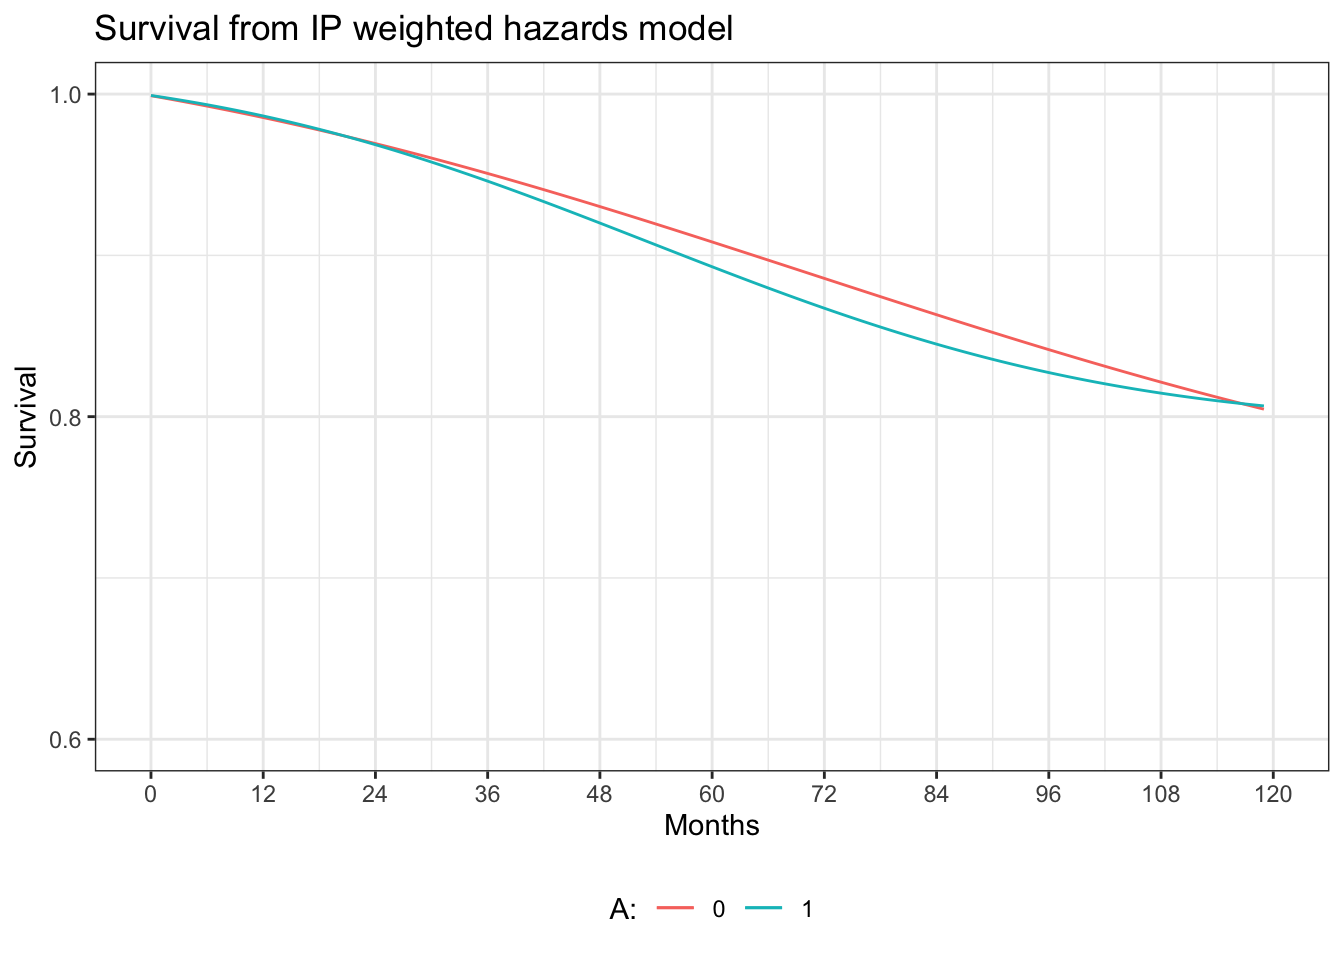
\includegraphics[width=0.85\linewidth]{17-causal-surv-r_files/figure-latex/unnamed-chunk-4-1} \end{center}

\hypertarget{program-17.4}{%
\section{Program 17.4}\label{program-17.4}}

\begin{itemize}
\tightlist
\item
  Estimating of survival curves via g-formula
\item
  Data from NHEFS
\end{itemize}

\begin{Shaded}
\begin{Highlighting}[]
\CommentTok{\# fit of hazards model with covariates}
\NormalTok{gf.model }\OtherTok{\textless{}{-}} \FunctionTok{glm}\NormalTok{(event}\SpecialCharTok{==}\DecValTok{0} \SpecialCharTok{\textasciitilde{}}\NormalTok{ qsmk }\SpecialCharTok{+} \FunctionTok{I}\NormalTok{(qsmk}\SpecialCharTok{*}\NormalTok{time) }\SpecialCharTok{+} \FunctionTok{I}\NormalTok{(qsmk}\SpecialCharTok{*}\NormalTok{timesq)}
                \SpecialCharTok{+}\NormalTok{ time }\SpecialCharTok{+}\NormalTok{ timesq }\SpecialCharTok{+}\NormalTok{ sex }\SpecialCharTok{+}\NormalTok{ race }\SpecialCharTok{+}\NormalTok{ age }\SpecialCharTok{+} \FunctionTok{I}\NormalTok{(age}\SpecialCharTok{*}\NormalTok{age)}
                \SpecialCharTok{+} \FunctionTok{as.factor}\NormalTok{(education) }\SpecialCharTok{+}\NormalTok{ smokeintensity }
                \SpecialCharTok{+} \FunctionTok{I}\NormalTok{(smokeintensity}\SpecialCharTok{*}\NormalTok{smokeintensity) }\SpecialCharTok{+}\NormalTok{ smkintensity82\_71 }
                \SpecialCharTok{+}\NormalTok{ smokeyrs }\SpecialCharTok{+} \FunctionTok{I}\NormalTok{(smokeyrs}\SpecialCharTok{*}\NormalTok{smokeyrs) }\SpecialCharTok{+} \FunctionTok{as.factor}\NormalTok{(exercise) }
                \SpecialCharTok{+} \FunctionTok{as.factor}\NormalTok{(active) }\SpecialCharTok{+}\NormalTok{ wt71 }\SpecialCharTok{+} \FunctionTok{I}\NormalTok{(wt71}\SpecialCharTok{*}\NormalTok{wt71), }
                \AttributeTok{data=}\NormalTok{nhefs.surv, }\AttributeTok{family=}\FunctionTok{binomial}\NormalTok{())}
\FunctionTok{summary}\NormalTok{(gf.model)}
\end{Highlighting}
\end{Shaded}

\begin{verbatim}
## 
## Call:
## glm(formula = event == 0 ~ qsmk + I(qsmk * time) + I(qsmk * timesq) + 
##     time + timesq + sex + race + age + I(age * age) + as.factor(education) + 
##     smokeintensity + I(smokeintensity * smokeintensity) + smkintensity82_71 + 
##     smokeyrs + I(smokeyrs * smokeyrs) + as.factor(exercise) + 
##     as.factor(active) + wt71 + I(wt71 * wt71), family = binomial(), 
##     data = nhefs.surv)
## 
## Deviance Residuals: 
##     Min       1Q   Median       3Q      Max  
## -4.3160   0.0244   0.0395   0.0640   0.3303  
## 
## Coefficients:
##                                      Estimate Std. Error z value Pr(>|z|)    
## (Intercept)                         9.272e+00  1.379e+00   6.724 1.76e-11 ***
## qsmk                                5.959e-02  4.154e-01   0.143 0.885924    
## I(qsmk * time)                     -1.485e-02  1.506e-02  -0.987 0.323824    
## I(qsmk * timesq)                    1.702e-04  1.245e-04   1.367 0.171643    
## time                               -2.270e-02  8.437e-03  -2.690 0.007142 ** 
## timesq                              1.174e-04  6.709e-05   1.751 0.080020 .  
## sex                                 4.368e-01  1.409e-01   3.101 0.001930 ** 
## race                               -5.240e-02  1.734e-01  -0.302 0.762572    
## age                                -8.750e-02  5.907e-02  -1.481 0.138536    
## I(age * age)                        8.128e-05  5.470e-04   0.149 0.881865    
## as.factor(education)2               1.401e-01  1.566e-01   0.895 0.370980    
## as.factor(education)3               4.335e-01  1.526e-01   2.841 0.004502 ** 
## as.factor(education)4               2.350e-01  2.790e-01   0.842 0.399750    
## as.factor(education)5               3.750e-01  2.386e-01   1.571 0.116115    
## smokeintensity                     -1.626e-03  1.430e-02  -0.114 0.909431    
## I(smokeintensity * smokeintensity) -7.182e-05  2.390e-04  -0.301 0.763741    
## smkintensity82_71                  -1.686e-03  6.501e-03  -0.259 0.795399    
## smokeyrs                           -1.677e-02  3.065e-02  -0.547 0.584153    
## I(smokeyrs * smokeyrs)             -5.280e-05  4.244e-04  -0.124 0.900997    
## as.factor(exercise)1                1.469e-01  1.792e-01   0.820 0.412300    
## as.factor(exercise)2               -1.504e-01  1.762e-01  -0.854 0.393177    
## as.factor(active)1                 -1.601e-01  1.300e-01  -1.232 0.218048    
## as.factor(active)2                 -2.294e-01  1.877e-01  -1.222 0.221766    
## wt71                                6.222e-02  1.902e-02   3.271 0.001073 ** 
## I(wt71 * wt71)                     -4.046e-04  1.129e-04  -3.584 0.000338 ***
## ---
## Signif. codes:  0 '***' 0.001 '**' 0.01 '*' 0.05 '.' 0.1 ' ' 1
## 
## (Dispersion parameter for binomial family taken to be 1)
## 
##     Null deviance: 4655.3  on 176763  degrees of freedom
## Residual deviance: 4185.7  on 176739  degrees of freedom
## AIC: 4235.7
## 
## Number of Fisher Scoring iterations: 10
\end{verbatim}

\begin{Shaded}
\begin{Highlighting}[]
\CommentTok{\# creation of dataset with all time points for }
\CommentTok{\# each individual under each treatment level}
\NormalTok{gf.qsmk0 }\OtherTok{\textless{}{-}} \FunctionTok{expandRows}\NormalTok{(nhefs, }\AttributeTok{count=}\DecValTok{120}\NormalTok{, }\AttributeTok{count.is.col=}\NormalTok{F) }
\NormalTok{gf.qsmk0}\SpecialCharTok{$}\NormalTok{time }\OtherTok{\textless{}{-}} \FunctionTok{rep}\NormalTok{(}\FunctionTok{seq}\NormalTok{(}\DecValTok{0}\NormalTok{, }\DecValTok{119}\NormalTok{), }\FunctionTok{nrow}\NormalTok{(nhefs))}
\NormalTok{gf.qsmk0}\SpecialCharTok{$}\NormalTok{timesq }\OtherTok{\textless{}{-}}\NormalTok{ gf.qsmk0}\SpecialCharTok{$}\NormalTok{time}\SpecialCharTok{\^{}}\DecValTok{2}
\NormalTok{gf.qsmk0}\SpecialCharTok{$}\NormalTok{qsmk }\OtherTok{\textless{}{-}} \DecValTok{0}

\NormalTok{gf.qsmk1 }\OtherTok{\textless{}{-}}\NormalTok{ gf.qsmk0}
\NormalTok{gf.qsmk1}\SpecialCharTok{$}\NormalTok{qsmk }\OtherTok{\textless{}{-}} \DecValTok{1}

\NormalTok{gf.qsmk0}\SpecialCharTok{$}\NormalTok{p.noevent0 }\OtherTok{\textless{}{-}} \FunctionTok{predict}\NormalTok{(gf.model, gf.qsmk0, }\AttributeTok{type=}\StringTok{"response"}\NormalTok{)}
\NormalTok{gf.qsmk1}\SpecialCharTok{$}\NormalTok{p.noevent1 }\OtherTok{\textless{}{-}} \FunctionTok{predict}\NormalTok{(gf.model, gf.qsmk1, }\AttributeTok{type=}\StringTok{"response"}\NormalTok{)}

\CommentTok{\#install.packages("dplyr")}
\FunctionTok{library}\NormalTok{(}\StringTok{"dplyr"}\NormalTok{)}
\end{Highlighting}
\end{Shaded}

\begin{verbatim}
## 
## Attaching package: 'dplyr'
\end{verbatim}

\begin{verbatim}
## The following objects are masked from 'package:stats':
## 
##     filter, lag
\end{verbatim}

\begin{verbatim}
## The following objects are masked from 'package:base':
## 
##     intersect, setdiff, setequal, union
\end{verbatim}

\begin{Shaded}
\begin{Highlighting}[]
\NormalTok{gf.qsmk0.surv }\OtherTok{\textless{}{-}}\NormalTok{ gf.qsmk0 }\SpecialCharTok{\%\textgreater{}\%} \FunctionTok{group\_by}\NormalTok{(seqn) }\SpecialCharTok{\%\textgreater{}\%} \FunctionTok{mutate}\NormalTok{(}\AttributeTok{surv0 =} \FunctionTok{cumprod}\NormalTok{(p.noevent0))}
\NormalTok{gf.qsmk1.surv }\OtherTok{\textless{}{-}}\NormalTok{ gf.qsmk1 }\SpecialCharTok{\%\textgreater{}\%} \FunctionTok{group\_by}\NormalTok{(seqn) }\SpecialCharTok{\%\textgreater{}\%} \FunctionTok{mutate}\NormalTok{(}\AttributeTok{surv1 =} \FunctionTok{cumprod}\NormalTok{(p.noevent1))}

\NormalTok{gf.surv0 }\OtherTok{\textless{}{-}} \FunctionTok{aggregate}\NormalTok{(gf.qsmk0.surv, }\AttributeTok{by=}\FunctionTok{list}\NormalTok{(gf.qsmk0.surv}\SpecialCharTok{$}\NormalTok{time), }\AttributeTok{FUN=}\NormalTok{mean)[}\FunctionTok{c}\NormalTok{(}\StringTok{"qsmk"}\NormalTok{, }\StringTok{"time"}\NormalTok{, }\StringTok{"surv0"}\NormalTok{)]}
\NormalTok{gf.surv1 }\OtherTok{\textless{}{-}} \FunctionTok{aggregate}\NormalTok{(gf.qsmk1.surv, }\AttributeTok{by=}\FunctionTok{list}\NormalTok{(gf.qsmk1.surv}\SpecialCharTok{$}\NormalTok{time), }\AttributeTok{FUN=}\NormalTok{mean)[}\FunctionTok{c}\NormalTok{(}\StringTok{"qsmk"}\NormalTok{, }\StringTok{"time"}\NormalTok{, }\StringTok{"surv1"}\NormalTok{)]}

\NormalTok{gf.graph }\OtherTok{\textless{}{-}} \FunctionTok{merge}\NormalTok{(gf.surv0, gf.surv1, }\AttributeTok{by=}\FunctionTok{c}\NormalTok{(}\StringTok{"time"}\NormalTok{))}
\NormalTok{gf.graph}\SpecialCharTok{$}\NormalTok{survdiff }\OtherTok{\textless{}{-}}\NormalTok{ gf.graph}\SpecialCharTok{$}\NormalTok{surv1}\SpecialCharTok{{-}}\NormalTok{gf.graph}\SpecialCharTok{$}\NormalTok{surv0}

\CommentTok{\# plot}
\FunctionTok{ggplot}\NormalTok{(gf.graph, }\FunctionTok{aes}\NormalTok{(}\AttributeTok{x=}\NormalTok{time, }\AttributeTok{y=}\NormalTok{surv)) }\SpecialCharTok{+} 
  \FunctionTok{geom\_line}\NormalTok{(}\FunctionTok{aes}\NormalTok{(}\AttributeTok{y =}\NormalTok{ surv0, }\AttributeTok{colour =} \StringTok{"0"}\NormalTok{)) }\SpecialCharTok{+} 
  \FunctionTok{geom\_line}\NormalTok{(}\FunctionTok{aes}\NormalTok{(}\AttributeTok{y =}\NormalTok{ surv1, }\AttributeTok{colour =} \StringTok{"1"}\NormalTok{)) }\SpecialCharTok{+} 
  \FunctionTok{xlab}\NormalTok{(}\StringTok{"Months"}\NormalTok{) }\SpecialCharTok{+} 
  \FunctionTok{scale\_x\_continuous}\NormalTok{(}\AttributeTok{limits =} \FunctionTok{c}\NormalTok{(}\DecValTok{0}\NormalTok{, }\DecValTok{120}\NormalTok{), }\AttributeTok{breaks=}\FunctionTok{seq}\NormalTok{(}\DecValTok{0}\NormalTok{,}\DecValTok{120}\NormalTok{,}\DecValTok{12}\NormalTok{)) }\SpecialCharTok{+}
  \FunctionTok{scale\_y\_continuous}\NormalTok{(}\AttributeTok{limits=}\FunctionTok{c}\NormalTok{(}\FloatTok{0.6}\NormalTok{, }\DecValTok{1}\NormalTok{), }\AttributeTok{breaks=}\FunctionTok{seq}\NormalTok{(}\FloatTok{0.6}\NormalTok{, }\DecValTok{1}\NormalTok{, }\FloatTok{0.2}\NormalTok{)) }\SpecialCharTok{+}
  \FunctionTok{ylab}\NormalTok{(}\StringTok{"Survival"}\NormalTok{) }\SpecialCharTok{+} 
  \FunctionTok{ggtitle}\NormalTok{(}\StringTok{"Survival from g{-}formula"}\NormalTok{) }\SpecialCharTok{+} 
  \FunctionTok{labs}\NormalTok{(}\AttributeTok{colour=}\StringTok{"A:"}\NormalTok{) }\SpecialCharTok{+}
  \FunctionTok{theme\_bw}\NormalTok{() }\SpecialCharTok{+} 
  \FunctionTok{theme}\NormalTok{(}\AttributeTok{legend.position=}\StringTok{"bottom"}\NormalTok{)}
\end{Highlighting}
\end{Shaded}

\begin{center}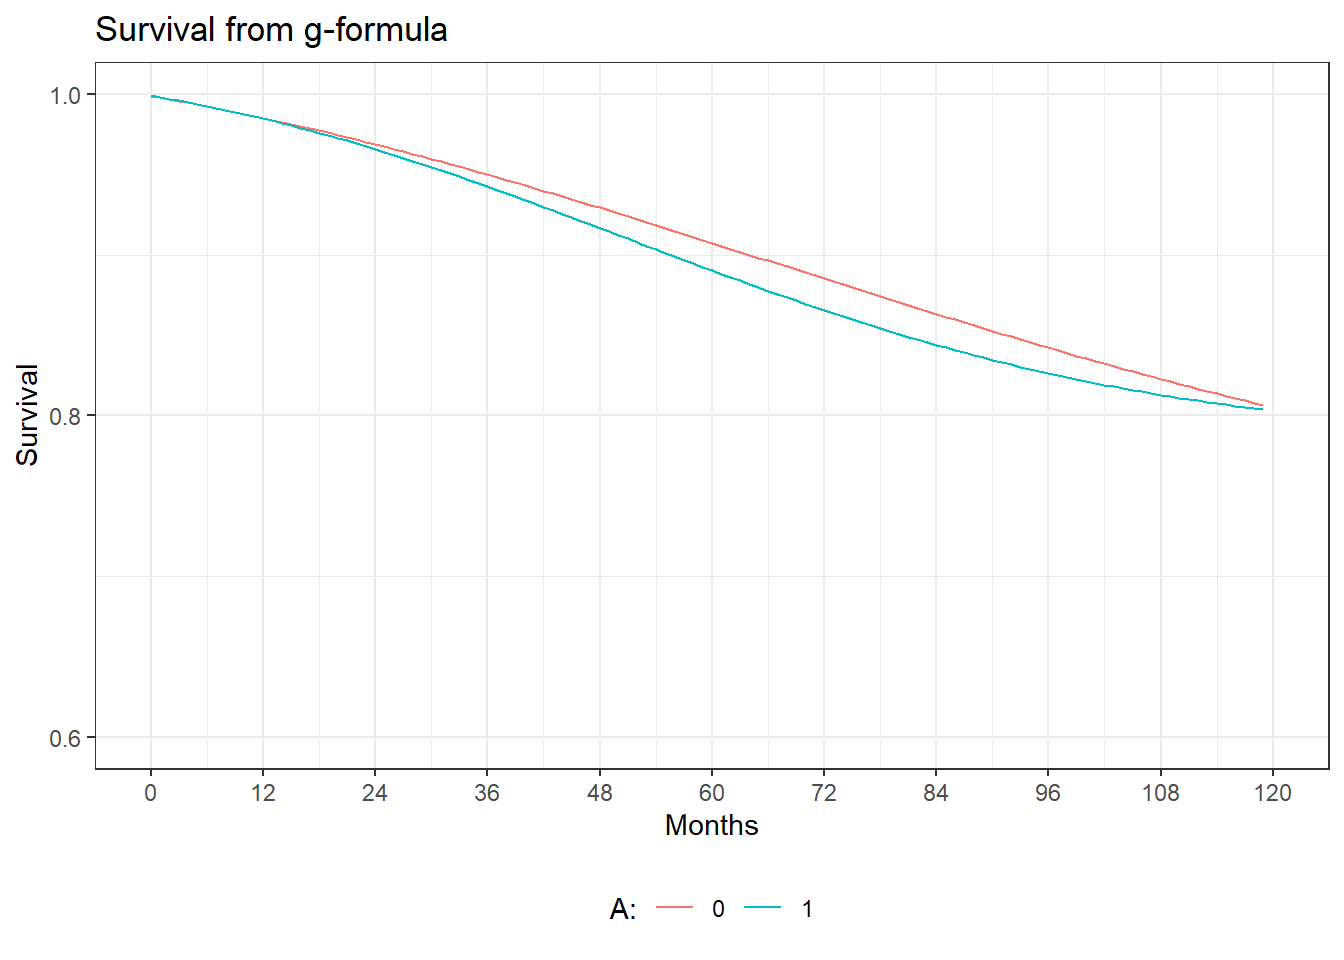
\includegraphics[width=0.85\linewidth]{17-causal-surv-r_files/figure-latex/unnamed-chunk-5-1} \end{center}

\hypertarget{program-17.5}{%
\section{Program 17.5}\label{program-17.5}}

\begin{itemize}
\tightlist
\item
  Estimating of median survival time ratio via a structural nested AFT model
\item
  Data from NHEFS
\end{itemize}

\begin{Shaded}
\begin{Highlighting}[]
\CommentTok{\# some preprocessing of the data}
\NormalTok{nhefs }\OtherTok{\textless{}{-}} \FunctionTok{read\_excel}\NormalTok{(}\FunctionTok{here}\NormalTok{(}\StringTok{"data"}\NormalTok{, }\StringTok{"NHEFS.xls"}\NormalTok{))}
\NormalTok{nhefs}\SpecialCharTok{$}\NormalTok{survtime }\OtherTok{\textless{}{-}} \FunctionTok{ifelse}\NormalTok{(nhefs}\SpecialCharTok{$}\NormalTok{death}\SpecialCharTok{==}\DecValTok{0}\NormalTok{, }\ConstantTok{NA}\NormalTok{, (nhefs}\SpecialCharTok{$}\NormalTok{yrdth}\DecValTok{{-}83}\NormalTok{)}\SpecialCharTok{*}\DecValTok{12}\SpecialCharTok{+}\NormalTok{nhefs}\SpecialCharTok{$}\NormalTok{modth) }\CommentTok{\# * yrdth ranges from 83 to 92}

\CommentTok{\# model to estimate E[A|L]}
\NormalTok{modelA }\OtherTok{\textless{}{-}} \FunctionTok{glm}\NormalTok{(qsmk }\SpecialCharTok{\textasciitilde{}}\NormalTok{ sex }\SpecialCharTok{+}\NormalTok{ race }\SpecialCharTok{+}\NormalTok{ age }\SpecialCharTok{+} \FunctionTok{I}\NormalTok{(age}\SpecialCharTok{*}\NormalTok{age)}
              \SpecialCharTok{+} \FunctionTok{as.factor}\NormalTok{(education) }\SpecialCharTok{+}\NormalTok{ smokeintensity}
              \SpecialCharTok{+} \FunctionTok{I}\NormalTok{(smokeintensity}\SpecialCharTok{*}\NormalTok{smokeintensity) }\SpecialCharTok{+}\NormalTok{ smokeyrs}
              \SpecialCharTok{+} \FunctionTok{I}\NormalTok{(smokeyrs}\SpecialCharTok{*}\NormalTok{smokeyrs) }\SpecialCharTok{+} \FunctionTok{as.factor}\NormalTok{(exercise)}
              \SpecialCharTok{+} \FunctionTok{as.factor}\NormalTok{(active) }\SpecialCharTok{+}\NormalTok{ wt71 }\SpecialCharTok{+} \FunctionTok{I}\NormalTok{(wt71}\SpecialCharTok{*}\NormalTok{wt71),}
              \AttributeTok{data=}\NormalTok{nhefs, }\AttributeTok{family=}\FunctionTok{binomial}\NormalTok{())}

\NormalTok{nhefs}\SpecialCharTok{$}\NormalTok{p.qsmk }\OtherTok{\textless{}{-}} \FunctionTok{predict}\NormalTok{(modelA, nhefs, }\AttributeTok{type=}\StringTok{"response"}\NormalTok{) }
\NormalTok{d }\OtherTok{\textless{}{-}}\NormalTok{ nhefs[}\SpecialCharTok{!}\FunctionTok{is.na}\NormalTok{(nhefs}\SpecialCharTok{$}\NormalTok{survtime),] }\CommentTok{\# select only those with observed death time}
\NormalTok{n }\OtherTok{\textless{}{-}} \FunctionTok{nrow}\NormalTok{(d)}

\CommentTok{\# define the estimating function that needs to be minimized}
\NormalTok{sumeef }\OtherTok{\textless{}{-}} \ControlFlowTok{function}\NormalTok{(psi)\{}
  
  \CommentTok{\# creation of delta indicator}
  \ControlFlowTok{if}\NormalTok{ (psi}\SpecialCharTok{\textgreater{}=}\DecValTok{0}\NormalTok{)\{}
\NormalTok{    delta }\OtherTok{\textless{}{-}} \FunctionTok{ifelse}\NormalTok{(d}\SpecialCharTok{$}\NormalTok{qsmk}\SpecialCharTok{==}\DecValTok{0} \SpecialCharTok{|} 
\NormalTok{                      (d}\SpecialCharTok{$}\NormalTok{qsmk}\SpecialCharTok{==}\DecValTok{1} \SpecialCharTok{\&}\NormalTok{ psi }\SpecialCharTok{\textless{}=} \FunctionTok{log}\NormalTok{(}\DecValTok{120}\SpecialCharTok{/}\NormalTok{d}\SpecialCharTok{$}\NormalTok{survtime)), }
                    \DecValTok{1}\NormalTok{, }\DecValTok{0}\NormalTok{)}
\NormalTok{  \} }\ControlFlowTok{else} \ControlFlowTok{if}\NormalTok{ (psi }\SpecialCharTok{\textless{}} \DecValTok{0}\NormalTok{) \{}
\NormalTok{    delta }\OtherTok{\textless{}{-}} \FunctionTok{ifelse}\NormalTok{(d}\SpecialCharTok{$}\NormalTok{qsmk}\SpecialCharTok{==}\DecValTok{1} \SpecialCharTok{|} 
\NormalTok{                      (d}\SpecialCharTok{$}\NormalTok{qsmk}\SpecialCharTok{==}\DecValTok{0} \SpecialCharTok{\&}\NormalTok{ psi }\SpecialCharTok{\textgreater{}} \FunctionTok{log}\NormalTok{(d}\SpecialCharTok{$}\NormalTok{survtime}\SpecialCharTok{/}\DecValTok{120}\NormalTok{)), }\DecValTok{1}\NormalTok{, }\DecValTok{0}\NormalTok{)}
\NormalTok{  \}}
  
\NormalTok{  smat }\OtherTok{\textless{}{-}}\NormalTok{ delta}\SpecialCharTok{*}\NormalTok{(d}\SpecialCharTok{$}\NormalTok{qsmk}\SpecialCharTok{{-}}\NormalTok{d}\SpecialCharTok{$}\NormalTok{p.qsmk)}
\NormalTok{  sval }\OtherTok{\textless{}{-}} \FunctionTok{sum}\NormalTok{(smat, }\AttributeTok{na.rm=}\NormalTok{T)}
\NormalTok{  save }\OtherTok{\textless{}{-}}\NormalTok{ sval}\SpecialCharTok{/}\NormalTok{n}
\NormalTok{  smat }\OtherTok{\textless{}{-}}\NormalTok{ smat }\SpecialCharTok{{-}} \FunctionTok{rep}\NormalTok{(save, n)}
  
  \CommentTok{\# covariance}
\NormalTok{  sigma }\OtherTok{\textless{}{-}} \FunctionTok{t}\NormalTok{(smat) }\SpecialCharTok{\%*\%}\NormalTok{ smat}
  \ControlFlowTok{if}\NormalTok{ (sigma }\SpecialCharTok{==} \DecValTok{0}\NormalTok{)\{}
\NormalTok{    sigma }\OtherTok{\textless{}{-}} \FloatTok{1e{-}16}
\NormalTok{  \}}
\NormalTok{  estimeq }\OtherTok{\textless{}{-}}\NormalTok{ sval}\SpecialCharTok{*}\FunctionTok{solve}\NormalTok{(sigma)}\SpecialCharTok{*}\FunctionTok{t}\NormalTok{(sval)}
  \FunctionTok{return}\NormalTok{(estimeq)}
\NormalTok{\}}

\NormalTok{res }\OtherTok{\textless{}{-}} \FunctionTok{optimize}\NormalTok{(sumeef, }\AttributeTok{interval =} \FunctionTok{c}\NormalTok{(}\SpecialCharTok{{-}}\FloatTok{0.2}\NormalTok{,}\FloatTok{0.2}\NormalTok{))}
\NormalTok{psi1 }\OtherTok{\textless{}{-}}\NormalTok{ res}\SpecialCharTok{$}\NormalTok{minimum}
\NormalTok{objfunc }\OtherTok{\textless{}{-}} \FunctionTok{as.numeric}\NormalTok{(res}\SpecialCharTok{$}\NormalTok{objective)}


\CommentTok{\# Use simple bisection method to find estimates of lower and upper 95\% confidence bounds}
\NormalTok{increm }\OtherTok{\textless{}{-}} \FloatTok{0.1}
\NormalTok{for\_conf }\OtherTok{\textless{}{-}} \ControlFlowTok{function}\NormalTok{(x)\{}
  \FunctionTok{return}\NormalTok{(}\FunctionTok{sumeef}\NormalTok{(x) }\SpecialCharTok{{-}} \FloatTok{3.84}\NormalTok{)}
\NormalTok{\}}

\ControlFlowTok{if}\NormalTok{ (objfunc }\SpecialCharTok{\textless{}} \FloatTok{3.84}\NormalTok{)\{}
  \CommentTok{\# Find estimate of where sumeef(x) \textgreater{} 3.84}
  
  \CommentTok{\# Lower bound of 95\% CI}
\NormalTok{  psilow }\OtherTok{\textless{}{-}}\NormalTok{ psi1}
\NormalTok{  testlow }\OtherTok{\textless{}{-}}\NormalTok{ objfunc}
\NormalTok{  countlow }\OtherTok{\textless{}{-}} \DecValTok{0}
  \ControlFlowTok{while}\NormalTok{ (testlow }\SpecialCharTok{\textless{}} \FloatTok{3.84} \SpecialCharTok{\&}\NormalTok{ countlow }\SpecialCharTok{\textless{}} \DecValTok{100}\NormalTok{)\{}
\NormalTok{    psilow }\OtherTok{\textless{}{-}}\NormalTok{ psilow }\SpecialCharTok{{-}}\NormalTok{ increm}
\NormalTok{    testlow }\OtherTok{\textless{}{-}} \FunctionTok{sumeef}\NormalTok{(psilow)}
\NormalTok{    countlow }\OtherTok{\textless{}{-}}\NormalTok{ countlow }\SpecialCharTok{+} \DecValTok{1}
\NormalTok{  \}}
  
  \CommentTok{\# Upper bound of 95\% CI}
\NormalTok{  psihigh }\OtherTok{\textless{}{-}}\NormalTok{ psi1}
\NormalTok{  testhigh }\OtherTok{\textless{}{-}}\NormalTok{ objfunc}
\NormalTok{  counthigh }\OtherTok{\textless{}{-}} \DecValTok{0}
  \ControlFlowTok{while}\NormalTok{ (testhigh }\SpecialCharTok{\textless{}} \FloatTok{3.84} \SpecialCharTok{\&}\NormalTok{ counthigh }\SpecialCharTok{\textless{}} \DecValTok{100}\NormalTok{)\{}
\NormalTok{    psihigh }\OtherTok{\textless{}{-}}\NormalTok{ psihigh }\SpecialCharTok{+}\NormalTok{ increm}
\NormalTok{    testhigh }\OtherTok{\textless{}{-}} \FunctionTok{sumeef}\NormalTok{(psihigh)}
\NormalTok{    counthigh }\OtherTok{\textless{}{-}}\NormalTok{ counthigh }\SpecialCharTok{+} \DecValTok{1}
\NormalTok{  \}}
  
  \CommentTok{\# Better estimate using bisection method}
  \ControlFlowTok{if}\NormalTok{ ((testhigh }\SpecialCharTok{\textgreater{}} \FloatTok{3.84}\NormalTok{) }\SpecialCharTok{\&}\NormalTok{ (testlow }\SpecialCharTok{\textgreater{}} \FloatTok{3.84}\NormalTok{))\{}
    
    \CommentTok{\# Bisection method}
\NormalTok{    left }\OtherTok{\textless{}{-}}\NormalTok{ psi1}
\NormalTok{    fleft }\OtherTok{\textless{}{-}}\NormalTok{ objfunc }\SpecialCharTok{{-}} \FloatTok{3.84}
\NormalTok{    right }\OtherTok{\textless{}{-}}\NormalTok{ psihigh}
\NormalTok{    fright }\OtherTok{\textless{}{-}}\NormalTok{ testhigh }\SpecialCharTok{{-}} \FloatTok{3.84}
\NormalTok{    middle }\OtherTok{\textless{}{-}}\NormalTok{ (left  }\SpecialCharTok{+}\NormalTok{ right) }\SpecialCharTok{/} \DecValTok{2}
\NormalTok{    fmiddle }\OtherTok{\textless{}{-}} \FunctionTok{for\_conf}\NormalTok{(middle)}
\NormalTok{    count }\OtherTok{\textless{}{-}} \DecValTok{0}
\NormalTok{    diff }\OtherTok{\textless{}{-}}\NormalTok{ right }\SpecialCharTok{{-}}\NormalTok{ left}
    
    \ControlFlowTok{while}\NormalTok{ (}\SpecialCharTok{!}\NormalTok{(}\FunctionTok{abs}\NormalTok{(fmiddle) }\SpecialCharTok{\textless{}} \FloatTok{0.0001} \SpecialCharTok{|}\NormalTok{ diff }\SpecialCharTok{\textless{}} \FloatTok{0.0001} \SpecialCharTok{|}\NormalTok{ count }\SpecialCharTok{\textgreater{}} \DecValTok{100}\NormalTok{))\{}
\NormalTok{      test }\OtherTok{\textless{}{-}}\NormalTok{ fmiddle }\SpecialCharTok{*}\NormalTok{ fleft}
      \ControlFlowTok{if}\NormalTok{ (test }\SpecialCharTok{\textless{}} \DecValTok{0}\NormalTok{)\{}
\NormalTok{        right }\OtherTok{\textless{}{-}}\NormalTok{ middle}
\NormalTok{        fright }\OtherTok{\textless{}{-}}\NormalTok{ fmiddle}
\NormalTok{      \} }\ControlFlowTok{else}\NormalTok{ \{}
\NormalTok{        left }\OtherTok{\textless{}{-}}\NormalTok{ middle}
\NormalTok{        fleft }\OtherTok{\textless{}{-}}\NormalTok{ fmiddle}
\NormalTok{      \}}
\NormalTok{      middle }\OtherTok{\textless{}{-}}\NormalTok{ (left }\SpecialCharTok{+}\NormalTok{ right) }\SpecialCharTok{/} \DecValTok{2}
\NormalTok{      fmiddle }\OtherTok{\textless{}{-}} \FunctionTok{for\_conf}\NormalTok{(middle)}
\NormalTok{      count }\OtherTok{\textless{}{-}}\NormalTok{ count }\SpecialCharTok{+} \DecValTok{1}
\NormalTok{      diff }\OtherTok{\textless{}{-}}\NormalTok{ right }\SpecialCharTok{{-}}\NormalTok{ left}
\NormalTok{    \}}
    
\NormalTok{    psi\_high }\OtherTok{\textless{}{-}}\NormalTok{ middle}
\NormalTok{    objfunc\_high }\OtherTok{\textless{}{-}}\NormalTok{ fmiddle }\SpecialCharTok{+} \FloatTok{3.84}
    
    \CommentTok{\# lower bound of 95\% CI}
\NormalTok{    left }\OtherTok{\textless{}{-}}\NormalTok{ psilow}
\NormalTok{    fleft }\OtherTok{\textless{}{-}}\NormalTok{ testlow }\SpecialCharTok{{-}} \FloatTok{3.84}
\NormalTok{    right }\OtherTok{\textless{}{-}}\NormalTok{ psi1}
\NormalTok{    fright }\OtherTok{\textless{}{-}}\NormalTok{ objfunc }\SpecialCharTok{{-}} \FloatTok{3.84}
\NormalTok{    middle }\OtherTok{\textless{}{-}}\NormalTok{ (left }\SpecialCharTok{+}\NormalTok{ right) }\SpecialCharTok{/} \DecValTok{2}
\NormalTok{    fmiddle }\OtherTok{\textless{}{-}} \FunctionTok{for\_conf}\NormalTok{(middle)}
\NormalTok{    count }\OtherTok{\textless{}{-}} \DecValTok{0}
\NormalTok{    diff }\OtherTok{\textless{}{-}}\NormalTok{ right }\SpecialCharTok{{-}}\NormalTok{ left}
    
    \ControlFlowTok{while}\NormalTok{(}\SpecialCharTok{!}\NormalTok{(}\FunctionTok{abs}\NormalTok{(fmiddle) }\SpecialCharTok{\textless{}} \FloatTok{0.0001} \SpecialCharTok{|}\NormalTok{ diff }\SpecialCharTok{\textless{}} \FloatTok{0.0001} \SpecialCharTok{|}\NormalTok{ count }\SpecialCharTok{\textgreater{}} \DecValTok{100}\NormalTok{))\{}
\NormalTok{      test }\OtherTok{\textless{}{-}}\NormalTok{ fmiddle }\SpecialCharTok{*}\NormalTok{ fleft}
      \ControlFlowTok{if}\NormalTok{ (test }\SpecialCharTok{\textless{}} \DecValTok{0}\NormalTok{)\{}
\NormalTok{        right }\OtherTok{\textless{}{-}}\NormalTok{ middle}
\NormalTok{        fright }\OtherTok{\textless{}{-}}\NormalTok{ fmiddle}
\NormalTok{      \} }\ControlFlowTok{else}\NormalTok{ \{}
\NormalTok{        left }\OtherTok{\textless{}{-}}\NormalTok{ middle}
\NormalTok{        fleft }\OtherTok{\textless{}{-}}\NormalTok{ fmiddle}
\NormalTok{      \}}
\NormalTok{      middle }\OtherTok{\textless{}{-}}\NormalTok{ (left }\SpecialCharTok{+}\NormalTok{ right) }\SpecialCharTok{/} \DecValTok{2}
\NormalTok{      fmiddle }\OtherTok{\textless{}{-}} \FunctionTok{for\_conf}\NormalTok{(middle)}
\NormalTok{      diff }\OtherTok{\textless{}{-}}\NormalTok{ right }\SpecialCharTok{{-}}\NormalTok{ left}
\NormalTok{      count }\OtherTok{\textless{}{-}}\NormalTok{ count }\SpecialCharTok{+} \DecValTok{1}
\NormalTok{    \}}
\NormalTok{    psi\_low }\OtherTok{\textless{}{-}}\NormalTok{ middle}
\NormalTok{    objfunc\_low }\OtherTok{\textless{}{-}}\NormalTok{ fmiddle }\SpecialCharTok{+} \FloatTok{3.84}
\NormalTok{    psi }\OtherTok{\textless{}{-}}\NormalTok{ psi1}
\NormalTok{  \}}
\NormalTok{\}}
\FunctionTok{c}\NormalTok{(psi, psi\_low, psi\_high)}
\end{Highlighting}
\end{Shaded}

\begin{verbatim}
## [1] -0.05041591 -0.22312099  0.33312901
\end{verbatim}

\hypertarget{session-information-r}{%
\chapter*{Session information: R}\label{session-information-r}}
\addcontentsline{toc}{chapter}{Session information: R}

For reproducibility.

\begin{Shaded}
\begin{Highlighting}[]
\CommentTok{\# install.packages("sessioninfo")}
\NormalTok{sessioninfo}\SpecialCharTok{::}\FunctionTok{session\_info}\NormalTok{()}
\end{Highlighting}
\end{Shaded}

\begin{verbatim}
## - Session info ---------------------------------------------------------------
##  setting  value
##  version  R version 4.2.1 (2022-06-23)
##  os       macOS Monterey 12.4
##  system   aarch64, darwin20
##  ui       X11
##  language (EN)
##  collate  en_GB.UTF-8
##  ctype    en_GB.UTF-8
##  tz       Europe/London
##  date     2022-07-05
##  pandoc   2.18 @ /Applications/RStudio.app/Contents/MacOS/quarto/bin/tools/ (via rmarkdown)
## 
## - Packages -------------------------------------------------------------------
##  package     * version date (UTC) lib source
##  bookdown      0.27    2022-06-14 [3] CRAN (R 4.2.0)
##  cli           3.3.0   2022-04-25 [3] CRAN (R 4.2.0)
##  digest        0.6.29  2021-12-01 [3] CRAN (R 4.2.0)
##  evaluate      0.15    2022-02-18 [3] CRAN (R 4.2.0)
##  fastmap       1.1.0   2021-01-25 [3] CRAN (R 4.2.0)
##  htmltools     0.5.2   2021-08-25 [3] CRAN (R 4.2.0)
##  knitr         1.39    2022-04-26 [3] CRAN (R 4.2.0)
##  magrittr      2.0.3   2022-03-30 [3] CRAN (R 4.2.0)
##  rlang         1.0.3   2022-06-27 [3] CRAN (R 4.2.1)
##  rmarkdown     2.14    2022-04-25 [3] CRAN (R 4.2.0)
##  rstudioapi    0.13    2020-11-12 [3] CRAN (R 4.2.0)
##  sessioninfo   1.2.2   2021-12-06 [3] CRAN (R 4.2.0)
##  stringi       1.7.6   2021-11-29 [3] CRAN (R 4.2.0)
##  stringr       1.4.0   2019-02-10 [3] CRAN (R 4.2.0)
##  xfun          0.31    2022-05-10 [3] CRAN (R 4.2.0)
##  yaml          2.3.5   2022-02-21 [3] CRAN (R 4.2.0)
## 
##  [1] /Users/tom/Library/R/arm64/4.2/library
##  [2] /Library/Frameworks/R.framework/Versions/4.2-arm64/Resources/site-library
##  [3] /Library/Frameworks/R.framework/Versions/4.2-arm64/Resources/library
## 
## ------------------------------------------------------------------------------
\end{verbatim}

\hypertarget{part-stata-code}{%
\part*{Stata code}\label{part-stata-code}}
\addcontentsline{toc}{part}{Stata code}

\hypertarget{why-model-stata}{%
\chapter*{11. Why model: Stata}\label{why-model-stata}}
\addcontentsline{toc}{chapter}{11. Why model: Stata}

\begin{Shaded}
\begin{Highlighting}[]
\FunctionTok{library}\NormalTok{(Statamarkdown)}
\end{Highlighting}
\end{Shaded}

\begin{Shaded}
\begin{Highlighting}[]
\KeywordTok{do}\NormalTok{ dependency}
\end{Highlighting}
\end{Shaded}

\begin{verbatim}
checking extremes consistency and verifying not already installed...
all files already exist and are up to date.

checking tomata consistency and verifying not already installed...
all files already exist and are up to date.

end of do-file
\end{verbatim}

\begin{verbatim}
/***************************************************************
Stata code for Causal Inference: What If by Miguel Hernan & Jamie Robins
Date: 10/10/2019
Author: Eleanor Murray 
For errors contact: ejmurray@bu.edu
***************************************************************/
\end{verbatim}

\hypertarget{program-11.1-1}{%
\section{Program 11.1}\label{program-11.1-1}}

\begin{itemize}
\tightlist
\item
  Figures 11.1, 11.2, and 11.3
\item
  Sample averages by treatment level
\end{itemize}

\begin{Shaded}
\begin{Highlighting}[]
\KeywordTok{clear}

\NormalTok{**Figure 11.1**}
\NormalTok{*create the dataset*}
\NormalTok{input A Y}
\NormalTok{1 200}
\NormalTok{1 150}
\NormalTok{1 220}
\NormalTok{1 110}
\NormalTok{1 50}
\NormalTok{1 180}
\NormalTok{1 90}
\NormalTok{1 170}
\NormalTok{0 170}
\NormalTok{0 30}
\NormalTok{0 70}
\NormalTok{0 110}
\NormalTok{0 80}
\NormalTok{0 50}
\NormalTok{0 10}
\NormalTok{0 20}
\KeywordTok{end}

\NormalTok{*Save the }\KeywordTok{data}\NormalTok{*}
\KeywordTok{qui} \KeywordTok{save}\NormalTok{ ./}\KeywordTok{data}\NormalTok{/fig1, }\KeywordTok{replace}

\NormalTok{*Build the scatterplot*}
\KeywordTok{scatter}\NormalTok{ Y A, ylab(0(50)250) xlab(0 1) }\BaseNTok{xscale}\NormalTok{(}\KeywordTok{range}\NormalTok{({-}0.5 1.5))}
\KeywordTok{qui} \KeywordTok{gr} \KeywordTok{export}\NormalTok{ figs/stata{-}fig{-}11{-}1.png, }\KeywordTok{replace}

\NormalTok{*Output the }\KeywordTok{mean} \KeywordTok{values} \KeywordTok{for}\NormalTok{ Y }\KeywordTok{in}\NormalTok{ each }\DecValTok{level} \KeywordTok{of}\NormalTok{ A*}
\KeywordTok{bysort}\NormalTok{ A: }\KeywordTok{sum}\NormalTok{ Y}
\end{Highlighting}
\end{Shaded}

\begin{verbatim}
             A          Y
  1. 1 200
  2. 1 150
  3. 1 220
  4. 1 110
  5. 1 50
  6. 1 180
  7. 1 90
  8. 1 170
  9. 0 170
 10. 0 30
 11. 0 70
 12. 0 110
 13. 0 80
 14. 0 50
 15. 0 10
 16. 0 20
 17. end





--------------------------------------------------------------------------------
-> A = 0

    Variable |        Obs        Mean    Std. dev.       Min        Max
-------------+---------------------------------------------------------
           Y |          8        67.5    53.11712         10        170

--------------------------------------------------------------------------------
-> A = 1

    Variable |        Obs        Mean    Std. dev.       Min        Max
-------------+---------------------------------------------------------
           Y |          8      146.25     58.2942         50        220
\end{verbatim}

\begin{center}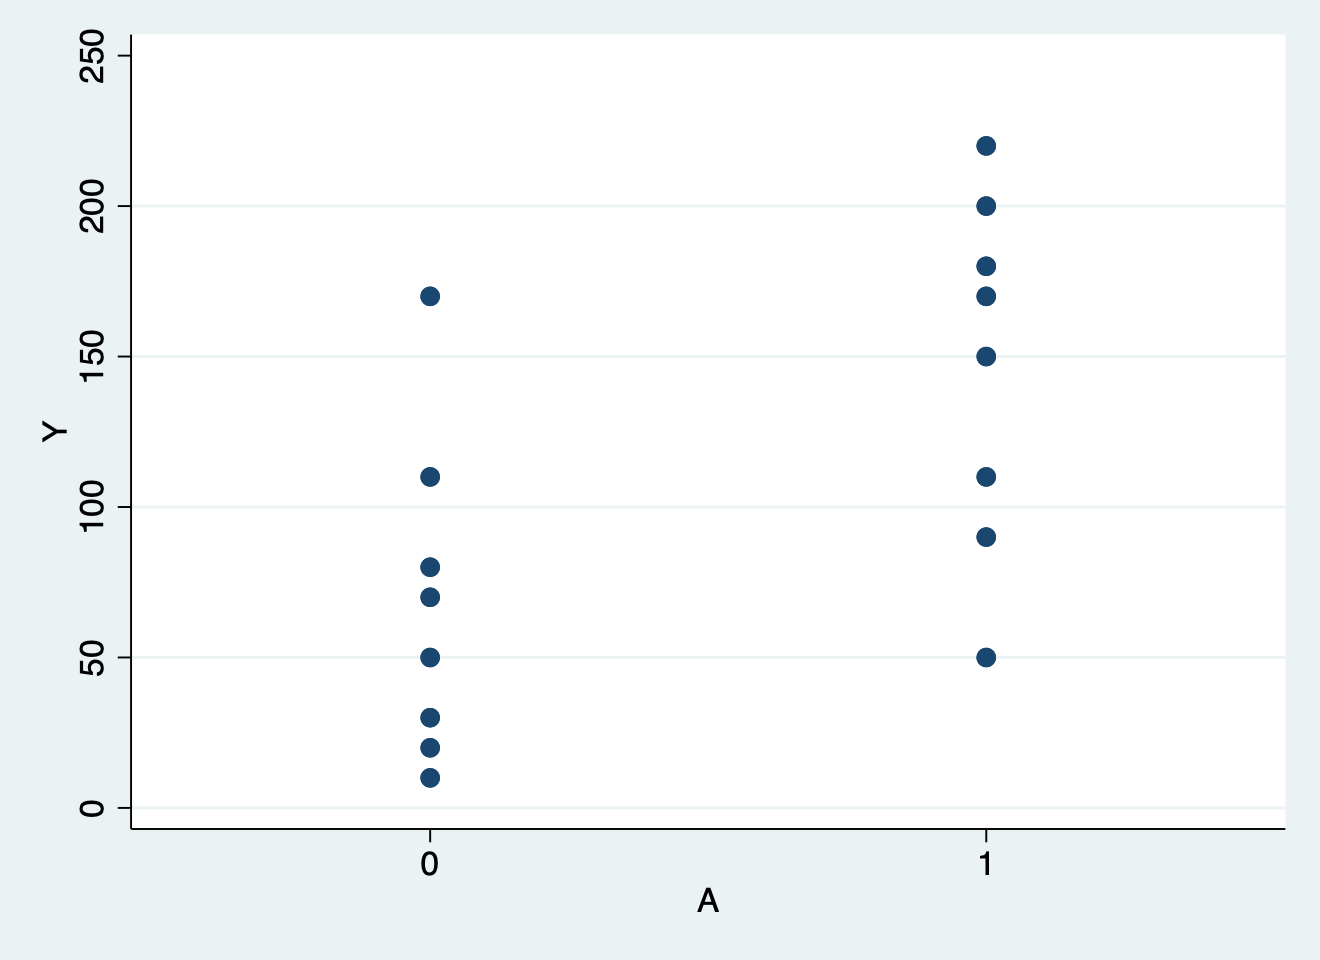
\includegraphics[width=0.85\linewidth]{figs/stata-fig-11-1} \end{center}

\begin{Shaded}
\begin{Highlighting}[]
\NormalTok{*Clear the workspace to }\KeywordTok{be}\NormalTok{ able to }\KeywordTok{use}\NormalTok{ a }\KeywordTok{new}\NormalTok{ dataset*}
\KeywordTok{clear}

\NormalTok{**Figure 11.2**}
\NormalTok{input A Y}
\NormalTok{1 110}
\NormalTok{1 80}
\NormalTok{1 50}
\NormalTok{1 40}
\NormalTok{2 170}
\NormalTok{2 30}
\NormalTok{2 70}
\NormalTok{2 50}
\NormalTok{3 110}
\NormalTok{3 50}
\NormalTok{3 180}
\NormalTok{3 130}
\NormalTok{4 200}
\NormalTok{4 150}
\NormalTok{4 220}
\NormalTok{4 210}
\KeywordTok{end}

\KeywordTok{qui} \KeywordTok{save}\NormalTok{ ./}\KeywordTok{data}\NormalTok{/fig2, }\KeywordTok{replace}

\KeywordTok{scatter}\NormalTok{ Y A, ylab(0(50)250) xlab(0(1)4) }\BaseNTok{xscale}\NormalTok{(}\KeywordTok{range}\NormalTok{(0 4.5))}
\KeywordTok{qui} \KeywordTok{gr} \KeywordTok{export}\NormalTok{ figs/stata{-}fig{-}11{-}2.png, }\KeywordTok{replace}

\KeywordTok{bysort}\NormalTok{ A: }\KeywordTok{sum}\NormalTok{ Y}
\end{Highlighting}
\end{Shaded}

\begin{verbatim}
             A          Y
  1. 1 110
  2. 1 80
  3. 1 50
  4. 1 40
  5. 2 170
  6. 2 30
  7. 2 70
  8. 2 50
  9. 3 110
 10. 3 50
 11. 3 180
 12. 3 130
 13. 4 200
 14. 4 150
 15. 4 220
 16. 4 210
 17. end





--------------------------------------------------------------------------------
-> A = 1

    Variable |        Obs        Mean    Std. dev.       Min        Max
-------------+---------------------------------------------------------
           Y |          4          70    31.62278         40        110

--------------------------------------------------------------------------------
-> A = 2

    Variable |        Obs        Mean    Std. dev.       Min        Max
-------------+---------------------------------------------------------
           Y |          4          80    62.18253         30        170

--------------------------------------------------------------------------------
-> A = 3

    Variable |        Obs        Mean    Std. dev.       Min        Max
-------------+---------------------------------------------------------
           Y |          4       117.5    53.77422         50        180

--------------------------------------------------------------------------------
-> A = 4

    Variable |        Obs        Mean    Std. dev.       Min        Max
-------------+---------------------------------------------------------
           Y |          4         195    31.09126        150        220
\end{verbatim}

\begin{center}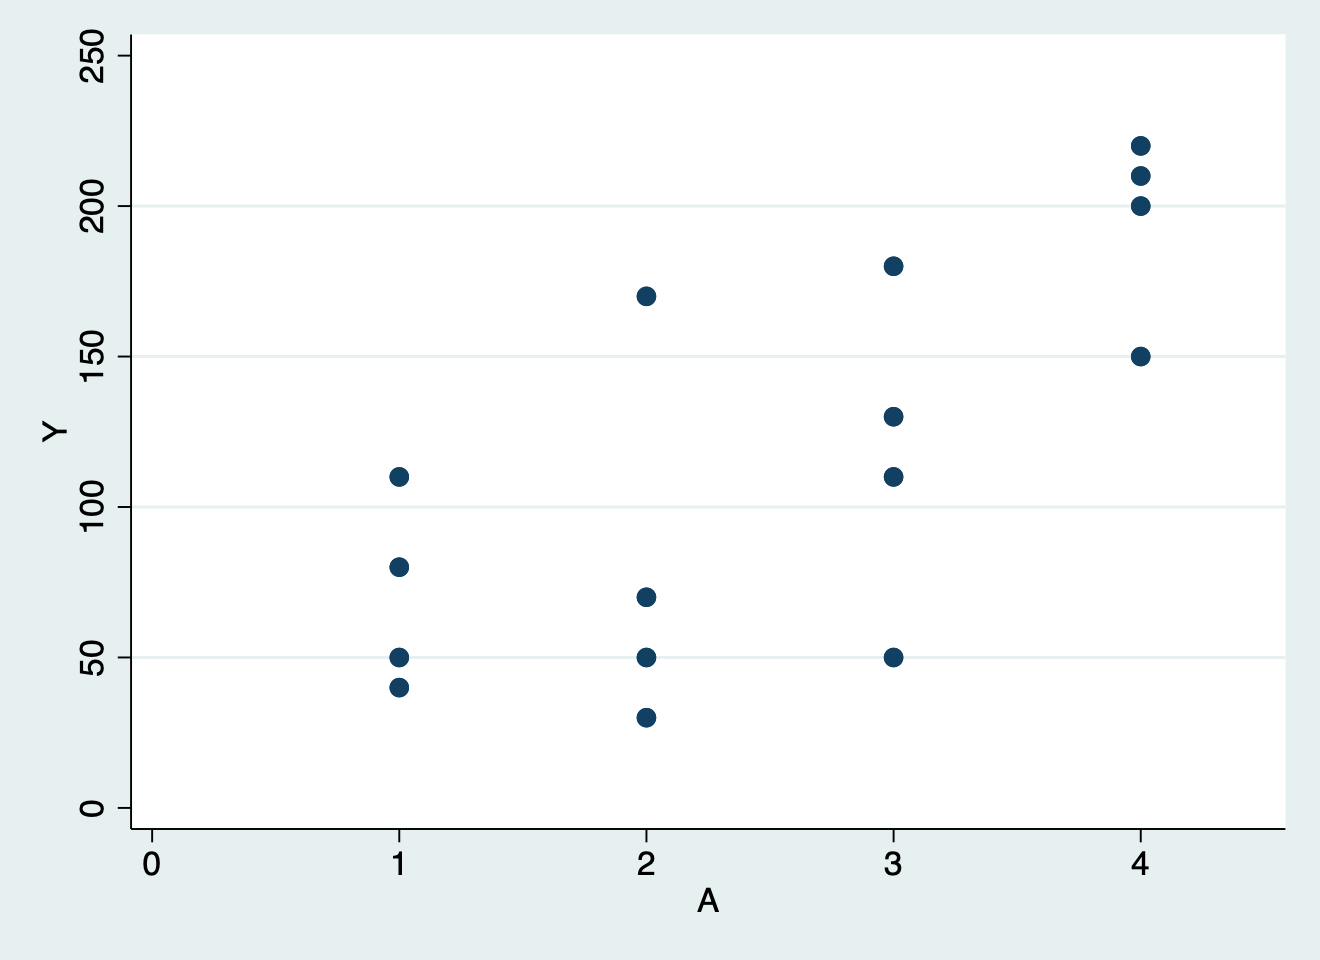
\includegraphics[width=0.85\linewidth]{figs/stata-fig-11-2} \end{center}

\begin{Shaded}
\begin{Highlighting}[]
\KeywordTok{clear}

\NormalTok{**Figure 11.3**}
\NormalTok{input A Y}
\NormalTok{3   21  }
\NormalTok{11  54}
\NormalTok{17  33}
\NormalTok{23  101}
\NormalTok{29  85}
\NormalTok{37  65}
\NormalTok{41  157}
\NormalTok{53  120}
\NormalTok{67  111}
\NormalTok{79  200}
\NormalTok{83  140}
\NormalTok{97  220}
\NormalTok{60  230}
\NormalTok{71  217}
\NormalTok{15  11}
\NormalTok{45  190}
\KeywordTok{end}

\KeywordTok{qui} \KeywordTok{save}\NormalTok{ ./}\KeywordTok{data}\NormalTok{/fig3, }\KeywordTok{replace}

\KeywordTok{scatter}\NormalTok{ Y A, ylab(0(50)250) xlab(0(10)100) }\BaseNTok{xscale}\NormalTok{(}\KeywordTok{range}\NormalTok{(0 100))}
\KeywordTok{qui} \KeywordTok{gr} \KeywordTok{export}\NormalTok{ figs/stata{-}fig{-}11{-}3.png, }\KeywordTok{replace}
\end{Highlighting}
\end{Shaded}

\begin{verbatim}
             A          Y
  1. 3   21  
  2. 11      54
  3. 17      33
  4. 23      101
  5. 29      85
  6. 37      65
  7. 41      157
  8. 53      120
  9. 67      111
 10. 79      200
 11. 83      140
 12. 97      220
 13. 60      230
 14. 71      217
 15. 15      11
 16. 45  190
 17. end
\end{verbatim}

\begin{center}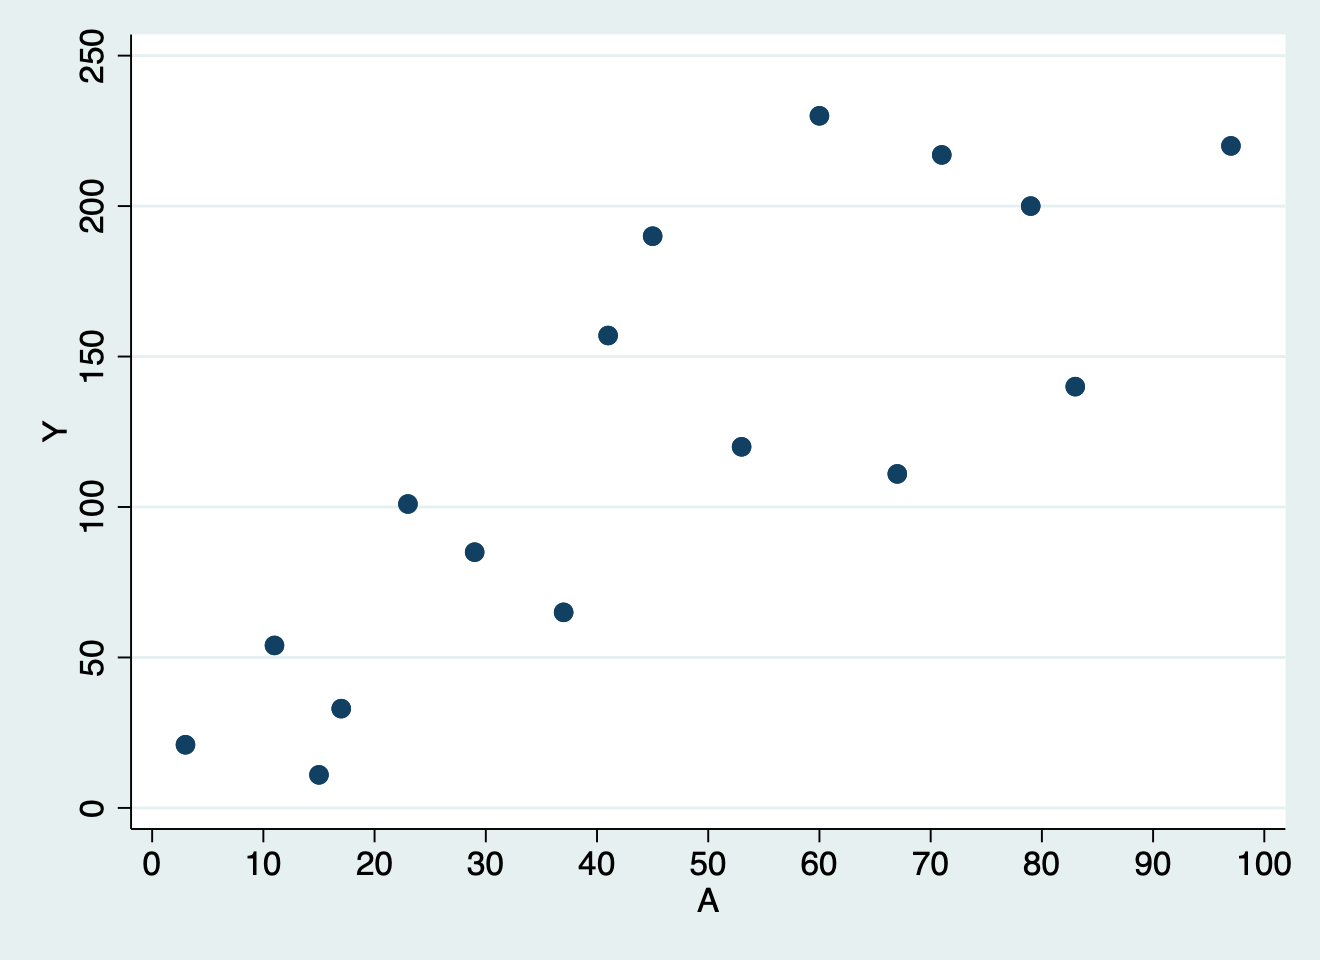
\includegraphics[width=0.85\linewidth]{figs/stata-fig-11-3} \end{center}

\hypertarget{program-11.2-1}{%
\section{Program 11.2}\label{program-11.2-1}}

\begin{itemize}
\tightlist
\item
  2-parameter linear model
\item
  Creates Figure 11.4, parameter estimates with 95\% confidence intervals from Section 11.2, and parameter estimates with 95\% confidence intervals from Section 11.3
\end{itemize}

\begin{Shaded}
\begin{Highlighting}[]
\NormalTok{**Section 11.2: parametric estimators**}
\NormalTok{*Reload }\KeywordTok{data}
\KeywordTok{use}\NormalTok{ ./}\KeywordTok{data}\NormalTok{/fig3, }\KeywordTok{clear}

\NormalTok{*Plot the }\KeywordTok{data}\NormalTok{*}
\KeywordTok{scatter}\NormalTok{ Y A, ylab(0(50)250) xlab(0(10)100) }\BaseNTok{xscale}\NormalTok{(}\KeywordTok{range}\NormalTok{(0 100))}

\NormalTok{*Fit the regression }\KeywordTok{model}\NormalTok{*}
\KeywordTok{regress}\NormalTok{ Y A, }\KeywordTok{noheader}\NormalTok{ cformat(\%5.2f)}

\NormalTok{*Output the estimated }\KeywordTok{mean}\NormalTok{ Y }\OtherTok{value}\NormalTok{ when A = 90*}
\KeywordTok{lincom}\NormalTok{ \_b[}\DataTypeTok{\_cons}\NormalTok{] + 90*\_b[A]}

\NormalTok{*Plot the }\KeywordTok{data}\NormalTok{ with the regression }\KeywordTok{line}\NormalTok{: Fig 11.4*}
\KeywordTok{scatter}\NormalTok{ Y A, ylab(0(50)250) xlab(0(10)100) }\BaseNTok{xscale}\NormalTok{(}\KeywordTok{range}\NormalTok{(0 100)) || }\KeywordTok{lfit}\NormalTok{ Y A}
\KeywordTok{qui} \KeywordTok{gr} \KeywordTok{export}\NormalTok{ figs/stata{-}fig{-}11{-}4.png, }\KeywordTok{replace}
\end{Highlighting}
\end{Shaded}

\begin{verbatim}
           Y | Coefficient  Std. err.      t    P>|t|     [95% conf. interval]
-------------+----------------------------------------------------------------
           A |       2.14       0.40     5.35   0.000         1.28        2.99
       _cons |      24.55      21.33     1.15   0.269       -21.20       70.29
------------------------------------------------------------------------------


 ( 1)  90*A + _cons = 0

------------------------------------------------------------------------------
           Y | Coefficient  Std. err.      t    P>|t|     [95% conf. interval]
-------------+----------------------------------------------------------------
         (1) |     216.89    20.8614    10.40   0.000     172.1468    261.6333
------------------------------------------------------------------------------
\end{verbatim}

\begin{center}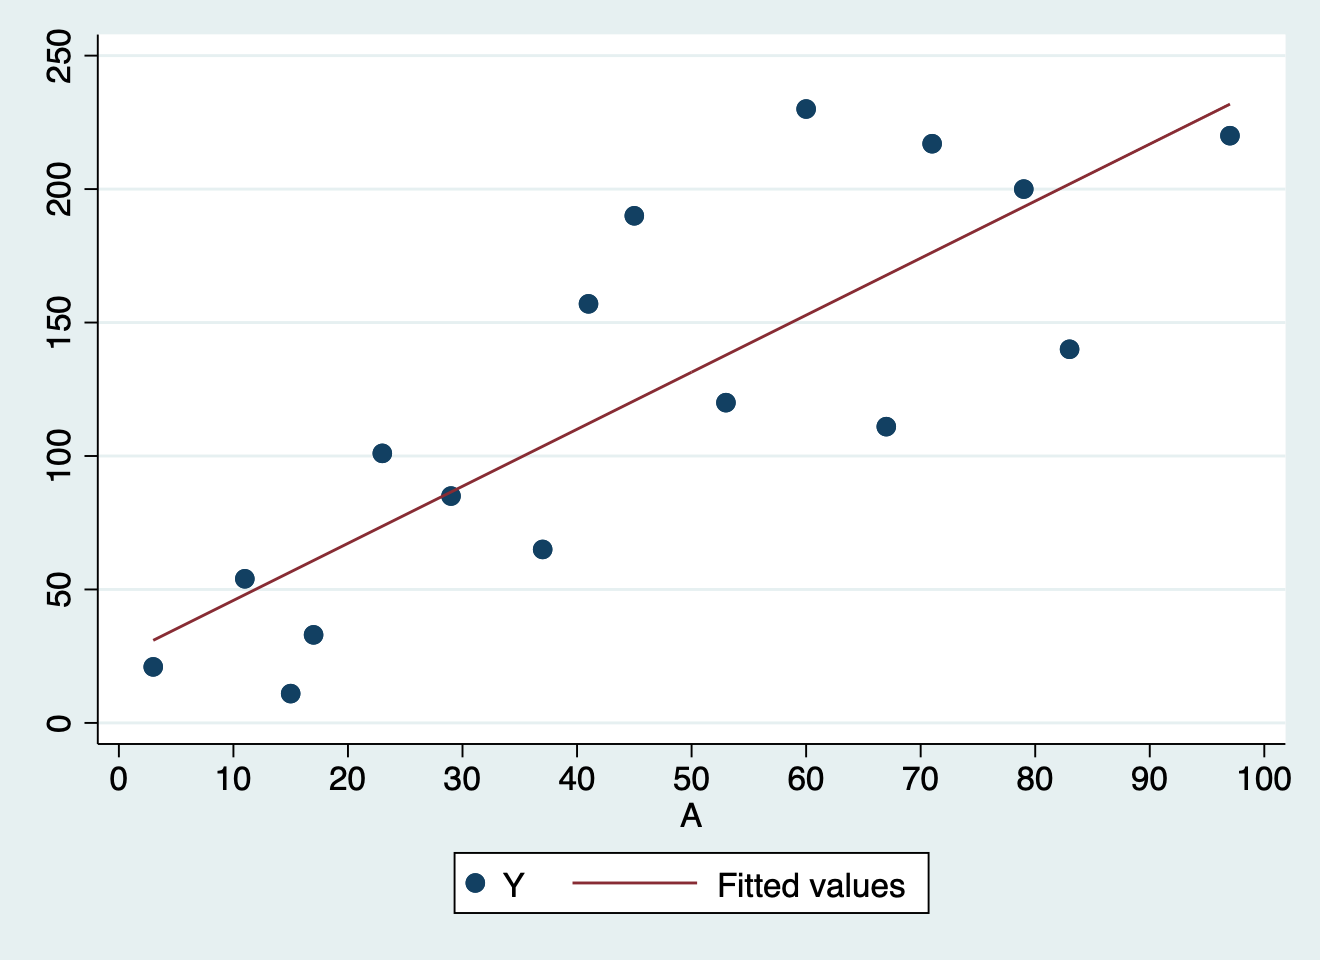
\includegraphics[width=0.85\linewidth]{figs/stata-fig-11-4} \end{center}

\begin{Shaded}
\begin{Highlighting}[]
\NormalTok{**Section 11.3: non{-}parametric estimation*}
\NormalTok{* Reload the }\KeywordTok{data}
\KeywordTok{use}\NormalTok{ ./}\KeywordTok{data}\NormalTok{/fig1, }\KeywordTok{clear}

\NormalTok{*Fit the regression }\KeywordTok{model}\NormalTok{*}
\KeywordTok{regress}\NormalTok{ Y A, }\KeywordTok{noheader}\NormalTok{ cformat(\%5.2f)}

\NormalTok{*E[Y|A=1]*}
\KeywordTok{di}\NormalTok{ 67.50 + 78.75}
\end{Highlighting}
\end{Shaded}

\begin{verbatim}
           Y | Coefficient  Std. err.      t    P>|t|     [95% conf. interval]
-------------+----------------------------------------------------------------
           A |      78.75      27.88     2.82   0.014        18.95      138.55
       _cons |      67.50      19.72     3.42   0.004        25.21      109.79
------------------------------------------------------------------------------

146.25
\end{verbatim}

\hypertarget{program-11.3-1}{%
\section{Program 11.3}\label{program-11.3-1}}

\begin{itemize}
\tightlist
\item
  3-parameter linear model
\item
  Creates Figure 11.5 and Parameter estimates for Section 11.4
\end{itemize}

\begin{Shaded}
\begin{Highlighting}[]
\NormalTok{* Reload the }\KeywordTok{data}
\KeywordTok{use}\NormalTok{ ./}\KeywordTok{data}\NormalTok{/fig3, }\KeywordTok{clear}

\NormalTok{*Create the product term*}
\KeywordTok{gen}\NormalTok{ Asq = A*A}

\NormalTok{*Fit the regression }\KeywordTok{model}\NormalTok{*}
\KeywordTok{regress}\NormalTok{ Y A Asq, }\KeywordTok{noheader}\NormalTok{ cformat(\%5.2f)}

\NormalTok{*Output the estimated }\KeywordTok{mean}\NormalTok{ Y }\OtherTok{value}\NormalTok{ when A = 90*}
\KeywordTok{lincom}\NormalTok{ \_b[}\DataTypeTok{\_cons}\NormalTok{] + 90*\_b[A] + 90*90*\_b[Asq]}

\NormalTok{*Plot the }\KeywordTok{data}\NormalTok{ with the regression }\KeywordTok{line}\NormalTok{: Fig 11.5*}
\KeywordTok{scatter}\NormalTok{ Y A, ylab(0(50)250) xlab(0(10)100) }\BaseNTok{xscale}\NormalTok{(}\KeywordTok{range}\NormalTok{(0 100)) || qfit Y A}
\KeywordTok{qui} \KeywordTok{gr} \KeywordTok{export}\NormalTok{ figs/stata{-}fig{-}11{-}5.png, }\KeywordTok{replace}
\end{Highlighting}
\end{Shaded}

\begin{verbatim}
           Y | Coefficient  Std. err.      t    P>|t|     [95% conf. interval]
-------------+----------------------------------------------------------------
           A |       4.11       1.53     2.68   0.019         0.80        7.41
         Asq |      -0.02       0.02    -1.33   0.206        -0.05        0.01
       _cons |      -7.41      31.75    -0.23   0.819       -75.99       61.18
------------------------------------------------------------------------------


 ( 1)  90*A + 8100*Asq + _cons = 0

------------------------------------------------------------------------------
           Y | Coefficient  Std. err.      t    P>|t|     [95% conf. interval]
-------------+----------------------------------------------------------------
         (1) |   197.1269   25.16157     7.83   0.000     142.7687    251.4852
------------------------------------------------------------------------------
\end{verbatim}

\begin{center}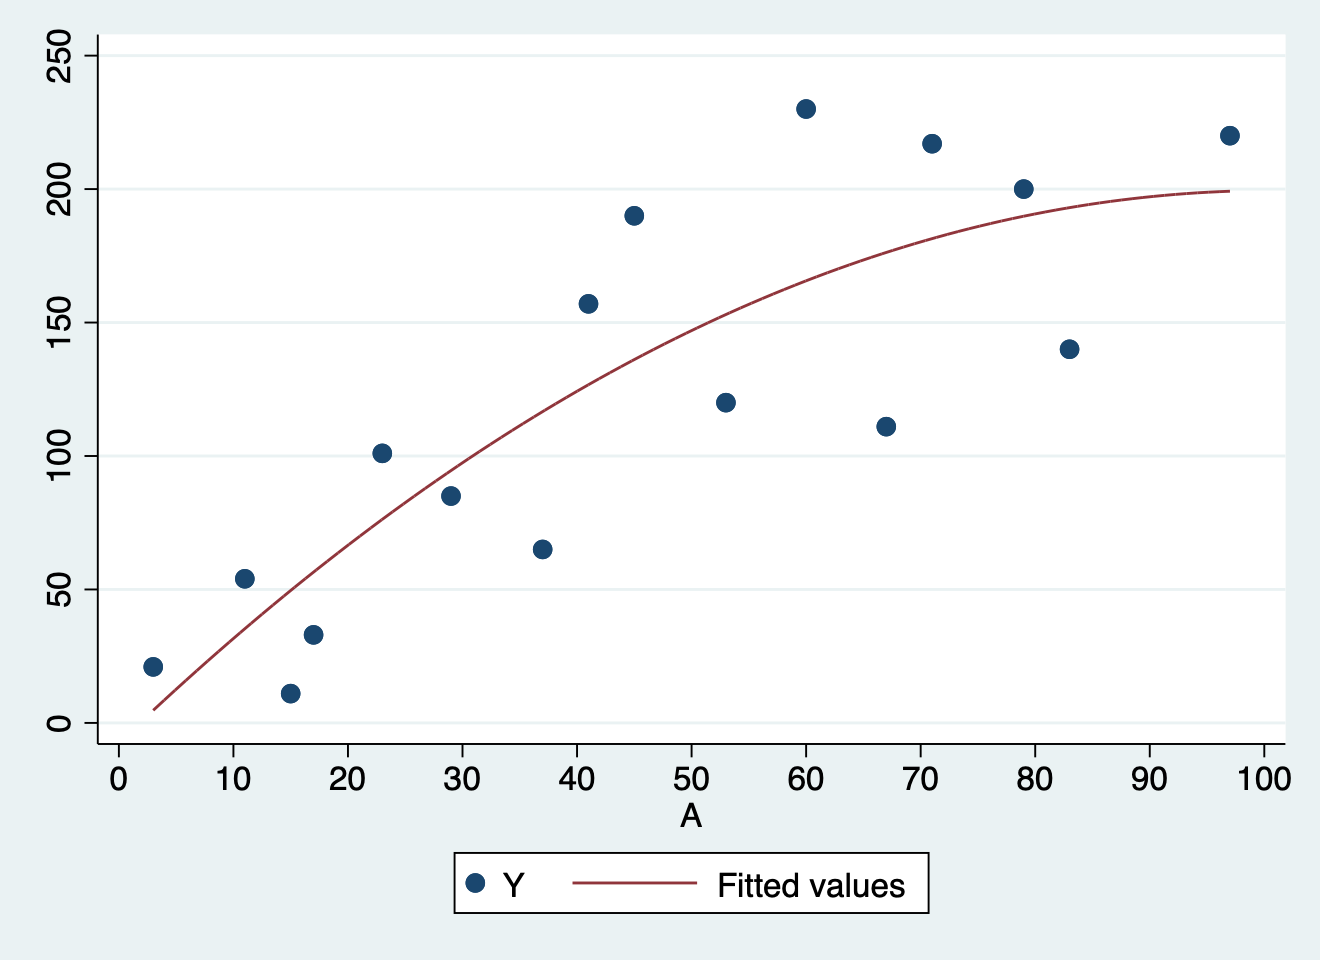
\includegraphics[width=0.85\linewidth]{figs/stata-fig-11-5} \end{center}

\hypertarget{ip-weighting-and-marginal-structural-models-stata}{%
\chapter*{12. IP Weighting and Marginal Structural Models: Stata}\label{ip-weighting-and-marginal-structural-models-stata}}
\addcontentsline{toc}{chapter}{12. IP Weighting and Marginal Structural Models: Stata}

\begin{Shaded}
\begin{Highlighting}[]
\FunctionTok{library}\NormalTok{(Statamarkdown)}
\end{Highlighting}
\end{Shaded}

\begin{verbatim}
/***************************************************************
Stata code for Causal Inference: What If by Miguel Hernan & Jamie Robins
Date: 10/10/2019
Author: Eleanor Murray 
For errors contact: ejmurray@bu.edu
***************************************************************/
\end{verbatim}

\hypertarget{program-12.1-1}{%
\section{Program 12.1}\label{program-12.1-1}}

\begin{itemize}
\tightlist
\item
  Descriptive statistics from NHEFS data (Table 12.1)
\end{itemize}

\begin{Shaded}
\begin{Highlighting}[]
\KeywordTok{use}\NormalTok{ ./}\KeywordTok{data}\NormalTok{/nhefs, }\KeywordTok{clear}

\CommentTok{/*Provisionally ignore subjects with missing values for follow{-}up weight*/}
\CommentTok{/*Sample size after exclusion: N = 1566*/}
\KeywordTok{drop} \KeywordTok{if}\NormalTok{ wt82==.}

\CommentTok{/* Calculate mean weight change in those with and without smoking cessation*/}
\KeywordTok{label} \KeywordTok{define}\NormalTok{ qsmk 0 }\StringTok{"No smoking cessation"}\NormalTok{ 1 }\StringTok{"Smoking cessation"}
\KeywordTok{label} \KeywordTok{values}\NormalTok{ qsmk qsmk}
\KeywordTok{by}\NormalTok{ qsmk, }\KeywordTok{sort}\NormalTok{: }\KeywordTok{egen}\NormalTok{ years = }\KeywordTok{mean}\NormalTok{(age) }\KeywordTok{if}\NormalTok{ age \textless{} . }
\KeywordTok{label} \KeywordTok{var}\NormalTok{ years }\StringTok{"Age, years"}
\KeywordTok{by}\NormalTok{ qsmk, }\KeywordTok{sort}\NormalTok{: }\KeywordTok{egen}\NormalTok{ male = }\KeywordTok{mean}\NormalTok{(100 * (sex==0)) }\KeywordTok{if}\NormalTok{ sex \textless{} . }
\KeywordTok{label} \KeywordTok{var}\NormalTok{ male }\StringTok{"Men, \%"}
\KeywordTok{by}\NormalTok{ qsmk, }\KeywordTok{sort}\NormalTok{: }\KeywordTok{egen} \BaseNTok{white}\NormalTok{ = }\KeywordTok{mean}\NormalTok{(100 * (race==0)) }\KeywordTok{if}\NormalTok{ race \textless{} . }
\KeywordTok{label} \KeywordTok{var} \BaseNTok{white} \StringTok{"White, \%"}
\KeywordTok{by}\NormalTok{ qsmk, }\KeywordTok{sort}\NormalTok{: }\KeywordTok{egen}\NormalTok{ university = }\KeywordTok{mean}\NormalTok{(100 * (education == 5)) }\KeywordTok{if}\NormalTok{ education \textless{} .}
\KeywordTok{label} \KeywordTok{var}\NormalTok{ university }\StringTok{"University, \%"}
\KeywordTok{by}\NormalTok{ qsmk, }\KeywordTok{sort}\NormalTok{: }\KeywordTok{egen}\NormalTok{ kg = }\KeywordTok{mean}\NormalTok{(wt71) }\KeywordTok{if}\NormalTok{ wt71 \textless{} .}
\KeywordTok{label} \KeywordTok{var}\NormalTok{ kg }\StringTok{"Weight, kg"}
\KeywordTok{by}\NormalTok{ qsmk, }\KeywordTok{sort}\NormalTok{: }\KeywordTok{egen}\NormalTok{ cigs = }\KeywordTok{mean}\NormalTok{(smokeintensity) }\KeywordTok{if}\NormalTok{ smokeintensity \textless{} . }
\KeywordTok{label} \KeywordTok{var}\NormalTok{ cigs }\StringTok{"Cigarettes/day"}
\KeywordTok{by}\NormalTok{ qsmk, }\KeywordTok{sort}\NormalTok{: }\KeywordTok{egen}\NormalTok{ meansmkyrs = }\KeywordTok{mean}\NormalTok{(smokeyrs) }\KeywordTok{if}\NormalTok{ smokeyrs \textless{} .}
\KeywordTok{label} \KeywordTok{var}\NormalTok{ kg }\StringTok{"Years smoking"}
\KeywordTok{by}\NormalTok{ qsmk, }\KeywordTok{sort}\NormalTok{: }\KeywordTok{egen}\NormalTok{ noexer = }\KeywordTok{mean}\NormalTok{(100 * (exercise == 2)) }\KeywordTok{if}\NormalTok{ exercise \textless{} . }
\KeywordTok{label} \KeywordTok{var}\NormalTok{ noexer }\StringTok{"Little/no exercise"}
\KeywordTok{by}\NormalTok{ qsmk, }\KeywordTok{sort}\NormalTok{: }\KeywordTok{egen}\NormalTok{ inactive = }\KeywordTok{mean}\NormalTok{(100 * (active==2)) }\KeywordTok{if}\NormalTok{ active \textless{} . }
\KeywordTok{label} \KeywordTok{var}\NormalTok{ inactive }\StringTok{"Inactive daily life"}
\KeywordTok{qui} \KeywordTok{save}\NormalTok{ ./}\KeywordTok{data}\NormalTok{/nhefs{-}formatted, }\KeywordTok{replace}
\end{Highlighting}
\end{Shaded}

\begin{verbatim}
(63 observations deleted)
\end{verbatim}

\begin{Shaded}
\begin{Highlighting}[]
\KeywordTok{use}\NormalTok{ ./}\KeywordTok{data}\NormalTok{/nhefs{-}formatted, }\KeywordTok{clear}

\CommentTok{/*Output table*/}
\KeywordTok{foreach} \KeywordTok{var} \KeywordTok{of} \KeywordTok{varlist}\NormalTok{ years male  }\BaseNTok{white}\NormalTok{ university kg cigs meansmkyrs noexer inactive \{}
\NormalTok{  tabdisp qsmk, cell(}\OtherTok{\textasciigrave{}var\textquotesingle{}}\NormalTok{) }\KeywordTok{format}\NormalTok{(\%3.1f)}
\NormalTok{\}}
\end{Highlighting}
\end{Shaded}

\begin{verbatim}
  2.   tabdisp qsmk, cell(`var') format(%3.1f)
  3. }

---------------------------------
quit smoking between |
baseline and 1982    | Age, years
---------------------+-----------
No smoking cessation |       42.8
   Smoking cessation |       46.2
---------------------------------

---------------------------------
quit smoking between |
baseline and 1982    |     Men, %
---------------------+-----------
No smoking cessation |       46.6
   Smoking cessation |       54.6
---------------------------------

---------------------------------
quit smoking between |
baseline and 1982    |   White, %
---------------------+-----------
No smoking cessation |       85.4
   Smoking cessation |       91.1
---------------------------------

------------------------------------
quit smoking between |
baseline and 1982    | University, %
---------------------+--------------
No smoking cessation |           9.9
   Smoking cessation |          15.4
------------------------------------

------------------------------------
quit smoking between |
baseline and 1982    | Years smoking
---------------------+--------------
No smoking cessation |          70.3
   Smoking cessation |          72.4
------------------------------------

-------------------------------------
quit smoking between |
baseline and 1982    | Cigarettes/day
---------------------+---------------
No smoking cessation |           21.2
   Smoking cessation |           18.6
-------------------------------------

---------------------------------
quit smoking between |
baseline and 1982    | meansmkyrs
---------------------+-----------
No smoking cessation |       24.1
   Smoking cessation |       26.0
---------------------------------

-----------------------------------------
quit smoking between |
baseline and 1982    | Little/no exercise
---------------------+-------------------
No smoking cessation |               37.9
   Smoking cessation |               40.7
-----------------------------------------

------------------------------------------
quit smoking between |
baseline and 1982    | Inactive daily life
---------------------+--------------------
No smoking cessation |                 8.9
   Smoking cessation |                11.2
------------------------------------------
\end{verbatim}

\hypertarget{program-12.2-1}{%
\section{Program 12.2}\label{program-12.2-1}}

\begin{itemize}
\tightlist
\item
  Estimating IP weights for Section 12.2
\item
  Data from NHEFS
\end{itemize}

\begin{Shaded}
\begin{Highlighting}[]
\KeywordTok{use}\NormalTok{ ./}\KeywordTok{data}\NormalTok{/nhefs{-}formatted, }\KeywordTok{clear}

\CommentTok{/*Fit a logistic model for the IP weights*/} 
\KeywordTok{logit}\NormalTok{ qsmk sex race c.age\#\#c.age ib(}\FunctionTok{last}\NormalTok{).education c.smokeintensity\#\#c.smokeintensity }\CommentTok{///}
\NormalTok{c.smokeyrs\#\#c.smokeyrs ib(}\FunctionTok{last}\NormalTok{).exercise ib(}\FunctionTok{last}\NormalTok{).active c.wt71\#\#c.wt71 }

\CommentTok{/*Output predicted conditional probability of quitting smoking for each individual*/}
\KeywordTok{predict}\NormalTok{ p\_qsmk, pr}

\CommentTok{/*Generate nonstabilized weights as P(A=1|covariates) if A = 1 and 1{-}P(A=1|covariates) if A = 0*/}
\KeywordTok{gen} \FunctionTok{w}\NormalTok{=.}
\KeywordTok{replace} \FunctionTok{w}\NormalTok{=1/p\_qsmk }\KeywordTok{if}\NormalTok{ qsmk==1}
\KeywordTok{replace} \FunctionTok{w}\NormalTok{=1/(1{-}p\_qsmk) }\KeywordTok{if}\NormalTok{ qsmk==0}
\CommentTok{/*Check the mean of the weights; we expect it to be close to 2.0*/}
\KeywordTok{summarize} \FunctionTok{w}

\CommentTok{/*Fit marginal structural model in the pseudopopulation*/}
\CommentTok{/*Weights assigned using pweight = w*/}
\CommentTok{/*Robust standard errors using cluster() option where \textquotesingle{}seqn\textquotesingle{} is the ID variable*/}
\KeywordTok{regress}\NormalTok{ wt82\_71 qsmk [}\KeywordTok{pweight}\NormalTok{=}\FunctionTok{w}\NormalTok{], }\KeywordTok{cluster}\NormalTok{(seqn) }
\end{Highlighting}
\end{Shaded}

\begin{verbatim}
Iteration 0:   log likelihood = -893.02712  
Iteration 1:   log likelihood = -839.70016  
Iteration 2:   log likelihood = -838.45045  
Iteration 3:   log likelihood = -838.44842  
Iteration 4:   log likelihood = -838.44842  

Logistic regression                                     Number of obs =  1,566
                                                        LR chi2(18)   = 109.16
                                                        Prob > chi2   = 0.0000
Log likelihood = -838.44842                             Pseudo R2     = 0.0611

-------------------------------------------------------------------------------
         qsmk | Coefficient  Std. err.      z    P>|z|     [95% conf. interval]
--------------+----------------------------------------------------------------
          sex |  -.5274782   .1540497    -3.42   0.001      -.82941   -.2255463
         race |  -.8392636   .2100668    -4.00   0.000    -1.250987   -.4275404
          age |   .1212052   .0512663     2.36   0.018     .0207251    .2216853
              |
  c.age#c.age |  -.0008246   .0005361    -1.54   0.124    -.0018753    .0002262
              |
    education |
           1  |  -.4759606   .2262238    -2.10   0.035    -.9193511   -.0325701
           2  |  -.5047361    .217597    -2.32   0.020    -.9312184   -.0782538
           3  |  -.3895288   .1914353    -2.03   0.042    -.7647351   -.0143226
           4  |  -.4123596   .2772868    -1.49   0.137    -.9558318    .1311126
              |
smokeintens~y |  -.0772704   .0152499    -5.07   0.000    -.1071596   -.0473812
              |
           c. |
smokeintens~y#|
           c. |
smokeintens~y |   .0010451   .0002866     3.65   0.000     .0004835    .0016068
              |
     smokeyrs |  -.0735966   .0277775    -2.65   0.008    -.1280395   -.0191538
              |
   c.smokeyrs#|
   c.smokeyrs |   .0008441   .0004632     1.82   0.068    -.0000637    .0017519
              |
     exercise |
           0  |   -.395704   .1872401    -2.11   0.035    -.7626878   -.0287201
           1  |  -.0408635   .1382674    -0.30   0.768    -.3118627    .2301357
              |
       active |
           0  |   -.176784   .2149721    -0.82   0.411    -.5981215    .2445535
           1  |  -.1448395   .2111472    -0.69   0.493    -.5586806    .2690015
              |
         wt71 |  -.0152357   .0263161    -0.58   0.563    -.0668144     .036343
              |
c.wt71#c.wt71 |   .0001352   .0001632     0.83   0.407    -.0001846     .000455
              |
        _cons |   -1.19407   1.398493    -0.85   0.393    -3.935066    1.546925
-------------------------------------------------------------------------------


(1,566 missing values generated)

(403 real changes made)

(1,163 real changes made)

    Variable |        Obs        Mean    Std. dev.       Min        Max
-------------+---------------------------------------------------------
           w |      1,566    1.996284    1.474787   1.053742   16.70009

(sum of wgt is 3,126.18084549904)

Linear regression                               Number of obs     =      1,566
                                                F(1, 1565)        =      42.81
                                                Prob > F          =     0.0000
                                                R-squared         =     0.0435
                                                Root MSE          =     8.0713

                               (Std. err. adjusted for 1,566 clusters in seqn)
------------------------------------------------------------------------------
             |               Robust
     wt82_71 | Coefficient  std. err.      t    P>|t|     [95% conf. interval]
-------------+----------------------------------------------------------------
        qsmk |   3.440535   .5258294     6.54   0.000     2.409131     4.47194
       _cons |   1.779978   .2248742     7.92   0.000     1.338892    2.221065
------------------------------------------------------------------------------
\end{verbatim}

\hypertarget{program-12.3-1}{%
\section{Program 12.3}\label{program-12.3-1}}

\begin{itemize}
\tightlist
\item
  Estimating stabilized IP weights for Section 12.3
\item
  Data from NHEFS
\end{itemize}

\begin{Shaded}
\begin{Highlighting}[]
\KeywordTok{use}\NormalTok{ ./}\KeywordTok{data}\NormalTok{/nhefs{-}formatted, }\KeywordTok{clear}

\CommentTok{/*Fit a logistic model for the denominator of the IP weights and predict the conditional probability of smoking*/} 
\KeywordTok{logit}\NormalTok{ qsmk sex race c.age\#\#c.age ib(}\FunctionTok{last}\NormalTok{).education c.smokeintensity\#\#c.smokeintensity }\CommentTok{///}
\NormalTok{c.smokeyrs\#\#c.smokeyrs ib(}\FunctionTok{last}\NormalTok{).exercise ib(}\FunctionTok{last}\NormalTok{).active c.wt71\#\#c.wt71  }
\KeywordTok{predict}\NormalTok{ pd\_qsmk, pr}

\CommentTok{/*Fit a logistic model for the numerator of ip weights and predict Pr(A=1) */} 
\KeywordTok{logit}\NormalTok{ qsmk }
\KeywordTok{predict}\NormalTok{ pn\_qsmk, pr}

\CommentTok{/*Generate stabilized weights as f(A)/f(A|L)*/}
\KeywordTok{gen}\NormalTok{ sw\_a=.}
\KeywordTok{replace}\NormalTok{ sw\_a=pn\_qsmk/pd\_qsmk }\KeywordTok{if}\NormalTok{ qsmk==1}
\KeywordTok{replace}\NormalTok{ sw\_a=(1{-}pn\_qsmk)/(1{-}pd\_qsmk) }\KeywordTok{if}\NormalTok{ qsmk==0}

\CommentTok{/*Check distribution of the stabilized weights*/}
\KeywordTok{summarize}\NormalTok{ sw\_a}

\CommentTok{/*Fit marginal structural model in the pseudopopulation*/}
\KeywordTok{regress}\NormalTok{ wt82\_71 qsmk [}\KeywordTok{pweight}\NormalTok{=sw\_a], }\KeywordTok{cluster}\NormalTok{(seqn) }

\CommentTok{/**********************************************************}
\CommentTok{FINE POINT 12.2}
\CommentTok{Checking positivity}
\CommentTok{**********************************************************/}

\CommentTok{/*Check for missing values within strata of covariates, for example: */}
\KeywordTok{tab}\NormalTok{ age qsmk }\KeywordTok{if}\NormalTok{ race==0 \& sex==1 \& wt82!=.}
\KeywordTok{tab}\NormalTok{ age qsmk }\KeywordTok{if}\NormalTok{ race==1 \& sex==1 \& wt82!=.}
\end{Highlighting}
\end{Shaded}

\begin{verbatim}
Iteration 0:   log likelihood = -893.02712  
Iteration 1:   log likelihood = -839.70016  
Iteration 2:   log likelihood = -838.45045  
Iteration 3:   log likelihood = -838.44842  
Iteration 4:   log likelihood = -838.44842  

Logistic regression                                     Number of obs =  1,566
                                                        LR chi2(18)   = 109.16
                                                        Prob > chi2   = 0.0000
Log likelihood = -838.44842                             Pseudo R2     = 0.0611

-------------------------------------------------------------------------------
         qsmk | Coefficient  Std. err.      z    P>|z|     [95% conf. interval]
--------------+----------------------------------------------------------------
          sex |  -.5274782   .1540497    -3.42   0.001      -.82941   -.2255463
         race |  -.8392636   .2100668    -4.00   0.000    -1.250987   -.4275404
          age |   .1212052   .0512663     2.36   0.018     .0207251    .2216853
              |
  c.age#c.age |  -.0008246   .0005361    -1.54   0.124    -.0018753    .0002262
              |
    education |
           1  |  -.4759606   .2262238    -2.10   0.035    -.9193511   -.0325701
           2  |  -.5047361    .217597    -2.32   0.020    -.9312184   -.0782538
           3  |  -.3895288   .1914353    -2.03   0.042    -.7647351   -.0143226
           4  |  -.4123596   .2772868    -1.49   0.137    -.9558318    .1311126
              |
smokeintens~y |  -.0772704   .0152499    -5.07   0.000    -.1071596   -.0473812
              |
           c. |
smokeintens~y#|
           c. |
smokeintens~y |   .0010451   .0002866     3.65   0.000     .0004835    .0016068
              |
     smokeyrs |  -.0735966   .0277775    -2.65   0.008    -.1280395   -.0191538
              |
   c.smokeyrs#|
   c.smokeyrs |   .0008441   .0004632     1.82   0.068    -.0000637    .0017519
              |
     exercise |
           0  |   -.395704   .1872401    -2.11   0.035    -.7626878   -.0287201
           1  |  -.0408635   .1382674    -0.30   0.768    -.3118627    .2301357
              |
       active |
           0  |   -.176784   .2149721    -0.82   0.411    -.5981215    .2445535
           1  |  -.1448395   .2111472    -0.69   0.493    -.5586806    .2690015
              |
         wt71 |  -.0152357   .0263161    -0.58   0.563    -.0668144     .036343
              |
c.wt71#c.wt71 |   .0001352   .0001632     0.83   0.407    -.0001846     .000455
              |
        _cons |   -1.19407   1.398493    -0.85   0.393    -3.935066    1.546925
-------------------------------------------------------------------------------



Iteration 0:   log likelihood = -893.02712  
Iteration 1:   log likelihood = -893.02712  

Logistic regression                                     Number of obs =  1,566
                                                        LR chi2(0)    =   0.00
                                                        Prob > chi2   =      .
Log likelihood = -893.02712                             Pseudo R2     = 0.0000

------------------------------------------------------------------------------
        qsmk | Coefficient  Std. err.      z    P>|z|     [95% conf. interval]
-------------+----------------------------------------------------------------
       _cons |  -1.059822   .0578034   -18.33   0.000    -1.173114    -.946529
------------------------------------------------------------------------------


(1,566 missing values generated)

(403 real changes made)

(1,163 real changes made)

    Variable |        Obs        Mean    Std. dev.       Min        Max
-------------+---------------------------------------------------------
        sw_a |      1,566    .9988444    .2882233   .3312489   4.297662

(sum of wgt is 1,564.19025221467)

Linear regression                               Number of obs     =      1,566
                                                F(1, 1565)        =      42.81
                                                Prob > F          =     0.0000
                                                R-squared         =     0.0359
                                                Root MSE          =     7.7972

                               (Std. err. adjusted for 1,566 clusters in seqn)
------------------------------------------------------------------------------
             |               Robust
     wt82_71 | Coefficient  std. err.      t    P>|t|     [95% conf. interval]
-------------+----------------------------------------------------------------
        qsmk |   3.440535   .5258294     6.54   0.000     2.409131     4.47194
       _cons |   1.779978   .2248742     7.92   0.000     1.338892    2.221065
------------------------------------------------------------------------------

           | quit smoking between
           |   baseline and 1982
       age | No smokin  Smoking c |     Total
-----------+----------------------+----------
        25 |        24          3 |        27 
        26 |        14          5 |        19 
        27 |        18          2 |        20 
        28 |        20          5 |        25 
        29 |        15          4 |        19 
        30 |        14          5 |        19 
        31 |        11          5 |        16 
        32 |        14          7 |        21 
        33 |        12          3 |        15 
        34 |        22          5 |        27 
        35 |        16          5 |        21 
        36 |        13          3 |        16 
        37 |        14          1 |        15 
        38 |         6          2 |         8 
        39 |        19          4 |        23 
        40 |        10          4 |        14 
        41 |        13          3 |        16 
        42 |        16          3 |        19 
        43 |        14          3 |        17 
        44 |         9          4 |        13 
        45 |        12          5 |        17 
        46 |        19          4 |        23 
        47 |        19          4 |        23 
        48 |        19          4 |        23 
        49 |        11          3 |        14 
        50 |        18          4 |        22 
        51 |         9          3 |        12 
        52 |        11          3 |        14 
        53 |        11          4 |        15 
        54 |        17          9 |        26 
        55 |         9          4 |        13 
        56 |         8          7 |        15 
        57 |         9          2 |        11 
        58 |         8          4 |        12 
        59 |         5          4 |         9 
        60 |         5          4 |         9 
        61 |         5          2 |         7 
        62 |         6          5 |        11 
        63 |         3          3 |         6 
        64 |         7          1 |         8 
        65 |         3          2 |         5 
        66 |         4          0 |         4 
        67 |         2          0 |         2 
        69 |         6          2 |         8 
        70 |         2          1 |         3 
        71 |         0          1 |         1 
        72 |         2          2 |         4 
        74 |         0          1 |         1 
-----------+----------------------+----------
     Total |       524        164 |       688 

           | quit smoking between
           |   baseline and 1982
       age | No smokin  Smoking c |     Total
-----------+----------------------+----------
        25 |         3          1 |         4 
        26 |         3          0 |         3 
        28 |         3          1 |         4 
        29 |         1          0 |         1 
        30 |         4          0 |         4 
        31 |         3          0 |         3 
        32 |         8          0 |         8 
        33 |         2          0 |         2 
        34 |         2          1 |         3 
        35 |         3          0 |         3 
        36 |         5          0 |         5 
        37 |         3          1 |         4 
        38 |         4          2 |         6 
        39 |         1          1 |         2 
        40 |         2          2 |         4 
        41 |         3          0 |         3 
        42 |         3          0 |         3 
        43 |         4          2 |         6 
        44 |         3          0 |         3 
        45 |         1          3 |         4 
        46 |         5          0 |         5 
        47 |         3          0 |         3 
        48 |         4          0 |         4 
        49 |         1          1 |         2 
        50 |         2          0 |         2 
        51 |         4          0 |         4 
        52 |         1          0 |         1 
        53 |         2          0 |         2 
        54 |         2          0 |         2 
        55 |         3          0 |         3 
        56 |         2          1 |         3 
        57 |         2          1 |         3 
        61 |         1          1 |         2 
        67 |         1          0 |         1 
        68 |         1          0 |         1 
        69 |         2          0 |         2 
        70 |         0          1 |         1 
-----------+----------------------+----------
     Total |        97         19 |       116 
\end{verbatim}

\hypertarget{program-12.4-1}{%
\section{Program 12.4}\label{program-12.4-1}}

\begin{itemize}
\tightlist
\item
  Estimating the parameters of a marginal structural mean model with a continuous treatment Data from NHEFS
\item
  Section 12.4
\end{itemize}

\begin{Shaded}
\begin{Highlighting}[]
\KeywordTok{use}\NormalTok{ ./}\KeywordTok{data}\NormalTok{/nhefs{-}formatted, }\KeywordTok{clear}

\NormalTok{* }\KeywordTok{drop}\NormalTok{ sw\_a}

\CommentTok{/*Analysis restricted to subjects reporting \textless{}=25 cig/day at baseline: N = 1162*/}
\KeywordTok{keep} \KeywordTok{if}\NormalTok{ smokeintensity \textless{}=25}

\CommentTok{/*Fit a linear model for the denominator of the IP weights and calculate the mean expected smoking intensity*/} 
\KeywordTok{regress}\NormalTok{ smkintensity82\_71 sex race c.age\#\#c.age ib(}\FunctionTok{last}\NormalTok{).education c.smokeintensity\#\#c.smokeintensity }\CommentTok{///}
\NormalTok{c.smokeyrs\#\#c.smokeyrs ib(}\FunctionTok{last}\NormalTok{).exercise ib(}\FunctionTok{last}\NormalTok{).active c.wt71\#\#c.wt71}
\KeywordTok{quietly} \KeywordTok{predict}\NormalTok{ p\_den}

\CommentTok{/*Generate the denisty of the denomiator expectation using the mean expected smoking intensity and the residuals, assuming a normal distribution*/}
\CommentTok{/*Note: The regress command in STATA saves the root mean squared error for the immediate regression as e(rmse), thus there is no need to calculate it again. */}
\KeywordTok{gen}\NormalTok{ dens\_den = }\FunctionTok{normalden}\NormalTok{(smkintensity82\_71, p\_den, }\FunctionTok{e}\NormalTok{(rmse))}

\CommentTok{/*Fit a linear model for the numerator of ip weights, calculate the mean expected value, and generate the density*/}
\KeywordTok{quietly} \KeywordTok{regress}\NormalTok{ smkintensity82\_71}
\KeywordTok{quietly} \KeywordTok{predict}\NormalTok{ p\_num}
\KeywordTok{gen}\NormalTok{ dens\_num = }\FunctionTok{normalden}\NormalTok{( smkintensity82\_71, p\_num, }\FunctionTok{e}\NormalTok{(rmse))}

\CommentTok{/*Generate the final stabilized weights from the estimated numerator and denominator, and check the weights distribution*/}
\KeywordTok{gen}\NormalTok{ sw\_a=dens\_num/dens\_den}
\KeywordTok{summarize}\NormalTok{ sw\_a}

\CommentTok{/*Fit a marginal structural model in the pseudopopulation*/}
\KeywordTok{regress}\NormalTok{ wt82\_71  c.smkintensity82\_71\#\#c.smkintensity82\_71 [}\KeywordTok{pweight}\NormalTok{=sw\_a], }\KeywordTok{cluster}\NormalTok{(seqn)}

\CommentTok{/*Output the estimated mean Y value when smoke intensity is unchanged from baseline to 1982 */}
\KeywordTok{lincom}\NormalTok{ \_b[}\DataTypeTok{\_cons}\NormalTok{]}

\CommentTok{/*Output the estimated mean Y value when smoke intensity increases by 20 from baseline to 1982*/}
\KeywordTok{lincom}\NormalTok{ \_b[}\DataTypeTok{\_cons}\NormalTok{] + 20*\_b[smkintensity82\_71 ] +400*\_b[c.smkintensity82\_71\#c.smkintensity82\_71]}
\end{Highlighting}
\end{Shaded}

\begin{verbatim}
(404 observations deleted)

      Source |       SS           df       MS      Number of obs   =     1,162
-------------+----------------------------------   F(18, 1143)     =      5.39
       Model |  9956.95654        18  553.164252   Prob > F        =    0.0000
    Residual |   117260.18     1,143  102.589834   R-squared       =    0.0783
-------------+----------------------------------   Adj R-squared   =    0.0638
       Total |  127217.137     1,161  109.575484   Root MSE        =    10.129

-------------------------------------------------------------------------------
smkintensi~71 | Coefficient  Std. err.      t    P>|t|     [95% conf. interval]
--------------+----------------------------------------------------------------
          sex |   1.087021   .7425694     1.46   0.144    -.3699308    2.543973
         race |   .2319789   .8434739     0.28   0.783    -1.422952     1.88691
          age |  -.8099902   .2555388    -3.17   0.002    -1.311368   -.3086124
              |
  c.age#c.age |   .0066545   .0026849     2.48   0.013     .0013865    .0119224
              |
    education |
           1  |   1.508097   1.184063     1.27   0.203    -.8150843    3.831278
           2  |    2.02692   1.133772     1.79   0.074    -.1975876    4.251428
           3  |   2.240314   1.022556     2.19   0.029     .2340167    4.246611
           4  |   2.528767    1.44702     1.75   0.081    -.3103458     5.36788
              |
smokeintens~y |  -.3589684   .2246653    -1.60   0.110     -.799771    .0818342
              |
           c. |
smokeintens~y#|
           c. |
smokeintens~y |   .0019582   .0085753     0.23   0.819    -.0148668    .0187832
              |
     smokeyrs |   .3857088   .1416765     2.72   0.007     .1077336    .6636841
              |
   c.smokeyrs#|
   c.smokeyrs |  -.0054871   .0023837    -2.30   0.022    -.0101641   -.0008101
              |
     exercise |
           0  |   1.996904   .9080421     2.20   0.028      .215288    3.778521
           1  |    .988812   .6929239     1.43   0.154    -.3707334    2.348357
              |
       active |
           0  |   .8451341   1.098573     0.77   0.442    -1.310312    3.000581
           1  |    .800114    1.08438     0.74   0.461    -1.327485    2.927712
              |
         wt71 |  -.0656882    .136955    -0.48   0.632    -.3343996    .2030232
              |
c.wt71#c.wt71 |   .0005711    .000877     0.65   0.515    -.0011496    .0022918
              |
        _cons |   16.86761   7.109189     2.37   0.018      2.91909    30.81614
-------------------------------------------------------------------------------

    Variable |        Obs        Mean    Std. dev.       Min        Max
-------------+---------------------------------------------------------
        sw_a |      1,162    .9968057    .3222937   .1938336   5.102339

(sum of wgt is 1,158.28818286955)

Linear regression                               Number of obs     =      1,162
                                                F(2, 1161)        =      12.75
                                                Prob > F          =     0.0000
                                                R-squared         =     0.0233
                                                Root MSE          =     7.7864

                                (Std. err. adjusted for 1,162 clusters in seqn)
-------------------------------------------------------------------------------
              |               Robust
      wt82_71 | Coefficient  std. err.      t    P>|t|     [95% conf. interval]
--------------+----------------------------------------------------------------
smkintensi~71 |  -.1089889   .0315762    -3.45   0.001    -.1709417   -.0470361
              |
           c. |
smkintensi~71#|
           c. |
smkintensi~71 |   .0026949   .0024203     1.11   0.266    -.0020537    .0074436
              |
        _cons |   2.004525    .295502     6.78   0.000     1.424747    2.584302
-------------------------------------------------------------------------------


 ( 1)  _cons = 0

------------------------------------------------------------------------------
     wt82_71 | Coefficient  Std. err.      t    P>|t|     [95% conf. interval]
-------------+----------------------------------------------------------------
         (1) |   2.004525    .295502     6.78   0.000     1.424747    2.584302
------------------------------------------------------------------------------


 ( 1)  20*smkintensity82_71 + 400*c.smkintensity82_71#c.smkintensity82_71 +
       _cons = 0

------------------------------------------------------------------------------
     wt82_71 | Coefficient  Std. err.      t    P>|t|     [95% conf. interval]
-------------+----------------------------------------------------------------
         (1) |   .9027234   1.310533     0.69   0.491    -1.668554    3.474001
------------------------------------------------------------------------------
\end{verbatim}

\hypertarget{program-12.5-1}{%
\section{Program 12.5}\label{program-12.5-1}}

\begin{itemize}
\tightlist
\item
  Estimating the parameters of a marginal structural logistic model
\item
  Data from NHEFS
\item
  Section 12.4
\end{itemize}

\begin{Shaded}
\begin{Highlighting}[]
\KeywordTok{use}\NormalTok{ ./}\KeywordTok{data}\NormalTok{/nhefs, }\KeywordTok{clear}

\CommentTok{/*Provisionally ignore subjects with missing values for follow{-}up weight*/}
\CommentTok{/*Sample size after exclusion: N = 1566*/}
\KeywordTok{drop} \KeywordTok{if}\NormalTok{ wt82==.}

\CommentTok{/*Estimate the stabilized weights for quitting smoking as in PROGRAM 12.3*/}
\CommentTok{/*Fit a logistic model for the denominator of the IP weights and predict the conditional probability of smoking*/} 
\KeywordTok{logit}\NormalTok{ qsmk sex race c.age\#\#c.age ib(}\FunctionTok{last}\NormalTok{).education c.smokeintensity\#\#c.smokeintensity }\CommentTok{///}
\NormalTok{c.smokeyrs\#\#c.smokeyrs ib(}\FunctionTok{last}\NormalTok{).exercise ib(}\FunctionTok{last}\NormalTok{).active c.wt71\#\#c.wt71  }
\KeywordTok{predict}\NormalTok{ pd\_qsmk, pr}
\CommentTok{/*Fit a logistic model for the numerator of ip weights and predict Pr(A=1) */} 
\KeywordTok{logit}\NormalTok{ qsmk }
\KeywordTok{predict}\NormalTok{ pn\_qsmk, pr}
\CommentTok{/*Generate stabilized weights as f(A)/f(A|L)*/}
\KeywordTok{gen}\NormalTok{ sw\_a=.}
\KeywordTok{replace}\NormalTok{ sw\_a=pn\_qsmk/pd\_qsmk }\KeywordTok{if}\NormalTok{ qsmk==1}
\KeywordTok{replace}\NormalTok{ sw\_a=(1{-}pn\_qsmk)/(1{-}pd\_qsmk) }\KeywordTok{if}\NormalTok{ qsmk==0}
\KeywordTok{summarize}\NormalTok{ sw\_a}

\CommentTok{/*Fit marginal structural model in the pseudopopulation*/}
\CommentTok{/*}\AlertTok{NOTE}\CommentTok{: Stata has two commands for logistic regression, logit and logistic*/}
\CommentTok{/*Using logistic allows us to output the odds ratios directly*/}
\CommentTok{/*We can also output odds ratios from the logit command using the or option (default logit output is regression coefficients*/}
\KeywordTok{logistic}\NormalTok{ death qsmk [}\KeywordTok{pweight}\NormalTok{=sw\_a], }\KeywordTok{cluster}\NormalTok{(seqn) }
\end{Highlighting}
\end{Shaded}

\begin{verbatim}
(63 observations deleted)


Iteration 0:   log likelihood = -893.02712  
Iteration 1:   log likelihood = -839.70016  
Iteration 2:   log likelihood = -838.45045  
Iteration 3:   log likelihood = -838.44842  
Iteration 4:   log likelihood = -838.44842  

Logistic regression                                     Number of obs =  1,566
                                                        LR chi2(18)   = 109.16
                                                        Prob > chi2   = 0.0000
Log likelihood = -838.44842                             Pseudo R2     = 0.0611

-------------------------------------------------------------------------------
         qsmk | Coefficient  Std. err.      z    P>|z|     [95% conf. interval]
--------------+----------------------------------------------------------------
          sex |  -.5274782   .1540497    -3.42   0.001      -.82941   -.2255463
         race |  -.8392636   .2100668    -4.00   0.000    -1.250987   -.4275404
          age |   .1212052   .0512663     2.36   0.018     .0207251    .2216853
              |
  c.age#c.age |  -.0008246   .0005361    -1.54   0.124    -.0018753    .0002262
              |
    education |
           1  |  -.4759606   .2262238    -2.10   0.035    -.9193511   -.0325701
           2  |  -.5047361    .217597    -2.32   0.020    -.9312184   -.0782538
           3  |  -.3895288   .1914353    -2.03   0.042    -.7647351   -.0143226
           4  |  -.4123596   .2772868    -1.49   0.137    -.9558318    .1311126
              |
smokeintens~y |  -.0772704   .0152499    -5.07   0.000    -.1071596   -.0473812
              |
           c. |
smokeintens~y#|
           c. |
smokeintens~y |   .0010451   .0002866     3.65   0.000     .0004835    .0016068
              |
     smokeyrs |  -.0735966   .0277775    -2.65   0.008    -.1280395   -.0191538
              |
   c.smokeyrs#|
   c.smokeyrs |   .0008441   .0004632     1.82   0.068    -.0000637    .0017519
              |
     exercise |
           0  |   -.395704   .1872401    -2.11   0.035    -.7626878   -.0287201
           1  |  -.0408635   .1382674    -0.30   0.768    -.3118627    .2301357
              |
       active |
           0  |   -.176784   .2149721    -0.82   0.411    -.5981215    .2445535
           1  |  -.1448395   .2111472    -0.69   0.493    -.5586806    .2690015
              |
         wt71 |  -.0152357   .0263161    -0.58   0.563    -.0668144     .036343
              |
c.wt71#c.wt71 |   .0001352   .0001632     0.83   0.407    -.0001846     .000455
              |
        _cons |   -1.19407   1.398493    -0.85   0.393    -3.935066    1.546925
-------------------------------------------------------------------------------



Iteration 0:   log likelihood = -893.02712  
Iteration 1:   log likelihood = -893.02712  

Logistic regression                                    Number of obs =   1,566
                                                       LR chi2(0)    =   -0.00
                                                       Prob > chi2   =       .
Log likelihood = -893.02712                            Pseudo R2     = -0.0000

------------------------------------------------------------------------------
        qsmk | Coefficient  Std. err.      z    P>|z|     [95% conf. interval]
-------------+----------------------------------------------------------------
       _cons |  -1.059822   .0578034   -18.33   0.000    -1.173114    -.946529
------------------------------------------------------------------------------


(1,566 missing values generated)

(403 real changes made)

(1,163 real changes made)

    Variable |        Obs        Mean    Std. dev.       Min        Max
-------------+---------------------------------------------------------
        sw_a |      1,566    .9988444    .2882233   .3312489   4.297662


Logistic regression                                     Number of obs =  1,566
                                                        Wald chi2(1)  =   0.04
                                                        Prob > chi2   = 0.8482
Log pseudolikelihood = -749.11596                       Pseudo R2     = 0.0000

                               (Std. err. adjusted for 1,566 clusters in seqn)
------------------------------------------------------------------------------
             |               Robust
       death | Odds ratio   std. err.      z    P>|z|     [95% conf. interval]
-------------+----------------------------------------------------------------
        qsmk |   1.030578   .1621842     0.19   0.848     .7570517    1.402931
       _cons |   .2252711   .0177882   -18.88   0.000     .1929707    .2629781
------------------------------------------------------------------------------
Note: _cons estimates baseline odds.
\end{verbatim}

\hypertarget{program-12.6-1}{%
\section{Program 12.6}\label{program-12.6-1}}

\begin{itemize}
\tightlist
\item
  Assessing effect modification by sex using a marginal structural mean model
\item
  Data from NHEFS
\item
  Section 12.5
\end{itemize}

\begin{Shaded}
\begin{Highlighting}[]
\KeywordTok{use}\NormalTok{ ./}\KeywordTok{data}\NormalTok{/nhefs, }\KeywordTok{clear}

\NormalTok{* }\KeywordTok{drop}\NormalTok{ pd\_qsmk pn\_qsmk sw\_a}

\CommentTok{/*Check distribution of sex*/}
\KeywordTok{tab}\NormalTok{ sex}

\CommentTok{/*Fit logistc model for the denominator of IP weights, as in PROGRAM 12.3 */}
\KeywordTok{logit}\NormalTok{ qsmk sex race c.age\#\#c.age ib(}\FunctionTok{last}\NormalTok{).education c.smokeintensity\#\#c.smokeintensity }\CommentTok{///}
\NormalTok{c.smokeyrs\#\#c.smokeyrs ib(}\FunctionTok{last}\NormalTok{).exercise ib(}\FunctionTok{last}\NormalTok{).active c.wt71\#\#c.wt71 }
\KeywordTok{predict}\NormalTok{ pd\_qsmk, pr}

\CommentTok{/*Fit logistic model for the numerator of IP weights, no including sex */}
\KeywordTok{logit}\NormalTok{ qsmk sex}
\KeywordTok{predict}\NormalTok{ pn\_qsmk, pr}

\CommentTok{/*Generate IP weights as before*/}
\KeywordTok{gen}\NormalTok{ sw\_a=.}
\KeywordTok{replace}\NormalTok{ sw\_a=pn\_qsmk/pd\_qsmk }\KeywordTok{if}\NormalTok{ qsmk==1}
\KeywordTok{replace}\NormalTok{ sw\_a=(1{-}pn\_qsmk)/(1{-}pd\_qsmk) }\KeywordTok{if}\NormalTok{ qsmk==0}

\KeywordTok{summarize}\NormalTok{ sw\_a}

\CommentTok{/*Fit marginal structural model in the pseudopopulation, including interaction term between quitting smoking and sex*/}
\KeywordTok{regress}\NormalTok{ wt82\_71 qsmk\#\#sex [pw=sw\_a], }\KeywordTok{cluster}\NormalTok{(seqn)}
\end{Highlighting}
\end{Shaded}

\begin{verbatim}
        sex |      Freq.     Percent        Cum.
------------+-----------------------------------
          0 |        799       49.05       49.05
          1 |        830       50.95      100.00
------------+-----------------------------------
      Total |      1,629      100.00


Iteration 0:   log likelihood = -938.14308  
Iteration 1:   log likelihood = -884.53806  
Iteration 2:   log likelihood = -883.35064  
Iteration 3:   log likelihood = -883.34876  
Iteration 4:   log likelihood = -883.34876  

Logistic regression                                     Number of obs =  1,629
                                                        LR chi2(18)   = 109.59
                                                        Prob > chi2   = 0.0000
Log likelihood = -883.34876                             Pseudo R2     = 0.0584

-------------------------------------------------------------------------------
         qsmk | Coefficient  Std. err.      z    P>|z|     [95% conf. interval]
--------------+----------------------------------------------------------------
          sex |  -.5075218   .1482316    -3.42   0.001    -.7980505   -.2169932
         race |  -.8502312   .2058722    -4.13   0.000    -1.253733   -.4467292
          age |   .1030132   .0488996     2.11   0.035     .0071718    .1988547
              |
  c.age#c.age |  -.0006052   .0005074    -1.19   0.233    -.0015998    .0003893
              |
    education |
           1  |  -.3796632   .2203948    -1.72   0.085     -.811629    .0523026
           2  |  -.4779835   .2141771    -2.23   0.026    -.8977629   -.0582041
           3  |  -.3639645   .1885776    -1.93   0.054    -.7335698    .0056409
           4  |  -.4221892   .2717235    -1.55   0.120    -.9547574     .110379
              |
smokeintens~y |  -.0651561   .0147589    -4.41   0.000    -.0940831   -.0362292
              |
           c. |
smokeintens~y#|
           c. |
smokeintens~y |   .0008461   .0002758     3.07   0.002     .0003054    .0013867
              |
     smokeyrs |  -.0733708   .0269958    -2.72   0.007    -.1262816     -.02046
              |
   c.smokeyrs#|
   c.smokeyrs |   .0008384   .0004435     1.89   0.059    -.0000307    .0017076
              |
     exercise |
           0  |  -.3550517   .1799293    -1.97   0.048    -.7077067   -.0023967
           1  |    -.06364   .1351256    -0.47   0.638    -.3284812    .2012013
              |
       active |
           0  |  -.0683123   .2087269    -0.33   0.743    -.4774095    .3407849
           1  |   -.057437   .2039967    -0.28   0.778    -.4572632    .3423892
              |
         wt71 |  -.0128478   .0222829    -0.58   0.564    -.0565214    .0308258
              |
c.wt71#c.wt71 |   .0001209   .0001352     0.89   0.371     -.000144    .0003859
              |
        _cons |  -1.185875   1.263142    -0.94   0.348    -3.661588    1.289838
-------------------------------------------------------------------------------



Iteration 0:   log likelihood = -938.14308  
Iteration 1:   log likelihood = -933.49896  
Iteration 2:   log likelihood = -933.49126  
Iteration 3:   log likelihood = -933.49126  

Logistic regression                                     Number of obs =  1,629
                                                        LR chi2(1)    =   9.30
                                                        Prob > chi2   = 0.0023
Log likelihood = -933.49126                             Pseudo R2     = 0.0050

------------------------------------------------------------------------------
        qsmk | Coefficient  Std. err.      z    P>|z|     [95% conf. interval]
-------------+----------------------------------------------------------------
         sex |  -.3441893   .1131341    -3.04   0.002     -.565928   -.1224506
       _cons |  -.8634417   .0774517   -11.15   0.000    -1.015244   -.7116391
------------------------------------------------------------------------------


(1,629 missing values generated)

(428 real changes made)

(1,201 real changes made)

    Variable |        Obs        Mean    Std. dev.       Min        Max
-------------+---------------------------------------------------------
        sw_a |      1,629    .9991318    .2636164   .2901148   3.683352

(sum of wgt is 1,562.01032829285)

Linear regression                               Number of obs     =      1,566
                                                F(3, 1565)        =      16.31
                                                Prob > F          =     0.0000
                                                R-squared         =     0.0379
                                                Root MSE          =     7.8024

                               (Std. err. adjusted for 1,566 clusters in seqn)
------------------------------------------------------------------------------
             |               Robust
     wt82_71 | Coefficient  std. err.      t    P>|t|     [95% conf. interval]
-------------+----------------------------------------------------------------
      1.qsmk |    3.60623   .6576053     5.48   0.000      2.31635     4.89611
       1.sex |  -.0040025   .4496206    -0.01   0.993    -.8859246    .8779197
             |
    qsmk#sex |
        1 1  |   -.161224   1.036143    -0.16   0.876      -2.1936    1.871152
             |
       _cons |   1.759045   .3102511     5.67   0.000     1.150494    2.367597
------------------------------------------------------------------------------
\end{verbatim}

\hypertarget{program-12.7-1}{%
\section{Program 12.7}\label{program-12.7-1}}

\begin{itemize}
\tightlist
\item
  Estimating IP weights to adjust for selection bias due to censoring
\item
  Data from NHEFS
\item
  Section 12.6
\end{itemize}

\begin{Shaded}
\begin{Highlighting}[]
\KeywordTok{use}\NormalTok{ ./}\KeywordTok{data}\NormalTok{/nhefs, }\KeywordTok{clear}

\CommentTok{/*Analysis including all individuals regardless of missing wt82 status: N=1629*/}
\CommentTok{/*Generate censoring indicator: C = 1 if wt82 missing*/}
\KeywordTok{gen} \KeywordTok{byte}\NormalTok{ cens = (wt82 == .)}

\CommentTok{/*Check distribution of censoring by quitting smoking and baseline weight*/}
\KeywordTok{tab}\NormalTok{ cens qsmk, column}
\KeywordTok{bys}\NormalTok{ cens: }\KeywordTok{summarize}\NormalTok{ wt71}

\CommentTok{/*Fit logistic regression model for the  denominator of IP weight for A*/}
\KeywordTok{logit}\NormalTok{ qsmk sex race c.age\#\#c.age ib(}\FunctionTok{last}\NormalTok{).education c.smokeintensity\#\#c.smokeintensity }\CommentTok{///}
\NormalTok{c.smokeyrs\#\#c.smokeyrs ib(}\FunctionTok{last}\NormalTok{).exercise ib(}\FunctionTok{last}\NormalTok{).active c.wt71\#\#c.wt71 }
\KeywordTok{predict}\NormalTok{ pd\_qsmk, pr}

\CommentTok{/*Fit logistic regression model for the  numerator of IP weights for A*/}
\KeywordTok{logit}\NormalTok{ qsmk}
\KeywordTok{predict}\NormalTok{ pn\_qsmk, pr}

\CommentTok{/*Fit logistic regression model for the  denominator of IP weights for C, including quitting smoking*/}
\KeywordTok{logit}\NormalTok{ cens qsmk sex race c.age\#\#c.age ib(}\FunctionTok{last}\NormalTok{).education c.smokeintensity\#\#c.smokeintensity }\CommentTok{///}
\NormalTok{c.smokeyrs\#\#c.smokeyrs ib(}\FunctionTok{last}\NormalTok{).exercise ib(}\FunctionTok{last}\NormalTok{).active c.wt71\#\#c.wt71 }
\KeywordTok{predict}\NormalTok{ pd\_cens, pr}

\CommentTok{/*Fit logistic regression model for the  numerator of IP weights for C, including quitting smoking */}
\KeywordTok{logit}\NormalTok{ cens qsmk}
\KeywordTok{predict}\NormalTok{ pn\_cens, pr}

\CommentTok{/*Generate the stabilized weights for A (sw\_a)*/}
\KeywordTok{gen}\NormalTok{ sw\_a=.}
\KeywordTok{replace}\NormalTok{ sw\_a=pn\_qsmk/pd\_qsmk }\KeywordTok{if}\NormalTok{ qsmk==1}
\KeywordTok{replace}\NormalTok{ sw\_a=(1{-}pn\_qsmk)/(1{-}pd\_qsmk) }\KeywordTok{if}\NormalTok{ qsmk==0}

\CommentTok{/*Generate the stabilized weights for C (sw\_c)*/}
\CommentTok{/*}\AlertTok{NOTE}\CommentTok{: the conditional probability estimates generated by our logistic models for C represent the conditional probability of being censored (C=1)*/}
\CommentTok{/*We want weights for the conditional probability of bing uncensored, Pr(C=0|A,L)*/}
\KeywordTok{gen}\NormalTok{ sw\_c=.}
\KeywordTok{replace}\NormalTok{ sw\_c=(1{-}pn\_cens)/(1{-}pd\_cens) }\KeywordTok{if}\NormalTok{ cens==0}

\CommentTok{/*Generate the final stabilized weights and check distribution*/}
\KeywordTok{gen} \KeywordTok{sw}\NormalTok{=sw\_a*sw\_c}
\KeywordTok{summarize} \KeywordTok{sw}

\CommentTok{/*Fit marginal structural model in the pseudopopulation*/}
\KeywordTok{regress}\NormalTok{ wt82\_71 qsmk [pw=}\KeywordTok{sw}\NormalTok{], }\KeywordTok{cluster}\NormalTok{(seqn)}
\end{Highlighting}
\end{Shaded}

\begin{verbatim}
| Key               |
|-------------------|
|     frequency     |
| column percentage |
+-------------------+

           | quit smoking between
           |   baseline and 1982
      cens |         0          1 |     Total
-----------+----------------------+----------
         0 |     1,163        403 |     1,566 
           |     96.84      94.16 |     96.13 
-----------+----------------------+----------
         1 |        38         25 |        63 
           |      3.16       5.84 |      3.87 
-----------+----------------------+----------
     Total |     1,201        428 |     1,629 
           |    100.00     100.00 |    100.00 


--------------------------------------------------------------------------------
-> cens = 0

    Variable |        Obs        Mean    Std. dev.       Min        Max
-------------+---------------------------------------------------------
        wt71 |      1,566    70.83092     15.3149      39.58     151.73

--------------------------------------------------------------------------------
-> cens = 1

    Variable |        Obs        Mean    Std. dev.       Min        Max
-------------+---------------------------------------------------------
        wt71 |         63    76.55079     23.3326      36.17     169.19



Iteration 0:   log likelihood = -938.14308  
Iteration 1:   log likelihood = -884.53806  
Iteration 2:   log likelihood = -883.35064  
Iteration 3:   log likelihood = -883.34876  
Iteration 4:   log likelihood = -883.34876  

Logistic regression                                     Number of obs =  1,629
                                                        LR chi2(18)   = 109.59
                                                        Prob > chi2   = 0.0000
Log likelihood = -883.34876                             Pseudo R2     = 0.0584

-------------------------------------------------------------------------------
         qsmk | Coefficient  Std. err.      z    P>|z|     [95% conf. interval]
--------------+----------------------------------------------------------------
          sex |  -.5075218   .1482316    -3.42   0.001    -.7980505   -.2169932
         race |  -.8502312   .2058722    -4.13   0.000    -1.253733   -.4467292
          age |   .1030132   .0488996     2.11   0.035     .0071718    .1988547
              |
  c.age#c.age |  -.0006052   .0005074    -1.19   0.233    -.0015998    .0003893
              |
    education |
           1  |  -.3796632   .2203948    -1.72   0.085     -.811629    .0523026
           2  |  -.4779835   .2141771    -2.23   0.026    -.8977629   -.0582041
           3  |  -.3639645   .1885776    -1.93   0.054    -.7335698    .0056409
           4  |  -.4221892   .2717235    -1.55   0.120    -.9547574     .110379
              |
smokeintens~y |  -.0651561   .0147589    -4.41   0.000    -.0940831   -.0362292
              |
           c. |
smokeintens~y#|
           c. |
smokeintens~y |   .0008461   .0002758     3.07   0.002     .0003054    .0013867
              |
     smokeyrs |  -.0733708   .0269958    -2.72   0.007    -.1262816     -.02046
              |
   c.smokeyrs#|
   c.smokeyrs |   .0008384   .0004435     1.89   0.059    -.0000307    .0017076
              |
     exercise |
           0  |  -.3550517   .1799293    -1.97   0.048    -.7077067   -.0023967
           1  |    -.06364   .1351256    -0.47   0.638    -.3284812    .2012013
              |
       active |
           0  |  -.0683123   .2087269    -0.33   0.743    -.4774095    .3407849
           1  |   -.057437   .2039967    -0.28   0.778    -.4572632    .3423892
              |
         wt71 |  -.0128478   .0222829    -0.58   0.564    -.0565214    .0308258
              |
c.wt71#c.wt71 |   .0001209   .0001352     0.89   0.371     -.000144    .0003859
              |
        _cons |  -1.185875   1.263142    -0.94   0.348    -3.661588    1.289838
-------------------------------------------------------------------------------



Iteration 0:   log likelihood = -938.14308  
Iteration 1:   log likelihood = -938.14308  

Logistic regression                                     Number of obs =  1,629
                                                        LR chi2(0)    =   0.00
                                                        Prob > chi2   =      .
Log likelihood = -938.14308                             Pseudo R2     = 0.0000

------------------------------------------------------------------------------
        qsmk | Coefficient  Std. err.      z    P>|z|     [95% conf. interval]
-------------+----------------------------------------------------------------
       _cons |  -1.031787   .0562947   -18.33   0.000    -1.142122   -.9214511
------------------------------------------------------------------------------



Iteration 0:   log likelihood = -266.67873  
Iteration 1:   log likelihood = -238.48654  
Iteration 2:   log likelihood = -232.82848  
Iteration 3:   log likelihood = -232.68043  
Iteration 4:   log likelihood = -232.67999  
Iteration 5:   log likelihood = -232.67999  

Logistic regression                                     Number of obs =  1,629
                                                        LR chi2(19)   =  68.00
                                                        Prob > chi2   = 0.0000
Log likelihood = -232.67999                             Pseudo R2     = 0.1275

-------------------------------------------------------------------------------
         cens | Coefficient  Std. err.      z    P>|z|     [95% conf. interval]
--------------+----------------------------------------------------------------
         qsmk |   .5168674   .2877162     1.80   0.072    -.0470459    1.080781
          sex |   .0573131   .3302775     0.17   0.862     -.590019    .7046452
         race |  -.0122715   .4524888    -0.03   0.978    -.8991332    .8745902
          age |  -.2697293   .1174647    -2.30   0.022    -.4999559   -.0395027
              |
  c.age#c.age |   .0028837   .0011135     2.59   0.010     .0007012    .0050661
              |
    education |
           1  |   .3823818   .5601808     0.68   0.495    -.7155523    1.480316
           2  |  -.0584066   .5749586    -0.10   0.919    -1.185305    1.068491
           3  |   .2176937   .5225008     0.42   0.677    -.8063891    1.241776
           4  |   .5208288   .6678735     0.78   0.435    -.7881792    1.829837
              |
smokeintens~y |   .0157119   .0347319     0.45   0.651    -.0523614    .0837851
              |
           c. |
smokeintens~y#|
           c. |
smokeintens~y |  -.0001133   .0006058    -0.19   0.852    -.0013007    .0010742
              |
     smokeyrs |   .0785973   .0749576     1.05   0.294    -.0683169    .2255116
              |
   c.smokeyrs#|
   c.smokeyrs |  -.0005569   .0010318    -0.54   0.589    -.0025791    .0014653
              |
     exercise |
           0  |    .583989   .3723133     1.57   0.117    -.1457317     1.31371
           1  |  -.3874824   .3439133    -1.13   0.260     -1.06154    .2865754
              |
       active |
           0  |  -.7065829   .3964577    -1.78   0.075    -1.483626    .0704599
           1  |  -.9540614   .3893181    -2.45   0.014    -1.717111   -.1910119
              |
         wt71 |  -.0878871   .0400115    -2.20   0.028    -.1663082   -.0094659
              |
c.wt71#c.wt71 |   .0006351   .0002257     2.81   0.005     .0001927    .0010775
              |
        _cons |   3.754678   2.651222     1.42   0.157    -1.441622    8.950978
-------------------------------------------------------------------------------



Iteration 0:   log likelihood = -266.67873  
Iteration 1:   log likelihood = -264.00252  
Iteration 2:   log likelihood = -263.88028  
Iteration 3:   log likelihood = -263.88009  
Iteration 4:   log likelihood = -263.88009  

Logistic regression                                     Number of obs =  1,629
                                                        LR chi2(1)    =   5.60
                                                        Prob > chi2   = 0.0180
Log likelihood = -263.88009                             Pseudo R2     = 0.0105

------------------------------------------------------------------------------
        cens | Coefficient  Std. err.      z    P>|z|     [95% conf. interval]
-------------+----------------------------------------------------------------
        qsmk |   .6411113   .2639262     2.43   0.015     .1238255    1.158397
       _cons |  -3.421172   .1648503   -20.75   0.000    -3.744273   -3.098071
------------------------------------------------------------------------------


(1,629 missing values generated)

(428 real changes made)

(1,201 real changes made)

(1,629 missing values generated)

(1,566 real changes made)

(63 missing values generated)

    Variable |        Obs        Mean    Std. dev.       Min        Max
-------------+---------------------------------------------------------
          sw |      1,566    .9962351    .2819583   .3546469   4.093113

(sum of wgt is 1,560.10419079661)

Linear regression                               Number of obs     =      1,566
                                                F(1, 1565)        =      44.19
                                                Prob > F          =     0.0000
                                                R-squared         =     0.0363
                                                Root MSE          =     7.8652

                               (Std. err. adjusted for 1,566 clusters in seqn)
------------------------------------------------------------------------------
             |               Robust
     wt82_71 | Coefficient  std. err.      t    P>|t|     [95% conf. interval]
-------------+----------------------------------------------------------------
        qsmk |   3.496493   .5259796     6.65   0.000     2.464794    4.528192
       _cons |    1.66199   .2328986     7.14   0.000     1.205164    2.118816
------------------------------------------------------------------------------
\end{verbatim}

\hypertarget{standardization-and-the-parametric-g-formula-stata}{%
\chapter*{13. Standardization and the parametric G-formula: Stata}\label{standardization-and-the-parametric-g-formula-stata}}
\addcontentsline{toc}{chapter}{13. Standardization and the parametric G-formula: Stata}

\begin{Shaded}
\begin{Highlighting}[]
\FunctionTok{library}\NormalTok{(Statamarkdown)}
\end{Highlighting}
\end{Shaded}

\begin{verbatim}
/***************************************************************
Stata code for Causal Inference: What If by Miguel Hernan & Jamie Robins
Date: 10/10/2019
Author: Eleanor Murray 
For errors contact: ejmurray@bu.edu
***************************************************************/
\end{verbatim}

\hypertarget{program-13.1-1}{%
\section{Program 13.1}\label{program-13.1-1}}

\begin{itemize}
\tightlist
\item
  Estimating the mean outcome within levels of treatment and confounders: Data from NHEFS
\item
  Section 13.2
\end{itemize}

\begin{Shaded}
\begin{Highlighting}[]
\KeywordTok{use}\NormalTok{ ./}\KeywordTok{data}\NormalTok{/nhefs{-}formatted, }\KeywordTok{clear}

\CommentTok{/* Estimate the the conditional mean outcome within strata of quitting }
\CommentTok{smoking and covariates, among the uncensored */}
\KeywordTok{glm}\NormalTok{ wt82\_71 qsmk sex race c.age\#\#c.age ib(}\FunctionTok{last}\NormalTok{).education }\CommentTok{///}
\NormalTok{  c.smokeintensity\#\#c.smokeintensity c.smokeyrs\#\#c.smokeyrs }\CommentTok{///}
\NormalTok{  ib(}\FunctionTok{last}\NormalTok{).exercise ib(}\FunctionTok{last}\NormalTok{).active c.wt71\#\#c.wt71 }\CommentTok{///}
\NormalTok{  qsmk\#\#c.smokeintensity}
\KeywordTok{predict}\NormalTok{ meanY}
\KeywordTok{summarize}\NormalTok{ meanY}

\CommentTok{/*Look at the predicted value for subject ID = 24770*/}
\OtherTok{list}\NormalTok{ meanY }\KeywordTok{if}\NormalTok{ seqn == 24770}

\CommentTok{/*Observed mean outcome for comparison */}
\KeywordTok{summarize}\NormalTok{ wt82\_71}
\end{Highlighting}
\end{Shaded}

\begin{verbatim}
note: 1.qsmk omitted because of collinearity.
note: smokeintensity omitted because of collinearity.

Iteration 0:   log likelihood = -5328.5765  

Generalized linear models                         Number of obs   =      1,566
Optimization     : ML                             Residual df     =      1,545
                                                  Scale parameter =    53.5683
Deviance         =  82763.02862                   (1/df) Deviance =    53.5683
Pearson          =  82763.02862                   (1/df) Pearson  =    53.5683

Variance function: V(u) = 1                       [Gaussian]
Link function    : g(u) = u                       [Identity]

                                                  AIC             =   6.832154
Log likelihood   = -5328.576456                   BIC             =   71397.58

-------------------------------------------------------------------------------
              |                 OIM
      wt82_71 | Coefficient  std. err.      z    P>|z|     [95% conf. interval]
--------------+----------------------------------------------------------------
         qsmk |   2.559594   .8091486     3.16   0.002      .973692    4.145496
          sex |  -1.430272   .4689576    -3.05   0.002    -2.349412   -.5111317
         race |   .5601096   .5818888     0.96   0.336    -.5803714    1.700591
          age |   .3596353   .1633188     2.20   0.028     .0395364    .6797342
              |
  c.age#c.age |   -.006101   .0017261    -3.53   0.000    -.0094841   -.0027178
              |
    education |
           1  |    .194977   .7413692     0.26   0.793     -1.25808    1.648034
           2  |   .9854211   .7012116     1.41   0.160    -.3889285    2.359771
           3  |   .7512894   .6339153     1.19   0.236    -.4911617    1.993741
           4  |   1.686547   .8716593     1.93   0.053    -.0218744    3.394967
              |
smokeintens~y |   .0491365   .0517254     0.95   0.342    -.0522435    .1505165
              |
           c. |
smokeintens~y#|
           c. |
smokeintens~y |  -.0009907    .000938    -1.06   0.291    -.0028292    .0008479
              |
     smokeyrs |   .1343686   .0917122     1.47   0.143     -.045384    .3141212
              |
   c.smokeyrs#|
   c.smokeyrs |  -.0018664   .0015437    -1.21   0.227    -.0048921    .0011592
              |
     exercise |
           0  |  -.3539128   .5588587    -0.63   0.527    -1.449256    .7414301
           1  |  -.0579374   .4316468    -0.13   0.893    -.9039497    .7880749
              |
       active |
           0  |   .2613779   .6845577     0.38   0.703     -1.08033    1.603086
           1  |  -.6861916   .6739131    -1.02   0.309    -2.007037    .6346539
              |
         wt71 |   .0455018   .0833709     0.55   0.585    -.1179022    .2089058
              |
c.wt71#c.wt71 |  -.0009653   .0005247    -1.84   0.066    -.0019937    .0000631
              |
         qsmk |
Smoking ce..  |          0  (omitted)
smokeintens~y |          0  (omitted)
              |
         qsmk#|
           c. |
smokeintens~y |
Smoking ce..  |   .0466628   .0351448     1.33   0.184    -.0222197    .1155453
              |
        _cons |  -1.690608   4.388883    -0.39   0.700    -10.29266    6.911444
-------------------------------------------------------------------------------

(option mu assumed; predicted mean wt82_71)

    Variable |        Obs        Mean    Std. dev.       Min        Max
-------------+---------------------------------------------------------
       meanY |      1,566      2.6383    3.034683  -10.87582   9.876489

      +----------+
      |    meanY |
      |----------|
 960. | .3421569 |
      +----------+

    Variable |        Obs        Mean    Std. dev.       Min        Max
-------------+---------------------------------------------------------
     wt82_71 |      1,566      2.6383    7.879913  -41.28047   48.53839
\end{verbatim}

\hypertarget{program-13.2-1}{%
\section{Program 13.2}\label{program-13.2-1}}

\begin{itemize}
\tightlist
\item
  Standardizing the mean outcome to the baseline confounders
\item
  Data from Table 2.2
\item
  Section 13.3
\end{itemize}

\begin{Shaded}
\begin{Highlighting}[]
\KeywordTok{clear}
\NormalTok{input str10 ID L A Y}
\StringTok{"Rheia"}\NormalTok{     0 0 0 }
\StringTok{"Kronos"}\NormalTok{    0 0 1 }
\StringTok{"Demeter"}\NormalTok{   0 0 0 }
\StringTok{"Hades"}\NormalTok{     0 0 0 }
\StringTok{"Hestia"}\NormalTok{    0 1 0 }
\StringTok{"Poseidon"}\NormalTok{  0 1 0 }
\StringTok{"Hera"}\NormalTok{      0 1 0 }
\StringTok{"Zeus"}\NormalTok{      0 1 1 }
\StringTok{"Artemis"}\NormalTok{   1 0 1}
\StringTok{"Apollo"}\NormalTok{    1 0 1}
\StringTok{"Leto"}\NormalTok{      1 0 0}
\StringTok{"Ares"}\NormalTok{      1 1 1}
\StringTok{"Athena"}\NormalTok{    1 1 1}
\StringTok{"Hephaestus"}\NormalTok{ 1 1 1}
\StringTok{"Aphrodite"}\NormalTok{ 1 1 1}
\StringTok{"Cyclope"}\NormalTok{   1 1 1}
\StringTok{"Persephone"}\NormalTok{ 1 1 1}
\StringTok{"Hermes"}\NormalTok{    1 1 0}
\StringTok{"Hebe"}\NormalTok{      1 1 0}
\StringTok{"Dionysus"}\NormalTok{  1 1 0 }
\KeywordTok{end}

\CommentTok{/* i. Data set up for standardization: }
\CommentTok{ {-} create 3 copies of each subject first, }
\CommentTok{ {-} duplicate the dataset and create a variable \textasciigrave{}interv\textasciigrave{} which indicates}
\CommentTok{which copy is the duplicate (interv =1) */}
\NormalTok{expand 2, }\KeywordTok{generate}\NormalTok{(interv)}

\CommentTok{/* Next, duplicate the original copy (interv = 0) again, and create}
\CommentTok{another variable \textquotesingle{}interv2\textquotesingle{} to indicate the copy */}
\NormalTok{expand 2 }\KeywordTok{if}\NormalTok{ interv == 0, }\KeywordTok{generate}\NormalTok{(interv2)}

\CommentTok{/* Now, change the value of \textquotesingle{}interv\textquotesingle{} to {-}1 in one of the copies so that}
\CommentTok{there are unique values of interv for each copy */}
\KeywordTok{replace}\NormalTok{ interv = {-}1  }\KeywordTok{if}\NormalTok{ interv2 ==1}
\KeywordTok{drop}\NormalTok{ interv2}

\CommentTok{/* Check that the data has the structure you want: }
\CommentTok{ {-} there should be 1566 people in each of the 3 levels of interv*/}
\KeywordTok{tab}\NormalTok{ interv}

\CommentTok{/* Two of the copies will be for computing the standardized result}
\CommentTok{for these two copies (interv = 0 and interv = 1), set the outcome to}
\CommentTok{missing and force qsmk to either 0 or 1, respectively.}
\CommentTok{You may need to edit this part of the code for your outcome and exposure variables */}
\KeywordTok{replace}\NormalTok{ Y = . }\KeywordTok{if}\NormalTok{ interv != {-}1}
\KeywordTok{replace}\NormalTok{ A = 0 }\KeywordTok{if}\NormalTok{ interv == 0}
\KeywordTok{replace}\NormalTok{ A = 1 }\KeywordTok{if}\NormalTok{ interv == 1}

\CommentTok{/* Check that the data has the structure you want: }
\CommentTok{for interv = {-}1, some people quit and some do not; }
\CommentTok{for interv = 0 or 1, noone quits or everyone quits, respectively */}
\KeywordTok{by}\NormalTok{ interv, }\KeywordTok{sort}\NormalTok{: }\KeywordTok{summarize}\NormalTok{ A}

\NormalTok{*ii.Estimation }\KeywordTok{in}\NormalTok{ original }\KeywordTok{sample}\NormalTok{*}
\NormalTok{*Now, we }\KeywordTok{do}\NormalTok{ a parametric regression with the covariates we want to }\KeywordTok{adjust} \KeywordTok{for}\NormalTok{*}
\NormalTok{*You may need to edit }\KeywordTok{this}\NormalTok{ part }\KeywordTok{of}\NormalTok{ the code }\KeywordTok{for}\NormalTok{ the variables you want.*}
\NormalTok{*Because the copies have }\FunctionTok{missing}\NormalTok{ Y, }\KeywordTok{this}\NormalTok{ will only }\KeywordTok{run}\NormalTok{ the regression }\KeywordTok{in}\NormalTok{ the original copy*}
\NormalTok{*The }\KeywordTok{double}\NormalTok{ hash between A \& L creates a regression }\KeywordTok{model}\NormalTok{ with A and L and a product term between A and L*}
\KeywordTok{regress}\NormalTok{ Y A\#\#L}

\NormalTok{*Ask Stata }\KeywordTok{for}\NormalTok{ expected }\KeywordTok{values}\NormalTok{ {-} Stata will give you expected }\KeywordTok{values} \KeywordTok{for} \OtherTok{all}\NormalTok{ copies, }\KeywordTok{not}\NormalTok{ just the original ones*}
\KeywordTok{predict}\NormalTok{ predY, }\KeywordTok{xb}

\NormalTok{*Now ask }\KeywordTok{for}\NormalTok{ a summary }\KeywordTok{of}\NormalTok{ these }\KeywordTok{values} \KeywordTok{by}\NormalTok{ intervention*}
\NormalTok{*These are the standardized outcome }\KeywordTok{estimates}\NormalTok{: you can subtract them to }\FunctionTok{get}\NormalTok{ the standardized difference*}
\KeywordTok{by}\NormalTok{ interv, }\KeywordTok{sort}\NormalTok{: }\KeywordTok{summarize}\NormalTok{ predY}

\NormalTok{*iii.OPTIONAL: Output standardized point }\KeywordTok{estimates}\NormalTok{ and difference*}
\NormalTok{*The summary from the }\FunctionTok{last}\NormalTok{ command gives you the standardized }\KeywordTok{estimates}\NormalTok{*}
\NormalTok{*We can stop there, }\KeywordTok{or}\NormalTok{ we can ask Stata to calculate the standardized difference and }\KeywordTok{display} \OtherTok{all}\NormalTok{ the results }\KeywordTok{in}\NormalTok{ a simple }\KeywordTok{table}\NormalTok{*}
\NormalTok{*The code below can }\KeywordTok{be}\NormalTok{ used }\KeywordTok{as}\NormalTok{{-}is without changing any }\KeywordTok{variable}\NormalTok{ names*}
\NormalTok{*The option }\StringTok{"quietly"}\NormalTok{ asks Stata }\KeywordTok{not}\NormalTok{ to }\KeywordTok{display}\NormalTok{ the output }\KeywordTok{of}\NormalTok{ some intermediate calculations*}
\NormalTok{*You can }\KeywordTok{delete} \KeywordTok{this}\NormalTok{ option }\KeywordTok{if}\NormalTok{ you want to see what is happening step{-}}\KeywordTok{by}\NormalTok{{-}step*}
\KeywordTok{quietly} \KeywordTok{summarize}\NormalTok{ predY }\KeywordTok{if}\NormalTok{(interv == {-}1)}
\FunctionTok{matrix}\NormalTok{ input observe = ({-}1,}\OtherTok{\textasciigrave{}r(mean)\textquotesingle{}}\NormalTok{)}
\KeywordTok{quietly} \KeywordTok{summarize}\NormalTok{ predY }\KeywordTok{if}\NormalTok{(interv == 0)}
\FunctionTok{matrix}\NormalTok{ observe = (observe \textbackslash{}0,}\OtherTok{\textasciigrave{}r(mean)\textquotesingle{}}\NormalTok{)}
\KeywordTok{quietly} \KeywordTok{summarize}\NormalTok{ predY }\KeywordTok{if}\NormalTok{(interv == 1)}
\FunctionTok{matrix}\NormalTok{ observe = (observe \textbackslash{}1,}\OtherTok{\textasciigrave{}r(mean)\textquotesingle{}}\NormalTok{)}
\FunctionTok{matrix}\NormalTok{ observe = (observe \textbackslash{}., observe[3,2]{-}observe[2,2]) }

\NormalTok{*Add some }\OtherTok{row}\NormalTok{/column descriptions and }\KeywordTok{print}\NormalTok{ results to screen*}
\FunctionTok{matrix} \OtherTok{rownames}\NormalTok{ observe = observed E(Y(a=0)) E(Y(a=1)) difference}
\FunctionTok{matrix} \OtherTok{colnames}\NormalTok{ observe = interv }\OtherTok{value}
\FunctionTok{matrix} \OtherTok{list}\NormalTok{ observe }

\NormalTok{*to interpret these results:*}
\NormalTok{*}\OtherTok{row}\NormalTok{ 1, column 2, is the observed }\KeywordTok{mean}\NormalTok{ outcome }\OtherTok{value} \KeywordTok{in}\NormalTok{ our original }\KeywordTok{sample}\NormalTok{*}
\NormalTok{*}\OtherTok{row}\NormalTok{ 2, column 2, is the }\KeywordTok{mean}\NormalTok{ outcome }\OtherTok{value} \KeywordTok{if}\NormalTok{ everyone had }\KeywordTok{not}\NormalTok{ quit smoking*}
\NormalTok{*}\OtherTok{row}\NormalTok{ 3, column 2, is the }\KeywordTok{mean}\NormalTok{ outcome }\OtherTok{value} \KeywordTok{if}\NormalTok{ everyone had quit smoking*}
\NormalTok{*}\OtherTok{row}\NormalTok{ 4, column 2, is the }\KeywordTok{mean}\NormalTok{ difference outcome }\OtherTok{value} \KeywordTok{if}\NormalTok{ everyone had quit smoking compared to }\KeywordTok{if}\NormalTok{ everyone had }\KeywordTok{not}\NormalTok{ quit smoking*}
\end{Highlighting}
\end{Shaded}

\begin{verbatim}
             ID          L          A          Y
  1. "Rheia"         0 0 0 
  2. "Kronos"        0 0 1 
  3. "Demeter"       0 0 0 
  4. "Hades"         0 0 0 
  5. "Hestia"        0 1 0 
  6. "Poseidon"      0 1 0 
  7. "Hera"          0 1 0 
  8. "Zeus"          0 1 1 
  9. "Artemis"       1 0 1
 10. "Apollo"        1 0 1
 11. "Leto"          1 0 0
 12. "Ares"          1 1 1
 13. "Athena"        1 1 1
 14. "Hephaestus" 1 1 1
 15. "Aphrodite" 1 1 1
 16. "Cyclope"       1 1 1
 17. "Persephone" 1 1 1
 18. "Hermes"        1 1 0
 19. "Hebe"          1 1 0
 20. "Dionysus"      1 1     0 
 21. end

(20 observations created)

(20 observations created)

(20 real changes made)



  Expanded observation |
                  type |      Freq.     Percent        Cum.
-----------------------+-----------------------------------
                    -1 |         20       33.33       33.33
  Original observation |         20       33.33       66.67
Duplicated observation |         20       33.33      100.00
-----------------------+-----------------------------------
                 Total |         60      100.00

(40 real changes made, 40 to missing)

(13 real changes made)

(7 real changes made)


--------------------------------------------------------------------------------
-> interv = -1

    Variable |        Obs        Mean    Std. dev.       Min        Max
-------------+---------------------------------------------------------
           A |         20         .65    .4893605          0          1

--------------------------------------------------------------------------------
-> interv = Original

    Variable |        Obs        Mean    Std. dev.       Min        Max
-------------+---------------------------------------------------------
           A |         20           0           0          0          0

--------------------------------------------------------------------------------
-> interv = Duplicat

    Variable |        Obs        Mean    Std. dev.       Min        Max
-------------+---------------------------------------------------------
           A |         20           1           0          1          1

      Source |       SS           df       MS      Number of obs   =        20
-------------+----------------------------------   F(3, 16)        =      1.07
       Model |  .833333333         3  .277777778   Prob > F        =    0.3909
    Residual |  4.16666667        16  .260416667   R-squared       =    0.1667
-------------+----------------------------------   Adj R-squared   =    0.0104
       Total |           5        19  .263157895   Root MSE        =    .51031

------------------------------------------------------------------------------
           Y | Coefficient  Std. err.      t    P>|t|     [95% conf. interval]
-------------+----------------------------------------------------------------
         1.A |   1.05e-16   .3608439     0.00   1.000    -.7649549    .7649549
         1.L |   .4166667    .389756     1.07   0.301    -.4095791    1.242912
             |
         A#L |
        1 1  |  -5.83e-17   .4959325    -0.00   1.000     -1.05133     1.05133
             |
       _cons |        .25   .2551552     0.98   0.342    -.2909048    .7909048
------------------------------------------------------------------------------



--------------------------------------------------------------------------------
-> interv = -1

    Variable |        Obs        Mean    Std. dev.       Min        Max
-------------+---------------------------------------------------------
       predY |         20          .5     .209427        .25   .6666667

--------------------------------------------------------------------------------
-> interv = Original

    Variable |        Obs        Mean    Std. dev.       Min        Max
-------------+---------------------------------------------------------
       predY |         20          .5     .209427        .25   .6666667

--------------------------------------------------------------------------------
-> interv = Duplicat

    Variable |        Obs        Mean    Std. dev.       Min        Max
-------------+---------------------------------------------------------
       predY |         20          .5     .209427        .25   .6666667












observe[4,2]
               interv      value
  observed         -1  .50000001
 E(Y(a=0))          0  .50000001
 E(Y(a=1))          1  .50000001
difference          .          0
\end{verbatim}

\hypertarget{program-13.3-1}{%
\section{Program 13.3}\label{program-13.3-1}}

\begin{itemize}
\tightlist
\item
  Standardizing the mean outcome to the baseline confounders:
\item
  Data from NHEFS
\item
  Section 13.3
\end{itemize}

\begin{Shaded}
\begin{Highlighting}[]
\KeywordTok{use}\NormalTok{ ./}\KeywordTok{data}\NormalTok{/nhefs{-}formatted, }\KeywordTok{clear}

\NormalTok{*i.Data }\KeywordTok{set}\NormalTok{ up }\KeywordTok{for}\NormalTok{ standardization: create 3 copies }\KeywordTok{of}\NormalTok{ each subject*}
\NormalTok{*first, duplicate the dataset and create a }\KeywordTok{variable}\NormalTok{ \textquotesingle{}interv\textquotesingle{} which indicates which copy is the duplicate (interv =1)}
\NormalTok{expand 2, }\KeywordTok{generate}\NormalTok{(interv)}

\NormalTok{*next, duplicate the original copy (interv = 0) again, and create another }\KeywordTok{variable}\NormalTok{ \textquotesingle{}interv2\textquotesingle{} to indicate the copy}
\NormalTok{expand 2 }\KeywordTok{if}\NormalTok{ interv == 0, }\KeywordTok{generate}\NormalTok{(interv2)}

\NormalTok{*now, change the }\OtherTok{value} \KeywordTok{of}\NormalTok{ \textquotesingle{}interv\textquotesingle{} to {-}1 }\KeywordTok{in}\NormalTok{ one }\KeywordTok{of}\NormalTok{ the copies so that there are }\KeywordTok{unique} \KeywordTok{values} \KeywordTok{of}\NormalTok{ interv }\KeywordTok{for}\NormalTok{ each copy*}
\KeywordTok{replace}\NormalTok{ interv = {-}1  }\KeywordTok{if}\NormalTok{ interv2 ==1}
\KeywordTok{drop}\NormalTok{ interv2 }

\NormalTok{*check that the }\KeywordTok{data}\NormalTok{ has the structure you want: there should }\KeywordTok{be}\NormalTok{ 1566 people }\KeywordTok{in}\NormalTok{ each }\KeywordTok{of}\NormalTok{ the 3 }\KeywordTok{levels} \KeywordTok{of}\NormalTok{ interv*}
\KeywordTok{tab}\NormalTok{ interv}

\NormalTok{*}\KeywordTok{two} \KeywordTok{of}\NormalTok{ the copies will }\KeywordTok{be} \KeywordTok{for}\NormalTok{ computing the standardized result*}
\NormalTok{*}\KeywordTok{for}\NormalTok{ these }\KeywordTok{two}\NormalTok{ copies (interv = 0 and interv = 1), }\KeywordTok{set}\NormalTok{ the outcome to }\FunctionTok{missing}\NormalTok{ and }\KeywordTok{force}\NormalTok{ qsmk to either 0 }\KeywordTok{or}\NormalTok{ 1, respectively*}
\NormalTok{*you may need to edit }\KeywordTok{this}\NormalTok{ part }\KeywordTok{of}\NormalTok{ the code }\KeywordTok{for}\NormalTok{ your outcome and exposure variables*}
\KeywordTok{replace}\NormalTok{ wt82\_71 = . }\KeywordTok{if}\NormalTok{ interv != {-}1}
\KeywordTok{replace}\NormalTok{ qsmk = 0 }\KeywordTok{if}\NormalTok{ interv == 0}
\KeywordTok{replace}\NormalTok{ qsmk = 1 }\KeywordTok{if}\NormalTok{ interv == 1}

\NormalTok{*check that the }\KeywordTok{data}\NormalTok{ has the structure you want: }\KeywordTok{for}\NormalTok{ interv = {-}1, some people quit and some }\KeywordTok{do} \KeywordTok{not}\NormalTok{; }\KeywordTok{for}\NormalTok{ interv = 0 }\KeywordTok{or}\NormalTok{ 1, noone quits }\KeywordTok{or}\NormalTok{ everyone quits, respectively*}
\KeywordTok{by}\NormalTok{ interv, }\KeywordTok{sort}\NormalTok{: }\KeywordTok{summarize}\NormalTok{ qsmk}

\NormalTok{*ii.Estimation }\KeywordTok{in}\NormalTok{ original }\KeywordTok{sample}\NormalTok{*}
\NormalTok{*Now, we }\KeywordTok{do}\NormalTok{ a parametric regression with the covariates we want to }\KeywordTok{adjust} \KeywordTok{for}\NormalTok{*}
\NormalTok{*You may need to edit }\KeywordTok{this}\NormalTok{ part }\KeywordTok{of}\NormalTok{ the code }\KeywordTok{for}\NormalTok{ the variables you want.*}
\NormalTok{*Because the copies have }\FunctionTok{missing}\NormalTok{ wt82\_71, }\KeywordTok{this}\NormalTok{ will only }\KeywordTok{run}\NormalTok{ the regression }\KeywordTok{in}\NormalTok{ the original copy*}
\KeywordTok{regress}\NormalTok{ wt82\_71 qsmk sex race c.age\#\#c.age ib(}\FunctionTok{last}\NormalTok{).education c.smokeintensity\#\#c.smokeintensity c.smokeyrs\#\#c.smokeyrs ib(}\FunctionTok{last}\NormalTok{).exercise ib(}\FunctionTok{last}\NormalTok{).active c.wt71\#\#c.wt71 qsmk\#c.smokeintensity}

\NormalTok{*Ask Stata }\KeywordTok{for}\NormalTok{ expected }\KeywordTok{values}\NormalTok{ {-} Stata will give you expected }\KeywordTok{values} \KeywordTok{for} \OtherTok{all}\NormalTok{ copies, }\KeywordTok{not}\NormalTok{ just the original ones*}
\KeywordTok{predict}\NormalTok{ predY, }\KeywordTok{xb}

\NormalTok{*Now ask }\KeywordTok{for}\NormalTok{ a summary }\KeywordTok{of}\NormalTok{ these }\KeywordTok{values} \KeywordTok{by}\NormalTok{ intervention*}
\NormalTok{*These are the standardized outcome }\KeywordTok{estimates}\NormalTok{: you can subtract them to }\FunctionTok{get}\NormalTok{ the standardized difference*}
\KeywordTok{by}\NormalTok{ interv, }\KeywordTok{sort}\NormalTok{: }\KeywordTok{summarize}\NormalTok{ predY}

\CommentTok{/* iii.OPTIONAL: Output standardized point estimates and difference}
\CommentTok{{-} The summary from the last command gives you the }
\CommentTok{standardized estimates}
\CommentTok{{-} We can stop there, or we can ask Stata to calculate the }
\CommentTok{standardized difference and display all the results }
\CommentTok{in a simple table}
\CommentTok{{-} The code below can be used as{-}is without changing any}
\CommentTok{variable names}
\CommentTok{{-} The option \textasciigrave{}quietly\textasciigrave{} asks Stata not to display the output of }
\CommentTok{some intermediate calculations}
\CommentTok{{-} You can delete this option if you want to see what is }
\CommentTok{happening step{-}by{-}step */}
\KeywordTok{quietly} \KeywordTok{summarize}\NormalTok{ predY }\KeywordTok{if}\NormalTok{(interv == {-}1)}
\FunctionTok{matrix}\NormalTok{ input observe = ({-}1,}\OtherTok{\textasciigrave{}r(mean)\textquotesingle{}}\NormalTok{)}
\KeywordTok{quietly} \KeywordTok{summarize}\NormalTok{ predY }\KeywordTok{if}\NormalTok{(interv == 0)}
\FunctionTok{matrix}\NormalTok{ observe = (observe \textbackslash{}0,}\OtherTok{\textasciigrave{}r(mean)\textquotesingle{}}\NormalTok{)}
\KeywordTok{quietly} \KeywordTok{summarize}\NormalTok{ predY }\KeywordTok{if}\NormalTok{(interv == 1)}
\FunctionTok{matrix}\NormalTok{ observe = (observe \textbackslash{}1,}\OtherTok{\textasciigrave{}r(mean)\textquotesingle{}}\NormalTok{)}
\FunctionTok{matrix}\NormalTok{ observe = (observe \textbackslash{}., observe[3,2]{-}observe[2,2]) }

\NormalTok{* Add some }\OtherTok{row}\NormalTok{/column descriptions and }\KeywordTok{print}\NormalTok{ results to screen}
\FunctionTok{matrix} \OtherTok{rownames}\NormalTok{ observe = observed E(Y(a=0)) E(Y(a=1)) difference}
\FunctionTok{matrix} \OtherTok{colnames}\NormalTok{ observe = interv }\OtherTok{value}
\FunctionTok{matrix} \OtherTok{list}\NormalTok{ observe }

\CommentTok{/* To interpret these results:}
\CommentTok{{-} row 1, column 2, is the observed mean outcome value }
\CommentTok{in our original sample}
\CommentTok{{-} row 2, column 2, is the mean outcome value }
\CommentTok{if everyone had not quit smoking}
\CommentTok{{-} row 3, column 2, is the mean outcome value }
\CommentTok{if everyone had quit smoking}
\CommentTok{{-} row 4, column 2, is the mean difference outcome value }
\CommentTok{if everyone had quit smoking compared to if everyone }
\CommentTok{had not quit smoking */}

\CommentTok{/* Addition due to way Statamarkdown works }
\CommentTok{i.e. each code chunk is a separate Stata session */}
\KeywordTok{mata}\NormalTok{ observe = st\_matrix(}\StringTok{"observe"}\NormalTok{)}
\KeywordTok{mata} \KeywordTok{mata}\NormalTok{ matsave ./}\KeywordTok{data}\NormalTok{/observe observe, }\KeywordTok{replace}

\NormalTok{*}\KeywordTok{drop}\NormalTok{ the copies*}
\KeywordTok{drop} \KeywordTok{if}\NormalTok{ interv != {-}1}
\KeywordTok{gen}\NormalTok{ meanY\_b =.}
\KeywordTok{qui} \KeywordTok{save}\NormalTok{ ./}\KeywordTok{data}\NormalTok{/nhefs\_std, }\KeywordTok{replace}
\end{Highlighting}
\end{Shaded}

\begin{verbatim}
(1,566 observations created)

(1,566 observations created)

(1,566 real changes made)



  Expanded observation |
                  type |      Freq.     Percent        Cum.
-----------------------+-----------------------------------
                    -1 |      1,566       33.33       33.33
  Original observation |      1,566       33.33       66.67
Duplicated observation |      1,566       33.33      100.00
-----------------------+-----------------------------------
                 Total |      4,698      100.00

(3,132 real changes made, 3,132 to missing)

(403 real changes made)

(1,163 real changes made)


--------------------------------------------------------------------------------
-> interv = -1

    Variable |        Obs        Mean    Std. dev.       Min        Max
-------------+---------------------------------------------------------
        qsmk |      1,566    .2573436    .4373099          0          1

--------------------------------------------------------------------------------
-> interv = Original

    Variable |        Obs        Mean    Std. dev.       Min        Max
-------------+---------------------------------------------------------
        qsmk |      1,566           0           0          0          0

--------------------------------------------------------------------------------
-> interv = Duplicat

    Variable |        Obs        Mean    Std. dev.       Min        Max
-------------+---------------------------------------------------------
        qsmk |      1,566           1           0          1          1

      Source |       SS           df       MS      Number of obs   =     1,566
-------------+----------------------------------   F(20, 1545)     =     13.45
       Model |   14412.558        20    720.6279   Prob > F        =    0.0000
    Residual |  82763.0286     1,545  53.5683033   R-squared       =    0.1483
-------------+----------------------------------   Adj R-squared   =    0.1373
       Total |  97175.5866     1,565  62.0930266   Root MSE        =     7.319

-------------------------------------------------------------------------------
      wt82_71 | Coefficient  Std. err.      t    P>|t|     [95% conf. interval]
--------------+----------------------------------------------------------------
         qsmk |   2.559594   .8091486     3.16   0.002     .9724486     4.14674
          sex |  -1.430272   .4689576    -3.05   0.002    -2.350132   -.5104111
         race |   .5601096   .5818888     0.96   0.336    -.5812656    1.701485
          age |   .3596353   .1633188     2.20   0.028     .0392854    .6799851
              |
  c.age#c.age |   -.006101   .0017261    -3.53   0.000    -.0094868   -.0027151
              |
    education |
           1  |    .194977   .7413692     0.26   0.793    -1.259219    1.649173
           2  |   .9854211   .7012116     1.41   0.160     -.390006    2.360848
           3  |   .7512894   .6339153     1.19   0.236    -.4921358    1.994715
           4  |   1.686547   .8716593     1.93   0.053    -.0232138    3.396307
              |
smokeintens~y |   .0491365   .0517254     0.95   0.342     -.052323    .1505959
              |
           c. |
smokeintens~y#|
           c. |
smokeintens~y |  -.0009907    .000938    -1.06   0.291    -.0028306    .0008493
              |
     smokeyrs |   .1343686   .0917122     1.47   0.143     -.045525    .3142621
              |
   c.smokeyrs#|
   c.smokeyrs |  -.0018664   .0015437    -1.21   0.227    -.0048944    .0011616
              |
     exercise |
           0  |  -.3539128   .5588587    -0.63   0.527    -1.450114    .7422889
           1  |  -.0579374   .4316468    -0.13   0.893     -.904613    .7887381
              |
       active |
           0  |   .2613779   .6845577     0.38   0.703    -1.081382    1.604138
           1  |  -.6861916   .6739131    -1.02   0.309    -2.008073    .6356894
              |
         wt71 |   .0455018   .0833709     0.55   0.585    -.1180303    .2090339
              |
c.wt71#c.wt71 |  -.0009653   .0005247    -1.84   0.066    -.0019945    .0000639
              |
         qsmk#|
           c. |
smokeintens~y |
Smoking ce..  |   .0466628   .0351448     1.33   0.184    -.0222737    .1155993
              |
        _cons |  -1.690608   4.388883    -0.39   0.700     -10.2994    6.918188
-------------------------------------------------------------------------------



--------------------------------------------------------------------------------
-> interv = -1

    Variable |        Obs        Mean    Std. dev.       Min        Max
-------------+---------------------------------------------------------
       predY |      1,566      2.6383    3.034683  -10.87582   9.876489

--------------------------------------------------------------------------------
-> interv = Original

    Variable |        Obs        Mean    Std. dev.       Min        Max
-------------+---------------------------------------------------------
       predY |      1,566    1.756213    2.826271  -11.83737   6.733498

--------------------------------------------------------------------------------
-> interv = Duplicat

    Variable |        Obs        Mean    Std. dev.       Min        Max
-------------+---------------------------------------------------------
       predY |      1,566    5.273587    2.920532  -9.091126    11.0506












observe[4,2]
               interv      value
  observed         -1  2.6382998
 E(Y(a=0))          0  1.7562131
 E(Y(a=1))          1  5.2735873
difference          .  3.5173742


(saving observe[4,2])
file ./data/observe.mmat saved

(3,132 observations deleted)

(1,566 missing values generated)
\end{verbatim}

\hypertarget{program-13.4-1}{%
\section{Program 13.4}\label{program-13.4-1}}

\begin{itemize}
\tightlist
\item
  Computing the 95\% confidence interval of the standardized means and their difference: Data from NHEFS
\item
  Section 13.3
\end{itemize}

\begin{Shaded}
\begin{Highlighting}[]
\NormalTok{*Run }\KeywordTok{program}\NormalTok{ 13.3 to obtain point }\KeywordTok{estimates}\NormalTok{, and then the code below*}

\KeywordTok{capture} \KeywordTok{program} \KeywordTok{drop}\NormalTok{ bootstdz}

\KeywordTok{program} \KeywordTok{define}\NormalTok{ bootstdz, rclass}
\KeywordTok{use}\NormalTok{ ./}\KeywordTok{data}\NormalTok{/nhefs\_std, }\KeywordTok{clear}

\KeywordTok{preserve}

\NormalTok{* Draw }\KeywordTok{bootstrap} \KeywordTok{sample}\NormalTok{ from original observations}
\KeywordTok{bsample} 
        
\CommentTok{/* Create copies with each value of qsmk in bootstrap sample.}
\CommentTok{First, duplicate the dataset and create a variable \textasciigrave{}interv\textasciigrave{} which}
\CommentTok{indicates which copy is the duplicate (interv =1)*/}
\NormalTok{expand 2, }\KeywordTok{generate}\NormalTok{(interv\_b)}

\CommentTok{/* Next, duplicate the original copy (interv = 0) again, and create}
\CommentTok{another variable \textasciigrave{}interv2\textasciigrave{} to indicate the copy*/}
\NormalTok{expand 2 }\KeywordTok{if}\NormalTok{ interv\_b == 0, }\KeywordTok{generate}\NormalTok{(interv2\_b)}

\CommentTok{/* Now, change the value of interv to {-}1 in one of the copies so that}
\CommentTok{there are unique values of interv for each copy*/}
\KeywordTok{replace}\NormalTok{ interv\_b = {-}1  }\KeywordTok{if}\NormalTok{ interv2\_b ==1}
\KeywordTok{drop}\NormalTok{ interv2\_b}

\CommentTok{/* Two of the copies will be for computing the standardized result.}
\CommentTok{For these two copies (interv = 0 and interv = 1), set the outcome to}
\CommentTok{missing and force qsmk to either 0 or 1, respectively*/}
\KeywordTok{replace}\NormalTok{ wt82\_71 = . }\KeywordTok{if}\NormalTok{ interv\_b != {-}1}
\KeywordTok{replace}\NormalTok{ qsmk = 0 }\KeywordTok{if}\NormalTok{ interv\_b == 0}
\KeywordTok{replace}\NormalTok{ qsmk = 1 }\KeywordTok{if}\NormalTok{ interv\_b == 1}

\NormalTok{* Run regression}
\KeywordTok{regress}\NormalTok{ wt82\_71 qsmk sex race c.age\#\#c.age ib(}\FunctionTok{last}\NormalTok{).education }\CommentTok{///}
\NormalTok{  c.smokeintensity\#\#c.smokeintensity c.smokeyrs\#\#c.smokeyrs }\CommentTok{///}
\NormalTok{  ib(}\FunctionTok{last}\NormalTok{).exercise ib(}\FunctionTok{last}\NormalTok{).active c.wt71\#\#c.wt71 }\CommentTok{///}
\NormalTok{  qsmk\#c.smokeintensity}

\CommentTok{/* Ask Stata for expected values.}
\CommentTok{Stata will give you expected values for all copies, not just the}
\CommentTok{original ones*/}
\KeywordTok{predict}\NormalTok{ predY\_b, }\KeywordTok{xb}
\KeywordTok{summarize}\NormalTok{ predY\_b }\KeywordTok{if}\NormalTok{ interv\_b == 0}
\FunctionTok{return} \FunctionTok{scalar}\NormalTok{ boot\_0 = }\FunctionTok{r}\NormalTok{(}\KeywordTok{mean}\NormalTok{)}
\KeywordTok{summarize}\NormalTok{ predY\_b }\KeywordTok{if}\NormalTok{ interv\_b == 1}
\FunctionTok{return} \FunctionTok{scalar}\NormalTok{ boot\_1 = }\FunctionTok{r}\NormalTok{(}\KeywordTok{mean}\NormalTok{)}
\FunctionTok{return} \FunctionTok{scalar}\NormalTok{ boot\_diff = }\FunctionTok{return}\NormalTok{(boot\_1) {-} }\FunctionTok{return}\NormalTok{(boot\_0)}
\KeywordTok{drop}\NormalTok{ meanY\_b}

\KeywordTok{restore}

\KeywordTok{end}

\CommentTok{/* Then we use the \textasciigrave{}simulate\textasciigrave{} command to run the bootstraps as many}
\CommentTok{times as we want.}
\CommentTok{Start with reps(10) to make sure your code runs, and then change to}
\CommentTok{reps(1000) to generate your final CIs.*/}
\KeywordTok{simulate}\NormalTok{ EY\_a0=}\FunctionTok{r}\NormalTok{(boot\_0) EY\_a1 = }\FunctionTok{r}\NormalTok{(boot\_1) }\CommentTok{///}
\NormalTok{  difference = }\FunctionTok{r}\NormalTok{(boot\_diff), reps(10) }\DecValTok{seed}\NormalTok{(1): bootstdz}

\CommentTok{/* Next, format the point estimate to allow Stata to calculate our}
\CommentTok{standard errors and confidence intervals*/}
  
\NormalTok{* Addition: read back }\KeywordTok{in}\NormalTok{ the observe }\FunctionTok{matrix}  
\KeywordTok{mata} \KeywordTok{mata}\NormalTok{ matuse ./}\KeywordTok{data}\NormalTok{/observe, }\KeywordTok{replace}
\KeywordTok{mata}\NormalTok{ st\_matrix(}\StringTok{"observe"}\NormalTok{, observe)}

\FunctionTok{matrix}\NormalTok{ pe = observe[2..4, 2]\textquotesingle{}}
\FunctionTok{matrix} \OtherTok{list}\NormalTok{ pe}

\CommentTok{/* Finally, the bstat command generates valid 95\% confidence intervals}
\CommentTok{under the normal approximation using our bootstrap results.}
\CommentTok{The default results use a normal approximation to calcutlate the}
\CommentTok{confidence intervals.}
\CommentTok{Note, n contains the original sample size of your data before censoring*/}
\KeywordTok{bstat}\NormalTok{, stat(pe) n(1629) }
\end{Highlighting}
\end{Shaded}

\begin{verbatim}
 12. 

      Command: bootstdz
        EY_a0: r(boot_0)
        EY_a1: r(boot_1)
   difference: r(boot_diff)

Simulations (10)
----+--- 1 ---+--- 2 ---+--- 3 ---+--- 4 ---+--- 5 
..........

(loading observe[4,2])




pe[1,3]
           r2         r3         r4
c2  1.7562131  5.2735873  3.5173742


Bootstrap results                                        Number of obs = 1,629
                                                         Replications  =    10

------------------------------------------------------------------------------
             |   Observed   Bootstrap                         Normal-based
             | coefficient  std. err.      z    P>|z|     [95% conf. interval]
-------------+----------------------------------------------------------------
       EY_a0 |   1.756213   .2157234     8.14   0.000     1.333403    2.179023
       EY_a1 |   5.273587   .4999001    10.55   0.000     4.293801    6.253374
  difference |   3.517374    .538932     6.53   0.000     2.461087    4.573662
------------------------------------------------------------------------------
\end{verbatim}

\hypertarget{g-estimation-of-structural-nested-models-stata}{%
\chapter*{14. G-estimation of Structural Nested Models: Stata}\label{g-estimation-of-structural-nested-models-stata}}
\addcontentsline{toc}{chapter}{14. G-estimation of Structural Nested Models: Stata}

\begin{Shaded}
\begin{Highlighting}[]
\FunctionTok{library}\NormalTok{(Statamarkdown)}
\end{Highlighting}
\end{Shaded}

\begin{verbatim}
/***************************************************************
Stata code for Causal Inference: What If by Miguel Hernan & Jamie Robins
Date: 10/10/2019
Author: Eleanor Murray 
For errors contact: ejmurray@bu.edu
***************************************************************/
\end{verbatim}

\hypertarget{program-14.1-1}{%
\section{Program 14.1}\label{program-14.1-1}}

\begin{itemize}
\tightlist
\item
  Ranks of extreme observations
\item
  Data from NHEFS
\item
  Section 14.4
\end{itemize}

\begin{Shaded}
\begin{Highlighting}[]
\CommentTok{/*For Stata 15 or later, first install the extremes function using this code:*/}
\NormalTok{* }\KeywordTok{ssc}\NormalTok{ install extremes }

\NormalTok{*Data preprocessing***}

\KeywordTok{use}\NormalTok{ ./}\KeywordTok{data}\NormalTok{/nhefs, }\KeywordTok{clear}
\KeywordTok{gen} \KeywordTok{byte}\NormalTok{ cens = (wt82 == .)}

\CommentTok{/*Ranking of extreme observations*/}
\NormalTok{extremes wt82\_71 seqn}

\CommentTok{/*Estimate unstabilized censoring weights for use in g{-}estimation models*/}
\KeywordTok{glm}\NormalTok{ cens qsmk sex race c.age\#\#c.age ib(}\FunctionTok{last}\NormalTok{).education }\CommentTok{///}
\NormalTok{  c.smokeintensity\#\#c.smokeintensity c.smokeyrs\#\#c.smokeyrs }\CommentTok{///}
\NormalTok{  ib(}\FunctionTok{last}\NormalTok{).exercise ib(}\FunctionTok{last}\NormalTok{).active c.wt71\#\#c.wt71 }\CommentTok{///}
\NormalTok{  , }\KeywordTok{family}\NormalTok{(binomial)}
\KeywordTok{predict}\NormalTok{ pr\_cens}
\KeywordTok{gen}\NormalTok{ w\_cens = 1/(1{-}pr\_cens)}
\KeywordTok{replace}\NormalTok{ w\_cens = . }\KeywordTok{if}\NormalTok{ cens == 1 }\CommentTok{/*observations with cens = 1 contribute to censoring models but not outcome model*/}
\KeywordTok{summarize}\NormalTok{ w\_cens}

\CommentTok{/*Analyses restricted to N=1566*/}
\KeywordTok{drop} \KeywordTok{if}\NormalTok{ wt82 == .}
\KeywordTok{summarize}\NormalTok{ wt82\_71}

\KeywordTok{save}\NormalTok{ ./}\KeywordTok{data}\NormalTok{/nhefs{-}wcens, }\KeywordTok{replace}
\end{Highlighting}
\end{Shaded}

\begin{verbatim}
  |  obs:        wt82_71    seqn |
  |------------------------------|
  | 1329.   -41.28046982   23321 |
  |  527.   -30.50192161   13593 |
  | 1515.   -30.05007421   24363 |
  |  204.   -29.02579305    5412 |
  | 1067.   -25.97055814   21897 |
  +------------------------------+

  +-----------------------------+
  |  205.   34.01779932    5415 |
  | 1145.   36.96925111   22342 |
  |   64.   37.65051215    1769 |
  |  260.   47.51130337    6928 |
  | 1367.   48.53838568   23522 |
  +-----------------------------+


Iteration 0:   log likelihood = -292.45812  
Iteration 1:   log likelihood =  -233.5099  
Iteration 2:   log likelihood = -232.68635  
Iteration 3:   log likelihood =    -232.68  
Iteration 4:   log likelihood = -232.67999  

Generalized linear models                         Number of obs   =      1,629
Optimization     : ML                             Residual df     =      1,609
                                                  Scale parameter =          1
Deviance         =  465.3599898                   (1/df) Deviance =   .2892231
Pearson          =  1654.648193                   (1/df) Pearson  =   1.028371

Variance function: V(u) = u*(1-u)                 [Bernoulli]
Link function    : g(u) = ln(u/(1-u))             [Logit]

                                                  AIC             =   .3102271
Log likelihood   = -232.6799949                   BIC             =  -11434.36

-------------------------------------------------------------------------------
              |                 OIM
         cens | Coefficient  std. err.      z    P>|z|     [95% conf. interval]
--------------+----------------------------------------------------------------
         qsmk |   .5168674   .2877162     1.80   0.072    -.0470459    1.080781
          sex |   .0573131   .3302775     0.17   0.862     -.590019    .7046452
         race |  -.0122715   .4524888    -0.03   0.978    -.8991332    .8745902
          age |  -.2697293   .1174647    -2.30   0.022    -.4999558   -.0395027
              |
  c.age#c.age |   .0028837   .0011135     2.59   0.010     .0007012    .0050661
              |
    education |
           1  |   .3823818   .5601808     0.68   0.495    -.7155523    1.480316
           2  |  -.0584066   .5749586    -0.10   0.919    -1.185305    1.068491
           3  |   .2176937   .5225008     0.42   0.677    -.8063891    1.241776
           4  |   .5208288   .6678735     0.78   0.435    -.7881792    1.829837
              |
smokeintens~y |   .0157119   .0347319     0.45   0.651    -.0523614    .0837851
              |
           c. |
smokeintens~y#|
           c. |
smokeintens~y |  -.0001133   .0006058    -0.19   0.852    -.0013007    .0010742
              |
     smokeyrs |   .0785973   .0749576     1.05   0.294     -.068317    .2255116
              |
   c.smokeyrs#|
   c.smokeyrs |  -.0005569   .0010318    -0.54   0.589    -.0025791    .0014653
              |
     exercise |
           0  |    .583989   .3723133     1.57   0.117    -.1457317     1.31371
           1  |  -.3874824   .3439133    -1.13   0.260     -1.06154    .2865753
              |
       active |
           0  |  -.7065829   .3964577    -1.78   0.075    -1.483626    .0704599
           1  |  -.9540614   .3893181    -2.45   0.014    -1.717111   -.1910119
              |
         wt71 |  -.0878871   .0400115    -2.20   0.028    -.1663082   -.0094659
              |
c.wt71#c.wt71 |   .0006351   .0002257     2.81   0.005     .0001927    .0010775
              |
        _cons |   3.754678   2.651222     1.42   0.157    -1.441622    8.950978
-------------------------------------------------------------------------------

(option mu assumed; predicted mean cens)


(63 real changes made, 63 to missing)

    Variable |        Obs        Mean    Std. dev.       Min        Max
-------------+---------------------------------------------------------
      w_cens |      1,566    1.039197      .05646   1.001814   1.824624

(63 observations deleted)

    Variable |        Obs        Mean    Std. dev.       Min        Max
-------------+---------------------------------------------------------
     wt82_71 |      1,566      2.6383    7.879913  -41.28047   48.53839

file ./data/nhefs-wcens.dta saved
\end{verbatim}

\hypertarget{program-14.2-1}{%
\section{Program 14.2}\label{program-14.2-1}}

\begin{itemize}
\tightlist
\item
  G-estimation of a 1-parameter structural nested mean model
\item
  Brute force search
\item
  Data from NHEFS
\item
  Section 14.5
\end{itemize}

\begin{Shaded}
\begin{Highlighting}[]
\KeywordTok{use}\NormalTok{ ./}\KeywordTok{data}\NormalTok{/nhefs{-}wcens, }\KeywordTok{clear}

\CommentTok{/*Generate test value of Psi = 3.446*/}
\KeywordTok{gen}\NormalTok{ psi = 3.446}

\CommentTok{/*Generate H(Psi) for each individual using test value of Psi and their own values of weight change and smoking status*/}
\KeywordTok{gen}\NormalTok{ Hpsi = wt82\_71 {-} psi * qsmk }

\CommentTok{/*Fit a model for smoking status, given confounders and H(Psi) value, with censoring weights and display H(Psi) coefficient*/}
\KeywordTok{logit}\NormalTok{ qsmk sex race c.age\#\#c.age ib(}\FunctionTok{last}\NormalTok{).education }\CommentTok{///}
\NormalTok{  c.smokeintensity\#\#c.smokeintensity c.smokeyrs\#\#c.smokeyrs }\CommentTok{///}
\NormalTok{  ib(}\FunctionTok{last}\NormalTok{).exercise ib(}\FunctionTok{last}\NormalTok{).active c.wt71\#\#c.wt71 Hpsi }\CommentTok{///}
\NormalTok{  [pw = w\_cens], }\KeywordTok{cluster}\NormalTok{(seqn)}
\KeywordTok{di}\NormalTok{ \_b[Hpsi]}

\CommentTok{/*G{-}estimation*/}
\CommentTok{/*Checking multiple possible values of psi*/}
\NormalTok{cap }\KeywordTok{noi} \KeywordTok{drop}\NormalTok{ psi Hpsi}

\KeywordTok{local}\NormalTok{ seq\_start = 2}
\KeywordTok{local}\NormalTok{ seq\_end = 5}
\KeywordTok{local}\NormalTok{ seq\_by = 0.1 }\CommentTok{// Setting seq\_by = 0.01 will yield the result 3.46}
\KeywordTok{local}\NormalTok{ seq\_len = (}\OtherTok{\textasciigrave{}seq\_end\textquotesingle{}}\NormalTok{{-}}\OtherTok{\textasciigrave{}seq\_start\textquotesingle{}}\NormalTok{)/}\OtherTok{\textasciigrave{}seq\_by\textquotesingle{}}\NormalTok{ + 1}
                 
\FunctionTok{matrix}\NormalTok{ results = }\FunctionTok{J}\NormalTok{(}\OtherTok{\textasciigrave{}seq\_len\textquotesingle{}}\NormalTok{, 4, 0)}

\KeywordTok{qui} \KeywordTok{gen}\NormalTok{ psi = .}
\KeywordTok{qui} \KeywordTok{gen}\NormalTok{ Hpsi = .}

\KeywordTok{local}\NormalTok{ j = 0}

\KeywordTok{forvalues}\NormalTok{ i =  }\OtherTok{\textasciigrave{}seq\_start\textquotesingle{}}\NormalTok{(}\OtherTok{\textasciigrave{}seq\_by\textquotesingle{}}\NormalTok{)}\OtherTok{\textasciigrave{}seq\_end\textquotesingle{}}\NormalTok{ \{}
    \KeywordTok{local}\NormalTok{ j = }\OtherTok{\textasciigrave{}j\textquotesingle{}}\NormalTok{ + 1}
    \KeywordTok{qui} \KeywordTok{replace}\NormalTok{ psi = }\OtherTok{\textasciigrave{}i\textquotesingle{}}
    \KeywordTok{qui} \KeywordTok{replace}\NormalTok{ Hpsi = wt82\_71 {-} psi * qsmk }
    \KeywordTok{quietly} \KeywordTok{logit}\NormalTok{ qsmk sex race c.age\#\#c.age }\CommentTok{///}
\NormalTok{      ib(}\FunctionTok{last}\NormalTok{).education c.smokeintensity\#\#c.smokeintensity }\CommentTok{///}
\NormalTok{      c.smokeyrs\#\#c.smokeyrs ib(}\FunctionTok{last}\NormalTok{).exercise ib(}\FunctionTok{last}\NormalTok{).active }\CommentTok{///}
\NormalTok{      c.wt71\#\#c.wt71 Hpsi }\CommentTok{///}
\NormalTok{      [pw = w\_cens], }\KeywordTok{cluster}\NormalTok{(seqn)}
    \FunctionTok{matrix}\NormalTok{ p\_mat = }\FunctionTok{r}\NormalTok{(}\KeywordTok{table}\NormalTok{)}
    \FunctionTok{matrix}\NormalTok{ p\_mat = p\_mat[}\StringTok{"pvalue"}\NormalTok{,}\StringTok{"qsmk:Hpsi"}\NormalTok{]}
    \KeywordTok{local} \KeywordTok{p}\NormalTok{ = p\_mat[1,1]}
    \KeywordTok{local}\NormalTok{ b = \_b[Hpsi]}
    \KeywordTok{di} \StringTok{"coeff"}\NormalTok{, \%6.3f }\OtherTok{\textasciigrave{}b\textquotesingle{}}\NormalTok{, }\StringTok{"is generated from psi"}\NormalTok{, \%4.1f }\OtherTok{\textasciigrave{}i\textquotesingle{}}
    \FunctionTok{matrix}\NormalTok{ results[}\OtherTok{\textasciigrave{}j\textquotesingle{}}\NormalTok{,1]= }\OtherTok{\textasciigrave{}i\textquotesingle{}}
    \FunctionTok{matrix}\NormalTok{ results[}\OtherTok{\textasciigrave{}j\textquotesingle{}}\NormalTok{,2]= }\OtherTok{\textasciigrave{}b\textquotesingle{}}
    \FunctionTok{matrix}\NormalTok{ results[}\OtherTok{\textasciigrave{}j\textquotesingle{}}\NormalTok{,3]= }\FunctionTok{abs}\NormalTok{(}\OtherTok{\textasciigrave{}b\textquotesingle{}}\NormalTok{)}
    \FunctionTok{matrix}\NormalTok{ results[}\OtherTok{\textasciigrave{}j\textquotesingle{}}\NormalTok{,4]= }\OtherTok{\textasciigrave{}p\textquotesingle{}}
\NormalTok{\}}
\FunctionTok{matrix} \OtherTok{colnames}\NormalTok{ results = }\StringTok{"psi"} \StringTok{"B(Hpsi)"} \StringTok{"AbsB(Hpsi)"} \StringTok{"pvalue"}
\NormalTok{mat li results }

\KeywordTok{mata}
\NormalTok{res = st\_matrix(}\StringTok{"results"}\NormalTok{)}
\KeywordTok{for}\NormalTok{(i=1; i\textless{}= }\BaseNTok{rows}\NormalTok{(res); i++) \{ }
  \KeywordTok{if}\NormalTok{ (res[i,3] == }\KeywordTok{colmin}\NormalTok{(res[,3])) res[i,1]}
\NormalTok{\}}
\KeywordTok{end}
\NormalTok{* Setting seq\_by = 0.01 will yield the result 3.46}
\end{Highlighting}
\end{Shaded}

\begin{verbatim}
Iteration 0:   log pseudolikelihood = -936.10067  
Iteration 1:   log pseudolikelihood = -879.13942  
Iteration 2:   log pseudolikelihood = -877.82647  
Iteration 3:   log pseudolikelihood = -877.82423  
Iteration 4:   log pseudolikelihood = -877.82423  

Logistic regression                                     Number of obs =  1,566
                                                        Wald chi2(19) = 106.13
                                                        Prob > chi2   = 0.0000
Log pseudolikelihood = -877.82423                       Pseudo R2     = 0.0623

                                (Std. err. adjusted for 1,566 clusters in seqn)
-------------------------------------------------------------------------------
              |               Robust
         qsmk | Coefficient  std. err.      z    P>|z|     [95% conf. interval]
--------------+----------------------------------------------------------------
          sex |  -.5137324   .1536024    -3.34   0.001    -.8147876   -.2126772
         race |  -.8608912   .2099415    -4.10   0.000    -1.272369   -.4494133
          age |   .1151589   .0502116     2.29   0.022      .016746    .2135718
              |
  c.age#c.age |  -.0007593   .0005297    -1.43   0.152    -.0017976     .000279
              |
    education |
           1  |  -.4710855   .2247701    -2.10   0.036    -.9116268   -.0305441
           2  |  -.5000231   .2208583    -2.26   0.024    -.9328974   -.0671487
           3  |  -.3833788    .195914    -1.96   0.050    -.7673632    .0006056
           4  |  -.4047116   .2836068    -1.43   0.154    -.9605707    .1511476
              |
smokeintens~y |  -.0783425    .014645    -5.35   0.000    -.1070461   -.0496389
              |
           c. |
smokeintens~y#|
           c. |
smokeintens~y |   .0010722   .0002651     4.04   0.000     .0005526    .0015917
              |
     smokeyrs |  -.0711097    .026398    -2.69   0.007    -.1228488   -.0193705
              |
   c.smokeyrs#|
   c.smokeyrs |   .0008153   .0004491     1.82   0.069     -.000065    .0016955
              |
     exercise |
           0  |  -.3800465   .1889205    -2.01   0.044    -.7503238   -.0097692
           1  |  -.0437043   .1372725    -0.32   0.750    -.3127534    .2253447
              |
       active |
           0  |  -.2134552   .2122025    -1.01   0.314    -.6293645    .2024541
           1  |  -.1793327    .207151    -0.87   0.387    -.5853412    .2266758
              |
         wt71 |  -.0076607   .0256319    -0.30   0.765    -.0578983    .0425769
              |
c.wt71#c.wt71 |   .0000866   .0001582     0.55   0.584    -.0002236    .0003967
              |
         Hpsi |  -1.90e-06   .0088414    -0.00   1.000    -.0173307    .0173269
        _cons |  -1.338367   1.359613    -0.98   0.325     -4.00316    1.326426
-------------------------------------------------------------------------------

-1.905e-06










  6.         matrix p_mat = r(table)
  7.         matrix p_mat = p_mat["pvalue","qsmk:Hpsi"]
  8.         local p = p_mat[1,1]
  9.         local b = _b[Hpsi]
 10.         di "coeff", %6.3f `b', "is generated from psi", %4.1f `i'
 11.         matrix results[`j',1]= `i'
 12.         matrix results[`j',2]= `b'
 13.         matrix results[`j',3]= abs(`b')
 14.         matrix results[`j',4]= `p'
 15. }
coeff  0.027 is generated from psi  2.0
coeff  0.025 is generated from psi  2.1
coeff  0.023 is generated from psi  2.2
coeff  0.021 is generated from psi  2.3
coeff  0.019 is generated from psi  2.4
coeff  0.018 is generated from psi  2.5
coeff  0.016 is generated from psi  2.6
coeff  0.014 is generated from psi  2.7
coeff  0.012 is generated from psi  2.8
coeff  0.010 is generated from psi  2.9
coeff  0.008 is generated from psi  3.0
coeff  0.006 is generated from psi  3.1
coeff  0.005 is generated from psi  3.2
coeff  0.003 is generated from psi  3.3
coeff  0.001 is generated from psi  3.4
coeff -0.001 is generated from psi  3.5
coeff -0.003 is generated from psi  3.6
coeff -0.005 is generated from psi  3.7
coeff -0.007 is generated from psi  3.8
coeff -0.009 is generated from psi  3.9
coeff -0.011 is generated from psi  4.0
coeff -0.012 is generated from psi  4.1
coeff -0.014 is generated from psi  4.2
coeff -0.016 is generated from psi  4.3
coeff -0.018 is generated from psi  4.4
coeff -0.020 is generated from psi  4.5
coeff -0.022 is generated from psi  4.6
coeff -0.024 is generated from psi  4.7
coeff -0.026 is generated from psi  4.8
coeff -0.028 is generated from psi  4.9
coeff -0.030 is generated from psi  5.0



results[31,4]
            psi     B(Hpsi)  AbsB(Hpsi)      pvalue
 r1           2   .02672188   .02672188   .00177849
 r2         2.1   .02489456   .02489456   .00359089
 r3         2.2   .02306552   .02306552   .00698119
 r4         2.3   .02123444   .02123444   .01305479
 r5         2.4   .01940095   .01940095   .02346121
 r6         2.5   .01756472   .01756472   .04049437
 r7         2.6    .0157254    .0157254   .06710192
 r8         2.7   .01388267   .01388267   .10673812
 r9         2.8    .0120362    .0120362   .16301154
r10         2.9   .01018567   .01018567   .23912864
r11           3   .00833081   .00833081   .33720241
r12         3.1   .00647131   .00647131   .45757692
r13         3.2    .0046069    .0046069   .59835195
r14         3.3   .00273736   .00273736   .75528009
r15         3.4   .00086243   .00086243   .92212566
r16         3.5  -.00101809   .00101809   .90856559
r17         3.6  -.00290439   .00290439    .7444406
r18         3.7  -.00479666   .00479666   .59230593
r19         3.8  -.00669505   .00669505   .45731304
r20         3.9  -.00859969   .00859969    .3425138
r21           4  -.01051072   .01051072    .2488326
r22         4.1  -.01242824   .01242824   .17537691
r23         4.2  -.01435235   .01435235    .1199593
r24         4.3  -.01628313   .01628313   .07967563
r25         4.4  -.01822063   .01822063   .05142147
r26         4.5  -.02016492   .02016492   .03227271
r27         4.6  -.02211603   .02211603   .01971433
r28         4.7  -.02407401   .02407401   .01173271
r29         4.8  -.02603888   .02603888   .00680955
r30         4.9  -.02801063   .02801063   .00385828
r31           5  -.02998926   .02998926   .00213639

------------------------------------------------- mata (type end to exit) ------
: res = st_matrix("results")

: for(i=1; i<= rows(res); i++) { 
>   if (res[i,3] == colmin(res[,3])) res[i,1]
> }
  3.4

: end
--------------------------------------------------------------------------------
\end{verbatim}

\hypertarget{program-14.3-1}{%
\section{Program 14.3}\label{program-14.3-1}}

\begin{itemize}
\tightlist
\item
  G-estimation for 2-parameter structural nested mean model
\item
  Closed form estimator
\item
  Data from NHEFS
\item
  Section 14.6
\end{itemize}

\begin{Shaded}
\begin{Highlighting}[]
\KeywordTok{use}\NormalTok{ ./}\KeywordTok{data}\NormalTok{/nhefs{-}wcens, }\KeywordTok{clear}

\CommentTok{/*create weights*/}
\KeywordTok{logit}\NormalTok{ qsmk sex race c.age\#\#c.age ib(}\FunctionTok{last}\NormalTok{).education }\CommentTok{///}
\NormalTok{  c.smokeintensity\#\#c.smokeintensity c.smokeyrs\#\#c.smokeyrs }\CommentTok{///}
\NormalTok{  ib(}\FunctionTok{last}\NormalTok{).exercise ib(}\FunctionTok{last}\NormalTok{).active c.wt71\#\#c.wt71 }\CommentTok{///}
\NormalTok{  [pw = w\_cens], }\KeywordTok{cluster}\NormalTok{(seqn)}
\KeywordTok{predict}\NormalTok{ pr\_qsmk}
\KeywordTok{summarize}\NormalTok{ pr\_qsmk}

\CommentTok{/* Closed form estimator linear mean models  **/}
\NormalTok{* }\KeywordTok{ssc}\NormalTok{ install tomata}
\NormalTok{putmata *, }\KeywordTok{replace}
\KeywordTok{mata}\NormalTok{: }\FunctionTok{diff}\NormalTok{ = qsmk {-} pr\_qsmk}
\KeywordTok{mata}\NormalTok{: part1 = w\_cens :* wt82\_71 :* }\FunctionTok{diff}
\KeywordTok{mata}\NormalTok{: part2 = w\_cens :* qsmk :* }\FunctionTok{diff}
\KeywordTok{mata}\NormalTok{: psi = }\KeywordTok{sum}\NormalTok{(part1)/}\KeywordTok{sum}\NormalTok{(part2)}

\CommentTok{/*** Closed form estimator for 2{-}parameter model **/}
\KeywordTok{mata}
\FunctionTok{diff}\NormalTok{ = qsmk {-} pr\_qsmk}
\NormalTok{diff2 = w\_cens :* }\FunctionTok{diff}

\NormalTok{lhs = }\FunctionTok{J}\NormalTok{(2,2, 0)}
\NormalTok{lhs[1,1] = }\KeywordTok{sum}\NormalTok{( qsmk :* diff2)}
\NormalTok{lhs[1,2] = }\KeywordTok{sum}\NormalTok{( qsmk :* smokeintensity :* diff2 )}
\NormalTok{lhs[2,1] = }\KeywordTok{sum}\NormalTok{( qsmk :* smokeintensity :* diff2)}
\NormalTok{lhs[2,2] = }\KeywordTok{sum}\NormalTok{( qsmk :* smokeintensity :* smokeintensity :* diff2 )}
                                                                
\NormalTok{rhs = }\FunctionTok{J}\NormalTok{(2,1,0)}
\NormalTok{rhs[1] = }\KeywordTok{sum}\NormalTok{(wt82\_71 :* diff2 )}
\NormalTok{rhs[2] = }\KeywordTok{sum}\NormalTok{(wt82\_71 :* smokeintensity :* diff2 )}

\NormalTok{psi = (}\KeywordTok{lusolve}\NormalTok{(lhs, rhs))\textquotesingle{}}
\NormalTok{psi}
\NormalTok{psi = (}\FunctionTok{invsym}\NormalTok{(lhs\textquotesingle{}lhs)*lhs\textquotesingle{}rhs)\textquotesingle{}}
\NormalTok{psi}
\KeywordTok{end}
\end{Highlighting}
\end{Shaded}

\begin{verbatim}
Iteration 0:   log pseudolikelihood = -936.10067  
Iteration 1:   log pseudolikelihood = -879.13943  
Iteration 2:   log pseudolikelihood = -877.82647  
Iteration 3:   log pseudolikelihood = -877.82423  
Iteration 4:   log pseudolikelihood = -877.82423  

Logistic regression                                     Number of obs =  1,566
                                                        Wald chi2(18) = 106.13
                                                        Prob > chi2   = 0.0000
Log pseudolikelihood = -877.82423                       Pseudo R2     = 0.0623

                                (Std. err. adjusted for 1,566 clusters in seqn)
-------------------------------------------------------------------------------
              |               Robust
         qsmk | Coefficient  std. err.      z    P>|z|     [95% conf. interval]
--------------+----------------------------------------------------------------
          sex |  -.5137295   .1533507    -3.35   0.001    -.8142913   -.2131677
         race |  -.8608919   .2099555    -4.10   0.000    -1.272397   -.4493867
          age |   .1151581   .0503079     2.29   0.022     .0165564    .2137598
              |
  c.age#c.age |  -.0007593     .00053    -1.43   0.152    -.0017981    .0002795
              |
    education |
           1  |  -.4710854   .2247796    -2.10   0.036    -.9116454   -.0305255
           2  |  -.5000247    .220776    -2.26   0.024    -.9327378   -.0673116
           3  |  -.3833802   .1954991    -1.96   0.050    -.7665515   -.0002089
           4  |  -.4047148   .2833093    -1.43   0.153    -.9599908    .1505613
              |
smokeintens~y |  -.0783426   .0146634    -5.34   0.000    -.1070824   -.0496029
              |
           c. |
smokeintens~y#|
           c. |
smokeintens~y |   .0010722   .0002655     4.04   0.000     .0005518    .0015925
              |
     smokeyrs |  -.0711099   .0263523    -2.70   0.007    -.1227596   -.0194602
              |
   c.smokeyrs#|
   c.smokeyrs |   .0008153   .0004486     1.82   0.069    -.0000639    .0016945
              |
     exercise |
           0  |  -.3800461   .1890123    -2.01   0.044    -.7505034   -.0095887
           1  |  -.0437044    .137269    -0.32   0.750    -.3127467     .225338
              |
       active |
           0  |  -.2134564   .2121759    -1.01   0.314    -.6293135    .2024007
           1  |  -.1793322   .2070848    -0.87   0.386    -.5852109    .2265466
              |
         wt71 |  -.0076609   .0255841    -0.30   0.765    -.0578048     .042483
              |
c.wt71#c.wt71 |   .0000866   .0001572     0.55   0.582    -.0002216    .0003947
              |
        _cons |  -1.338358   1.359289    -0.98   0.325    -4.002516      1.3258
-------------------------------------------------------------------------------

(option pr assumed; Pr(qsmk))

    Variable |        Obs        Mean    Std. dev.       Min        Max
-------------+---------------------------------------------------------
     pr_qsmk |      1,566    .2607709    .1177584   .0514466   .7891403

(68 vectors posted)





------------------------------------------------- mata (type end to exit) ------
: diff = qsmk - pr_qsmk

: diff2 = w_cens :* diff

: 
: lhs = J(2,2, 0)

: lhs[1,1] = sum( qsmk :* diff2)

: lhs[1,2] = sum( qsmk :* smokeintensity :* diff2 )

: lhs[2,1] = sum( qsmk :* smokeintensity :* diff2)

: lhs[2,2] = sum( qsmk :* smokeintensity :* smokeintensity :* diff2 )

:                                                                 
: rhs = J(2,1,0)

: rhs[1] = sum(wt82_71 :* diff2 )

: rhs[2] = sum(wt82_71 :* smokeintensity :* diff2 )

: 
: psi = (lusolve(lhs, rhs))'

: psi
                 1             2
    +-----------------------------+
  1 |  2.859470362   .0300412816  |
    +-----------------------------+

: psi = (invsym(lhs'lhs)*lhs'rhs)'

: psi
                 1             2
    +-----------------------------+
  1 |  2.859470362   .0300412816  |
    +-----------------------------+

: end
--------------------------------------------------------------------------------
\end{verbatim}

\hypertarget{outcome-regression-and-propensity-scores-stata}{%
\chapter*{15. Outcome regression and propensity scores: Stata}\label{outcome-regression-and-propensity-scores-stata}}
\addcontentsline{toc}{chapter}{15. Outcome regression and propensity scores: Stata}

\begin{Shaded}
\begin{Highlighting}[]
\FunctionTok{library}\NormalTok{(Statamarkdown)}
\end{Highlighting}
\end{Shaded}

\begin{verbatim}
/***************************************************************
Stata code for Causal Inference: What If by Miguel Hernan & Jamie Robins
Date: 10/10/2019
Author: Eleanor Murray 
For errors contact: ejmurray@bu.edu
***************************************************************/
\end{verbatim}

\hypertarget{program-15.1-1}{%
\section{Program 15.1}\label{program-15.1-1}}

\begin{itemize}
\tightlist
\item
  Estimating the average causal effect within levels of confounders under the assumption of effect-measure modification by smoking intensity ONLY
\item
  Data from NHEFS
\item
  Section 15.1
\end{itemize}

\begin{Shaded}
\begin{Highlighting}[]
\KeywordTok{use}\NormalTok{ ./}\KeywordTok{data}\NormalTok{/nhefs{-}formatted, }\KeywordTok{clear}

\CommentTok{/* Generate smoking intensity among smokers product term */}
\KeywordTok{gen}\NormalTok{ qsmkintensity = qsmk*smokeintensity}

\NormalTok{* Regression }\KeywordTok{on}\NormalTok{ covariates, allowing }\KeywordTok{for}\NormalTok{ some effect modfication}
\KeywordTok{regress}\NormalTok{ wt82\_71 qsmk qsmkintensity }\CommentTok{///}
\NormalTok{  c.smokeintensity\#\#c.smokeintensity sex race c.age\#\#c.age }\CommentTok{///}
\NormalTok{  ib(}\FunctionTok{last}\NormalTok{).education c.smokeyrs\#\#c.smokeyrs }\CommentTok{///}
\NormalTok{  ib(}\FunctionTok{last}\NormalTok{).exercise ib(}\FunctionTok{last}\NormalTok{).active c.wt71\#\#c.wt71 }

\CommentTok{/* Display the estimated mean difference between quitting and }
\CommentTok{  not quitting value when smoke intensity = 5 cigarettes/ day */}
\KeywordTok{lincom}\NormalTok{ 1*\_b[qsmk] + 5*1*\_b[qsmkintensity] }

\CommentTok{/* Display the estimated mean difference between quitting and }
\CommentTok{  not quitting value when smoke intensity = 40 cigarettes/ day */}
\KeywordTok{lincom}\NormalTok{ 1*\_b[qsmk] + 40*1*\_b[qsmkintensity]}

\CommentTok{/* Regression on covariates, with no product terms */}
\KeywordTok{regress}\NormalTok{ wt82\_71 qsmk c.smokeintensity\#\#c.smokeintensity }\CommentTok{///}
\NormalTok{  sex race c.age\#\#c.age }\CommentTok{///}
\NormalTok{  ib(}\FunctionTok{last}\NormalTok{).education c.smokeyrs\#\#c.smokeyrs }\CommentTok{///}
\NormalTok{  ib(}\FunctionTok{last}\NormalTok{).exercise ib(}\FunctionTok{last}\NormalTok{).active c.wt71\#\#c.wt71 }
\end{Highlighting}
\end{Shaded}

\begin{verbatim}
      Source |       SS           df       MS      Number of obs   =     1,566
-------------+----------------------------------   F(20, 1545)     =     13.45
       Model |   14412.558        20    720.6279   Prob > F        =    0.0000
    Residual |  82763.0286     1,545  53.5683033   R-squared       =    0.1483
-------------+----------------------------------   Adj R-squared   =    0.1373
       Total |  97175.5866     1,565  62.0930266   Root MSE        =     7.319

-------------------------------------------------------------------------------
      wt82_71 | Coefficient  Std. err.      t    P>|t|     [95% conf. interval]
--------------+----------------------------------------------------------------
         qsmk |   2.559594   .8091486     3.16   0.002     .9724486     4.14674
qsmkintensity |   .0466628   .0351448     1.33   0.184    -.0222737    .1155993
smokeintens~y |   .0491365   .0517254     0.95   0.342     -.052323    .1505959
              |
           c. |
smokeintens~y#|
           c. |
smokeintens~y |  -.0009907    .000938    -1.06   0.291    -.0028306    .0008493
              |
          sex |  -1.430272   .4689576    -3.05   0.002    -2.350132   -.5104111
         race |   .5601096   .5818888     0.96   0.336    -.5812656    1.701485
          age |   .3596353   .1633188     2.20   0.028     .0392854    .6799851
              |
  c.age#c.age |   -.006101   .0017261    -3.53   0.000    -.0094868   -.0027151
              |
    education |
           1  |    .194977   .7413692     0.26   0.793    -1.259219    1.649173
           2  |   .9854211   .7012116     1.41   0.160     -.390006    2.360848
           3  |   .7512894   .6339153     1.19   0.236    -.4921358    1.994715
           4  |   1.686547   .8716593     1.93   0.053    -.0232138    3.396307
              |
     smokeyrs |   .1343686   .0917122     1.47   0.143     -.045525    .3142621
              |
   c.smokeyrs#|
   c.smokeyrs |  -.0018664   .0015437    -1.21   0.227    -.0048944    .0011616
              |
     exercise |
           0  |  -.3539128   .5588587    -0.63   0.527    -1.450114    .7422889
           1  |  -.0579374   .4316468    -0.13   0.893     -.904613    .7887381
              |
       active |
           0  |   .2613779   .6845577     0.38   0.703    -1.081382    1.604138
           1  |  -.6861916   .6739131    -1.02   0.309    -2.008073    .6356894
              |
         wt71 |   .0455018   .0833709     0.55   0.585    -.1180303    .2090339
              |
c.wt71#c.wt71 |  -.0009653   .0005247    -1.84   0.066    -.0019945    .0000639
              |
        _cons |  -1.690608   4.388883    -0.39   0.700     -10.2994    6.918188
-------------------------------------------------------------------------------


 ( 1)  qsmk + 5*qsmkintensity = 0

------------------------------------------------------------------------------
     wt82_71 | Coefficient  Std. err.      t    P>|t|     [95% conf. interval]
-------------+----------------------------------------------------------------
         (1) |   2.792908   .6682596     4.18   0.000     1.482117      4.1037
------------------------------------------------------------------------------


 ( 1)  qsmk + 40*qsmkintensity = 0

------------------------------------------------------------------------------
     wt82_71 | Coefficient  Std. err.      t    P>|t|     [95% conf. interval]
-------------+----------------------------------------------------------------
         (1) |   4.426108   .8477818     5.22   0.000     2.763183    6.089032
------------------------------------------------------------------------------

      Source |       SS           df       MS      Number of obs   =     1,566
-------------+----------------------------------   F(19, 1546)     =     14.06
       Model |  14318.1239        19   753.58547   Prob > F        =    0.0000
    Residual |  82857.4627     1,546  53.5947365   R-squared       =    0.1473
-------------+----------------------------------   Adj R-squared   =    0.1369
       Total |  97175.5866     1,565  62.0930266   Root MSE        =    7.3208

-------------------------------------------------------------------------------
      wt82_71 | Coefficient  Std. err.      t    P>|t|     [95% conf. interval]
--------------+----------------------------------------------------------------
         qsmk |   3.462622   .4384543     7.90   0.000     2.602594     4.32265
smokeintens~y |   .0651533   .0503115     1.29   0.196    -.0335327    .1638392
              |
           c. |
smokeintens~y#|
           c. |
smokeintens~y |  -.0010468   .0009373    -1.12   0.264    -.0028853    .0007918
              |
          sex |   -1.46505    .468341    -3.13   0.002      -2.3837   -.5463989
         race |   .5864117   .5816949     1.01   0.314    -.5545827    1.727406
          age |   .3626624   .1633431     2.22   0.027     .0422649    .6830599
              |
  c.age#c.age |  -.0061377   .0017263    -3.56   0.000    -.0095239   -.0027515
              |
    education |
           1  |   .1708264   .7413289     0.23   0.818     -1.28329    1.624943
           2  |   .9893527   .7013784     1.41   0.159    -.3864007    2.365106
           3  |   .7423268   .6340357     1.17   0.242     -.501334    1.985988
           4  |   1.679344   .8718575     1.93   0.054    -.0308044    3.389492
              |
     smokeyrs |   .1333931   .0917319     1.45   0.146    -.0465389    .3133252
              |
   c.smokeyrs#|
   c.smokeyrs |   -.001827   .0015438    -1.18   0.237    -.0048552    .0012012
              |
     exercise |
           0  |  -.3628786   .5589557    -0.65   0.516     -1.45927    .7335129
           1  |  -.0421962   .4315904    -0.10   0.922    -.8887606    .8043683
              |
       active |
           0  |   .2580374   .6847219     0.38   0.706    -1.085044    1.601119
           1  |    -.68492   .6740787    -1.02   0.310    -2.007125    .6372851
              |
         wt71 |   .0373642   .0831658     0.45   0.653    -.1257655     .200494
              |
c.wt71#c.wt71 |  -.0009158   .0005235    -1.75   0.080    -.0019427    .0001111
              |
        _cons |  -1.724603   4.389891    -0.39   0.694    -10.33537    6.886166
-------------------------------------------------------------------------------
\end{verbatim}

\hypertarget{prorgam-15.2}{%
\section{Prorgam 15.2}\label{prorgam-15.2}}

\begin{itemize}
\tightlist
\item
  Estimating and plotting the propensity score
\item
  Data from NHEFS
\item
  Section 15.2
\end{itemize}

\begin{Shaded}
\begin{Highlighting}[]
\KeywordTok{use}\NormalTok{ ./}\KeywordTok{data}\NormalTok{/nhefs{-}formatted, }\KeywordTok{clear}

\CommentTok{/*Fit a model for the exposure, quitting smoking*/}
\KeywordTok{logit}\NormalTok{ qsmk sex race c.age\#\#c.age ib(}\FunctionTok{last}\NormalTok{).education }\CommentTok{///}
\NormalTok{  c.smokeintensity\#\#c.smokeintensity }\CommentTok{///}
\NormalTok{  c.smokeyrs\#\#c.smokeyrs ib(}\FunctionTok{last}\NormalTok{).exercise ib(}\FunctionTok{last}\NormalTok{).active }\CommentTok{///}
\NormalTok{  c.wt71\#\#c.wt71 }

\CommentTok{/*Estimate the propensity score, P(Qsmk|Covariates)*/}
\KeywordTok{predict}\NormalTok{ ps, pr}

\CommentTok{/*Check the distribution of the propensity score*/}
\KeywordTok{bys}\NormalTok{ qsmk: }\KeywordTok{summarize}\NormalTok{ ps }

\CommentTok{/*Return extreme values of propensity score:}
\CommentTok{  note, for Stata versions 15 and above, start by installing extremes*/}
\NormalTok{* }\KeywordTok{ssc}\NormalTok{ install extremes}
\NormalTok{extremes ps seqn}
\KeywordTok{bys}\NormalTok{ qsmk: extremes ps seqn}

\KeywordTok{save}\NormalTok{ ./}\KeywordTok{data}\NormalTok{/nhefs{-}ps, }\KeywordTok{replace}

\CommentTok{/*Plotting the estimated propensity score*/}
\KeywordTok{histogram}\NormalTok{ ps, }\KeywordTok{width}\NormalTok{(0.05) }\BaseNTok{start}\NormalTok{(0.025) }\CommentTok{///}
  \KeywordTok{frequency}\NormalTok{ fcolor(}\KeywordTok{none}\NormalTok{) lcolor(}\BaseNTok{black}\NormalTok{) }\CommentTok{///}
\NormalTok{  lpattern(solid) addlabel }\CommentTok{///}
  \BaseNTok{addlabopts}\NormalTok{(}\BaseNTok{mlabcolor}\NormalTok{(}\BaseNTok{black}\NormalTok{) }\BaseNTok{mlabposition}\NormalTok{(12) }\CommentTok{///}
  \BaseNTok{mlabangle}\NormalTok{(}\BaseNTok{zero}\NormalTok{)) }\CommentTok{///}
  \BaseNTok{ytitle}\NormalTok{(No. Subjects) }\KeywordTok{ylabel}\NormalTok{(\#4) }\CommentTok{///}
  \BaseNTok{xtitle}\NormalTok{(Estimated Propensity Score) }\KeywordTok{xlabel}\NormalTok{(\#15) }\CommentTok{///}
  \KeywordTok{by}\NormalTok{(, }\BaseNTok{title}\NormalTok{(Estimated Propensity Score Distribution) }\CommentTok{///}
  \BaseNTok{subtitle}\NormalTok{(By Quit Smoking Status)) }\CommentTok{///}
  \KeywordTok{by}\NormalTok{(, }\BaseNTok{legend}\NormalTok{(}\KeywordTok{off}\NormalTok{)) }\CommentTok{///}
  \KeywordTok{by}\NormalTok{(qsmk, style(compact) colfirst) }\CommentTok{///}
  \BaseNTok{subtitle}\NormalTok{(, }\KeywordTok{size}\NormalTok{(small) box bexpand)}
\KeywordTok{qui} \KeywordTok{gr} \KeywordTok{export}\NormalTok{ ./figs/stata{-}fig{-}15{-}2.png, }\KeywordTok{replace}
\end{Highlighting}
\end{Shaded}

\begin{verbatim}
Iteration 0:   log likelihood = -893.02712  
Iteration 1:   log likelihood = -839.70016  
Iteration 2:   log likelihood = -838.45045  
Iteration 3:   log likelihood = -838.44842  
Iteration 4:   log likelihood = -838.44842  

Logistic regression                                     Number of obs =  1,566
                                                        LR chi2(18)   = 109.16
                                                        Prob > chi2   = 0.0000
Log likelihood = -838.44842                             Pseudo R2     = 0.0611

-------------------------------------------------------------------------------
         qsmk | Coefficient  Std. err.      z    P>|z|     [95% conf. interval]
--------------+----------------------------------------------------------------
          sex |  -.5274782   .1540497    -3.42   0.001      -.82941   -.2255463
         race |  -.8392636   .2100668    -4.00   0.000    -1.250987   -.4275404
          age |   .1212052   .0512663     2.36   0.018     .0207251    .2216853
              |
  c.age#c.age |  -.0008246   .0005361    -1.54   0.124    -.0018753    .0002262
              |
    education |
           1  |  -.4759606   .2262238    -2.10   0.035    -.9193511   -.0325701
           2  |  -.5047361    .217597    -2.32   0.020    -.9312184   -.0782538
           3  |  -.3895288   .1914353    -2.03   0.042    -.7647351   -.0143226
           4  |  -.4123596   .2772868    -1.49   0.137    -.9558318    .1311126
              |
smokeintens~y |  -.0772704   .0152499    -5.07   0.000    -.1071596   -.0473812
              |
           c. |
smokeintens~y#|
           c. |
smokeintens~y |   .0010451   .0002866     3.65   0.000     .0004835    .0016068
              |
     smokeyrs |  -.0735966   .0277775    -2.65   0.008    -.1280395   -.0191538
              |
   c.smokeyrs#|
   c.smokeyrs |   .0008441   .0004632     1.82   0.068    -.0000637    .0017519
              |
     exercise |
           0  |   -.395704   .1872401    -2.11   0.035    -.7626878   -.0287201
           1  |  -.0408635   .1382674    -0.30   0.768    -.3118627    .2301357
              |
       active |
           0  |   -.176784   .2149721    -0.82   0.411    -.5981215    .2445535
           1  |  -.1448395   .2111472    -0.69   0.493    -.5586806    .2690015
              |
         wt71 |  -.0152357   .0263161    -0.58   0.563    -.0668144     .036343
              |
c.wt71#c.wt71 |   .0001352   .0001632     0.83   0.407    -.0001846     .000455
              |
        _cons |   -1.19407   1.398493    -0.85   0.393    -3.935066    1.546925
-------------------------------------------------------------------------------



--------------------------------------------------------------------------------
-> qsmk = No smoking cessation

    Variable |        Obs        Mean    Std. dev.       Min        Max
-------------+---------------------------------------------------------
          ps |      1,163    .2392928    .1056545   .0510008   .6814955

--------------------------------------------------------------------------------
-> qsmk = Smoking cessation

    Variable |        Obs        Mean    Std. dev.       Min        Max
-------------+---------------------------------------------------------
          ps |        403    .3094353    .1290642   .0598799   .7768887



  +--------------------------+
  |  obs:         ps    seqn |
  |--------------------------|
  |  979.   .0510008   22941 |
  |  945.   .0527126    1769 |
  | 1023.   .0558418   21140 |
  |  115.   .0558752    2522 |
  |  478.   .0567372   12639 |
  +--------------------------+

  +--------------------------+
  | 1173.   .6659576   22272 |
  | 1033.   .6814955   22773 |
  | 1551.   .7166381   14983 |
  | 1494.   .7200644   24817 |
  | 1303.   .7768887   24949 |
  +--------------------------+


--------------------------------------------------------------------------------
-> qsmk = No smoking cessation

  +--------------------------+
  |  obs:         ps    seqn |
  |--------------------------|
  |  979.   .0510008   22941 |
  |  945.   .0527126    1769 |
  | 1023.   .0558418   21140 |
  |  115.   .0558752    2522 |
  |  478.   .0567372   12639 |
  +--------------------------+

  +--------------------------+
  |  463.   .6337243   17096 |
  |  812.   .6345721   17768 |
  |  707.   .6440308   19147 |
  |  623.   .6566707   21983 |
  | 1033.   .6814955   22773 |
  +--------------------------+

--------------------------------------------------------------------------------
-> qsmk = Smoking cessation

  +--------------------------+
  |  obs:         ps    seqn |
  |--------------------------|
  | 1223.   .0598799    4289 |
  | 1283.   .0600822   23550 |
  | 1253.   .0806089   24306 |
  | 1467.   .0821677   22904 |
  | 1165.   .1021875   24584 |
  +--------------------------+

  +--------------------------+
  | 1399.    .635695   17738 |
  | 1173.   .6659576   22272 |
  | 1551.   .7166381   14983 |
  | 1494.   .7200644   24817 |
  | 1303.   .7768887   24949 |
  +--------------------------+

file ./data/nhefs-ps.dta saved
\end{verbatim}

\begin{center}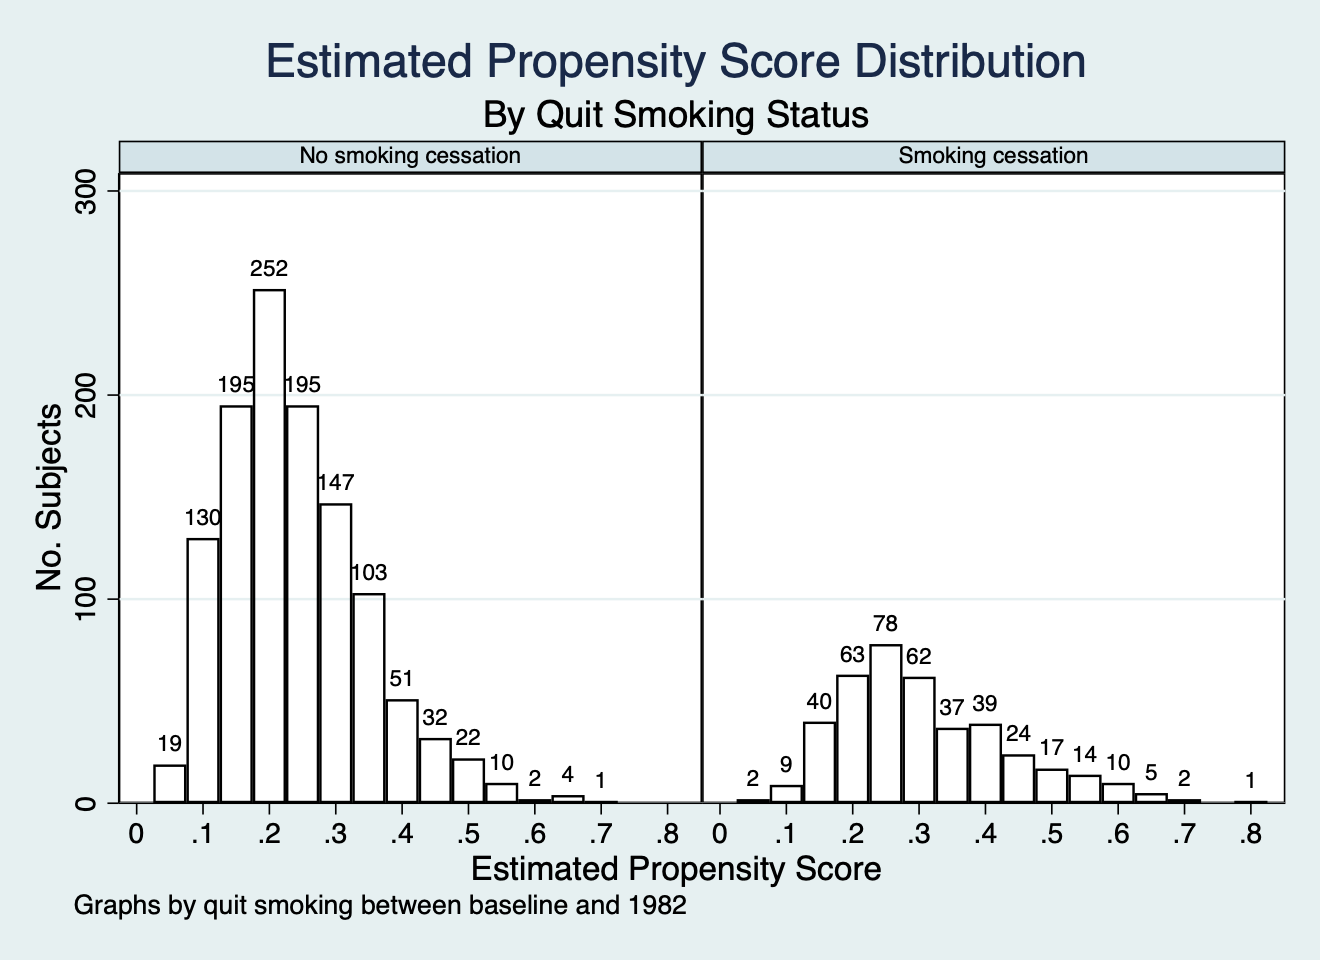
\includegraphics[width=0.85\linewidth]{./figs/stata-fig-15-2} \end{center}

\hypertarget{program-15.3-1}{%
\section{Program 15.3}\label{program-15.3-1}}

\begin{itemize}
\tightlist
\item
  Stratification and outcome regression using deciles of the propensity score
\item
  Data from NHEFS
\item
  Section 15.3
\item
  Note: Stata decides borderline cutpoints differently from SAS, so, despite identically distributed propensity scores, the results of regression using deciles are not an exact match with the book.
\end{itemize}

\begin{Shaded}
\begin{Highlighting}[]
\KeywordTok{use}\NormalTok{ ./}\KeywordTok{data}\NormalTok{/nhefs{-}ps, }\KeywordTok{clear}

\CommentTok{/*Calculation of deciles of ps*/}
\KeywordTok{xtile}\NormalTok{ ps\_dec = ps, nq(10)}
\KeywordTok{by}\NormalTok{ ps\_dec, }\KeywordTok{sort}\NormalTok{: }\KeywordTok{summarize}\NormalTok{ ps}

\CommentTok{/*Stratification on PS deciles, allowing for effect modification*/}
\CommentTok{/*Note: stata compares qsmk 0 vs qsmk 1, so the coefficients are reversed relative to the book*/}
\KeywordTok{by}\NormalTok{ ps\_dec: }\KeywordTok{ttest}\NormalTok{ wt82\_71, }\KeywordTok{by}\NormalTok{(qsmk)}

\CommentTok{/*Regression on PS deciles, with no product terms*/}
\KeywordTok{regress}\NormalTok{ wt82\_71 qsmk ib(}\FunctionTok{last}\NormalTok{).ps\_dec}
\end{Highlighting}
\end{Shaded}

\begin{verbatim}
-> ps_dec = 1

    Variable |        Obs        Mean    Std. dev.       Min        Max
-------------+---------------------------------------------------------
          ps |        157    .0976251    .0185215   .0510008   .1240482

--------------------------------------------------------------------------------
-> ps_dec = 2

    Variable |        Obs        Mean    Std. dev.       Min        Max
-------------+---------------------------------------------------------
          ps |        157    .1430792    .0107751   .1241923   .1603558

--------------------------------------------------------------------------------
-> ps_dec = 3

    Variable |        Obs        Mean    Std. dev.       Min        Max
-------------+---------------------------------------------------------
          ps |        156    .1750423     .008773   .1606041   .1893271

--------------------------------------------------------------------------------
-> ps_dec = 4

    Variable |        Obs        Mean    Std. dev.       Min        Max
-------------+---------------------------------------------------------
          ps |        157    .2014066    .0062403    .189365   .2121815

--------------------------------------------------------------------------------
-> ps_dec = 5

    Variable |        Obs        Mean    Std. dev.       Min        Max
-------------+---------------------------------------------------------
          ps |        156    .2245376    .0073655   .2123068    .237184

--------------------------------------------------------------------------------
-> ps_dec = 6

    Variable |        Obs        Mean    Std. dev.       Min        Max
-------------+---------------------------------------------------------
          ps |        157    .2515298    .0078777   .2377578   .2655718

--------------------------------------------------------------------------------
-> ps_dec = 7

    Variable |        Obs        Mean    Std. dev.       Min        Max
-------------+---------------------------------------------------------
          ps |        157    .2827476    .0099986   .2655724   .2994968

--------------------------------------------------------------------------------
-> ps_dec = 8

    Variable |        Obs        Mean    Std. dev.       Min        Max
-------------+---------------------------------------------------------
          ps |        156    .3204104    .0125102   .2997581   .3438773

--------------------------------------------------------------------------------
-> ps_dec = 9

    Variable |        Obs        Mean    Std. dev.       Min        Max
-------------+---------------------------------------------------------
          ps |        157     .375637    .0221347   .3439862   .4174631

--------------------------------------------------------------------------------
-> ps_dec = 10

    Variable |        Obs        Mean    Std. dev.       Min        Max
-------------+---------------------------------------------------------
          ps |        156    .5026508    .0733494   .4176717   .7768887



--------------------------------------------------------------------------------
-> ps_dec = 1

Two-sample t test with equal variances
------------------------------------------------------------------------------
   Group |     Obs        Mean    Std. err.   Std. dev.   [95% conf. interval]
---------+--------------------------------------------------------------------
No smoki |     146     3.74236    .6531341    7.891849    2.451467    5.033253
 Smoking |      11    3.949703    2.332995    7.737668   -1.248533     9.14794
---------+--------------------------------------------------------------------
Combined |     157    3.756887    .6270464    7.856869     2.51829    4.995484
---------+--------------------------------------------------------------------
    diff |           -.2073431    2.464411               -5.075509    4.660822
------------------------------------------------------------------------------
    diff = mean(No smoki) - mean(Smoking)                         t =  -0.0841
H0: diff = 0                                     Degrees of freedom =      155

    Ha: diff < 0                 Ha: diff != 0                 Ha: diff > 0
 Pr(T < t) = 0.4665         Pr(|T| > |t|) = 0.9331          Pr(T > t) = 0.5335

--------------------------------------------------------------------------------
-> ps_dec = 2

Two-sample t test with equal variances
------------------------------------------------------------------------------
   Group |     Obs        Mean    Std. err.   Std. dev.   [95% conf. interval]
---------+--------------------------------------------------------------------
No smoki |     134    2.813019     .589056    6.818816    1.647889    3.978149
 Smoking |      23    7.726944    1.260784    6.046508    5.112237    10.34165
---------+--------------------------------------------------------------------
Combined |     157    3.532893    .5519826    6.916322    2.442569    4.623217
---------+--------------------------------------------------------------------
    diff |           -4.913925    1.515494               -7.907613   -1.920237
------------------------------------------------------------------------------
    diff = mean(No smoki) - mean(Smoking)                         t =  -3.2425
H0: diff = 0                                     Degrees of freedom =      155

    Ha: diff < 0                 Ha: diff != 0                 Ha: diff > 0
 Pr(T < t) = 0.0007         Pr(|T| > |t|) = 0.0015          Pr(T > t) = 0.9993

--------------------------------------------------------------------------------
-> ps_dec = 3

Two-sample t test with equal variances
------------------------------------------------------------------------------
   Group |     Obs        Mean    Std. err.   Std. dev.   [95% conf. interval]
---------+--------------------------------------------------------------------
No smoki |     128     3.25684    .5334655    6.035473    2.201209    4.312472
 Smoking |      28    7.954974    1.418184    7.504324    5.045101    10.86485
---------+--------------------------------------------------------------------
Combined |     156    4.100095    .5245749    6.551938    3.063857    5.136334
---------+--------------------------------------------------------------------
    diff |           -4.698134    1.318074               -7.301973   -2.094294
------------------------------------------------------------------------------
    diff = mean(No smoki) - mean(Smoking)                         t =  -3.5644
H0: diff = 0                                     Degrees of freedom =      154

    Ha: diff < 0                 Ha: diff != 0                 Ha: diff > 0
 Pr(T < t) = 0.0002         Pr(|T| > |t|) = 0.0005          Pr(T > t) = 0.9998

--------------------------------------------------------------------------------
-> ps_dec = 4

Two-sample t test with equal variances
------------------------------------------------------------------------------
   Group |     Obs        Mean    Std. err.   Std. dev.   [95% conf. interval]
---------+--------------------------------------------------------------------
No smoki |     121    3.393929    .5267602    5.794362    2.350981    4.436877
 Smoking |      36    5.676072    1.543143    9.258861    2.543324    8.808819
---------+--------------------------------------------------------------------
Combined |     157    3.917223    .5412091     6.78133    2.848179    4.986266
---------+--------------------------------------------------------------------
    diff |           -2.282143    1.278494               -4.807663    .2433778
------------------------------------------------------------------------------
    diff = mean(No smoki) - mean(Smoking)                         t =  -1.7850
H0: diff = 0                                     Degrees of freedom =      155

    Ha: diff < 0                 Ha: diff != 0                 Ha: diff > 0
 Pr(T < t) = 0.0381         Pr(|T| > |t|) = 0.0762          Pr(T > t) = 0.9619

--------------------------------------------------------------------------------
-> ps_dec = 5

Two-sample t test with equal variances
------------------------------------------------------------------------------
   Group |     Obs        Mean    Std. err.   Std. dev.   [95% conf. interval]
---------+--------------------------------------------------------------------
No smoki |     119    1.368438    .8042619    8.773461   -.2242199    2.961095
 Smoking |      37    5.195421    1.388723     8.44727    2.378961    8.011881
---------+--------------------------------------------------------------------
Combined |     156     2.27612    .7063778    8.822656    .8807499    3.671489
---------+--------------------------------------------------------------------
    diff |           -3.826983    1.637279               -7.061407    -.592559
------------------------------------------------------------------------------
    diff = mean(No smoki) - mean(Smoking)                         t =  -2.3374
H0: diff = 0                                     Degrees of freedom =      154

    Ha: diff < 0                 Ha: diff != 0                 Ha: diff > 0
 Pr(T < t) = 0.0104         Pr(|T| > |t|) = 0.0207          Pr(T > t) = 0.9896

--------------------------------------------------------------------------------
-> ps_dec = 6

Two-sample t test with equal variances
------------------------------------------------------------------------------
   Group |     Obs        Mean    Std. err.   Std. dev.   [95% conf. interval]
---------+--------------------------------------------------------------------
No smoki |     112     2.25564    .6850004    7.249362    .8982664    3.613014
 Smoking |      45    7.199088    1.724899    11.57097    3.722782    10.67539
---------+--------------------------------------------------------------------
Combined |     157    3.672552    .7146582    8.954642    2.260897    5.084207
---------+--------------------------------------------------------------------
    diff |           -4.943447    1.535024               -7.975714   -1.911181
------------------------------------------------------------------------------
    diff = mean(No smoki) - mean(Smoking)                         t =  -3.2204
H0: diff = 0                                     Degrees of freedom =      155

    Ha: diff < 0                 Ha: diff != 0                 Ha: diff > 0
 Pr(T < t) = 0.0008         Pr(|T| > |t|) = 0.0016          Pr(T > t) = 0.9992

--------------------------------------------------------------------------------
-> ps_dec = 7

Two-sample t test with equal variances
------------------------------------------------------------------------------
   Group |     Obs        Mean    Std. err.   Std. dev.   [95% conf. interval]
---------+--------------------------------------------------------------------
No smoki |     116    .7948483    .7916172    8.525978    -.773193     2.36289
 Smoking |      41    6.646091     1.00182    6.414778    4.621337    8.670844
---------+--------------------------------------------------------------------
Combined |     157     2.32288    .6714693    8.413486    .9965349    3.649225
---------+--------------------------------------------------------------------
    diff |           -5.851242     1.45977               -8.734853   -2.967632
------------------------------------------------------------------------------
    diff = mean(No smoki) - mean(Smoking)                         t =  -4.0083
H0: diff = 0                                     Degrees of freedom =      155

    Ha: diff < 0                 Ha: diff != 0                 Ha: diff > 0
 Pr(T < t) = 0.0000         Pr(|T| > |t|) = 0.0001          Pr(T > t) = 1.0000

--------------------------------------------------------------------------------
-> ps_dec = 8

Two-sample t test with equal variances
------------------------------------------------------------------------------
   Group |     Obs        Mean    Std. err.   Std. dev.   [95% conf. interval]
---------+--------------------------------------------------------------------
No smoki |     107    1.063848    .5840159    6.041107   -.0940204    2.221716
 Smoking |      49    3.116263    1.113479    7.794356    .8774626    5.355063
---------+--------------------------------------------------------------------
Combined |     156    1.708517    .5352016    6.684666    .6512864    2.765747
---------+--------------------------------------------------------------------
    diff |           -2.052415    1.144914                -4.31418    .2093492
------------------------------------------------------------------------------
    diff = mean(No smoki) - mean(Smoking)                         t =  -1.7926
H0: diff = 0                                     Degrees of freedom =      154

    Ha: diff < 0                 Ha: diff != 0                 Ha: diff > 0
 Pr(T < t) = 0.0375         Pr(|T| > |t|) = 0.0750          Pr(T > t) = 0.9625

--------------------------------------------------------------------------------
-> ps_dec = 9

Two-sample t test with equal variances
------------------------------------------------------------------------------
   Group |     Obs        Mean    Std. err.   Std. dev.   [95% conf. interval]
---------+--------------------------------------------------------------------
No smoki |     100   -.0292906    .7637396    7.637396   -1.544716    1.486134
 Smoking |      57    .9112647    .9969309    7.526663   -1.085828    2.908357
---------+--------------------------------------------------------------------
Combined |     157    .3121849    .6054898    7.586766   -.8838316    1.508201
---------+--------------------------------------------------------------------
    diff |           -.9405554     1.26092                -3.43136    1.550249
------------------------------------------------------------------------------
    diff = mean(No smoki) - mean(Smoking)                         t =  -0.7459
H0: diff = 0                                     Degrees of freedom =      155

    Ha: diff < 0                 Ha: diff != 0                 Ha: diff > 0
 Pr(T < t) = 0.2284         Pr(|T| > |t|) = 0.4568          Pr(T > t) = 0.7716

--------------------------------------------------------------------------------
-> ps_dec = 10

Two-sample t test with equal variances
------------------------------------------------------------------------------
   Group |     Obs        Mean    Std. err.   Std. dev.   [95% conf. interval]
---------+--------------------------------------------------------------------
No smoki |      80    -.768504    .9224756    8.250872   -2.604646    1.067638
 Smoking |      76     2.39532    1.053132    9.180992    .2973737    4.493267
---------+--------------------------------------------------------------------
Combined |     156    .7728463    .7071067    8.831759   -.6239631    2.169656
---------+--------------------------------------------------------------------
    diff |           -3.163824    1.396178               -5.921957    -.405692
------------------------------------------------------------------------------
    diff = mean(No smoki) - mean(Smoking)                         t =  -2.2661
H0: diff = 0                                     Degrees of freedom =      154

    Ha: diff < 0                 Ha: diff != 0                 Ha: diff > 0
 Pr(T < t) = 0.0124         Pr(|T| > |t|) = 0.0248          Pr(T > t) = 0.9876

      Source |       SS           df       MS      Number of obs   =     1,566
-------------+----------------------------------   F(10, 1555)     =      9.87
       Model |   5799.7817        10   579.97817   Prob > F        =    0.0000
    Residual |  91375.8049     1,555  58.7625755   R-squared       =    0.0597
-------------+----------------------------------   Adj R-squared   =    0.0536
       Total |  97175.5866     1,565  62.0930266   Root MSE        =    7.6657

------------------------------------------------------------------------------
     wt82_71 | Coefficient  Std. err.      t    P>|t|     [95% conf. interval]
-------------+----------------------------------------------------------------
        qsmk |   3.356927   .4580399     7.33   0.000     2.458486    4.255368
             |
      ps_dec |
          1  |   4.384269   .8873947     4.94   0.000     2.643652    6.124885
          2  |   3.903694   .8805212     4.43   0.000      2.17656    5.630828
          3  |    4.36015   .8793345     4.96   0.000     2.635343    6.084956
          4  |   4.010061   .8745966     4.59   0.000     2.294548    5.725575
          5  |   2.342505   .8754878     2.68   0.008     .6252438    4.059766
          6  |   3.572955   .8714389     4.10   0.000     1.863636    5.282275
          7  |    2.30881   .8727462     2.65   0.008     .5969261    4.020693
          8  |   1.516677   .8715796     1.74   0.082    -.1929182    3.226273
          9  |  -.0439923   .8684465    -0.05   0.960    -1.747442    1.659457
             |
       _cons |  -.8625798   .6530529    -1.32   0.187    -2.143537    .4183773
------------------------------------------------------------------------------
\end{verbatim}

\hypertarget{program-15.4-1}{%
\section{Program 15.4}\label{program-15.4-1}}

\begin{itemize}
\tightlist
\item
  Standardization and outcome regression using the propensity score
\item
  Data from NHEFS
\item
  Section 15.3
\end{itemize}

\begin{Shaded}
\begin{Highlighting}[]
\KeywordTok{use}\NormalTok{ ./}\KeywordTok{data}\NormalTok{/nhefs{-}formatted, }\KeywordTok{clear}

\CommentTok{/*Estimate the propensity score*/}
\KeywordTok{logit}\NormalTok{ qsmk sex race c.age\#\#c.age ib(}\FunctionTok{last}\NormalTok{).education }\CommentTok{///}
\NormalTok{  c.smokeintensity\#\#c.smokeintensity }\CommentTok{///}
\NormalTok{  c.smokeyrs\#\#c.smokeyrs ib(}\FunctionTok{last}\NormalTok{).exercise }\CommentTok{///}
\NormalTok{  ib(}\FunctionTok{last}\NormalTok{).active c.wt71\#\#c.wt71 }
\KeywordTok{predict}\NormalTok{ ps, pr}

\CommentTok{/*Expand the dataset for standardization*/}
\NormalTok{expand 2, }\KeywordTok{generate}\NormalTok{(interv)}
\NormalTok{expand 2 }\KeywordTok{if}\NormalTok{ interv == 0, }\KeywordTok{generate}\NormalTok{(interv2)}
\KeywordTok{replace}\NormalTok{ interv = {-}1 }\KeywordTok{if}\NormalTok{ interv2 ==1}
\KeywordTok{drop}\NormalTok{ interv2 }
\KeywordTok{tab}\NormalTok{ interv}
\KeywordTok{replace}\NormalTok{ wt82\_71 = . }\KeywordTok{if}\NormalTok{ interv != {-}1}
\KeywordTok{replace}\NormalTok{ qsmk = 0 }\KeywordTok{if}\NormalTok{ interv == 0}
\KeywordTok{replace}\NormalTok{ qsmk = 1 }\KeywordTok{if}\NormalTok{ interv == 1}
\KeywordTok{by}\NormalTok{ interv, }\KeywordTok{sort}\NormalTok{: }\KeywordTok{summarize}\NormalTok{ qsmk}

\CommentTok{/*Regression on the propensity score, allowing for effect modification*/}
\KeywordTok{regress}\NormalTok{ wt82\_71 qsmk\#\#c.ps}
\KeywordTok{predict}\NormalTok{ predY, }\KeywordTok{xb}
\KeywordTok{by}\NormalTok{ interv, }\KeywordTok{sort}\NormalTok{: }\KeywordTok{summarize}\NormalTok{ predY}

\KeywordTok{quietly} \KeywordTok{summarize}\NormalTok{ predY }\KeywordTok{if}\NormalTok{(interv == {-}1)}
\FunctionTok{matrix}\NormalTok{ input observe = ({-}1,}\OtherTok{\textasciigrave{}r(mean)\textquotesingle{}}\NormalTok{)}
\KeywordTok{quietly} \KeywordTok{summarize}\NormalTok{ predY }\KeywordTok{if}\NormalTok{(interv == 0)}
\FunctionTok{matrix}\NormalTok{ observe = (observe \textbackslash{}0,}\OtherTok{\textasciigrave{}r(mean)\textquotesingle{}}\NormalTok{)}
\KeywordTok{quietly} \KeywordTok{summarize}\NormalTok{ predY }\KeywordTok{if}\NormalTok{(interv == 1)}
\FunctionTok{matrix}\NormalTok{ observe = (observe \textbackslash{}1,}\OtherTok{\textasciigrave{}r(mean)\textquotesingle{}}\NormalTok{)}
\FunctionTok{matrix}\NormalTok{ observe = (observe \textbackslash{}., observe[3,2]{-}observe[2,2]) }
\FunctionTok{matrix} \OtherTok{rownames}\NormalTok{ observe = observed E(Y(a=0)) E(Y(a=1)) difference}
\FunctionTok{matrix} \OtherTok{colnames}\NormalTok{ observe = interv }\OtherTok{value}
\FunctionTok{matrix} \OtherTok{list}\NormalTok{ observe }

\CommentTok{/*bootstrap program*/}
\KeywordTok{drop} \KeywordTok{if}\NormalTok{ interv != {-}1}
\KeywordTok{gen}\NormalTok{ meanY\_b =.}
\KeywordTok{qui} \KeywordTok{save}\NormalTok{ ./}\KeywordTok{data}\NormalTok{/nhefs\_std, }\KeywordTok{replace}

\KeywordTok{capture} \KeywordTok{program} \KeywordTok{drop}\NormalTok{ bootstdz}

\KeywordTok{program} \KeywordTok{define}\NormalTok{ bootstdz, rclass}
\KeywordTok{use}\NormalTok{ ./}\KeywordTok{data}\NormalTok{/nhefs\_std, }\KeywordTok{clear}
\KeywordTok{preserve}
\KeywordTok{bsample} 
\CommentTok{/*Create 2 new copies of the data. }
\CommentTok{Set the outcome AND the exposure to missing in the copies*/}
\NormalTok{expand 2, }\KeywordTok{generate}\NormalTok{(interv\_b)}
\NormalTok{expand 2 }\KeywordTok{if}\NormalTok{ interv\_b == 0, }\KeywordTok{generate}\NormalTok{(interv2\_b)}
\KeywordTok{qui} \KeywordTok{replace}\NormalTok{ interv\_b = {-}1 }\KeywordTok{if}\NormalTok{ interv2\_b ==1}
\KeywordTok{qui} \KeywordTok{drop}\NormalTok{ interv2\_b}
\KeywordTok{qui} \KeywordTok{replace}\NormalTok{ wt82\_71 = . }\KeywordTok{if}\NormalTok{ interv\_b != {-}1}
\KeywordTok{qui} \KeywordTok{replace}\NormalTok{ qsmk = . }\KeywordTok{if}\NormalTok{ interv\_b != {-}1}

\CommentTok{/*Fit the propensity score in the original data }
\CommentTok{(where qsmk is not missing) and generate predictions for everyone*/}
\KeywordTok{logit}\NormalTok{ qsmk sex race c.age\#\#c.age ib(}\FunctionTok{last}\NormalTok{).education }\CommentTok{///}
\NormalTok{  c.smokeintensity\#\#c.smokeintensity }\CommentTok{///}
\NormalTok{    c.smokeyrs\#\#c.smokeyrs ib(}\FunctionTok{last}\NormalTok{).exercise ib(}\FunctionTok{last}\NormalTok{).active }\CommentTok{///}
\NormalTok{    c.wt71\#\#c.wt71 }
\KeywordTok{predict}\NormalTok{ ps\_b, pr}

\CommentTok{/*Set the exposure to 0 for everyone in copy 0, }
\CommentTok{and 1 to everyone for copy 1*/}
\KeywordTok{qui} \KeywordTok{replace}\NormalTok{ qsmk = 0 }\KeywordTok{if}\NormalTok{ interv\_b == 0}
\KeywordTok{qui} \KeywordTok{replace}\NormalTok{ qsmk = 1 }\KeywordTok{if}\NormalTok{ interv\_b == 1}

\CommentTok{/*Fit the outcome regression in the original data }
\CommentTok{(where wt82\_71 is not missing) and }
\CommentTok{generate predictions for everyone*/}
\KeywordTok{regress}\NormalTok{ wt82\_71 qsmk\#\#c.ps}
\KeywordTok{predict}\NormalTok{ predY\_b, }\KeywordTok{xb}

\CommentTok{/*Summarize the predictions in each set of copies*/}
\KeywordTok{summarize}\NormalTok{ predY\_b }\KeywordTok{if}\NormalTok{ interv\_b == 0}
\FunctionTok{return} \FunctionTok{scalar}\NormalTok{ boot\_0 = }\FunctionTok{r}\NormalTok{(}\KeywordTok{mean}\NormalTok{)}
\KeywordTok{summarize}\NormalTok{ predY\_b }\KeywordTok{if}\NormalTok{ interv\_b == 1}
\FunctionTok{return} \FunctionTok{scalar}\NormalTok{ boot\_1 = }\FunctionTok{r}\NormalTok{(}\KeywordTok{mean}\NormalTok{)}
\FunctionTok{return} \FunctionTok{scalar}\NormalTok{ boot\_diff = }\FunctionTok{return}\NormalTok{(boot\_1) {-} }\FunctionTok{return}\NormalTok{(boot\_0)}
\KeywordTok{qui} \KeywordTok{drop}\NormalTok{ meanY\_b}
\KeywordTok{restore}
\KeywordTok{end}

\CommentTok{/*Then we use the \textasciigrave{}simulate\textasciigrave{} command to run the bootstraps }
\CommentTok{as many times as we want.}
\CommentTok{Start with reps(10) to make sure your code runs, }
\CommentTok{and then change to reps(1000) to generate your final CIs*/}
\KeywordTok{simulate}\NormalTok{ EY\_a0=}\FunctionTok{r}\NormalTok{(boot\_0) EY\_a1 = }\FunctionTok{r}\NormalTok{(boot\_1) }\CommentTok{///}
\NormalTok{  difference = }\FunctionTok{r}\NormalTok{(boot\_diff), reps(500) }\DecValTok{seed}\NormalTok{(1): bootstdz /}

\FunctionTok{matrix}\NormalTok{ pe = observe[2..4, 2]\textquotesingle{}}
\FunctionTok{matrix} \OtherTok{list}\NormalTok{ pe}
\KeywordTok{bstat}\NormalTok{, stat(pe) n(1629) }
\KeywordTok{estat} \KeywordTok{bootstrap}\NormalTok{, }\KeywordTok{p}
\end{Highlighting}
\end{Shaded}

\begin{verbatim}
Iteration 0:   log likelihood = -893.02712  
Iteration 1:   log likelihood = -839.70016  
Iteration 2:   log likelihood = -838.45045  
Iteration 3:   log likelihood = -838.44842  
Iteration 4:   log likelihood = -838.44842  

Logistic regression                                     Number of obs =  1,566
                                                        LR chi2(18)   = 109.16
                                                        Prob > chi2   = 0.0000
Log likelihood = -838.44842                             Pseudo R2     = 0.0611

-------------------------------------------------------------------------------
         qsmk | Coefficient  Std. err.      z    P>|z|     [95% conf. interval]
--------------+----------------------------------------------------------------
          sex |  -.5274782   .1540497    -3.42   0.001      -.82941   -.2255463
         race |  -.8392636   .2100668    -4.00   0.000    -1.250987   -.4275404
          age |   .1212052   .0512663     2.36   0.018     .0207251    .2216853
              |
  c.age#c.age |  -.0008246   .0005361    -1.54   0.124    -.0018753    .0002262
              |
    education |
           1  |  -.4759606   .2262238    -2.10   0.035    -.9193511   -.0325701
           2  |  -.5047361    .217597    -2.32   0.020    -.9312184   -.0782538
           3  |  -.3895288   .1914353    -2.03   0.042    -.7647351   -.0143226
           4  |  -.4123596   .2772868    -1.49   0.137    -.9558318    .1311126
              |
smokeintens~y |  -.0772704   .0152499    -5.07   0.000    -.1071596   -.0473812
              |
           c. |
smokeintens~y#|
           c. |
smokeintens~y |   .0010451   .0002866     3.65   0.000     .0004835    .0016068
              |
     smokeyrs |  -.0735966   .0277775    -2.65   0.008    -.1280395   -.0191538
              |
   c.smokeyrs#|
   c.smokeyrs |   .0008441   .0004632     1.82   0.068    -.0000637    .0017519
              |
     exercise |
           0  |   -.395704   .1872401    -2.11   0.035    -.7626878   -.0287201
           1  |  -.0408635   .1382674    -0.30   0.768    -.3118627    .2301357
              |
       active |
           0  |   -.176784   .2149721    -0.82   0.411    -.5981215    .2445535
           1  |  -.1448395   .2111472    -0.69   0.493    -.5586806    .2690015
              |
         wt71 |  -.0152357   .0263161    -0.58   0.563    -.0668144     .036343
              |
c.wt71#c.wt71 |   .0001352   .0001632     0.83   0.407    -.0001846     .000455
              |
        _cons |   -1.19407   1.398493    -0.85   0.393    -3.935066    1.546925
-------------------------------------------------------------------------------


(1,566 observations created)

(1,566 observations created)

(1,566 real changes made)



  Expanded observation |
                  type |      Freq.     Percent        Cum.
-----------------------+-----------------------------------
                    -1 |      1,566       33.33       33.33
  Original observation |      1,566       33.33       66.67
Duplicated observation |      1,566       33.33      100.00
-----------------------+-----------------------------------
                 Total |      4,698      100.00

(3,132 real changes made, 3,132 to missing)

(403 real changes made)

(1,163 real changes made)


--------------------------------------------------------------------------------
-> interv = -1

    Variable |        Obs        Mean    Std. dev.       Min        Max
-------------+---------------------------------------------------------
        qsmk |      1,566    .2573436    .4373099          0          1

--------------------------------------------------------------------------------
-> interv = Original

    Variable |        Obs        Mean    Std. dev.       Min        Max
-------------+---------------------------------------------------------
        qsmk |      1,566           0           0          0          0

--------------------------------------------------------------------------------
-> interv = Duplicat

    Variable |        Obs        Mean    Std. dev.       Min        Max
-------------+---------------------------------------------------------
        qsmk |      1,566           1           0          1          1

      Source |       SS           df       MS      Number of obs   =     1,566
-------------+----------------------------------   F(3, 1562)      =     29.96
       Model |  5287.31428         3  1762.43809   Prob > F        =    0.0000
    Residual |  91888.2723     1,562   58.827319   R-squared       =    0.0544
-------------+----------------------------------   Adj R-squared   =    0.0526
       Total |  97175.5866     1,565  62.0930266   Root MSE        =    7.6699

-------------------------------------------------------------------------------
      wt82_71 | Coefficient  Std. err.      t    P>|t|     [95% conf. interval]
--------------+----------------------------------------------------------------
         qsmk |
Smoking ce..  |   4.036457    1.13904     3.54   0.000      1.80225    6.270665
           ps |   -12.3319   2.129602    -5.79   0.000    -16.50908   -8.154716
              |
    qsmk#c.ps |
Smoking ce..  |  -2.038829   3.649684    -0.56   0.576    -9.197625    5.119967
              |
        _cons |   4.935432   .5570216     8.86   0.000     3.842843    6.028021
-------------------------------------------------------------------------------



--------------------------------------------------------------------------------
-> interv = -1

    Variable |        Obs        Mean    Std. dev.       Min        Max
-------------+---------------------------------------------------------
       predY |      1,566      2.6383    1.838063    -3.4687   8.111371

--------------------------------------------------------------------------------
-> interv = Original

    Variable |        Obs        Mean    Std. dev.       Min        Max
-------------+---------------------------------------------------------
       predY |      1,566    1.761898    1.433264  -4.645079   4.306496

--------------------------------------------------------------------------------
-> interv = Duplicat

    Variable |        Obs        Mean    Std. dev.       Min        Max
-------------+---------------------------------------------------------
       predY |      1,566    5.273676    1.670225  -2.192565   8.238971












observe[4,2]
               interv      value
  observed         -1  2.6382998
 E(Y(a=0))          0  1.7618979
 E(Y(a=1))          1  5.2736757
difference          .  3.5117778

(3,132 observations deleted)

(1,566 missing values generated)



 11. predict ps_b, pr
 12. 

      Command: bootstdz /
        EY_a0: r(boot_0)
        EY_a1: r(boot_1)
   difference: r(boot_diff)

Simulations (500)
----+--- 1 ---+--- 2 ---+--- 3 ---+--- 4 ---+--- 5 
..................................................    50
..................................................   100
..................................................   150
..................................................   200
..................................................   250
..................................................   300
..................................................   350
..................................................   400
..................................................   450
..................................................   500



pe[1,3]
        E(Y(a=0))   E(Y(a=1))  difference
value   1.7618979   5.2736757   3.5117778


Bootstrap results                                        Number of obs = 1,629
                                                         Replications  =   500

------------------------------------------------------------------------------
             |   Observed   Bootstrap                         Normal-based
             | coefficient  std. err.      z    P>|z|     [95% conf. interval]
-------------+----------------------------------------------------------------
       EY_a0 |   1.761898   .2255637     7.81   0.000     1.319801    2.203995
       EY_a1 |   5.273676   .4695378    11.23   0.000     4.353399    6.193953
  difference |   3.511778   .4970789     7.06   0.000     2.537521    4.486035
------------------------------------------------------------------------------


Bootstrap results                               Number of obs     =      1,629
                                                Replications      =        500

------------------------------------------------------------------------------
             |    Observed               Bootstrap
             | coefficient       Bias    std. err.  [95% conf. interval]
-------------+----------------------------------------------------------------
       EY_a0 |   1.7618979   .0026735   .22556365    1.269908   2.186845   (P)
       EY_a1 |   5.2736757  -.0049491   .46953779     4.34944   6.109205   (P)
  difference |   3.5117778  -.0076226   .49707894    2.466025   4.424034   (P)
------------------------------------------------------------------------------
Key: P: Percentile
\end{verbatim}

\hypertarget{instrumental-variables-estimation-stata}{%
\chapter*{16. Instrumental variables estimation: Stata}\label{instrumental-variables-estimation-stata}}
\addcontentsline{toc}{chapter}{16. Instrumental variables estimation: Stata}

\begin{Shaded}
\begin{Highlighting}[]
\FunctionTok{library}\NormalTok{(Statamarkdown)}
\end{Highlighting}
\end{Shaded}

\begin{verbatim}
/***************************************************************
Stata code for Causal Inference: What If by Miguel Hernan & Jamie Robins
Date: 10/10/2019
Author: Eleanor Murray 
For errors contact: ejmurray@bu.edu
***************************************************************/
\end{verbatim}

\hypertarget{program-16.1-1}{%
\section{Program 16.1}\label{program-16.1-1}}

\begin{itemize}
\tightlist
\item
  Estimating the average causal effect using the standard IV estimator via the calculation of sample averages
\item
  Data from NHEFS
\item
  Section 16.2
\end{itemize}

\begin{Shaded}
\begin{Highlighting}[]
\KeywordTok{use}\NormalTok{ ./}\KeywordTok{data}\NormalTok{/nhefs{-}formatted, }\KeywordTok{clear}

\KeywordTok{summarize}\NormalTok{ price82}

\CommentTok{/* ignore subjects with missing outcome or missing instrument for simplicity*/}
\KeywordTok{foreach} \KeywordTok{var} \KeywordTok{of} \KeywordTok{varlist}\NormalTok{ wt82 price82 \{}
  \KeywordTok{drop} \KeywordTok{if} \OtherTok{\textasciigrave{}var\textquotesingle{}}\NormalTok{==.}
\NormalTok{\}}

\CommentTok{/*Create categorical instrument*/}
\KeywordTok{gen} \KeywordTok{byte}\NormalTok{ highprice = (price82 \textgreater{} 1.5 \& price82 \textless{} .)}

\KeywordTok{save}\NormalTok{ ./}\KeywordTok{data}\NormalTok{/nhefs{-}highprice, }\KeywordTok{replace}

\CommentTok{/*Calculate P[Z|A=a]*/}
\KeywordTok{tab}\NormalTok{ highprice qsmk, }\OtherTok{row}

\CommentTok{/*Calculate P[Y|Z=z]*/}
\KeywordTok{ttest}\NormalTok{ wt82\_71, }\KeywordTok{by}\NormalTok{(highprice)}

\CommentTok{/*Final IV estimate, OPTION 1: Hand calculations*/}
\CommentTok{/*Numerator: num = E[Y|Z=1] {-} E[Y|Z=0] = 2.686 {-} 2.536 = 0.150*/}
\CommentTok{/*Denominator: denom = P[A=1|Z=1] {-} P[A=1|Z=0] = 0.258 {-} 0.195 = 0.063 */} 
\CommentTok{/*IV estimator: E[Ya=1] {-} E[Ya=0] = (E[Y|Z=1]{-}E[Y|Z=0])/(P[A=1|Z=1]{-}P[A=1|Z=0]) = 0.150/0.063 = 2.397*/}
\KeywordTok{display} \StringTok{"Numerator, E[Y|Z=1] {-} E[Y|Z=0] ="}\NormalTok{, 2.686 {-} 2.536}
\KeywordTok{display} \StringTok{"Denominator: denom = P[A=1|Z=1] {-} P[A=1|Z=0] ="}\NormalTok{, 0.258 {-} 0.195}
\KeywordTok{display} \StringTok{"IV estimator ="}\NormalTok{, 0.150/0.063}

\CommentTok{/*OPTION 2 2: automated calculation of instrument*/}
\CommentTok{/*Calculate P[A=1|Z=z], for each value of the instrument, }
\CommentTok{and store in a matrix*/}
\KeywordTok{quietly} \KeywordTok{summarize}\NormalTok{ qsmk }\KeywordTok{if}\NormalTok{ (highprice==0)}
\FunctionTok{matrix}\NormalTok{ input pa = (}\OtherTok{\textasciigrave{}r(mean)\textquotesingle{}}\NormalTok{)}
\KeywordTok{quietly} \KeywordTok{summarize}\NormalTok{ qsmk }\KeywordTok{if}\NormalTok{ (highprice==1)}
\FunctionTok{matrix}\NormalTok{ pa = (pa ,}\OtherTok{\textasciigrave{}r(mean)\textquotesingle{}}\NormalTok{)}
\FunctionTok{matrix} \OtherTok{list}\NormalTok{ pa}

\CommentTok{/*Calculate P[Y|Z=z], for each value of the instrument, }
\CommentTok{and store in a second matrix*/}
\KeywordTok{quietly} \KeywordTok{summarize}\NormalTok{ wt82\_71 }\KeywordTok{if}\NormalTok{ (highprice==0)}
\FunctionTok{matrix}\NormalTok{ input ey = (}\OtherTok{\textasciigrave{}r(mean)\textquotesingle{}}\NormalTok{)}
\KeywordTok{quietly} \KeywordTok{summarize}\NormalTok{ wt82\_71 }\KeywordTok{if}\NormalTok{ (highprice==1)}
\FunctionTok{matrix}\NormalTok{ ey = (ey ,}\OtherTok{\textasciigrave{}r(mean)\textquotesingle{}}\NormalTok{)}
\FunctionTok{matrix} \OtherTok{list}\NormalTok{ ey}

\CommentTok{/*Using Stata\textquotesingle{}s built{-}in matrix manipulation feature (Mata), }
\CommentTok{calculate numerator, denominator and IV estimator*/}
\NormalTok{*Numerator: num = E[Y|Z=1] {-} E[Y|Z=0]*}\KeywordTok{mata}
\NormalTok{*Denominator: denom = P[A=1|Z=1] {-} P[A=1|Z=0]*}
\NormalTok{*IV estimator: iv\_est = IV estimate }\KeywordTok{of}\NormalTok{ E[Ya=1] {-} E[Ya=0] *}
\KeywordTok{mata} 
\NormalTok{pa = st\_matrix(}\StringTok{"pa"}\NormalTok{)}
\NormalTok{ey = st\_matrix(}\StringTok{"ey"}\NormalTok{)}
\NormalTok{num = ey[1,2] {-} ey[1,1] }
\NormalTok{denom = pa[1,2] {-} pa[1,1]}
\NormalTok{iv\_est = num / denom }
\NormalTok{num}
\NormalTok{denom}
\NormalTok{st\_numscalar(}\StringTok{"iv\_est"}\NormalTok{, iv\_est)}
\KeywordTok{end}
\KeywordTok{di} \FunctionTok{scalar}\NormalTok{(iv\_est)}
\end{Highlighting}
\end{Shaded}

\begin{verbatim}
    Variable |        Obs        Mean    Std. dev.       Min        Max
-------------+---------------------------------------------------------
     price82 |      1,476    1.805989    .1301703   1.451904   2.103027

(0 observations deleted)
(90 observations deleted)


file ./data/nhefs-highprice.dta saved


+----------------+
| Key            |
|----------------|
|   frequency    |
| row percentage |
+----------------+

           | quit smoking between
           |   baseline and 1982
 highprice | No smokin  Smoking c |     Total
-----------+----------------------+----------
         0 |        33          8 |        41 
           |     80.49      19.51 |    100.00 
-----------+----------------------+----------
         1 |     1,065        370 |     1,435 
           |     74.22      25.78 |    100.00 
-----------+----------------------+----------
     Total |     1,098        378 |     1,476 
           |     74.39      25.61 |    100.00 


Two-sample t test with equal variances
------------------------------------------------------------------------------
   Group |     Obs        Mean    Std. err.   Std. dev.   [95% conf. interval]
---------+--------------------------------------------------------------------
       0 |      41    2.535729    1.461629    9.358993   -.4183336    5.489792
       1 |   1,435    2.686018    .2084888    7.897848    2.277042    3.094994
---------+--------------------------------------------------------------------
Combined |   1,476    2.681843    .2066282    7.938395    2.276527    3.087159
---------+--------------------------------------------------------------------
    diff |           -.1502887    1.257776               -2.617509    2.316932
------------------------------------------------------------------------------
    diff = mean(0) - mean(1)                                      t =  -0.1195
H0: diff = 0                                     Degrees of freedom =     1474

    Ha: diff < 0                 Ha: diff != 0                 Ha: diff > 0
 Pr(T < t) = 0.4525         Pr(|T| > |t|) = 0.9049          Pr(T > t) = 0.5475

Numerator, E[Y|Z=1] - E[Y|Z=0] = .15

Denominator: denom = P[A=1|Z=1] - P[A=1|Z=0] = .063

IV estimator = 2.3809524






pa[1,2]
           c1         c2
r1  .19512195  .25783972






ey[1,2]
           c1         c2
r1   2.535729  2.6860178

------------------------------------------------- mata (type end to exit) ------
: pa = st_matrix("pa")

: ey = st_matrix("ey")

: num = ey[1,2] - ey[1,1] 

: denom = pa[1,2] - pa[1,1]

: iv_est = num / denom 

: num
  .1502887173

: denom
  .06271777

: st_numscalar("iv_est", iv_est)

: end
--------------------------------------------------------------------------------

2.3962701
\end{verbatim}

\hypertarget{program-16.2-1}{%
\section{Program 16.2}\label{program-16.2-1}}

\begin{itemize}
\tightlist
\item
  Estimating the average causal effect using the standard IV estimator via two-stage-least-squares regression
\item
  Data from NHEFS
\item
  Section 16.2
\end{itemize}

\begin{Shaded}
\begin{Highlighting}[]
\KeywordTok{use}\NormalTok{ ./}\KeywordTok{data}\NormalTok{/nhefs{-}highprice, }\KeywordTok{clear}

\CommentTok{/* ivregress fits the model in two stages:}
\CommentTok{{-} first model: qsmk = highprice}
\CommentTok{{-} second model: wt82\_71 = predicted\_qsmk */}
\NormalTok{ivregress 2sls wt82\_71 (qsmk = highprice)}
\end{Highlighting}
\end{Shaded}

\begin{verbatim}
Instrumental variables 2SLS regression            Number of obs   =      1,476
                                                  Wald chi2(1)    =       0.01
                                                  Prob > chi2     =     0.9038
                                                  R-squared       =     0.0213
                                                  Root MSE        =     7.8508

------------------------------------------------------------------------------
     wt82_71 | Coefficient  Std. err.      z    P>|z|     [95% conf. interval]
-------------+----------------------------------------------------------------
        qsmk |    2.39627   19.82659     0.12   0.904    -36.46313    41.25567
       _cons |   2.068164   5.081652     0.41   0.684     -7.89169    12.02802
------------------------------------------------------------------------------
Instrumented: qsmk
 Instruments: highprice
\end{verbatim}

\hypertarget{program-16.3-1}{%
\section{Program 16.3}\label{program-16.3-1}}

\begin{itemize}
\tightlist
\item
  Estimating the average causal effect using the standard IV estimator via an additive marginal structural model
\item
  Data from NHEFS
\item
  Checking one possible value of psi.
\item
  See Chapter 14 for program that checks several values and computes 95\% confidence intervals\\
\item
  Section 16.2
\end{itemize}

\begin{Shaded}
\begin{Highlighting}[]
\KeywordTok{use}\NormalTok{ ./}\KeywordTok{data}\NormalTok{/nhefs{-}highprice, }\KeywordTok{clear}

\KeywordTok{gen}\NormalTok{ psi = 2.396}
\KeywordTok{gen}\NormalTok{ hspi = wt82\_71 {-} psi*qsmk}

\KeywordTok{logit}\NormalTok{ highprice hspi}
\end{Highlighting}
\end{Shaded}

\begin{verbatim}
Iteration 0:   log likelihood = -187.34948  
Iteration 1:   log likelihood = -187.34948  

Logistic regression                                     Number of obs =  1,476
                                                        LR chi2(1)    =   0.00
                                                        Prob > chi2   = 1.0000
Log likelihood = -187.34948                             Pseudo R2     = 0.0000

------------------------------------------------------------------------------
   highprice | Coefficient  Std. err.      z    P>|z|     [95% conf. interval]
-------------+----------------------------------------------------------------
        hspi |   2.75e-07   .0201749     0.00   1.000    -.0395419    .0395424
       _cons |   3.555347   .1637931    21.71   0.000     3.234319    3.876376
------------------------------------------------------------------------------
\end{verbatim}

\hypertarget{program-16.4-1}{%
\section{Program 16.4}\label{program-16.4-1}}

\begin{itemize}
\tightlist
\item
  Estimating the average causal effect using the standard IV estimator based on alternative proposed instruments
\item
  Data from NHEFS
\item
  Section 16.5
\end{itemize}

\begin{Shaded}
\begin{Highlighting}[]
\KeywordTok{use}\NormalTok{ ./}\KeywordTok{data}\NormalTok{/nhefs{-}highprice, }\KeywordTok{clear}

\CommentTok{/*Instrument cut{-}point: 1.6*/}
\KeywordTok{replace}\NormalTok{ highprice = .}
\KeywordTok{replace}\NormalTok{ highprice = (price82 \textgreater{}1.6 \& price82 \textless{} .)}

\NormalTok{ivregress 2sls wt82\_71 (qsmk = highprice)}

\CommentTok{/*Instrument cut{-}point: 1.7*/}
\KeywordTok{replace}\NormalTok{ highprice = .}
\KeywordTok{replace}\NormalTok{ highprice = (price82 \textgreater{}1.7 \& price82 \textless{} .)}

\NormalTok{ivregress 2sls wt82\_71 (qsmk = highprice)}

\CommentTok{/*Instrument cut{-}point: 1.8*/}
\KeywordTok{replace}\NormalTok{ highprice = .}
\KeywordTok{replace}\NormalTok{ highprice = (price82 \textgreater{}1.8 \& price82 \textless{} .)}

\NormalTok{ivregress 2sls wt82\_71 (qsmk = highprice)}

\CommentTok{/*Instrument cut{-}point: 1.9*/}
\KeywordTok{replace}\NormalTok{ highprice = .}
\KeywordTok{replace}\NormalTok{ highprice = (price82 \textgreater{}1.9 \& price82 \textless{} .)}

\NormalTok{ivregress 2sls wt82\_71 (qsmk = highprice)}
\end{Highlighting}
\end{Shaded}

\begin{verbatim}
(1,476 real changes made, 1,476 to missing)

(1,476 real changes made)


Instrumental variables 2SLS regression            Number of obs   =      1,476
                                                  Wald chi2(1)    =       0.06
                                                  Prob > chi2     =     0.8023
                                                  R-squared       =          .
                                                  Root MSE        =     18.593

------------------------------------------------------------------------------
     wt82_71 | Coefficient  Std. err.      z    P>|z|     [95% conf. interval]
-------------+----------------------------------------------------------------
        qsmk |   41.28124   164.8417     0.25   0.802    -281.8026     364.365
       _cons |  -7.890182   42.21833    -0.19   0.852    -90.63659    74.85623
------------------------------------------------------------------------------
Instrumented: qsmk
 Instruments: highprice

(1,476 real changes made, 1,476 to missing)

(1,476 real changes made)


Instrumental variables 2SLS regression            Number of obs   =      1,476
                                                  Wald chi2(1)    =       0.05
                                                  Prob > chi2     =     0.8274
                                                  R-squared       =          .
                                                  Root MSE        =     20.577

------------------------------------------------------------------------------
     wt82_71 | Coefficient  Std. err.      z    P>|z|     [95% conf. interval]
-------------+----------------------------------------------------------------
        qsmk |  -40.91185   187.6162    -0.22   0.827    -408.6328    326.8091
       _cons |   13.15927   48.05103     0.27   0.784    -81.01901    107.3375
------------------------------------------------------------------------------
Instrumented: qsmk
 Instruments: highprice

(1,476 real changes made, 1,476 to missing)

(1,476 real changes made)


Instrumental variables 2SLS regression            Number of obs   =      1,476
                                                  Wald chi2(1)    =       0.55
                                                  Prob > chi2     =     0.4576
                                                  R-squared       =          .
                                                  Root MSE        =      13.01

------------------------------------------------------------------------------
     wt82_71 | Coefficient  Std. err.      z    P>|z|     [95% conf. interval]
-------------+----------------------------------------------------------------
        qsmk |  -21.10342   28.40885    -0.74   0.458    -76.78374    34.57691
       _cons |   8.086377   7.283314     1.11   0.267    -6.188657    22.36141
------------------------------------------------------------------------------
Instrumented: qsmk
 Instruments: highprice

(1,476 real changes made, 1,476 to missing)

(1,476 real changes made)


Instrumental variables 2SLS regression            Number of obs   =      1,476
                                                  Wald chi2(1)    =       0.29
                                                  Prob > chi2     =     0.5880
                                                  R-squared       =          .
                                                  Root MSE        =     10.357

------------------------------------------------------------------------------
     wt82_71 | Coefficient  Std. err.      z    P>|z|     [95% conf. interval]
-------------+----------------------------------------------------------------
        qsmk |  -12.81141   23.65099    -0.54   0.588    -59.16649    33.54368
       _cons |   5.962813   6.062956     0.98   0.325    -5.920362    17.84599
------------------------------------------------------------------------------
Instrumented: qsmk
 Instruments: highprice
\end{verbatim}

\hypertarget{program-16.5-1}{%
\section{Program 16.5}\label{program-16.5-1}}

\begin{itemize}
\tightlist
\item
  Estimating the average causal effect using the standard IV estimator conditional on baseline covariates
\item
  Data from NHEFS
\item
  Section 16.5
\end{itemize}

\begin{Shaded}
\begin{Highlighting}[]
\KeywordTok{use}\NormalTok{ ./}\KeywordTok{data}\NormalTok{/nhefs{-}highprice, }\KeywordTok{clear}

\KeywordTok{replace}\NormalTok{ highprice = .}
\KeywordTok{replace}\NormalTok{ highprice = (price82 \textgreater{}1.5 \& price82 \textless{} .)}

\NormalTok{ivregress 2sls wt82\_71 sex race c.age c.smokeintensity }\CommentTok{///}
\NormalTok{  c.smokeyrs i.exercise i.active c.wt7 }\CommentTok{///}
\NormalTok{  (qsmk = highprice)}
\end{Highlighting}
\end{Shaded}

\begin{verbatim}
(1,476 real changes made, 1,476 to missing)

(1,476 real changes made)


Instrumental variables 2SLS regression            Number of obs   =      1,476
                                                  Wald chi2(11)   =     135.18
                                                  Prob > chi2     =     0.0000
                                                  R-squared       =     0.0622
                                                  Root MSE        =     7.6848

-------------------------------------------------------------------------------
      wt82_71 | Coefficient  Std. err.      z    P>|z|     [95% conf. interval]
--------------+----------------------------------------------------------------
         qsmk |  -1.042295   29.86522    -0.03   0.972    -59.57705    57.49246
          sex |  -1.644393   2.620115    -0.63   0.530    -6.779724    3.490938
         race |  -.1832546   4.631443    -0.04   0.968    -9.260716    8.894207
          age |    -.16364   .2395678    -0.68   0.495    -.6331844    .3059043
smokeintens~y |   .0057669    .144911     0.04   0.968    -.2782534    .2897872
     smokeyrs |   .0258357   .1607639     0.16   0.872    -.2892558    .3409271
              |
     exercise |
           1  |   .4987479   2.162395     0.23   0.818    -3.739469    4.736964
           2  |   .5818337   2.174255     0.27   0.789    -3.679628    4.843296
              |
       active |
           1  |  -1.170145   .6049921    -1.93   0.053    -2.355908    .0156176
           2  |  -.5122842   1.303121    -0.39   0.694    -3.066355    2.041787
              |
         wt71 |  -.0979493    .036123    -2.71   0.007     -.168749   -.0271496
        _cons |   17.28033    2.32589     7.43   0.000     12.72167    21.83899
-------------------------------------------------------------------------------
Instrumented: qsmk
 Instruments: sex race age smokeintensity smokeyrs 1.exercise 2.exercise
              1.active 2.active wt71 highprice
\end{verbatim}

\hypertarget{causal-survival-analysis-stata}{%
\chapter*{17. Causal survival analysis: Stata}\label{causal-survival-analysis-stata}}
\addcontentsline{toc}{chapter}{17. Causal survival analysis: Stata}

\begin{Shaded}
\begin{Highlighting}[]
\FunctionTok{library}\NormalTok{(Statamarkdown)}
\end{Highlighting}
\end{Shaded}

\begin{verbatim}
/***************************************************************
Stata code for Causal Inference: What If by Miguel Hernan & Jamie Robins
Date: 10/10/2019
Author: Eleanor Murray 
For errors contact: ejmurray@bu.edu
***************************************************************/
\end{verbatim}

\hypertarget{program-17.1-1}{%
\section{Program 17.1}\label{program-17.1-1}}

\begin{itemize}
\tightlist
\item
  Nonparametric estimation of survival curves
\item
  Data from NHEFS
\item
  Section 17.1
\end{itemize}

\begin{Shaded}
\begin{Highlighting}[]
\KeywordTok{use}\NormalTok{ ./}\KeywordTok{data}\NormalTok{/nhefs{-}formatted, }\KeywordTok{clear}

\CommentTok{/*Some preprocessing of the data*/}
\KeywordTok{gen}\NormalTok{ survtime = .}
\KeywordTok{replace}\NormalTok{ survtime = 120 }\KeywordTok{if}\NormalTok{ death == 0}
\KeywordTok{replace}\NormalTok{ survtime = (yrdth {-} 83)*12 + modth }\KeywordTok{if}\NormalTok{ death ==1}
\NormalTok{* yrdth ranges from 83 to 92*}

\KeywordTok{tab}\NormalTok{ death qsmk}

\CommentTok{/*Kaplan{-}Meier graph of observed survival over time, by quitting smoking*/}
\NormalTok{*For now, we }\KeywordTok{use}\NormalTok{ the }\KeywordTok{stset} \KeywordTok{function} \KeywordTok{in}\NormalTok{ Stata*}
\KeywordTok{stset}\NormalTok{ survtime, failure(death=1)}
\KeywordTok{sts} \KeywordTok{graph}\NormalTok{, }\KeywordTok{by}\NormalTok{(qsmk) }\KeywordTok{xlabel}\NormalTok{(0(12)120)}
\KeywordTok{qui} \KeywordTok{gr} \KeywordTok{export}\NormalTok{ ./figs/stata{-}fig{-}17{-}1.png, }\KeywordTok{replace}
\end{Highlighting}
\end{Shaded}

\begin{verbatim}
(1,566 missing values generated)

(1,275 real changes made)

(291 real changes made)

     death |
   between | quit smoking between
  1983 and |   baseline and 1982
      1992 | No smokin  Smoking c |     Total
-----------+----------------------+----------
         0 |       963        312 |     1,275 
         1 |       200         91 |       291 
-----------+----------------------+----------
     Total |     1,163        403 |     1,566 


Survival-time data settings

         Failure event: death==1
Observed time interval: (0, survtime]
     Exit on or before: failure

--------------------------------------------------------------------------
      1,566  total observations
          0  exclusions
--------------------------------------------------------------------------
      1,566  observations remaining, representing
        291  failures in single-record/single-failure data
    171,076  total analysis time at risk and under observation
                                                At risk from t =         0
                                     Earliest observed entry t =         0
                                          Last observed exit t =       120

        Failure _d: death==1
  Analysis time _t: survtime
\end{verbatim}

\begin{center}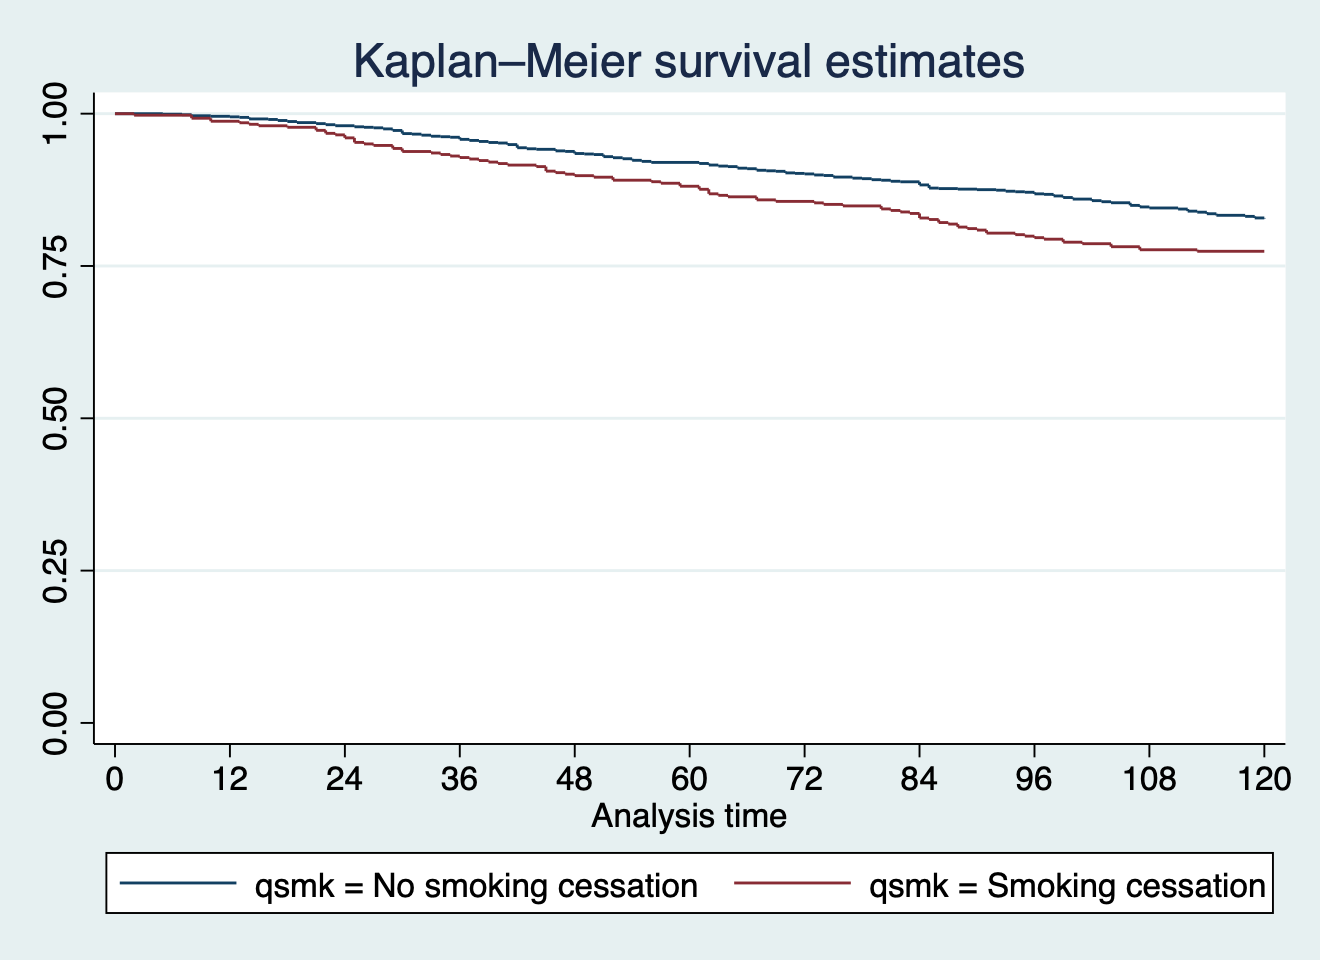
\includegraphics[width=0.85\linewidth]{./figs/stata-fig-17-1} \end{center}

\hypertarget{program-17.2-1}{%
\section{Program 17.2}\label{program-17.2-1}}

\begin{itemize}
\tightlist
\item
  Parametric estimation of survival curves via hazards model
\item
  Data from NHEFS
\item
  Section 17.1
\item
  Generates Figure 17.4
\end{itemize}

\begin{Shaded}
\begin{Highlighting}[]
\CommentTok{/**Create person{-}month dataset for survival analyses**/}

\CommentTok{/* We want our new dataset to include 1 observation per person }
\CommentTok{per month alive, starting at time = 0.}
\CommentTok{Individuals who survive to the end of follow{-}up will have }
\CommentTok{119 time points}
\CommentTok{Individuals who die will have survtime {-} 1 time points*/}

\KeywordTok{use}\NormalTok{ ./}\KeywordTok{data}\NormalTok{/nhefs{-}formatted, }\KeywordTok{clear}

\KeywordTok{gen}\NormalTok{ survtime = .}
\KeywordTok{replace}\NormalTok{ survtime = 120 }\KeywordTok{if}\NormalTok{ death == 0}
\KeywordTok{replace}\NormalTok{ survtime = (yrdth {-} 83)*12 + modth }\KeywordTok{if}\NormalTok{ death ==1}

\NormalTok{*expand }\KeywordTok{data}\NormalTok{ to person{-}time*}
\KeywordTok{gen}\NormalTok{ time = 0}
\NormalTok{expand survtime }\KeywordTok{if}\NormalTok{ time == 0}
\KeywordTok{bysort}\NormalTok{ seqn: }\KeywordTok{replace}\NormalTok{ time = }\DataTypeTok{\_n}\NormalTok{ {-} 1}

\NormalTok{*Create event }\KeywordTok{variable}\NormalTok{*}
\KeywordTok{gen}\NormalTok{ event = 0}
\KeywordTok{replace}\NormalTok{ event = 1 }\KeywordTok{if}\NormalTok{ time == survtime {-} 1 \& death == 1}
\KeywordTok{tab}\NormalTok{ event}

\NormalTok{*Create time{-}squared }\KeywordTok{variable} \KeywordTok{for}\NormalTok{ analyses*}
\KeywordTok{gen}\NormalTok{ timesq = time*time}

\NormalTok{*Save the dataset to your working directory }\KeywordTok{for}\NormalTok{ future }\KeywordTok{use}\NormalTok{*}
\KeywordTok{qui} \KeywordTok{save}\NormalTok{ ./}\KeywordTok{data}\NormalTok{/nhefs\_surv, }\KeywordTok{replace}

\CommentTok{/**Hazard ratios**/}
\KeywordTok{use}\NormalTok{ ./}\KeywordTok{data}\NormalTok{/nhefs\_surv, }\KeywordTok{clear}

\NormalTok{*Fit a pooled }\KeywordTok{logistic}\NormalTok{ hazards }\KeywordTok{model}\NormalTok{ *}
\KeywordTok{logistic}\NormalTok{ event qsmk qsmk\#c.time qsmk\#c.time\#c.time }\CommentTok{///}
\NormalTok{  c.time c.time\#c.time }

\CommentTok{/**Survival curves: run regression then do:**/}

\NormalTok{*Create a dataset with }\OtherTok{all}\NormalTok{ time points under each treatment }\DecValTok{level}\NormalTok{*}
\NormalTok{*Re{-}expand }\KeywordTok{data}\NormalTok{ with }\BaseNTok{rows} \KeywordTok{for} \OtherTok{all}\NormalTok{ timepoints*}
\KeywordTok{drop} \KeywordTok{if}\NormalTok{ time != 0}
\NormalTok{expand 120 }\KeywordTok{if}\NormalTok{ time ==0 }
\KeywordTok{bysort}\NormalTok{ seqn: }\KeywordTok{replace}\NormalTok{ time = }\DataTypeTok{\_n}\NormalTok{ {-} 1   }
        
\CommentTok{/*Create 2 copies of each subject, and set outcome to missing }
\CommentTok{and treatment {-}{-} use only the newobs*/}
\NormalTok{expand 2 , }\KeywordTok{generate}\NormalTok{(interv) }
\KeywordTok{replace}\NormalTok{ qsmk = interv   }

\CommentTok{/*Generate predicted event and survival probabilities }
\CommentTok{for each person each month in copies*/}
\KeywordTok{predict}\NormalTok{ pevent\_k, pr}
\KeywordTok{gen}\NormalTok{ psurv\_k = 1{-}pevent\_k}
\KeywordTok{keep}\NormalTok{ seqn time qsmk interv psurv\_k }

\NormalTok{*Within copies, }\KeywordTok{generate}\NormalTok{ predicted survival }\BaseNTok{over}\NormalTok{ time*}
\NormalTok{*Remember, survival is the product }\KeywordTok{of}\NormalTok{ conditional survival probabilities }\KeywordTok{in}\NormalTok{ each interval*  }
\KeywordTok{sort}\NormalTok{ seqn interv time}
\KeywordTok{gen}\NormalTok{ \_t = time + 1}
\KeywordTok{gen}\NormalTok{ psurv = psurv\_k }\KeywordTok{if}\NormalTok{ \_t ==1       }
\KeywordTok{bysort}\NormalTok{ seqn interv: }\KeywordTok{replace}\NormalTok{ psurv = psurv\_k*psurv[\_t{-}1] }\KeywordTok{if}\NormalTok{ \_t \textgreater{}1 }

\NormalTok{*Display 10{-}}\FunctionTok{year}\NormalTok{ standardized survival, under interventions*}
\NormalTok{*Note: since time starts }\FunctionTok{at}\NormalTok{ 0, }\FunctionTok{month}\NormalTok{ 119 is 10{-}}\FunctionTok{year}\NormalTok{ survival*}
\KeywordTok{by}\NormalTok{ interv, }\KeywordTok{sort}\NormalTok{: }\KeywordTok{summarize}\NormalTok{ psurv }\KeywordTok{if}\NormalTok{ time == 119}

\NormalTok{*Graph }\KeywordTok{of}\NormalTok{ standardized survival }\BaseNTok{over}\NormalTok{ time, under interventions*}
\CommentTok{/*Note, we want our graph to start at 100\% survival, }
\CommentTok{so add an extra time point with P(surv) = 1*/}
\NormalTok{expand 2 }\KeywordTok{if}\NormalTok{ time ==0, }\KeywordTok{generate}\NormalTok{(newtime)}
\KeywordTok{replace}\NormalTok{ psurv  = 1 }\KeywordTok{if}\NormalTok{ newtime == 1}
\KeywordTok{gen}\NormalTok{ time2 = 0 }\KeywordTok{if}\NormalTok{ newtime ==1}
\KeywordTok{replace}\NormalTok{ time2 = time + 1 }\KeywordTok{if}\NormalTok{ newtime == 0}

\CommentTok{/*Separate the survival probabilities to allow plotting by }
\CommentTok{intervention on qsmk*/}
\KeywordTok{separate}\NormalTok{ psurv, }\KeywordTok{by}\NormalTok{(interv)}

\NormalTok{*Plot the curves*}
\KeywordTok{twoway}\NormalTok{ (}\KeywordTok{line}\NormalTok{ psurv0 time2, }\KeywordTok{sort}\NormalTok{) }\CommentTok{///}
\NormalTok{  (}\KeywordTok{line}\NormalTok{ psurv1 time2, }\KeywordTok{sort}\NormalTok{) }\KeywordTok{if}\NormalTok{ interv \textgreater{} {-}1 }\CommentTok{///}
\NormalTok{  , }\KeywordTok{ylabel}\NormalTok{(0.5(0.1)1.0) }\KeywordTok{xlabel}\NormalTok{(0(12)120) }\CommentTok{///}
  \BaseNTok{ytitle}\NormalTok{(}\StringTok{"Survival probability"}\NormalTok{) }\BaseNTok{xtitle}\NormalTok{(}\StringTok{"Months of follow{-}up"}\NormalTok{) }\CommentTok{///}
  \BaseNTok{legend}\NormalTok{(}\KeywordTok{label}\NormalTok{(1 }\StringTok{"A=0"}\NormalTok{) }\KeywordTok{label}\NormalTok{(2 }\StringTok{"A=1"}\NormalTok{))}
\KeywordTok{qui} \KeywordTok{gr} \KeywordTok{export}\NormalTok{ ./figs/stata{-}fig{-}17{-}2.png, }\KeywordTok{replace}
\end{Highlighting}
\end{Shaded}

\begin{verbatim}
(1,566 missing values generated)

(1,275 real changes made)

(291 real changes made)


(169,510 observations created)

(169510 real changes made)


(291 real changes made)

      event |      Freq.     Percent        Cum.
------------+-----------------------------------
          0 |    170,785       99.83       99.83
          1 |        291        0.17      100.00
------------+-----------------------------------
      Total |    171,076      100.00





Logistic regression                                    Number of obs = 171,076
                                                       LR chi2(5)    =   24.26
                                                       Prob > chi2   =  0.0002
Log likelihood = -2134.1973                            Pseudo R2     =  0.0057

-------------------------------------------------------------------------------
        event | Odds ratio   Std. err.      z    P>|z|     [95% conf. interval]
--------------+----------------------------------------------------------------
         qsmk |   1.402527   .6000025     0.79   0.429     .6064099    3.243815
              |
  qsmk#c.time |
Smoking ce..  |   1.012318   .0162153     0.76   0.445     .9810299    1.044603
              |
  qsmk#c.time#|
       c.time |
Smoking ce..  |   .9998342   .0001321    -1.25   0.210     .9995753    1.000093
              |
         time |   1.022048   .0090651     2.46   0.014     1.004434    1.039971
              |
c.time#c.time |   .9998637   .0000699    -1.95   0.051     .9997266    1.000001
              |
        _cons |   .0007992   .0001972   -28.90   0.000     .0004927    .0012963
-------------------------------------------------------------------------------
Note: _cons estimates baseline odds.

(169,510 observations deleted)

(186,354 observations created)

(186354 real changes made)

(187,920 observations created)

(187,920 real changes made)






(372,708 missing values generated)

(372708 real changes made)


--------------------------------------------------------------------------------
-> interv = Original

    Variable |        Obs        Mean    Std. dev.       Min        Max
-------------+---------------------------------------------------------
       psurv |      1,566    .8279829           0   .8279829   .8279829

--------------------------------------------------------------------------------
-> interv = Duplicat

    Variable |        Obs        Mean    Std. dev.       Min        Max
-------------+---------------------------------------------------------
       psurv |      1,566     .774282           0    .774282    .774282


(3,132 observations created)

(3,132 real changes made)

(375,840 missing values generated)

(375,840 real changes made)


Variable      Storage   Display    Value
    name         type    format    label      Variable label
--------------------------------------------------------------------------------
psurv0          float   %9.0g                 psurv, interv == Original
                                                observation
psurv1          float   %9.0g                 psurv, interv == Duplicated
                                                observation
\end{verbatim}

\begin{center}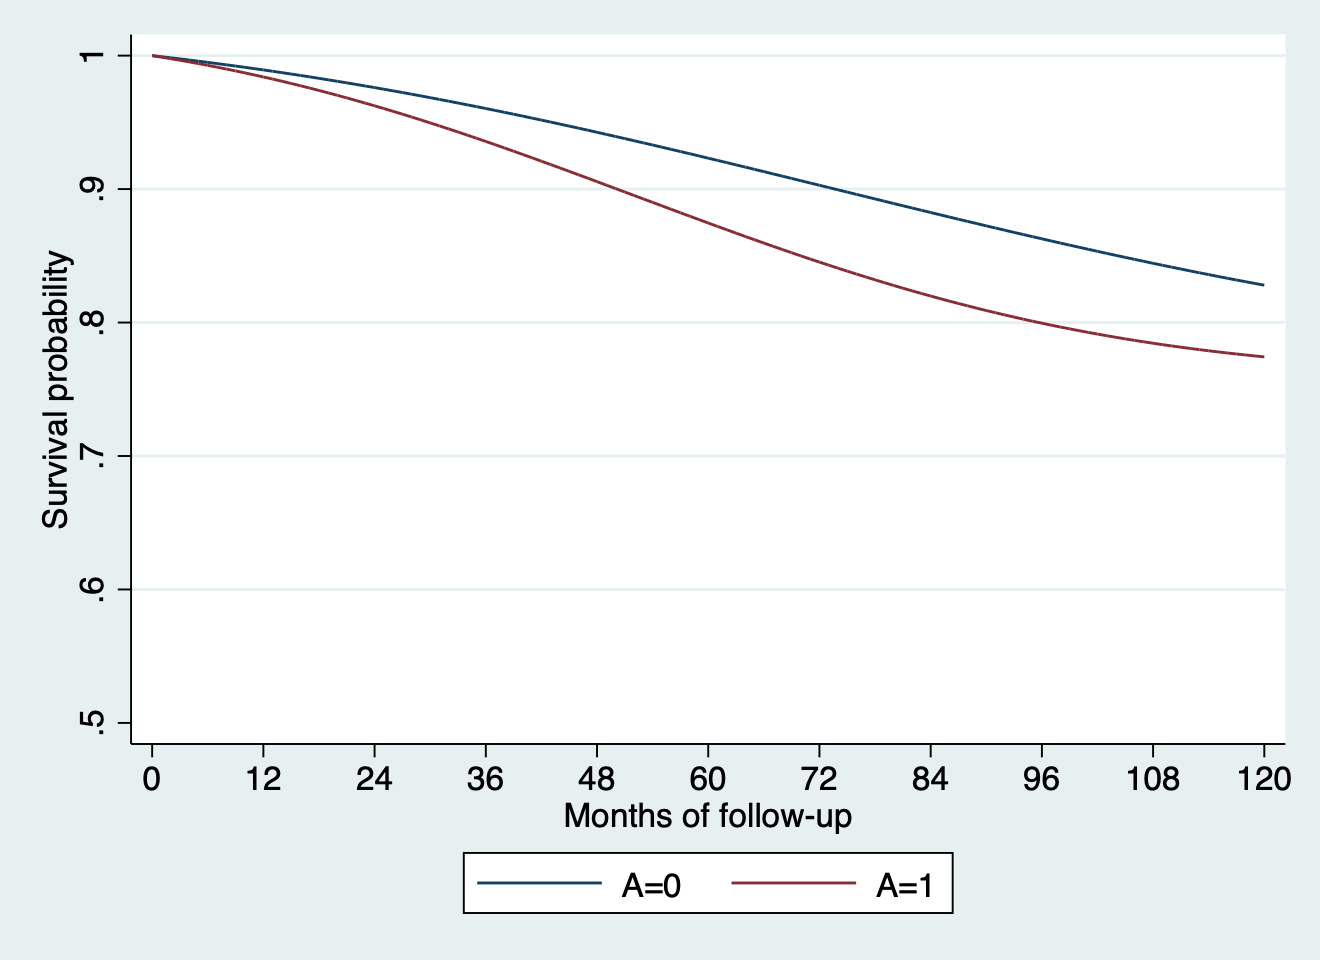
\includegraphics[width=0.85\linewidth]{./figs/stata-fig-17-2} \end{center}

\hypertarget{program-17.3-1}{%
\section{Program 17.3}\label{program-17.3-1}}

\begin{itemize}
\tightlist
\item
  Estimation of survival curves via IP weighted hazards model
\item
  Data from NHEFS
\item
  Section 17.4
\item
  Generates Figure 17.6
\end{itemize}

\begin{Shaded}
\begin{Highlighting}[]
\KeywordTok{use}\NormalTok{ ./}\KeywordTok{data}\NormalTok{/nhefs\_surv, }\KeywordTok{clear}

\KeywordTok{keep}\NormalTok{ seqn event qsmk time sex race age education }\CommentTok{///}
\NormalTok{  smokeintensity smkintensity82\_71 smokeyrs }\CommentTok{///}
\NormalTok{  exercise active wt71}
\KeywordTok{preserve} 

\NormalTok{*Estimate weights*}
\KeywordTok{logit}\NormalTok{ qsmk sex race c.age\#\#c.age ib(}\FunctionTok{last}\NormalTok{).education }\CommentTok{///}
\NormalTok{  c.smokeintensity\#\#c.smokeintensity }\CommentTok{///}
\NormalTok{  c.smokeyrs\#\#c.smokeyrs ib(}\FunctionTok{last}\NormalTok{).exercise }\CommentTok{///}
\NormalTok{  ib(}\FunctionTok{last}\NormalTok{).active c.wt71\#\#c.wt71 }\KeywordTok{if}\NormalTok{ time == 0}
\KeywordTok{predict}\NormalTok{ p\_qsmk, pr}

\KeywordTok{logit}\NormalTok{ qsmk }\KeywordTok{if}\NormalTok{ time ==0 }
\KeywordTok{predict}\NormalTok{ num, pr}
\KeywordTok{gen} \KeywordTok{sw}\NormalTok{=num/p\_qsmk }\KeywordTok{if}\NormalTok{ qsmk==1}
\KeywordTok{replace} \KeywordTok{sw}\NormalTok{=(1{-}num)/(1{-}p\_qsmk) }\KeywordTok{if}\NormalTok{ qsmk==0}
\KeywordTok{summarize} \KeywordTok{sw}

\NormalTok{*IP weighted survival }\KeywordTok{by}\NormalTok{ smoking cessation*}
\KeywordTok{logit}\NormalTok{ event qsmk qsmk\#c.time qsmk\#c.time\#c.time }\CommentTok{///}
\NormalTok{  c.time c.time\#c.time [}\KeywordTok{pweight}\NormalTok{=}\KeywordTok{sw}\NormalTok{] , }\KeywordTok{cluster}\NormalTok{(seqn) }

\NormalTok{*Create a dataset with }\OtherTok{all}\NormalTok{ time points under each treatment }\DecValTok{level}\NormalTok{*}
\NormalTok{*Re{-}expand }\KeywordTok{data}\NormalTok{ with }\BaseNTok{rows} \KeywordTok{for} \OtherTok{all}\NormalTok{ timepoints*}
\KeywordTok{drop} \KeywordTok{if}\NormalTok{ time != 0}
\NormalTok{expand 120 }\KeywordTok{if}\NormalTok{ time ==0 }
\KeywordTok{bysort}\NormalTok{ seqn: }\KeywordTok{replace}\NormalTok{ time = }\DataTypeTok{\_n}\NormalTok{ {-} 1       }
        
\CommentTok{/*Create 2 copies of each subject, and set outcome }
\CommentTok{to missing and treatment {-}{-} use only the newobs*/}
\NormalTok{expand 2 , }\KeywordTok{generate}\NormalTok{(interv) }
\KeywordTok{replace}\NormalTok{ qsmk = interv   }

\CommentTok{/*Generate predicted event and survival probabilities }
\CommentTok{for each person each month in copies*/}
\KeywordTok{predict}\NormalTok{ pevent\_k, pr}
\KeywordTok{gen}\NormalTok{ psurv\_k = 1{-}pevent\_k}
\KeywordTok{keep}\NormalTok{ seqn time qsmk interv psurv\_k }

\NormalTok{*Within copies, }\KeywordTok{generate}\NormalTok{ predicted survival }\BaseNTok{over}\NormalTok{ time*}
\CommentTok{/*Remember, survival is the product of conditional survival}
\CommentTok{probabilities in each interval*/}
\KeywordTok{sort}\NormalTok{ seqn interv time}
\KeywordTok{gen}\NormalTok{ \_t = time + 1}
\KeywordTok{gen}\NormalTok{ psurv = psurv\_k }\KeywordTok{if}\NormalTok{ \_t ==1       }
\KeywordTok{bysort}\NormalTok{ seqn interv: }\KeywordTok{replace}\NormalTok{ psurv = psurv\_k*psurv[\_t{-}1] }\KeywordTok{if}\NormalTok{ \_t \textgreater{}1 }

\NormalTok{*Display 10{-}}\FunctionTok{year}\NormalTok{ standardized survival, under interventions*}
\NormalTok{*Note: since time starts }\FunctionTok{at}\NormalTok{ 0, }\FunctionTok{month}\NormalTok{ 119 is 10{-}}\FunctionTok{year}\NormalTok{ survival*}
\KeywordTok{by}\NormalTok{ interv, }\KeywordTok{sort}\NormalTok{: }\KeywordTok{summarize}\NormalTok{ psurv }\KeywordTok{if}\NormalTok{ time == 119}

\KeywordTok{quietly} \KeywordTok{summarize}\NormalTok{ psurv }\KeywordTok{if}\NormalTok{(interv==0 \& time ==119)}
\FunctionTok{matrix}\NormalTok{ input observe = (0,}\OtherTok{\textasciigrave{}r(mean)\textquotesingle{}}\NormalTok{)}
\KeywordTok{quietly} \KeywordTok{summarize}\NormalTok{ psurv }\KeywordTok{if}\NormalTok{(interv==1 \& time ==119)}
\FunctionTok{matrix}\NormalTok{ observe = (observe \textbackslash{}1,}\OtherTok{\textasciigrave{}r(mean)\textquotesingle{}}\NormalTok{)}
\FunctionTok{matrix}\NormalTok{ observe = (observe \textbackslash{}3, observe[2,2]{-}observe[1,2]) }
\FunctionTok{matrix} \OtherTok{list}\NormalTok{ observe}

\NormalTok{*Graph }\KeywordTok{of}\NormalTok{ standardized survival }\BaseNTok{over}\NormalTok{ time, under interventions*}
\CommentTok{/*Note: since our outcome model has no covariates, }
\CommentTok{we can plot psurv directly. }
\CommentTok{If we had covariates we would need to stratify or average across the values*/}
\NormalTok{expand 2 }\KeywordTok{if}\NormalTok{ time ==0, }\KeywordTok{generate}\NormalTok{(newtime)}
\KeywordTok{replace}\NormalTok{ psurv  = 1 }\KeywordTok{if}\NormalTok{ newtime == 1}
\KeywordTok{gen}\NormalTok{ time2 = 0 }\KeywordTok{if}\NormalTok{ newtime ==1}
\KeywordTok{replace}\NormalTok{ time2 = time + 1 }\KeywordTok{if}\NormalTok{ newtime == 0}
\KeywordTok{separate}\NormalTok{ psurv, }\KeywordTok{by}\NormalTok{(interv) }
\KeywordTok{twoway}\NormalTok{ (}\KeywordTok{line}\NormalTok{ psurv0 time2, }\KeywordTok{sort}\NormalTok{) }\CommentTok{///}
\NormalTok{  (}\KeywordTok{line}\NormalTok{ psurv1 time2, }\KeywordTok{sort}\NormalTok{) }\KeywordTok{if}\NormalTok{ interv \textgreater{} {-}1 }\CommentTok{///}
\NormalTok{  , }\KeywordTok{ylabel}\NormalTok{(0.5(0.1)1.0) }\KeywordTok{xlabel}\NormalTok{(0(12)120) }\CommentTok{///}
  \BaseNTok{ytitle}\NormalTok{(}\StringTok{"Survival probability"}\NormalTok{) }\BaseNTok{xtitle}\NormalTok{(}\StringTok{"Months of follow{-}up"}\NormalTok{) }\CommentTok{///}
  \BaseNTok{legend}\NormalTok{(}\KeywordTok{label}\NormalTok{(1 }\StringTok{"A=0"}\NormalTok{) }\KeywordTok{label}\NormalTok{(2 }\StringTok{"A=1"}\NormalTok{))}
\KeywordTok{qui} \KeywordTok{gr} \KeywordTok{export}\NormalTok{ ./figs/stata{-}fig{-}17{-}3.png, }\KeywordTok{replace}

\NormalTok{*remove extra timepoint*}
\KeywordTok{drop} \KeywordTok{if}\NormalTok{ newtime == 1}
\KeywordTok{drop}\NormalTok{ time2}

\KeywordTok{restore}

\NormalTok{**Bootstraps**}
\KeywordTok{qui} \KeywordTok{save}\NormalTok{ ./}\KeywordTok{data}\NormalTok{/nhefs\_std1 , }\KeywordTok{replace}
 
\KeywordTok{capture} \KeywordTok{program} \KeywordTok{drop}\NormalTok{ bootipw\_surv }

\KeywordTok{program} \KeywordTok{define}\NormalTok{ bootipw\_surv , rclass}
\KeywordTok{use}\NormalTok{ ./}\KeywordTok{data}\NormalTok{/nhefs\_std1 , }\KeywordTok{clear}
\KeywordTok{preserve}
\KeywordTok{bsample}\NormalTok{, }\KeywordTok{cluster}\NormalTok{(seqn) idcluster(newseqn)   }
        
\KeywordTok{logit}\NormalTok{ qsmk sex race c.age\#\#c.age ib(}\FunctionTok{last}\NormalTok{).education }\CommentTok{///}
\NormalTok{  c.smokeintensity\#\#c.smokeintensity }\CommentTok{///}
\NormalTok{    c.smokeyrs\#\#c.smokeyrs ib(}\FunctionTok{last}\NormalTok{).exercise ib(}\FunctionTok{last}\NormalTok{).active }\CommentTok{///}
\NormalTok{    c.wt71\#\#c.wt71 }\KeywordTok{if}\NormalTok{ time == 0}
\KeywordTok{predict}\NormalTok{ p\_qsmk, pr}

\KeywordTok{logit}\NormalTok{ qsmk }\KeywordTok{if}\NormalTok{ time ==0 }
\KeywordTok{predict}\NormalTok{ num, pr}

\KeywordTok{gen} \KeywordTok{sw}\NormalTok{=num/p\_qsmk }\KeywordTok{if}\NormalTok{ qsmk==1}
\KeywordTok{replace} \KeywordTok{sw}\NormalTok{=(1{-}num)/(1{-}p\_qsmk) }\KeywordTok{if}\NormalTok{ qsmk==0}

\KeywordTok{logit}\NormalTok{ event qsmk qsmk\#c.time qsmk\#c.time\#c.time }\CommentTok{///}
\NormalTok{  c.time c.time\#c.time [}\KeywordTok{pweight}\NormalTok{=}\KeywordTok{sw}\NormalTok{], }\KeywordTok{cluster}\NormalTok{(newseqn) }
    
\KeywordTok{drop} \KeywordTok{if}\NormalTok{ time != 0}
\NormalTok{expand 120 }\KeywordTok{if}\NormalTok{ time ==0 }
\KeywordTok{bysort}\NormalTok{ newseqn: }\KeywordTok{replace}\NormalTok{ time = }\DataTypeTok{\_n}\NormalTok{ {-} 1        }
\NormalTok{expand 2 , }\KeywordTok{generate}\NormalTok{(interv\_b) }
\KeywordTok{replace}\NormalTok{ qsmk = interv\_b }
        
\KeywordTok{predict}\NormalTok{ pevent\_k, pr}
\KeywordTok{gen}\NormalTok{ psurv\_k = 1{-}pevent\_k}
\KeywordTok{keep}\NormalTok{ newseqn time qsmk interv\_b psurv\_k }

\KeywordTok{sort}\NormalTok{ newseqn interv\_b time}
\KeywordTok{gen}\NormalTok{ \_t = time + 1}
\KeywordTok{gen}\NormalTok{ psurv = psurv\_k }\KeywordTok{if}\NormalTok{ \_t ==1       }
\KeywordTok{bysort}\NormalTok{ newseqn interv\_b: }\CommentTok{///}
  \KeywordTok{replace}\NormalTok{ psurv = psurv\_k*psurv[\_t{-}1] }\KeywordTok{if}\NormalTok{ \_t \textgreater{}1 }
\KeywordTok{drop} \KeywordTok{if}\NormalTok{ time != 119}
\KeywordTok{bysort}\NormalTok{ interv\_b: }\KeywordTok{egen}\NormalTok{ meanS\_b = }\KeywordTok{mean}\NormalTok{(psurv)}
\KeywordTok{keep}\NormalTok{ newseqn qsmk  meanS\_b }
\KeywordTok{drop} \KeywordTok{if}\NormalTok{ newseqn != 1  }\CommentTok{/* only need one pair */}
    
\KeywordTok{drop}\NormalTok{ newseqn        }
        
\FunctionTok{return} \FunctionTok{scalar}\NormalTok{ boot\_0 = meanS\_b[1]}
\FunctionTok{return} \FunctionTok{scalar}\NormalTok{ boot\_1 = meanS\_b[2]}
\FunctionTok{return} \FunctionTok{scalar}\NormalTok{  boot\_diff = }\FunctionTok{return}\NormalTok{(boot\_1) {-} }\FunctionTok{return}\NormalTok{(boot\_0)}
\KeywordTok{restore}
\KeywordTok{end}     

\KeywordTok{set} \DecValTok{rmsg} \KeywordTok{on}
\KeywordTok{simulate}\NormalTok{ PrY\_a0 = }\FunctionTok{r}\NormalTok{(boot\_0) PrY\_a1 = }\FunctionTok{r}\NormalTok{(boot\_1) }\CommentTok{///}
\NormalTok{  difference=}\FunctionTok{r}\NormalTok{(boot\_diff), reps(10) }\DecValTok{seed}\NormalTok{(1): bootipw\_surv}
\KeywordTok{set} \DecValTok{rmsg} \KeywordTok{off} 
 
\FunctionTok{matrix}\NormalTok{ pe = observe[1..3, 2]\textquotesingle{}}
\KeywordTok{bstat}\NormalTok{, stat(pe) n(1629)}
\end{Highlighting}
\end{Shaded}

\begin{verbatim}
Iteration 0:   log likelihood = -893.02712  
Iteration 1:   log likelihood = -839.70016  
Iteration 2:   log likelihood = -838.45045  
Iteration 3:   log likelihood = -838.44842  
Iteration 4:   log likelihood = -838.44842  

Logistic regression                                     Number of obs =  1,566
                                                        LR chi2(18)   = 109.16
                                                        Prob > chi2   = 0.0000
Log likelihood = -838.44842                             Pseudo R2     = 0.0611

-------------------------------------------------------------------------------
         qsmk | Coefficient  Std. err.      z    P>|z|     [95% conf. interval]
--------------+----------------------------------------------------------------
          sex |  -.5274782   .1540497    -3.42   0.001      -.82941   -.2255463
         race |  -.8392636   .2100668    -4.00   0.000    -1.250987   -.4275404
          age |   .1212052   .0512663     2.36   0.018     .0207251    .2216853
              |
  c.age#c.age |  -.0008246   .0005361    -1.54   0.124    -.0018753    .0002262
              |
    education |
           1  |  -.4759606   .2262238    -2.10   0.035    -.9193511   -.0325701
           2  |  -.5047361    .217597    -2.32   0.020    -.9312184   -.0782538
           3  |  -.3895288   .1914353    -2.03   0.042    -.7647351   -.0143226
           4  |  -.4123596   .2772868    -1.49   0.137    -.9558318    .1311126
              |
smokeintens~y |  -.0772704   .0152499    -5.07   0.000    -.1071596   -.0473812
              |
           c. |
smokeintens~y#|
           c. |
smokeintens~y |   .0010451   .0002866     3.65   0.000     .0004835    .0016068
              |
     smokeyrs |  -.0735966   .0277775    -2.65   0.008    -.1280395   -.0191538
              |
   c.smokeyrs#|
   c.smokeyrs |   .0008441   .0004632     1.82   0.068    -.0000637    .0017519
              |
     exercise |
           0  |   -.395704   .1872401    -2.11   0.035    -.7626878   -.0287201
           1  |  -.0408635   .1382674    -0.30   0.768    -.3118627    .2301357
              |
       active |
           0  |   -.176784   .2149721    -0.82   0.411    -.5981215    .2445535
           1  |  -.1448395   .2111472    -0.69   0.493    -.5586806    .2690015
              |
         wt71 |  -.0152357   .0263161    -0.58   0.563    -.0668144     .036343
              |
c.wt71#c.wt71 |   .0001352   .0001632     0.83   0.407    -.0001846     .000455
              |
        _cons |   -1.19407   1.398493    -0.85   0.393    -3.935066    1.546925
-------------------------------------------------------------------------------



Iteration 0:   log likelihood = -893.02712  
Iteration 1:   log likelihood = -893.02712  

Logistic regression                                    Number of obs =   1,566
                                                       LR chi2(0)    =   -0.00
                                                       Prob > chi2   =       .
Log likelihood = -893.02712                            Pseudo R2     = -0.0000

------------------------------------------------------------------------------
        qsmk | Coefficient  Std. err.      z    P>|z|     [95% conf. interval]
-------------+----------------------------------------------------------------
       _cons |  -1.059822   .0578034   -18.33   0.000    -1.173114    -.946529
------------------------------------------------------------------------------


(128,481 missing values generated)

(128,481 real changes made)

    Variable |        Obs        Mean    Std. dev.       Min        Max
-------------+---------------------------------------------------------
          sw |    171,076    1.000509    .2851505   .3312489   4.297662


Iteration 0:   log pseudolikelihood = -2136.3671  
Iteration 1:   log pseudolikelihood = -2127.0974  
Iteration 2:   log pseudolikelihood = -2126.8556  
Iteration 3:   log pseudolikelihood = -2126.8554  

Logistic regression                                    Number of obs = 171,076
                                                       Wald chi2(5)  =   22.74
                                                       Prob > chi2   =  0.0004
Log pseudolikelihood = -2126.8554                      Pseudo R2     =  0.0045

                                (Std. err. adjusted for 1,566 clusters in seqn)
-------------------------------------------------------------------------------
              |               Robust
        event | Coefficient  std. err.      z    P>|z|     [95% conf. interval]
--------------+----------------------------------------------------------------
         qsmk |  -.1301273   .4186673    -0.31   0.756    -.9507002    .6904456
              |
  qsmk#c.time |
Smoking ce..  |     .01916   .0151318     1.27   0.205    -.0104978    .0488178
              |
  qsmk#c.time#|
       c.time |
Smoking ce..  |  -.0002152   .0001213    -1.77   0.076    -.0004528    .0000225
              |
         time |   .0208179   .0077769     2.68   0.007     .0055754    .0360604
              |
c.time#c.time |  -.0001278   .0000643    -1.99   0.047    -.0002537   -1.84e-06
              |
        _cons |  -7.038847   .2142855   -32.85   0.000    -7.458839   -6.618855
-------------------------------------------------------------------------------

(169,510 observations deleted)

(186,354 observations created)

(186354 real changes made)

(187,920 observations created)

(187,920 real changes made)






(372,708 missing values generated)

(372708 real changes made)


--------------------------------------------------------------------------------
-> interv = Original

    Variable |        Obs        Mean    Std. dev.       Min        Max
-------------+---------------------------------------------------------
       psurv |      1,566    .8161003           0   .8161003   .8161003

--------------------------------------------------------------------------------
-> interv = Duplicat

    Variable |        Obs        Mean    Std. dev.       Min        Max
-------------+---------------------------------------------------------
       psurv |      1,566    .8116784           0   .8116784   .8116784








observe[3,2]
            c1          c2
r1           0    .8161003
r2           1   .81167841
r3           3  -.00442189

(3,132 observations created)

(3,132 real changes made)

(375,840 missing values generated)

(375,840 real changes made)


Variable      Storage   Display    Value
    name         type    format    label      Variable label
--------------------------------------------------------------------------------
psurv0          float   %9.0g                 psurv, interv == Original
                                                observation
psurv1          float   %9.0g                 psurv, interv == Duplicated
                                                observation



(3,132 observations deleted)





  5. predict p_qsmk, pr
  6. 
 11.         
 23. drop if time != 119
 24. bysort interv_b: egen meanS_b = mean(psurv)
 25. keep newseqn qsmk  meanS_b 
 26. drop if newseqn != 1  /* only need one pair */
 27.         

r; t=0.00 14:45:27

      Command: bootipw_surv
       PrY_a0: r(boot_0)
       PrY_a1: r(boot_1)
   difference: r(boot_diff)

Simulations (10)
----+--- 1 ---+--- 2 ---+--- 3 ---+--- 4 ---+--- 5 
..........
r; t=21.91 14:45:49




Bootstrap results                                        Number of obs = 1,629
                                                         Replications  =    10

------------------------------------------------------------------------------
             |   Observed   Bootstrap                         Normal-based
             | coefficient  std. err.      z    P>|z|     [95% conf. interval]
-------------+----------------------------------------------------------------
      PrY_a0 |   .8161003   .0093124    87.64   0.000     .7978484    .8343522
      PrY_a1 |   .8116784   .0237581    34.16   0.000     .7651133    .8582435
  difference |  -.0044219   .0225007    -0.20   0.844    -.0485224    .0396786
------------------------------------------------------------------------------
\end{verbatim}

\begin{center}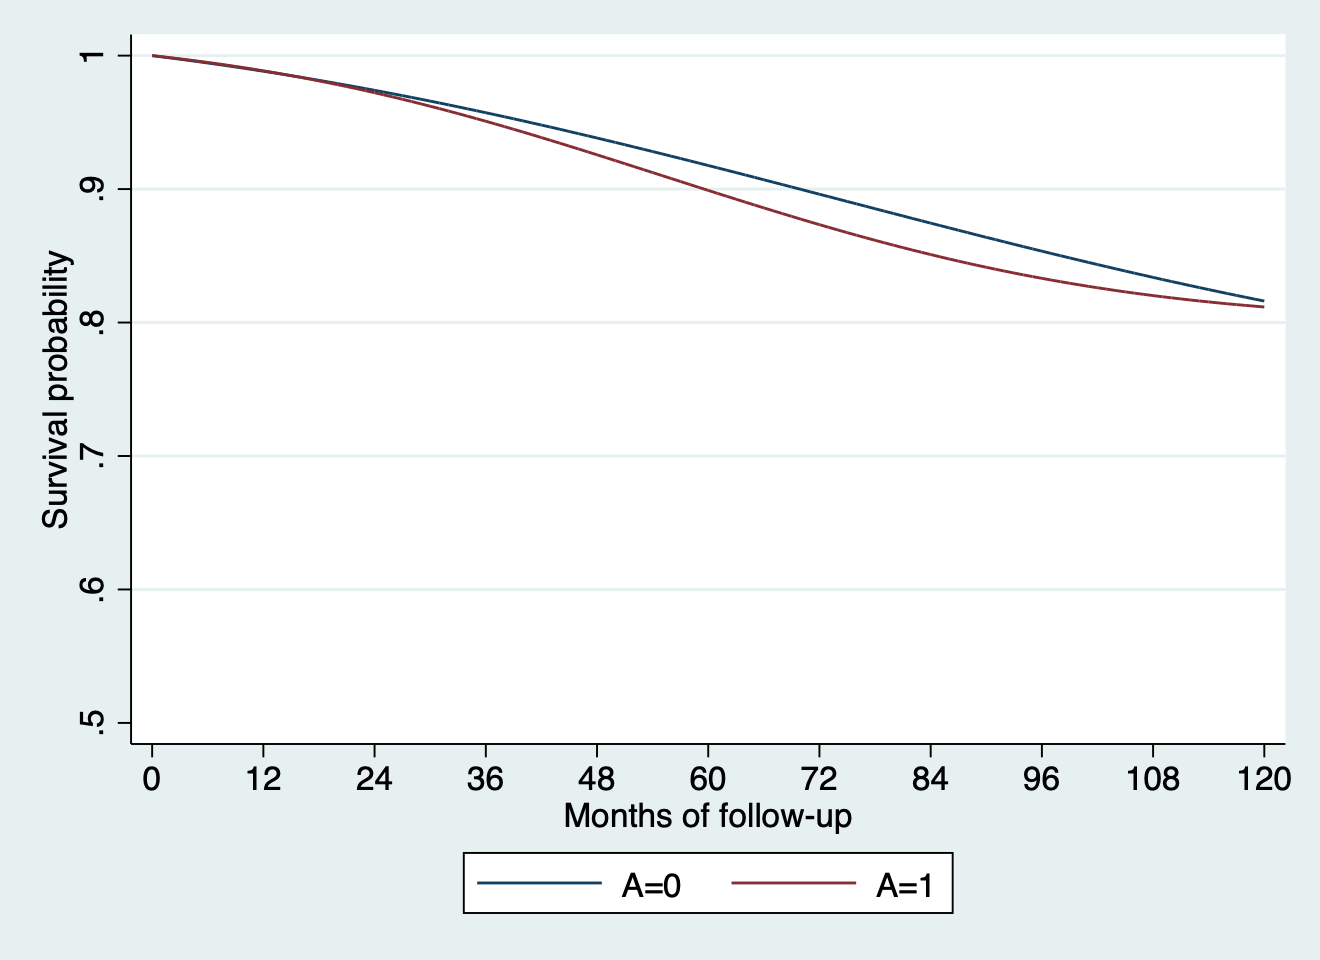
\includegraphics[width=0.85\linewidth]{./figs/stata-fig-17-3} \end{center}

\hypertarget{program-17.4-1}{%
\section{Program 17.4}\label{program-17.4-1}}

\begin{itemize}
\tightlist
\item
  Estimating of survival curves via g-formula
\item
  Data from NHEFS
\item
  Section 17.5
\item
  Generates Figure 17.7
\end{itemize}

\begin{Shaded}
\begin{Highlighting}[]
\KeywordTok{use}\NormalTok{ ./}\KeywordTok{data}\NormalTok{/nhefs\_surv, }\KeywordTok{clear}

\KeywordTok{keep}\NormalTok{ seqn event qsmk time sex race age education }\CommentTok{///}
\NormalTok{  smokeintensity smkintensity82\_71  smokeyrs exercise }\CommentTok{///}
\NormalTok{  active wt71 }
\KeywordTok{preserve}
 
\KeywordTok{quietly} \KeywordTok{logistic}\NormalTok{ event qsmk qsmk\#c.time }\CommentTok{///}
\NormalTok{  qsmk\#c.time\#c.time time c.time\#c.time  }\CommentTok{///}
\NormalTok{    sex race c.age\#\#c.age ib(}\FunctionTok{last}\NormalTok{).education }\CommentTok{///}
\NormalTok{    c.smokeintensity\#\#c.smokeintensity }\CommentTok{///}
\NormalTok{    c.smokeyrs\#\#c.smokeyrs ib(}\FunctionTok{last}\NormalTok{).exercise ib(}\FunctionTok{last}\NormalTok{).active }\CommentTok{///}
\NormalTok{    c.wt71\#\#c.wt71 , }\KeywordTok{cluster}\NormalTok{(seqn) }
            
\KeywordTok{drop} \KeywordTok{if}\NormalTok{ time != 0}
\NormalTok{expand 120 }\KeywordTok{if}\NormalTok{ time ==0 }
\KeywordTok{bysort}\NormalTok{ seqn: }\KeywordTok{replace}\NormalTok{ time = }\DataTypeTok{\_n}\NormalTok{ {-} 1              }
\NormalTok{expand 2 , }\KeywordTok{generate}\NormalTok{(interv) }
\KeywordTok{replace}\NormalTok{ qsmk = interv        }
\KeywordTok{predict}\NormalTok{ pevent\_k, pr}
\KeywordTok{gen}\NormalTok{ psurv\_k = 1{-}pevent\_k}
\KeywordTok{keep}\NormalTok{ seqn  time qsmk interv psurv\_k                 }
\KeywordTok{sort}\NormalTok{ seqn interv time}
\KeywordTok{gen}\NormalTok{ \_t = time + 1}
\KeywordTok{gen}\NormalTok{ psurv = psurv\_k }\KeywordTok{if}\NormalTok{ \_t ==1       }
\KeywordTok{bysort}\NormalTok{ seqn interv: }\KeywordTok{replace}\NormalTok{ psurv = psurv\_k*psurv[\_t{-}1] }\KeywordTok{if}\NormalTok{ \_t \textgreater{}1 }
\KeywordTok{by}\NormalTok{ interv, }\KeywordTok{sort}\NormalTok{: }\KeywordTok{summarize}\NormalTok{ psurv }\KeywordTok{if}\NormalTok{ time == 119}

\KeywordTok{keep}\NormalTok{ qsmk interv psurv time   }
        
\KeywordTok{bysort}\NormalTok{ interv : }\KeywordTok{egen}\NormalTok{ meanS = }\KeywordTok{mean}\NormalTok{(psurv) }\KeywordTok{if}\NormalTok{ time == 119}
\KeywordTok{by}\NormalTok{ interv: }\KeywordTok{summarize}\NormalTok{ meanS}

\KeywordTok{quietly} \KeywordTok{summarize}\NormalTok{ meanS }\KeywordTok{if}\NormalTok{(qsmk==0  \& time ==119)}
\FunctionTok{matrix}\NormalTok{ input observe = ( 0,}\OtherTok{\textasciigrave{}r(mean)\textquotesingle{}}\NormalTok{)}
\KeywordTok{quietly} \KeywordTok{summarize}\NormalTok{ meanS }\KeywordTok{if}\NormalTok{(qsmk==1  \& time ==119)}
\FunctionTok{matrix}\NormalTok{ observe = (observe \textbackslash{}1,}\OtherTok{\textasciigrave{}r(mean)\textquotesingle{}}\NormalTok{)}
\FunctionTok{matrix}\NormalTok{ observe = (observe \textbackslash{}2, observe[2,2]{-}observe[1,2]) }
\NormalTok{*Add some }\OtherTok{row}\NormalTok{/column descriptions and }\KeywordTok{print}\NormalTok{ results to screen*}
\FunctionTok{matrix} \OtherTok{rownames}\NormalTok{ observe =  P(Y(a=0)=1) P(Y(a=1)=1) difference}
\FunctionTok{matrix} \OtherTok{colnames}\NormalTok{ observe = interv survival}

\NormalTok{*Graph standardized survival }\BaseNTok{over}\NormalTok{ time, under interventions*}
\CommentTok{/*Note: unlike in Program 17.3, we now have covariates }
\CommentTok{so we first need to average survival across strata*/}
\KeywordTok{bysort}\NormalTok{ interv time : }\KeywordTok{egen}\NormalTok{ meanS\_t = }\KeywordTok{mean}\NormalTok{(psurv)}

\NormalTok{*Now we can }\KeywordTok{continue}\NormalTok{ with the }\KeywordTok{graph}\NormalTok{*}
\NormalTok{expand 2 }\KeywordTok{if}\NormalTok{ time ==0, }\KeywordTok{generate}\NormalTok{(newtime)}
\KeywordTok{replace}\NormalTok{ meanS\_t  = 1 }\KeywordTok{if}\NormalTok{ newtime == 1}
\KeywordTok{gen}\NormalTok{ time2 = 0 }\KeywordTok{if}\NormalTok{ newtime ==1}
\KeywordTok{replace}\NormalTok{ time2 = time + 1 }\KeywordTok{if}\NormalTok{ newtime == 0}
\KeywordTok{separate}\NormalTok{ meanS\_t, }\KeywordTok{by}\NormalTok{(interv) }

\KeywordTok{twoway}\NormalTok{ (}\KeywordTok{line}\NormalTok{ meanS\_t0 time2, }\KeywordTok{sort}\NormalTok{) }\CommentTok{///}
\NormalTok{  (}\KeywordTok{line}\NormalTok{ meanS\_t1 time2, }\KeywordTok{sort}\NormalTok{) }\CommentTok{///}
\NormalTok{  , }\KeywordTok{ylabel}\NormalTok{(0.5(0.1)1.0) }\KeywordTok{xlabel}\NormalTok{(0(12)120) }\CommentTok{///}
  \BaseNTok{ytitle}\NormalTok{(}\StringTok{"Survival probability"}\NormalTok{) }\BaseNTok{xtitle}\NormalTok{(}\StringTok{"Months of follow{-}up"}\NormalTok{) }\CommentTok{///}
  \BaseNTok{legend}\NormalTok{(}\KeywordTok{label}\NormalTok{(1 }\StringTok{"A=0"}\NormalTok{) }\KeywordTok{label}\NormalTok{(2 }\StringTok{"A=1"}\NormalTok{))}
\KeywordTok{gr} \KeywordTok{export}\NormalTok{ ./figs/stata{-}fig{-}17{-}4.png, }\KeywordTok{replace}

\NormalTok{*remove extra timepoint*}
\KeywordTok{drop} \KeywordTok{if}\NormalTok{ newtime == 1}

\KeywordTok{restore}

\NormalTok{*Bootstraps*}
\KeywordTok{qui} \KeywordTok{save}\NormalTok{ ./}\KeywordTok{data}\NormalTok{/nhefs\_std2 , }\KeywordTok{replace}
 
\KeywordTok{capture} \KeywordTok{program} \KeywordTok{drop}\NormalTok{ bootstdz\_surv}

\KeywordTok{program} \KeywordTok{define}\NormalTok{ bootstdz\_surv , rclass}
\KeywordTok{use}\NormalTok{ ./}\KeywordTok{data}\NormalTok{/nhefs\_std2 , }\KeywordTok{clear}
\KeywordTok{preserve}

\KeywordTok{bsample}\NormalTok{, }\KeywordTok{cluster}\NormalTok{(seqn) idcluster(newseqn)       }
\KeywordTok{logistic}\NormalTok{ event qsmk qsmk\#c.time qsmk\#c.time\#c.time }\CommentTok{///}
\NormalTok{  time c.time\#c.time }\CommentTok{///}
\NormalTok{    sex race c.age\#\#c.age ib(}\FunctionTok{last}\NormalTok{).education }\CommentTok{///}
\NormalTok{    c.smokeintensity\#\#c.smokeintensity c.smkintensity82\_71 }\CommentTok{///}
\NormalTok{    c.smokeyrs\#\#c.smokeyrs ib(}\FunctionTok{last}\NormalTok{).exercise ib(}\FunctionTok{last}\NormalTok{).active }\CommentTok{///}
\NormalTok{    c.wt71\#\#c.wt71 }
\KeywordTok{drop} \KeywordTok{if}\NormalTok{ time != 0   }
\CommentTok{/*only predict on new version of data */}
\NormalTok{expand 120 }\KeywordTok{if}\NormalTok{ time ==0 }
\KeywordTok{bysort}\NormalTok{ newseqn: }\KeywordTok{replace}\NormalTok{ time = }\DataTypeTok{\_n}\NormalTok{ {-} 1               }
\NormalTok{expand 2 , }\KeywordTok{generate}\NormalTok{(interv\_b) }
\KeywordTok{replace}\NormalTok{ qsmk = interv\_b          }
\KeywordTok{predict}\NormalTok{ pevent\_k, pr}
\KeywordTok{gen}\NormalTok{ psurv\_k = 1{-}pevent\_k}
\KeywordTok{keep}\NormalTok{ newseqn  time qsmk psurv\_k                 }
\KeywordTok{sort}\NormalTok{ newseqn qsmk time}
\KeywordTok{gen}\NormalTok{ \_t = time + 1}
\KeywordTok{gen}\NormalTok{ psurv = psurv\_k }\KeywordTok{if}\NormalTok{ \_t ==1   }
\KeywordTok{bysort}\NormalTok{ newseqn  qsmk: }\KeywordTok{replace}\NormalTok{ psurv = psurv\_k*psurv[\_t{-}1] }\KeywordTok{if}\NormalTok{ \_t \textgreater{}1 }
\KeywordTok{drop}  \KeywordTok{if}\NormalTok{ time != 119   }\CommentTok{/* keep only last observation */}
\KeywordTok{keep}\NormalTok{ newseqn qsmk psurv    }
\CommentTok{/* if time is in data for complete graph add time to bysort */}  
\KeywordTok{bysort}\NormalTok{ qsmk  : }\KeywordTok{egen}\NormalTok{ meanS\_b = }\KeywordTok{mean}\NormalTok{(psurv)}
\KeywordTok{keep}\NormalTok{ newseqn qsmk  meanS\_b }
\KeywordTok{drop} \KeywordTok{if}\NormalTok{ newseqn != 1  }\CommentTok{/* only need one pair */}
\KeywordTok{drop}\NormalTok{ newseqn        }
    
\FunctionTok{return} \FunctionTok{scalar}\NormalTok{ boot\_0 = meanS\_b[1]}
\FunctionTok{return} \FunctionTok{scalar}\NormalTok{ boot\_1 = meanS\_b[2]}
\FunctionTok{return} \FunctionTok{scalar}\NormalTok{ boot\_diff = }\FunctionTok{return}\NormalTok{(boot\_1) {-} }\FunctionTok{return}\NormalTok{(boot\_0)}
\KeywordTok{restore}
\KeywordTok{end}

\KeywordTok{set} \DecValTok{rmsg} \KeywordTok{on}
\KeywordTok{simulate}\NormalTok{ PrY\_a0 = }\FunctionTok{r}\NormalTok{(boot\_0) PrY\_a1 = }\FunctionTok{r}\NormalTok{(boot\_1) }\CommentTok{///}
\NormalTok{  difference=}\FunctionTok{r}\NormalTok{(boot\_diff), reps(10) }\DecValTok{seed}\NormalTok{(1): bootstdz\_surv}
\KeywordTok{set} \DecValTok{rmsg} \KeywordTok{off} 
 
\FunctionTok{matrix}\NormalTok{ pe = observe[1..3, 2]\textquotesingle{}}
\KeywordTok{bstat}\NormalTok{, stat(pe) n(1629)}
\end{Highlighting}
\end{Shaded}

\begin{verbatim}
(169,510 observations deleted)

(186,354 observations created)

(186354 real changes made)

(187,920 observations created)

(187,920 real changes made)






(372,708 missing values generated)

(372708 real changes made)


--------------------------------------------------------------------------------
-> interv = Original

    Variable |        Obs        Mean    Std. dev.       Min        Max
-------------+---------------------------------------------------------
       psurv |      1,566    .8160697    .2014345    .014127   .9903372

--------------------------------------------------------------------------------
-> interv = Duplicat

    Variable |        Obs        Mean    Std. dev.       Min        Max
-------------+---------------------------------------------------------
       psurv |      1,566     .811763    .2044758   .0123403   .9900259



(372,708 missing values generated)


--------------------------------------------------------------------------------
-> interv = Original

    Variable |        Obs        Mean    Std. dev.       Min        Max
-------------+---------------------------------------------------------
       meanS |      1,566    .8160697           0   .8160697   .8160697

--------------------------------------------------------------------------------
-> interv = Duplicat

    Variable |        Obs        Mean    Std. dev.       Min        Max
-------------+---------------------------------------------------------
       meanS |      1,566    .8117629           0   .8117629   .8117629










(3,132 observations created)

(3,132 real changes made)

(375,840 missing values generated)

(375,840 real changes made)


Variable      Storage   Display    Value
    name         type    format    label      Variable label
--------------------------------------------------------------------------------
meanS_t0        float   %9.0g                 meanS_t, interv == Original
                                                observation
meanS_t1        float   %9.0g                 meanS_t, interv == Duplicated
                                                observation


file /Users/tom/Documents/GitHub/cibookex-r/figs/stata-fig-17-4.png saved as
    PNG format

(3,132 observations deleted)




  5. drop if time != 0       
  6. /*only predict on new version of data */

r; t=0.00 14:45:59

      Command: bootstdz_surv
       PrY_a0: r(boot_0)
       PrY_a1: r(boot_1)
   difference: r(boot_diff)

Simulations (10)
----+--- 1 ---+--- 2 ---+--- 3 ---+--- 4 ---+--- 5 
..........
r; t=22.61 14:46:22




Bootstrap results                                        Number of obs = 1,629
                                                         Replications  =    10

------------------------------------------------------------------------------
             |   Observed   Bootstrap                         Normal-based
             | coefficient  std. err.      z    P>|z|     [95% conf. interval]
-------------+----------------------------------------------------------------
      PrY_a0 |   .8160697   .0087193    93.59   0.000     .7989802    .8331593
      PrY_a1 |   .8117629   .0292177    27.78   0.000     .7544973    .8690286
  difference |  -.0043068   .0307674    -0.14   0.889    -.0646099    .0559963
------------------------------------------------------------------------------
\end{verbatim}

\begin{center}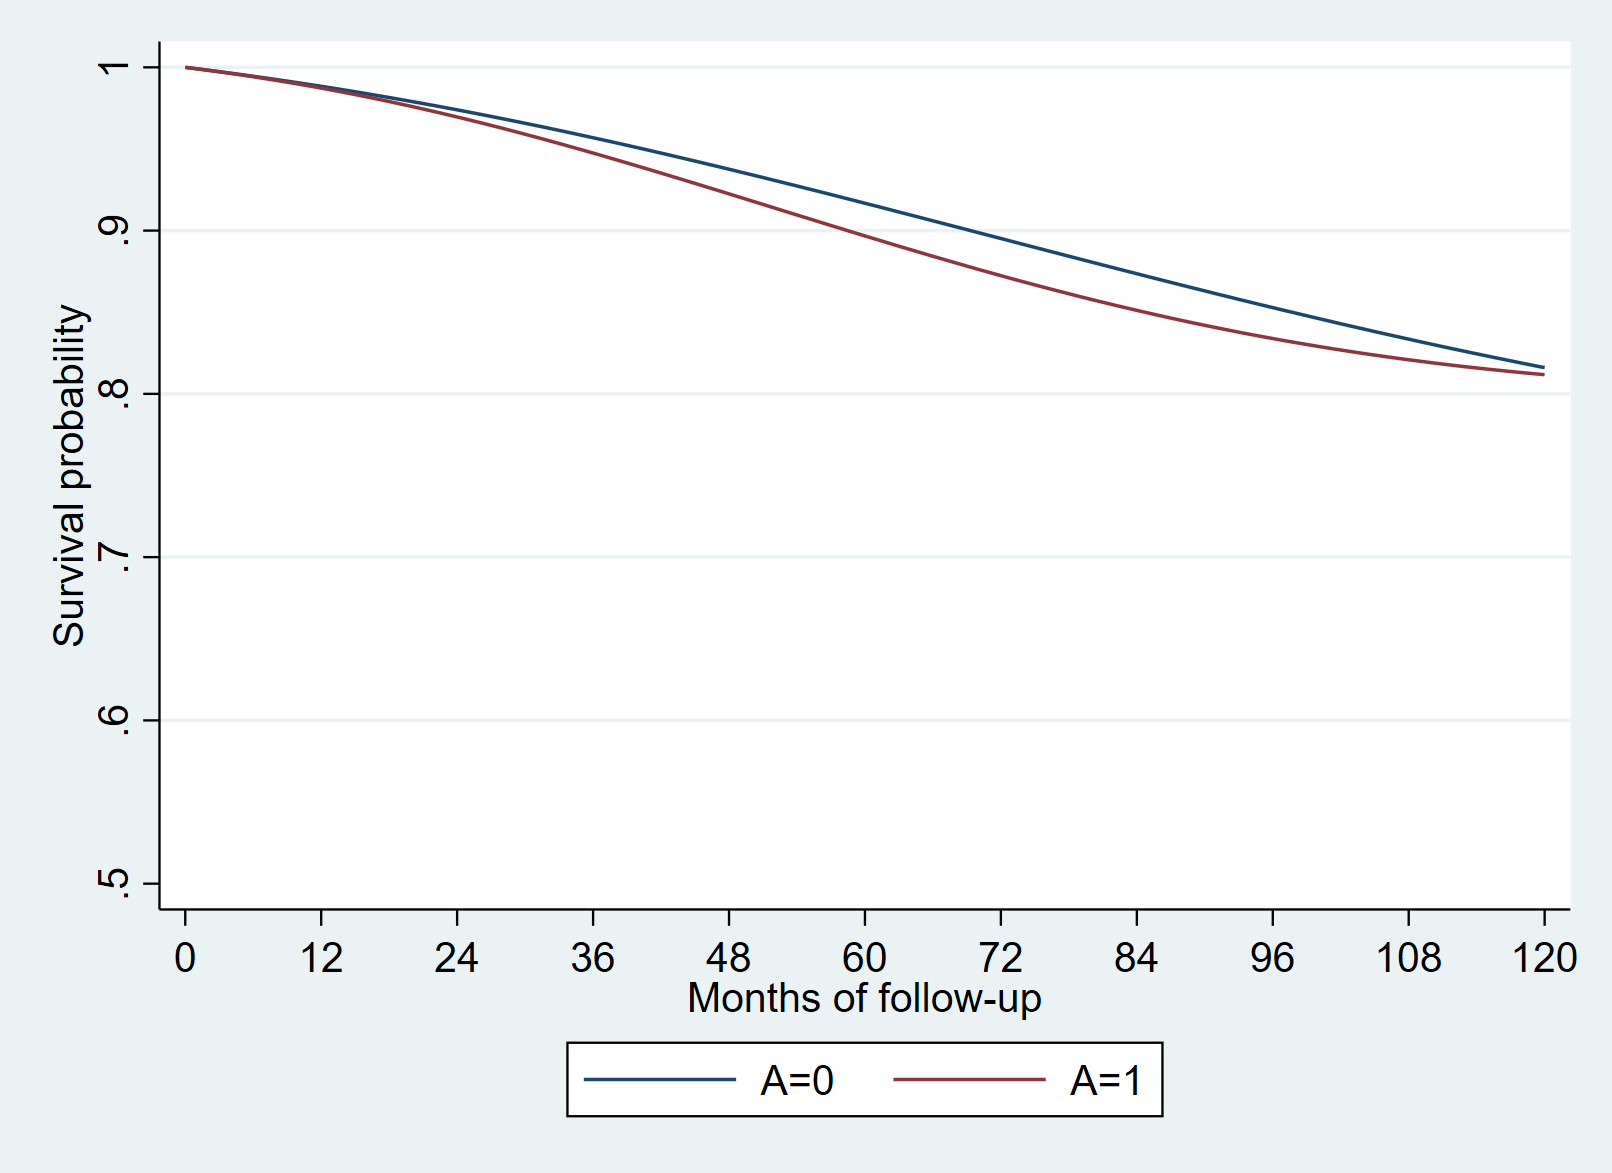
\includegraphics[width=0.85\linewidth]{./figs/stata-fig-17-4} \end{center}

\hypertarget{session-information-stata}{%
\chapter*{Session information: Stata}\label{session-information-stata}}
\addcontentsline{toc}{chapter}{Session information: Stata}

\begin{Shaded}
\begin{Highlighting}[]
\FunctionTok{library}\NormalTok{(Statamarkdown)}
\end{Highlighting}
\end{Shaded}

For reproducibility.

\begin{Shaded}
\begin{Highlighting}[]
\NormalTok{about}
\end{Highlighting}
\end{Shaded}

\begin{verbatim}
Stata/MP 17.0 for Mac (Apple Silicon)
Revision 01 Jun 2022
Copyright 1985-2021 StataCorp LLC

Total physical memory: 8.01 GB

Stata license: Unlimited-user 2-core network, expiring 23 Jan 2023
Serial number: 501709378202
  Licensed to: Tom Palmer
               University of Bristol
\end{verbatim}

\begin{Shaded}
\begin{Highlighting}[]
\CommentTok{\# install.packages("sessioninfo")}
\NormalTok{sessioninfo}\SpecialCharTok{::}\FunctionTok{session\_info}\NormalTok{()}
\end{Highlighting}
\end{Shaded}

\begin{verbatim}
- Session info ---------------------------------------------------------------
 setting  value
 version  R version 4.2.1 (2022-06-23)
 os       macOS Monterey 12.4
 system   aarch64, darwin20
 ui       X11
 language (EN)
 collate  en_GB.UTF-8
 ctype    en_GB.UTF-8
 tz       Europe/London
 date     2022-07-05
 pandoc   2.18 @ /Applications/RStudio.app/Contents/MacOS/quarto/bin/tools/ (via rmarkdown)

- Packages -------------------------------------------------------------------
 package       * version date (UTC) lib source
 bookdown        0.27    2022-06-14 [3] CRAN (R 4.2.0)
 cli             3.3.0   2022-04-25 [3] CRAN (R 4.2.0)
 digest          0.6.29  2021-12-01 [3] CRAN (R 4.2.0)
 evaluate        0.15    2022-02-18 [3] CRAN (R 4.2.0)
 fastmap         1.1.0   2021-01-25 [3] CRAN (R 4.2.0)
 htmltools       0.5.2   2021-08-25 [3] CRAN (R 4.2.0)
 knitr           1.39    2022-04-26 [3] CRAN (R 4.2.0)
 magrittr        2.0.3   2022-03-30 [3] CRAN (R 4.2.0)
 rlang           1.0.3   2022-06-27 [3] CRAN (R 4.2.1)
 rmarkdown       2.14    2022-04-25 [3] CRAN (R 4.2.0)
 rstudioapi      0.13    2020-11-12 [3] CRAN (R 4.2.0)
 sessioninfo     1.2.2   2021-12-06 [3] CRAN (R 4.2.0)
 Statamarkdown * 0.7.1   2022-05-13 [1] Github (Hemken/Statamarkdown@d9cbb1a)
 stringi         1.7.6   2021-11-29 [3] CRAN (R 4.2.0)
 stringr         1.4.0   2019-02-10 [3] CRAN (R 4.2.0)
 xfun            0.31    2022-05-10 [3] CRAN (R 4.2.0)
 yaml            2.3.5   2022-02-21 [3] CRAN (R 4.2.0)

 [1] /Users/tom/Library/R/arm64/4.2/library
 [2] /Library/Frameworks/R.framework/Versions/4.2-arm64/Resources/site-library
 [3] /Library/Frameworks/R.framework/Versions/4.2-arm64/Resources/library

------------------------------------------------------------------------------
\end{verbatim}

  \bibliography{bibliography.bib}

\backmatter

\end{document}
